% db4o 8.1 Manual (Java)
% Build: latexmk -pdf db4o-manual.tex   (or: make)
\documentclass[11pt,openany]{book}

\usepackage[T1]{fontenc}
\usepackage[utf8]{inputenc}
\usepackage{lmodern}
\usepackage{textcomp}
\usepackage[margin=1in]{geometry}
\usepackage{graphicx}
\usepackage{longtable}
\usepackage{array}
\usepackage{xcolor}
\usepackage[normalem]{ulem}
\usepackage{listings}
\usepackage{titlesec}
\usepackage{parskip}
\usepackage{microtype}
\usepackage{xurl}
\setlength{\emergencystretch}{3em}
\usepackage[framemethod=default]{mdframed}
\usepackage[colorlinks=true,linkcolor=blue!50!black,urlcolor=blue!60!black]{hyperref}

% Scale images down to the text width, never up.
\makeatletter
\def\maxwidth{\ifdim\Gin@nat@width>\linewidth\linewidth\else\Gin@nat@width\fi}
\makeatother

\setcounter{secnumdepth}{3}
\setcounter{tocdepth}{2}
\titleformat{\paragraph}{\normalfont\normalsize\bfseries}{\theparagraph}{1em}{}
\titlespacing*{\paragraph}{0pt}{2ex plus 1ex}{0.5ex}
\titleformat{\subparagraph}{\normalfont\normalsize\bfseries\itshape}{\thesubparagraph}{1em}{}
\titlespacing*{\subparagraph}{0pt}{1.5ex plus 1ex}{0.5ex}

\lstset{
  language=Java,
  basicstyle=\ttfamily\small,
  keywordstyle=\color{blue!60!black}\bfseries,
  commentstyle=\color{green!40!black}\itshape,
  stringstyle=\color{red!50!black},
  breaklines=true,
  breakatwhitespace=false,
  columns=fullflexible,
  keepspaces=true,
  showstringspaces=false,
  frame=single,
  rulecolor=\color{black!25},
  backgroundcolor=\color{black!3},
  xleftmargin=2pt, xrightmargin=2pt,
  upquote=true,
}

\newmdenv[linecolor=blue!40,backgroundcolor=blue!4,leftline=true,rightline=false,
  topline=false,bottomline=false,linewidth=2pt]{notebox}

\title{\Huge db4o 8.1\\[1ex]\LARGE Tutorial, Reference and Replication Manual\\[1ex]\large Java Edition}
\author{Converted from the original db4o documentation (Versant Corp.)}
\date{}

\begin{document}
\frontmatter
\maketitle
\tableofcontents
\mainmatter
\part{Tutorial}
% Converted from reference/DB4OTutorial (MadCap Flare, Java target)

\chapter{Introduction}
\label{tut:welcome}

Welcome to the db4o tutorial. In this tutorial we explore the basics of db4o and how to work with it.

\section*{Getting db4o}

db4o is maintained at \href{https://github.com/blakemcbride/db4o}{\nolinkurl{github.com/blakemcbride/db4o}}. Clone or download the repository and build it as described in its \href{https://github.com/blakemcbride/db4o/blob/master/BUILD.md}{\nolinkurl{BUILD.md}} file. The build needs JDK 17 or newer and nothing else:

\begin{lstlisting}
git clone https://github.com/blakemcbride/db4o.git
cd db4o
./bld jar
\end{lstlisting}

This writes the db4o jars to the target directory.

\section*{Adding db4o to a Project}

For this tutorial, add the all-in-one jar to your project:

\begin{itemize}
\item target/db4o-8.1-all.jar
\end{itemize}

A detailed overview of the jars is available in the reference documentation.

\section*{db4o Area of Use}

db4o is intended for embedded use with smaller databases around 2-16 GByte. As a general rule, if you expect your database to grow beyond 16 gigabytes, you should look at a larger database system.

db4o is explicitly single-threaded. Concurrent accesses will be synchronized against a global database lock. That means db4o cannot deal with a highly concurrent access, since it blocks on all operations. When you expect a high load and concurrent access, then you should consider a larger database system.


% Converted from reference/DB4OTutorial (MadCap Flare, Java target)

\chapter{Basics}
\label{tut:basics}

Let's start with the basics. First we create a tiny domain model, consisting out of drivers and cars.

\begin{lstlisting}
public class Car {
    private String carName;

    public Car(String carName) {
        this.carName = carName;
    }

}
\end{lstlisting}

{\small\itshape Car.java: Domain model for cars\par}
\medskip

\begin{lstlisting}
public class Driver {
    private String name;
    private Car mostLovedCar;

    public Driver(String name) {
        this.name = name;
    }

    public Driver(String name, Car mostLovedCar) {
        this.name = name;
        this.mostLovedCar = mostLovedCar;
    }

    public void setName(String name) {
        this.name = name;
    }

    public String getName() {
        return name;
    }

    public Car getMostLovedCar() {
        return mostLovedCar;
    }
}
\end{lstlisting}

{\small\itshape Driver.java: Domain model for drivers\par}
\medskip

\section{Open a Database}
\label{tut:basics:opendb}

For all operations we need to open the database first. To open the database we pass a file-path to db4o. db4o will open or create that database-file an return an object container. The object container is the connection to our database. All operations go through it.

\begin{lstlisting}
ObjectContainer container = Db4oEmbedded.openFile("database.db4o");
try{
    // use the object container in here
} finally {
    container.close();
}
\end{lstlisting}

{\small\itshape BasicOperations.java: Open and close db4o\par}
\medskip

\section{Store an Object}
\label{tut:basics:storeobject}

To store an object in the database, we simply call the store-method on the object container.

\begin{lstlisting}
ObjectContainer container = Db4oEmbedded.openFile("databaseFile.db4o");
try {
    Driver driver = new Driver("Joe");
    container.store(driver);
} finally {
    container.close();
}
\end{lstlisting}

{\small\itshape BasicOperations.java: Store an object\par}
\medskip

\section{Query the Database}
\label{tut:basics:querydb}

After storing objects we want to query for our stored objects. We can do this with native queries.

\begin{lstlisting}
ObjectContainer container = Db4oEmbedded.openFile("databaseFile.db4o");
try {
    List<Driver> drivers = container.query(new Predicate<Driver>() {
        public boolean match(Driver d) {
            return d.getName().equals("Joe");
        }
    });
    System.out.println("Stored Pilots:");
    for (Driver driver : drivers) {
        System.out.println(driver.getName());
    }
} finally {
    container.close();
}
\end{lstlisting}

{\small\itshape BasicOperations.java: Query for objects\par}
\medskip

\section{Update an Object}
\label{tut:basics:updateobject}

In order to update an object we first query for it. Then we change it and store it again. db4o will recognize the updated object and store the changes in the database.

\begin{lstlisting}
ObjectContainer container = Db4oEmbedded.openFile("databaseFile.db4o");
try {
    List<Driver> drivers = container.query(new Predicate<Driver>() {
        public boolean match(Driver d) {
            return d.getName().equals("Joe");
        }
    });
    Driver driver = drivers.get(0);
    System.out.println("Old name" +driver.getName());
    driver.setName("John");
    System.out.println("New name" +driver.getName());
    // update the pilot
    container.store(driver);
} finally {
    container.close();
}
\end{lstlisting}

{\small\itshape BasicOperations.java: Update an object\par}
\medskip

\section{Delete an Object}
\label{tut:basics:deleteobject}

Deleting an object is easy. First we query for the object and then delete it.

\begin{lstlisting}
ObjectContainer container = Db4oEmbedded.openFile("databaseFile.db4o");
try {
    List<Driver> drivers = container.query(new Predicate<Driver>() {
        public boolean match(Driver d) {
            return d.getName().equals("Joe");
        }
    });
    Driver driver = drivers.get(0);
    System.out.println("Deleting " +driver.getName());
    container.delete(driver);
} finally {
    container.close();
}
\end{lstlisting}

{\small\itshape BasicOperations.java: Delete an object\par}
\medskip


% Converted from reference/DB4OTutorial (MadCap Flare, Java target)

\chapter{Queries}
\label{tut:queries}

Let's take a look at a few examples queries.

\begin{lstlisting}
public class Car {
    private String carName;
    private int horsePower;

    public Car(String carName, int horsePower) {
        this.carName = carName;
        this.horsePower = horsePower;
    }

    public String getCarName() {
        return carName;
    }

    public int getHorsePower() {
        return horsePower;
    }

    @Override
    public String toString() {
        return "Car{" +
                "carName='" + carName + '\'' +
                ", horsePower=" + horsePower +
                '}';
    }
}
\end{lstlisting}

{\small\itshape Car.java: Domain model for cars\par}
\medskip

\begin{lstlisting}
public class Driver {
    private String name;
    private int age;
    private Car mostLovedCar;

    public Driver(String name,int age) {
        this.name = name;
        this.age = age;
    }

    public Driver(String name,int age, Car mostLovedCar) {
        this.name = name;
        this.age = age;
        this.mostLovedCar = mostLovedCar;
    }

    public void setName(String name) {
        this.name = name;
    }

    public String getName() {
        return name;
    }

    public int getAge() {
        return age;
    }

    public Car getMostLovedCar() {
        return mostLovedCar;
    }

    @Override
    public String toString() {
        return "Driver{" +
                "name='" + name + '\'' +
                ", age=" + age +
                ", mostLovedCar=" + mostLovedCar +
                '}';
    }
}
\end{lstlisting}

{\small\itshape Driver.java: Domain model for drivers\par}
\medskip

\section{Native Queries}
\label{tut:queries:nativequeries}

Native queries are the preferred way to query a db4o database. To query the database, we pass in a predicate which filters objects by their properties. Here are two example queries:

\subsection*{Query for a Certain Person}

This query finds all drivers named Joe:

\begin{lstlisting}
List<Driver> drivers = container.query(new Predicate<Driver>() {
    @Override
    public boolean match(Driver driver) {
        return driver.getName().equals("Joe");
    }
});
\end{lstlisting}

{\small\itshape Queries.java: Query for drivers named Joe\par}
\medskip

\subsection*{More Complex Query}

We can combine many criteria in a query by using logical operators. For example we query for all adult drivers with powerful cars by combining multiple criteria.

\begin{lstlisting}
List<Driver> drivers = container.query(new Predicate<Driver>() {
    @Override
    public boolean match(Driver driver) {
        return driver.getMostLovedCar().getHorsePower()>=150 && driver.getAge()>=18;
    }
});
\end{lstlisting}

{\small\itshape Queries.java: Query for people with powerful cars\par}
\medskip

\subsection*{Native Query Optimization}

db4o tries to optimize native queries by translating them to the db4o low level query API. In cases which that doesn't work db4o actually instantiates all objects and runs them through the predicate. Unfortunately that's an order of magnitude slower than an optimized query.

How do we find out that a query couldn't be optimized? The simplest way is to use the debugger. We add a break-point in query method. When the debugger stops there, then query couldn't be optimized. In that case try to simplify our query or use the low level query API directly.

\begin{lstlisting}
List<Driver> drivers = container.query(new Predicate<Driver>() {
    @Override
    public boolean match(Driver driver) {
        // Add a break point here. If the debugger stops, the query couldn't be optimized
        // That means it runs very slowly and we should find an alternative.
        // This example query cannot be optimized because the hash code isn't a stored in database
        return driver.hashCode() == 42;
    }
});
\end{lstlisting}

{\small\itshape Queries.java: Unoptimized query\par}
\medskip

\section{SODA}
\label{tut:queries:soda}

SODA is db4o's low level query API. Prefer native queries over this API. We create SODA queries by creating a query object. Then we add different criteria to that query object. Finally we execute the query and get the result. Let's take a look at two example queries:

\subsection*{Query for a Certain Person}

Here we query for a driver named Joe with SODA:

\begin{lstlisting}
Query query = container.query();
query.constrain(Driver.class);
query.descend("name").constrain("Joe");
List<Driver> drivers = query.execute();
\end{lstlisting}

{\small\itshape Queries.java: Query for drivers named Joe with SODA\par}
\medskip

\subsection*{More Complex Query}

Here's a more complex query in SODA. We query for all adult drivers with powerful cars:

\begin{lstlisting}
Query query = container.query();
query.constrain(Driver.class);
query.descend("mostLovedCar").descend("horsePower").constrain(150).greater();
query.descend("age").constrain(18).greater().equal();
List<Driver> drivers = query.execute();
\end{lstlisting}

{\small\itshape Queries.java: Query for people with powerful cars with SODA\par}
\medskip


% Converted from reference/DB4OTutorial (MadCap Flare, Java target)

\chapter{Activation}
\label{tut:activation}

Activation is a mechanism which controls object instantiation. Why is this necessary? Let's look at an example. We store person-objects with its parents. Each person object has a reference to his parents, the parents again have references to their parents and so on and so forth. Now we load a person object from the database, what does db4o do? Does it load the person object, its parents and the parents of the parents? Then it probably loads all objects from the database and will use up all memory.

\begin{center}
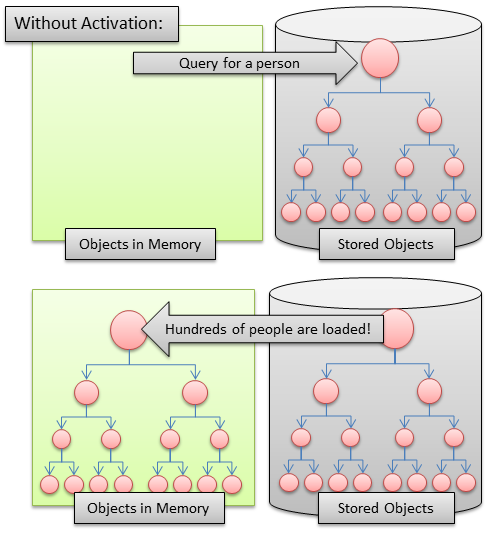
\includegraphics[width=\maxwidth]{images/tut-without-activation.png}
\end{center}
Luckily db4o does not behave like this. When a query retrieves objects, their fields are loaded into memory (activated in db4o terms) only to a certain activation depth. In this case depth means "number of member references away from the original object". All the fields beyond the activation depth are set to null or to default values.So db4o does not load the whole object graph at once. Instead, db4o loads only the parts which we are interested in.

\begin{center}
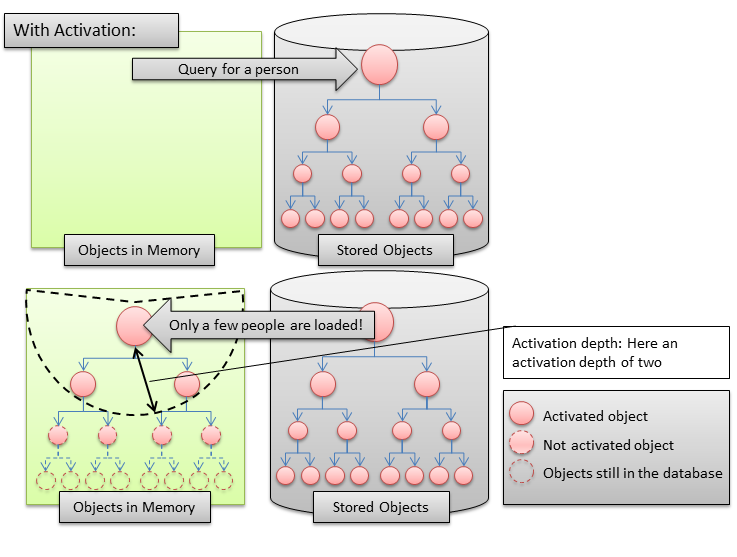
\includegraphics[width=\maxwidth]{images/tut-with-activation.png}
\end{center}
\section{Activation in Action}
\label{tut:activation:activationinaction}

Let's see db4o's activation in action. To do so we need a deep object-graph. We create a person class with a mother-field and then create a deep hierarchy of people, for example a hierarchy of seven people.

\begin{lstlisting}
public class Person {
    private String name;
    private Person mother;

    public Person(String name, Person mother) {
        this.name = name;
        this.mother = mother;
    }

    public String getName() {
        return name;
    }

    public Person getMother() {
        return mother;
    }

    @Override
    public String toString() {
        return "Person{" +
                "name='" + name +
                "'}";
    }
}
\end{lstlisting}

{\small\itshape Person.java: Domain model for people\par}
\medskip

\begin{lstlisting}
Person eva = new Person("Eva",null);
Person julia = new Person("Julia",eva);
Person jennifer = new Person("Jennifer",julia);
Person jamie = new Person("Jamie",jennifer);
Person jill = new Person("Jill",jamie);
Person joanna = new Person("Joanna",jill);

Person joelle = new Person("Joelle",joanna);
container.store(joelle);
\end{lstlisting}

{\small\itshape ActivationConcept.java: Store a deep object hierarchy\par}
\medskip

After that we close the database, reopen it and query for a person. Then we start to traverse the object graph. At a certain point we will reach objects which aren't activated anymore. In those objects all fields are null or have the default value:

\begin{lstlisting}
Person joelle = queryForJoelle(container);
Person jennifer = joelle.getMother().getMother().getMother().getMother();
System.out.println("Is activated: " + jennifer);
// Now we step across the activation boundary
// therefore the next person isn't activate anymore.
// That means all fields are set to null or default-value
Person julia = jennifer.getMother();
System.out.println("Isn't activated anymore"+julia);
\end{lstlisting}

{\small\itshape ActivationConcept.java: Activation depth in action\par}
\medskip

Since not activate objects have set all their fields to null, they can cause null pointer exceptions:

\begin{lstlisting}
String nameOfMother = julia.getMother().getName();
\end{lstlisting}

{\small\itshape ActivationConcept.java: NullPointer exception due to not activated objects\par}
\medskip

\section{Deal With Activation}
\label{tut:activation:dealwithactivation}

We've seen that activation can cause issues and we have to deal with it. There are different strategies for that.

\subsection*{Directly Activating Objects}

We can explicitly activate objects or ask about their activation state. This way we can activate objects when needed. However as soon as we need to activate objects explicitly all over the place in our code we should look for alternatives.

\begin{lstlisting}
boolean isActivated = container.ext().isActive(julia);
\end{lstlisting}

{\small\itshape ActivationConcept.java: Check if an instance is activated\par}
\medskip

\begin{lstlisting}
container.activate(julia,5);
\end{lstlisting}

{\small\itshape ActivationConcept.java: Activate instance to a depth of five\par}
\medskip

\subsection*{Changing Activation Depth}

Alternatively we can increase the activation depth globally or for certain types. However we need to be aware that a high activation depth decreases performance. That's why we should be very careful with increasing the activation depth.

\begin{lstlisting}
EmbeddedConfiguration configuration = Db4oEmbedded.newConfiguration();
configuration.common().activationDepth(10);
ObjectContainer container = Db4oEmbedded.openFile(configuration,DATABASE_FILE);
\end{lstlisting}

{\small\itshape ActivationConcept.java: Increase the activation depth to 10\par}
\medskip

We can even more fine tune the activation depth. However the fundamental issue is the same. When we increase the activation depth it will hurt performance.

\begin{lstlisting}
EmbeddedConfiguration configuration = Db4oEmbedded.newConfiguration();
// At least activate persons to a depth of 10
configuration.common().objectClass(Person.class).minimumActivationDepth(10);
// Or maybe we just want to activate all referenced objects
configuration.common().objectClass(Person.class).cascadeOnActivate(true);
\end{lstlisting}

{\small\itshape ActivationConcept.java: More activation options\par}
\medskip

\subsection*{Transparent Activation / Persistence}

The last option we have is transparent activation. Transparent activation takes care of all activation issues. It activates objects as soon as they are needed. To get transparent activation we need to enhance our classes at compile time. Read \hyperref[tut:transparentpersistence]{this section of the tutorial} (p.~\pageref{tut:transparentpersistence}) where we use transparent activation.


% Converted from reference/DB4OTutorial (MadCap Flare, Java target)

\chapter{Update Concept}
\label{tut:update-concept}

How does updating objects work with db4o? Similar to the activation depth, db4o uses an update depth. When we store an object again, db4o only updates the objects up to the given update-depth. This prevents db4o from traversing the whole object graph in order to store the changes.

\begin{center}
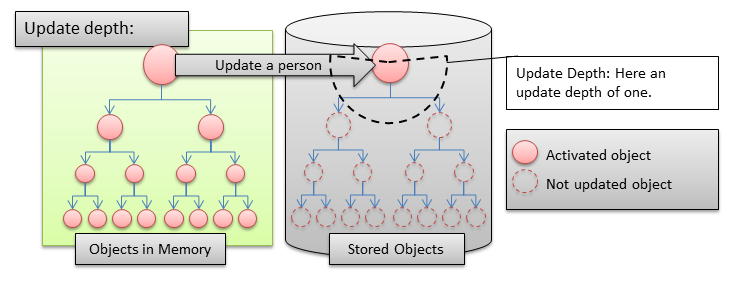
\includegraphics[width=\maxwidth]{images/tut-update-depth.png}
\end{center}
\section{Updating in Action}
\label{tut:update-concept:updatedepthinaction}

Let's see db4o's update strategy in action. We store a driver with his cars and his most loved car.

\begin{lstlisting}
public class Car {
    private String carName;

    public Car(String carName) {
        this.carName = carName;
    }

    public String getCarName() {
        return carName;
    }

    public void setCarName(String carName) {
        this.carName = carName;
    }

    @Override
    public String toString() {
        return "Car{" +
                "carName='" + carName + '\'' +
                '}';
    }
}
\end{lstlisting}

{\small\itshape Car.java: Domain model for cars\par}
\medskip

\begin{lstlisting}
public class Driver {
    private String name;
    private final List<Car> ownedCars = new ArrayList<Car>();
    private Car mostLovedCar;

    public Driver(String name) {
        this.name = name;
    }

    public Driver(String name, Car mostLovedCar) {
        this.name = name;
        this.mostLovedCar = mostLovedCar;
    }

    public void setName(String name) {
        this.name = name;
    }

    public String getName() {
        return name;
    }

    public Car getMostLovedCar() {
        return mostLovedCar;
    }

    public Iterable<Car> getOwnedCars() {
        return ownedCars;
    }

    public boolean addOwnedCar(Car car) {
        return ownedCars.add(car);
    }
}
\end{lstlisting}

{\small\itshape Driver.java: Domain model for drivers\par}
\medskip

\begin{lstlisting}
Car beetle = new Car("VW Beetle");
Car ferrari = new Car("Ferrari");

Driver driver = new Driver("John", ferrari);
driver.addOwnedCar(beetle);
driver.addOwnedCar(ferrari);

container.store(driver);
\end{lstlisting}

{\small\itshape UpdateConcept.java: Store a driver and his cars\par}
\medskip

After that we update the driver, change the name of his most loved car and add another car to his collection. Then we update the car in the database.

\begin{lstlisting}
Driver driver = queryForDriver(container);
driver.setName("Johannes");
driver.getMostLovedCar().setCarName("Red Ferrari");
driver.addOwnedCar(new Car("Fiat Punto"));
container.store(driver);
\end{lstlisting}

{\small\itshape UpdateConcept.java: Update the driver and his cars\par}
\medskip

Then we close the database, reopen it and check if the objects have been updated. Unfortunately only the car itself has been updated. That's because db4o by default uses an update-depth of one. That means only the object we pass to the store-method is updated. All referenced objects are not updated. In our case that means that the referenced car and the referenced list of cars isn't updated.

\begin{lstlisting}
Driver driver = queryForDriver(container);
// Is updated
System.out.println(driver.getName());
// Isn't updated at all
System.out.println(driver.getMostLovedCar().getCarName());
// Also the owned car list isn't updated
for (Car car : driver.getOwnedCars()) {
    System.out.println(car);
}
\end{lstlisting}

{\small\itshape UpdateConcept.java: Check the updated objects\par}
\medskip

\section{Deal with Updates}
\label{tut:update-concept:dealwithit}

We've seen that by default only the object passed to the store method is updated. That means we need a strategy to deal with this.

\subsection*{Explicitly Storing Every Changed Object}

One way to deal with this is to store every changed object. In our case that would be the driver, the most loved car and the list of owed cars. However in practice this strategy needs too much effort.

\begin{lstlisting}
container.store(driver);
container.store(driver.getMostLovedCar());
container.store(driver.getOwnedCars());
\end{lstlisting}

{\small\itshape UpdateConcept.java: Update everything explicitly\par}
\medskip

\subsection*{Change the Activation Depth}

A simple strategy is to increase the update depth, for example increase the depth to two. This is quite a reasonable update-depth, especially since it will update collections of an object.

\begin{lstlisting}
EmbeddedConfiguration configuration = Db4oEmbedded.newConfiguration();
configuration.common().updateDepth(2);
\end{lstlisting}

{\small\itshape UpdateConcept.java: Increase the update depth to 2\par}
\medskip

We can control the update-depth also per class:

\begin{lstlisting}
EmbeddedConfiguration configuration = Db4oEmbedded.newConfiguration();
// Update all referenced objects for the Driver class
configuration.common().objectClass(Driver.class).cascadeOnUpdate(true);
\end{lstlisting}

{\small\itshape UpdateConcept.java: More update options\par}
\medskip

\subsection*{Transparent Persistence}

The last and most elaborate option is to use transparent persistence. In that case db4o manages all updates for us. We just can change objects and db4o will track all changes for us. To get transparent persistence we need to enhance our classes at compile time. Read \hyperref[tut:transparentpersistence]{this section of the tutorial} (p.~\pageref{tut:transparentpersistence}) where we use transparent persistence.


% Converted from reference/DB4OTutorial (MadCap Flare, Java target)

\chapter{Transparent Persistence}
\label{tut:transparentpersistence}

In the previous topics we've seen that \hyperref[tut:activation]{activation} (p.~\pageref{tut:activation}) and the \hyperref[tut:update-concept]{update depth} (p.~\pageref{tut:update-concept}) can be annoying and cause unexpected errors. That's why we want to get rid of it. That's where transparent persistence comes to our rescue. It manages the activation and updating of our updates. Let's get started.

\section{Enhance Persistent Classes}
\label{tut:transparentpersistence:enhance}

The first step for transparent persistence it to enhance the persisted classes. For that we introduce an Annotation:

\begin{lstlisting}
@Retention(RetentionPolicy.RUNTIME)
@Documented
@Target(ElementType.TYPE)
public @interface TransparentPersisted {
}
\end{lstlisting}

{\small\itshape TransparentPersisted.java: Annotation to mark persisted classes\par}
\medskip

After that we can mark the persistent classes with the Annotation.

\begin{lstlisting}
@TransparentPersisted
public class Car {
    private String carName;

    public Car(String carName) {
        this.carName = carName;
    }

    public String getCarName() {
        return carName;
    }

    public void setCarName(String carName) {
        this.carName = carName;
    }
}
\end{lstlisting}

{\small\itshape Car.java: Domain model for cars\par}
\medskip

\begin{lstlisting}
@TransparentPersisted
public class Driver {
    private String name;
    private final List<Car> ownedCars = new ArrayList<Car>();
    private Car mostLovedCar;

    public Driver(String name) {
        this.name = name;
    }

    public Driver(String name, Car mostLovedCar) {
        this.name = name;
        this.mostLovedCar = mostLovedCar;
    }

    public void setName(String name) {
        this.name = name;
    }

    public String getName() {
        return name;
    }

    public Car getMostLovedCar() {
        return mostLovedCar;
    }
    public Iterable<Car> getOwnedCars() {
        return ownedCars;
    }

    public boolean addOwnedCar(Car car) {
        return ownedCars.add(car);
    }
}
\end{lstlisting}

{\small\itshape Driver.java: Domain model for drivers\par}
\medskip

The next step it to create a class filter which reports all classes which should be enhanced. In our example we check for the presence of the annotation. In practice you can implement your own class filter as you like.

\begin{lstlisting}
public final class AnnotationFilter implements ClassFilter{

    public boolean accept(Class<?> aClass) {
        if(null==aClass || aClass.equals(Object.class)){
            return false;
        }
        return hasAnnotation(aClass)
                || accept(aClass.getSuperclass());
    }

    private boolean hasAnnotation(Class<?> aClass) {
        // We compare by name, to be class-loader independent
        Annotation[] annotations = aClass.getAnnotations();
        for (Annotation annotation : annotations) {
            if(annotation.annotationType().getName()
                    .equals(TransparentPersisted.class.getName())){
                return true;
            }
        }
        return false;
    }

}
\end{lstlisting}

{\small\itshape AnnotationFilter.java: Build a filter\par}
\medskip

\subsection*{Enhancing Classes Using Ant}

The next step is to run the enhancement step when compiling the source. You can do this with a Ant task.

\begin{lstlisting}
<target name="enhance">
    <!-- Change these according to your project -->
    <property name="target" value="./target/classes/"/>
    <property name="libraries" value="./lib/"/>

    <path id="project.classpath">
        <pathelement path="${target}"/>
        <fileset dir="${libraries}">
            <include name="*.jar"/>
        </fileset>
    </path>

    <!-- We enhance with an additional Ant-run step. You can put this also in an extra file -->
    <typedef resource="instrumentation-def.properties"
             classpathref="project.classpath"
             loaderRef="instrumentation.loader"/>

    <!-- We filter by our annotation -->
    <typedef name="annotation-filter"
             classname="com.db4odoc.tutorial.transparentpersistence.AnnotationFilter"
             classpathref="project.classpath"
             loaderRef="instrumentation.loader"/>

    <db4o-instrument classTargetDir="${target}">
        <classpath refid="project.classpath"/>
        <sources dir="${target}">
            <include name="**/*.class"/>
        </sources>

        <transparent-activation-step>
            <annotation-filter/>
        </transparent-activation-step>
    </db4o-instrument>
</target>
\end{lstlisting}

{\small\itshape enhance.xml: Ant target for enhancing your classes after building them\par}
\medskip

We can configure Eclipse to run the Ant build with each compile step. Right click on our project and choose 'Properties'. Then switch to 'Builders' and add a new one. The we choose the 'Ant Builder'. On the new window we choose the build-file which contains the example-code.Then switch to the 'Targets'-Tab. There we choose the enhance-target for the 'Auto-Build'. Now the enhancer-task will be run by Eclipse automatically.

\subsection*{Enhance Classes Using Maven}

The next step is to run the enhancement step when compiling the source. You can do this by adding a small Ant task to your Maven file:

\begin{lstlisting}
<plugin>
    <artifactId>maven-antrun-plugin</artifactId>
    <version>1.6</version>
    <dependencies>
        <!-- We need the db4o tooling for enhancing stuff -->
        <dependency>
            <groupId>com.db4o</groupId>
            <artifactId>db4o-tools-java5</artifactId>
            <version>8.1-SNAPSHOT</version>
        </dependency>
    </dependencies>
    <executions>
        <execution>
            <phase>compile</phase>
            <configuration>
                <target>
                    <!-- We enhance with an additional Ant-run step. You can put this also in an extra file -->
                    <typedef resource="instrumentation-def.properties"
                             classpathref="maven.compile.classpath"/>

                    <!-- We filter by our annotation -->
                    <typedef name="annotation-filter"
                             classname="com.db4odoc.tutorial.transparentpersistence.AnnotationFilter"
                             classpathref="maven.compile.classpath"/>

                    <db4o-instrument classTargetDir="target/classes">
                        <classpath refid="maven.compile.classpath"/>
                        <sources dir="target/classes">
                            <include name="**/*.class"/>
                        </sources>

                        <transparent-activation-step>
                            <annotation-filter/>
                        </transparent-activation-step>
                    </db4o-instrument>
                </target>
            </configuration>
            <goals>
                <goal>run</goal>
            </goals>
        </execution>
    </executions>
</plugin>
\end{lstlisting}

{\small\itshape pom.xml: Enhance persisted classes during the build\par}
\medskip

\subsection*{Check Enhancement}

Finally we check if the enhancement actually worked. We just check if the classes implement the interface. If the interface is present everything worked. We can make this check a part of our test suite.

\begin{lstlisting}
if (!Activatable.class.isAssignableFrom(Car.class)) {
    throw new AssertionError("Expect that the " + Car.class + " implements " + Activatable.class);
}
\end{lstlisting}

{\small\itshape TransparentPersistence.java: Check for enhancement\par}
\medskip

\section{Using Transparent Persistence}
\label{tut:transparentpersistence:usingit}

In order to use transparent persistence we need to configure it first:

\begin{lstlisting}
final EmbeddedConfiguration configuration = Db4oEmbedded.newConfiguration();
configuration.common().add(new TransparentPersistenceSupport(new DeactivatingRollbackStrategy()));
ObjectContainer container = Db4oEmbedded.openFile(configuration, DATABASE_FILE_NAME);
\end{lstlisting}

{\small\itshape TransparentPersistence.java: Configure transparent persistence\par}
\medskip

After that transparent persistence is active and manages the activation and updates for us.

\begin{lstlisting}
Driver driver = queryForDriver(container);
// Transparent persistence will activate objects as needed
System.out.println("Is activated? "+container.ext().isActive(driver));
String nameOfDriver = driver.getName();
System.out.println("The name is "+nameOfDriver);
System.out.println("Is activated? "+container.ext().isActive(driver));
\end{lstlisting}

{\small\itshape TransparentPersistence.java: Transparent persistence manages activation\par}
\medskip

Transparent persistence also manages updates. You just can change existing objects as you please. Later when you commit the transaction all updates are persisted. You don't need to store objects in order to update them. You only need to call store once for objects which are new and are not referenced by an existing object.

\begin{lstlisting}
Driver driver = queryForDriver(container);
driver.getMostLovedCar().setCarName("New name");
driver.setName("John Turbo");
driver.addOwnedCar(new Car("Volvo Combi"));
// Just commit the transaction. All modified objects are stored
container.commit();
\end{lstlisting}

{\small\itshape TransparentPersistence.java: Just update and commit. Transparent persistence manages all updates\par}
\medskip


% Converted from reference/DB4OTutorial (MadCap Flare, Java target)

\chapter{Transactions}
\label{tut:transactions}

db4o has ACID properties and supports transactions. Now we take a look at db4o's transaction support.

\begin{lstlisting}
@TransparentPersisted
public class Car {
    private String carName;

    public Car(String carName) {
        this.carName = carName;
    }

    public String getCarName() {
        return carName;
    }
}
\end{lstlisting}

{\small\itshape Car.java: Domain model for cars\par}
\medskip

\begin{lstlisting}
@TransparentPersisted
public class Driver {
    private String name;
    private Car mostLovedCar;

    public Driver(String name) {
        this.name = name;
    }

    public Driver(String name, Car mostLovedCar) {
        this.name = name;
        this.mostLovedCar = mostLovedCar;
    }

    public void setName(String name) {
        this.name = name;
    }

    public String getName() {
        return name;
    }

    public Car getMostLovedCar() {
        return mostLovedCar;
    }
}
\end{lstlisting}

{\small\itshape Driver.java: Domain model for drivers\par}
\medskip

\section{Commit and Rollback}
\label{tut:transactions:commitrollback}

db4o starts a transaction as soon as you open an object container and implicitly commits it when you close the object container. In between we can control the transaction explicitly by calling the commit or rollback method. After the commit everything is persisted and another transaction is started.

\begin{lstlisting}
container.commit();
\end{lstlisting}

{\small\itshape Transactions.java: Committing changes\par}
\medskip

The same applies to rollbacks. We can rollback the transaction any time. After a rollback the next transaction is started.

\begin{lstlisting}
container.rollback();
\end{lstlisting}

{\small\itshape Transactions.java: Rollback changes\par}
\medskip

\section{Object State After Rollback}
\label{tut:transactions:objectstate}

What happens to objects in memory when we rollback a transaction? By default the objects in memory keep their state. If you want to rollback the objects in memory you need to reload them.

\begin{lstlisting}
Driver driver = queryForDriver(container);
driver.setName("New Name");
System.out.println("Name before rollback " + driver.getName());
container.rollback();
// Without transparent persistence objects keep the state in memory
System.out.println("Name after rollback " + driver.getName());
// After refreshing the object is has the state like in the database
container.ext().refresh(driver, Integer.MAX_VALUE);
System.out.println("Name after rollback " + driver.getName());
\end{lstlisting}

{\small\itshape Transactions.java: Without transparent persistence objects in memory aren't rolled back\par}
\medskip

\subsection*{With Transparent Persistence}

With transparent activation we can use a rollback strategy. That way we can rollback the state of the objects in memory.

\begin{lstlisting}
EmbeddedConfiguration configuration = Db4oEmbedded.newConfiguration();
configuration.common().add(new TransparentPersistenceSupport(new DeactivatingRollbackStrategy()));
\end{lstlisting}

{\small\itshape Transactions.java: Rollback strategy for the transaction\par}
\medskip

\begin{lstlisting}
Driver driver = queryForDriver(container);
driver.setName("New Name");
System.out.println("Name before rollback " + driver.getName());
container.rollback();
// Thanks to transparent persistence with the rollback strategy
// the object state is rolled back
System.out.println("Name after rollback " + driver.getName());
\end{lstlisting}

{\small\itshape Transactions.java: Transparent persistence rolls back objects in memory\par}
\medskip

\section{Multiple Transactions}
\label{tut:transactions:multipletx}

For more complex applications we can use multiple transactions. For that we need to create multiple object containers, each having its own transaction.

When we have multiple object containers, an object always needs to be loaded and stored in the same object container.

\begin{lstlisting}
ObjectContainer container = rootContainer.ext().openSession();
try{
    // We do our operations in this transaction
} finally {
    container.close();
}
\end{lstlisting}

{\small\itshape Transactions.java: Opening a new transaction\par}
\medskip


% Converted from reference/DB4OTutorial (MadCap Flare, Java target)

\chapter{Indexes}
\label{tut:indexes}

With indexes we can speed up queries. As soon as we have lots of objects and query them we need indexes.

Indexes are a tradeoff: An index makes queries orders of magnitudes faster, but it slows down updates and inserts of those objects.

\section*{Index Annotation}

We can add an Annotation on a field in order to index that field.

\begin{lstlisting}
public class Car {
    @Indexed
    private String carName;
    private int horsePower;

    public Car(String carName, int horsePower) {
        this.carName = carName;
        this.horsePower = horsePower;
    }

    public String getCarName() {
        return carName;
    }

    public int getHorsePower() {
        return horsePower;
    }

}
\end{lstlisting}

{\small\itshape Car.java: Indexing the car name\par}
\medskip


% Converted from reference/DB4OTutorial (MadCap Flare, Java target)

\chapter{Configuration}
\label{tut:configuration}

How do we configure db4o? To configure db4o we use db4o's configuration API. The first thing we do is to create a new configuration instance:

\begin{lstlisting}
EmbeddedConfiguration configuration = Db4oEmbedded.newConfiguration();
\end{lstlisting}

{\small\itshape ConfigurationExamples.java: Important configuration switches\par}
\medskip

Now we can configure db4o by using the different methods  on the configuration object. You can read up on the different configuration option on the reference- or the API documentation.

\begin{lstlisting}
// If you are using BigDecimal or BigInteger, add bigmath-support
configuration.common().add(new BigMathSupport());
// If you are using UUIDs, add support for those
configuration.common().add(new UuidSupport());
// Add index
configuration.common().objectClass(Driver.class).indexed(true);
\end{lstlisting}

{\small\itshape ConfigurationExamples.java: A few examples\par}
\medskip

The final step is to pass in the configuration object to the object container factory.

\begin{lstlisting}
ObjectContainer container = Db4oEmbedded.openFile(configuration, "database.db4o");
\end{lstlisting}

{\small\itshape ConfigurationExamples.java: Finally pass the configuration container factory\par}
\medskip


% Converted from reference/DB4OTutorial (MadCap Flare, Java target)

\chapter{Client Server Mode}
\label{tut:client-server}

Let's take a look at the client server modes of db4o.

\section{Embedded Clients aka Session Containers}
\label{tut:client-server:sessioncontainers}

db4o allows us to open lightweight session containers (aka embedded clients), which have their own transaction. We can use these session containers when we need multiple transactions running at the same time.

\begin{lstlisting}
ObjectContainer container = rootContainer.ext().openSession();
try{
    // We now can use this session container like any other container
} finally {
    container.close();
}
\end{lstlisting}

{\small\itshape ClientServer.java: Creating a session container\par}
\medskip

\section{Network Client Server Mode}
\label{tut:client-server:networkcs}

db4o supports a client server mode over the network. However db4o was designed for embedded use cases. Therefore the client server mode isn't a core functionality but more an add-on. Not all db4o features work in the client server mode and the performance characteristics of db4o aren't optimized for client server mode.

For all these reasons we should prefer the embedded mode with session containers instead of full blown clients. Nevertheless the client server mode can be useful to for some scenarios.

\subsection*{Starting a Server}

First we start the server:

\begin{lstlisting}
ObjectServer server = Db4oClientServer.openServer("database.db4o",8080);
try{
    // allow access to this server
    server.grantAccess("user","password");

    // Keep server running as long as you need it
    System.out.println("Press any key to exit.");
    System.in.read();
    System.out.println("Exiting...");
}finally {
    server.close();
}
\end{lstlisting}

{\small\itshape ClientServer.java: Open server\par}
\medskip

\subsection*{Connect Clients}

As long as the server is running we can connect to it. We need to specify the host, port, username and the password in order to connect. Afterwards we have a regular object container ready to be used.

\begin{lstlisting}
ObjectContainer container
        = Db4oClientServer.openClient("localhost",8080,"user","password");
try{
    // Use the client object container as usual
} finally {
    container.close();
}
\end{lstlisting}

{\small\itshape ClientServer.java: Using the client\par}
\medskip

\section{Shared Classes}
\label{tut:client-server:sharedclasses}

The biggest limitation of the client server mode is that the server and the client both need to have the domain model classes available. The server needs the classes of the stored objects. If we change classes, we need to deploy them to the server and the clients. To do that we should pack the domain model into a jar and ensure that the same version is used on the server and client.


% Converted from reference/DB4OTutorial (MadCap Flare, Java target)

\chapter{Object Manager}
\label{tut:object-manager}

The object manager allows us to open and explore db4o databases.

\section*{Installation}

The object manager is an Eclipse plugin. Its source code is in the enterprise/omj directory of the db4o repository; it is not built by the db4o build. Once you have built the plugin, start up Eclipse. There we choose 'Help'-\textgreater{}'Install New Software...'. Then we add the location of the unzipped object manager as an update site and continue the installation.

\begin{center}
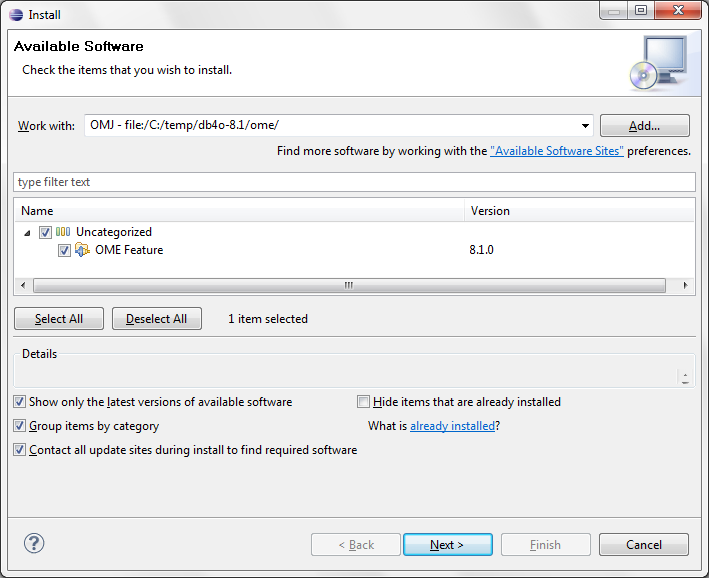
\includegraphics[width=\maxwidth]{images/tut-omj-installation.png}
\end{center}
\section*{Using the Object Manager}

To use the object manager we first open the OME perspective ('Window'-\textgreater{}'Open Perspective'-\textgreater{}'Other...'. Then we can open a db4o database.

After connecting we see a list of stored classes on the right. Below that we can inspect a stored class and see it details.

To query the database we drag and drop the fields we're interested in to the query builder. Then we change the condition and values on that query and run it.

\begin{center}
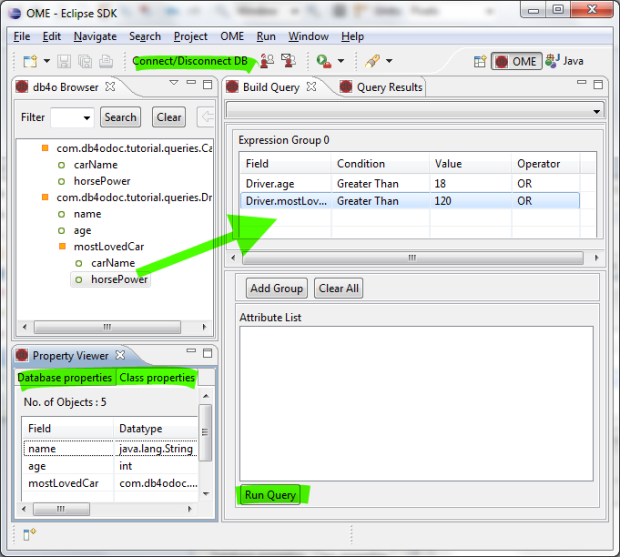
\includegraphics[width=\maxwidth]{images/tut-ome-overview.png}
\end{center}
On the result page we can select the different objects and inspect their values. We also can change values of objects and then store the data.

\begin{center}
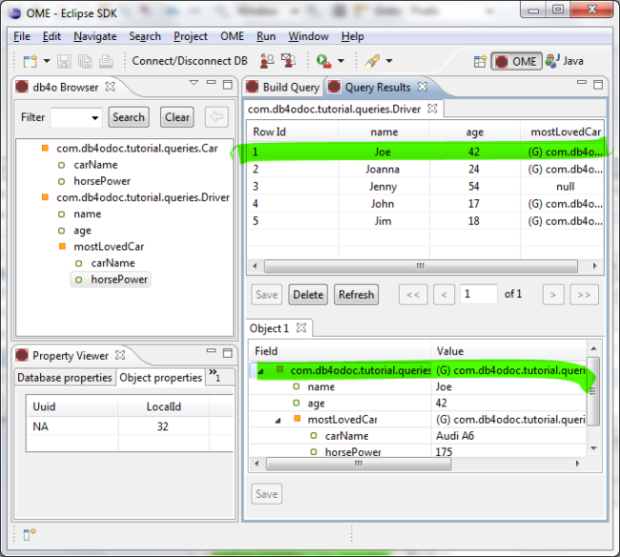
\includegraphics[width=\maxwidth]{images/tut-omj-result.png}
\end{center}

% Converted from reference/DB4OTutorial (MadCap Flare, Java target)

\chapter{Community}
\label{tut:db4ocommunity}

That's it for the tutorial and you now can go wild with db4o. You also can participate in the db4o community and help to improve db4o. The main community website for db4o is \href{http://community.versant.com/}{http://community.versant.com}. There you can find forums, blog posts, additional resources and the newest db4o releases.

\section{Forums}
\label{tut:db4ocommunity:forums}

The best place to ask questions about db4o, discuss and make suggestions is the db4o forum. You can find the db4o forums here: \href{http://community.versant.com/Forums.aspx}{http://community.versant.com/Forums.aspx}

\section{Additional Resources}
\label{tut:db4ocommunity:resources}

To stay informed about new features, community activity and other news subscribe to the different db4o blogs: \href{http://community.versant.com/Blogs.aspx}{http://community.versant.com/Blogs.aspx.}

Or follow us on Twitter: \href{http://twitter.com/db4objects}{http://twitter.com/db4objects}

\section{Report Bugs}
\label{tut:db4ocommunity:bugrepors}

Software contains bugs and so does db4o. If you find bugs please report them to us. In case you're not sure if you found a bug, you maybe want to discuss your issue first on the \href{http://community.versant.com/Forums.aspx}{db4o forum}. As soon as you're sure that you've found a bug please report it on \href{http://tracker.db4o.com/}{our bug-tracking system}. The login is the same as in the db4o forums.

When possible include a small test program which reproduces the issue. A test case avoids confusion and effort to reproduce the bug.


% Converted from reference/DB4OTutorial (MadCap Flare, Java target)

\chapter{Contact}
\label{tut:contact}

db4o was developed by Versant Corporation, which no longer develops, sells or supports it. The original company websites, forums, blogs and bug tracker no longer exist.

This edition of db4o is maintained at \href{https://github.com/blakemcbride/db4o}{\nolinkurl{github.com/blakemcbride/db4o}}. The repository contains the source code, the build instructions (\href{https://github.com/blakemcbride/db4o/blob/master/BUILD.md}{\nolinkurl{BUILD.md}}) and this manual.

\part{Reference}
% Converted from reference/DB4OFlare (MadCap Flare, Java target)

\chapter{Introduction}
\label{ref:welcome}

\href{http://community.versant.com/}{db4o} is an object database management system developed and distributed by \href{http://www.versant.com/}{Versant Corporation}. db4o is an open-source product and is available under \hyperref[ref:license]{dual license.} (p.~\pageref{ref:license})

\section*{Overview}

\begin{itemize}
\item To install db4o read the \hyperref[ref:basics-getting-started]{getting started manual} (p.~\pageref{ref:basics-getting-started}).
\item For information about the database operations with db4o read about \hyperref[ref:basics-object-container]{the basic operations} (p.~\pageref{ref:basics-object-container}).  Use \hyperref[ref:basics-querying-native-queries]{native queries} (p.~\pageref{ref:basics-querying-native-queries}) to query for object in your database.  There are also other alternative query methods: \hyperref[ref:basics-querying-query-by-example]{query by example} (p.~\pageref{ref:basics-querying-query-by-example}) and \hyperref[ref:basics-querying-soda-query]{SODA} (p.~\pageref{ref:basics-querying-soda-query}).
\item Take a look at basic db4o concepts like \hyperref[ref:basics-acid-and-transactions-db4o-tx-basics]{transaction handling} (p.~\pageref{ref:basics-acid-and-transactions-db4o-tx-basics}) and \hyperref[ref:basics-acid-and-transactions]{ACID properties} (p.~\pageref{ref:basics-acid-and-transactions}) and \hyperref[ref:basics-identity-concept]{object identity} (p.~\pageref{ref:basics-identity-concept}) .
\item To get an idea when db4o loads object into memory read about \hyperref[ref:basics-activation]{the activation concept} (p.~\pageref{ref:basics-activation}). And learn you \hyperref[ref:basics-update-concept]{update} (p.~\pageref{ref:basics-update-concept}) and \hyperref[ref:basics-delete-behavior]{delete} (p.~\pageref{ref:basics-delete-behavior}) objects with db4o.
\item For good query performance you \hyperref[ref:basics-indexing]{should create indexes} (p.~\pageref{ref:basics-indexing}).
\item Read about all the db4o \hyperref[ref:configuration]{configuration options} (p.~\pageref{ref:configuration}) available to you. How you can change the \hyperref[ref:configuration-file-storage]{storage system} (p.~\pageref{ref:configuration-file-storage}), the \hyperref[ref:configuration-common-activation-depth]{activation} (p.~\pageref{ref:configuration-common-activation-depth}) and \hyperref[ref:configuration-common-update-depth]{update} (p.~\pageref{ref:configuration-common-update-depth}) depth and how you can configure an \hyperref[ref:configuration-objectclass-configuration]{individual class} (p.~\pageref{ref:configuration-objectclass-configuration}).
\item db4o also support a \hyperref[ref:client-server]{client server} (p.~\pageref{ref:client-server}) mode.
\item Take a look at \hyperref[ref:advanced-topics]{advanced features} (p.~\pageref{ref:advanced-topics}) like \hyperref[ref:advanced-topics-session-containers]{session containers} (p.~\pageref{ref:advanced-topics-session-containers}), \hyperref[ref:advanced-topics-unique-constraints]{unique constrains} (p.~\pageref{ref:advanced-topics-unique-constraints}), \hyperref[ref:advanced-topics-backup]{backups} (p.~\pageref{ref:advanced-topics-backup}), \hyperref[ref:advanced-topics-ids-and-uuids]{db4o ids and UUIDs} (p.~\pageref{ref:advanced-topics-ids-and-uuids}) and \hyperref[ref:advanced-topics-db4o-meta-information]{meta-information} (p.~\pageref{ref:advanced-topics-db4o-meta-information}).
\item \hyperref[ref:advanced-topics-callbacks]{Callbacks} (p.~\pageref{ref:advanced-topics-callbacks}) allow you to take action on certain database events.
\item You should \hyperref[ref:advanced-topics-defragment]{defragment} (p.~\pageref{ref:advanced-topics-defragment}) the database from time to time for the best performance.
\item Read about the \hyperref[ref:advanced-topics-refactoring-and-schema-evolution]{refactoring support} (p.~\pageref{ref:advanced-topics-refactoring-and-schema-evolution}) in db4o.
\item Take a look at the best \hyperref[ref:best-practises]{practices} (p.~\pageref{ref:best-practises}) and \hyperref[ref:usage-pitfalls]{pitfalls} (p.~\pageref{ref:usage-pitfalls}) for db4o.
\item db4o supports on many platforms and those have some \hyperref[ref:platform-specific-issues]{platform specific limitations} (p.~\pageref{ref:platform-specific-issues}). Like the pitfalls in a \hyperref[ref:platform-specific-issues-web-environment]{web environment} (p.~\pageref{ref:platform-specific-issues-web-environment}), and  \hyperref[ref:platform-specific-issues-android]{Android} (p.~\pageref{ref:platform-specific-issues-android}).
\item For replication between db4o, VOD and Hibernate, read the \hyperref[drs:welcome]{db4o Replication System documentation} (p.~\pageref{drs:welcome}).
\end{itemize}

\section*{Join The db4o Community}

Join the \href{http://community.versant.com/}{db4o community} for additional help, tips and tricks. Ask for help in the \href{http://community.versant.com/Forums.aspx}{db4o forums} at any time. If you want to stay informed, subscribe to our \href{http://community.versant.com/Blogs.aspx}{blogs}.


% Converted from reference/DB4OFlare (MadCap Flare, Java target)

\chapter{Product Philosophy}
\label{ref:product-philosophy}

db4o was originally developed by Versant Corporation, a developer of object database technology based in Redwood City, California. Versant has since discontinued db4o. It remains open source and is now maintained at \href{https://github.com/blakemcbride/db4o}{\nolinkurl{github.com/blakemcbride/db4o}}.

Versant's commercial object database technology, targeting extreme scale systems, is powering some of the world's most demanding applications for fortune 1000 companies in industries including:

\begin{itemize}
\item Telecommunications: Alcatel-Lucent, Deutsche Telecom, France Telecom, Ericsson, NEC, Nortel, Orange, Samsung, and more.
\item Finance: Financial Times, New York Stock Exchange, Dow Jones, Reuters, London Clearing House, Bank of America, and more,
\item Transportation: Sabre, GE Railways, BNS Railways, Galileo, and more.
\item Defense: Raytheon, Northrop Grumman, Lockheed, and more.
\item BioInformatics: Mayo Clinic, St. Jude medical, Eidogen, Science Factory, and more.
\end{itemize}

db4o has users and customers coming from 170 different countries, from Albania to Zimbabwe, and ranging from world class leaders like Boeing, Bosch, Intel, Ricoh and Seagate to a wide range of highly innovative start-up companies.

It is Versant's and the db4o team's mission to give developers a choice differentiated from relational approaches when it comes to object persistence and thus make their life a lot easier. There is no mapping! No mapping annotations or XML mapping meta data. The db4o database is designed to be a universal, affordable product platform that is easy to learn and use. Versant's open source dual-license business model combines the power of an open source development community with servicing commercial customers' needs for a predictable product roadmap, indemnification, single point of contact and full tech support with fast response times. For those requiring the super scale database capabilities, you can find the same easy to learn and implement solution in Versant's commercial products which have been in development for over a decade. This technology is also far more affordable that traditional relational database systems such as Oracle, Sybase, SQL Server, etc and to boot users also enjoy overall reductions in system footprints by as much as 50\% due to less indexing data, simpler design, zero mapping.

\section{Data Persistence}
\label{ref:product-philosophy-data-persistence}

Software programs using different data persistence technologies are an integral part of contemporary informational space. More than often such systems are implemented with the help of object-oriented programming language (Java, C\#, etc.) and a relational database management system (Oracle, MySQL, etc.). This implementation originally contains a mismatch between relational and object worlds, which is often called object/relational impedance mismatch. The essence of the problem is in the way the systems are designed. Object systems consist of objects and are characterized by identity, state, behavior, encapsulation. The relational model consists of tables, columns, rows and foreign keys and is described by relations, attributes and tuples.

The object-relational mismatch has become enormously significant with the total adoption of OO technology. This resulted in the rapid development of object-relational mappers (ORM), such as Hibernate, EclipseLink or Entity Framework. This solution "cures" the symptoms of the object relational mismatch by adding a layer into the software stack that automates the tedious task of linking objects to tables. However, this approach creates a huge drain on system performance, drives up software complexity and increases the burden on software maintenance, thus resulting in higher cost of ownership. While the mapper solution may be feasible in large, administered datacenter environments, it is prohibitive in distributed and zero-administration architectures such as those required for embedded databases in client software, mobile devices, middleware or real-time systems.

Significant side effects of the object relational mismatch manifest themselves in unnecessary system overhead with bloated footprints and runtime performance issues. Of course, there is also overall time to market delays due to poor developer productivity. The overhead still exists in ORM because under the covers, the runtime is still query driven. And, despite improvements in productivity for developers, incremental changes to your object models reek havoc during ORM schema evolution pitfalls. The more complicated your models are, the more problematic keeping changes in sync with the internal mapping.

Primary performance issues come from the fact that despite being called a "relational database", an RDBMS does not store direct relations. Relations are resolved at runtime by performing set based operations on primary-foreign key pairs. This means the application has to constantly re-discover data relationships at runtime resulting in immense CPU consumption for something that should be an inherent part of your application model. Further, because discovering these relations over and over again requires continual access to index structures and data to perform the set operations, contention is much higher within database internals leading to poor scalability of individual database processes.

Further, lack of direct storage of relations cause the application design to become query driven instead of object modeling driven. Using an object database, the relations are a fundamental part of the storage architecture. So, application design is model driven. You do not have to suffer any performance overhead for discovering an M-M relationship. The relationships are just there and immediately accessible to the requesting thread. This makes the internal structures much simpler and therefore less contention exists with data requests being isolated to data of interest instead of leveraging indexes or sequential scans. The result, individual processes become more scalable under concurrency.

Technology is ever changing and today there is a whole world of object database experts in the software community. Anyone who is an expert in ORM technology is an expert in object database technology. All of the concepts found in object life cycle management within ORM technologies were invented by the object database community in the early 90's. All of the tuning concepts of closure, fetch configurations, value vs reference types, light weight transactions - are concepts created by and applicable to object database technologies. Now with the growing popularity of object based design and the proliferation of ORM tools, thousands of developers are becoming experts in the object database API.

\section{OODBMS}
\label{ref:product-philosophy-oodbms}

The emergence of distributed data architectures - in networks, on clients and embedded in "smart" products such as cars or medical devices - is causing companies in an array of industries to look beyond traditional RDBMS technology and ORM for an improved way to deal with object persistence.

They are searching for a solution that can handle an enormous number of often complex objects, offer powerful replication and query capabilities, reduce development and maintenance costs and require minimum to zero administration overhead.

These requirements can be fulfilled by using an Object Oriented Database Management System (OODBMS). OODBMS provides an ideal match with object oriented environments like Java and .NET reducing the cost of development, support and versioning and hence overall system costs.

Using OODBMS in software projects also better supports modern Agile software engineering practices like:

\begin{itemize}
\item Continuous refactoring.
\item Agile modeling.
\item Continuous regression testing.
\item Configuration management.
\item Developer "sandboxes".
\end{itemize}

For more information about OODBMS technology refer to the \href{http://www.odbms.org/}{ODBMS.ORG website}.

\section{db4o Position}
\label{ref:product-philosophy-db4o-position}

The db4o database came to the market in 2004 with a goal to become the mainstream persistence architecture for embedded applications (in which the database is invisible to the end user) in general, and for mobile and embedded devices running on Java or .NET, in particular. Versant's vision for db4o is to become the affordable, dominant, open source persistence solution of object oriented developers of Java and .NET. In a very short time, the db4o team has achieved mainstream adoption with a fast growing user community currently boasting over 60,000 members. Community adoption is continually driven by db4o's efficient innovative technology, native queries, deployment in Java and .NET and its open source dual licensing business model.

The target environments for db4o are persistence architectures where there is no database administrator present and no RDBMS legacy, i.e. primarily on equipment, mobile and desktop clients, and in the middleware. Typical industries of db4o customers include transportation, communication, automation, medical sciences, industrial, consumer and financial applications, among many others.

Existing customers range from world-class leaders like Boeing, Bosch, Intel, Ricoh, and Seagate to a broad range of highly innovative start-up companies - in the Americas, EMEA, and Asia-Pacific.

As a client-side, embeddable database, db4o is particularly suited to be deployed in devices with embedded software.

\subsection*{Open Source}

db4o is open source, available under the \hyperref[ref:license]{GNU General Public License} (p.~\pageref{ref:license}). Versant originally offered it under a dual license model, as pioneered by MySQL: the GPL and the db4o Opensource Compatibility License (dOCL) for open source projects, and a commercial license for embedding db4o in for-profit products. The dOCL and the commercial license are no longer offered.

\subsection*{Success Drivers}

Open Source platform usage is one of the key factors of db4o success. db4o's openness attracted a vast (60,000 and counting) community of users and contributors. Through the community support db4o gets broad and immediate testing, receives constructive suggestions (from the users actually looking into the code) and invaluable peer exchange of experiences - positive and negative.

Another factor to db4o success is the technology used. As a new-generation object database, native to both Java and .NET, db4o eliminates the traditional trade-off between performance and object-orientation. Recent PolePosition benchmark results show that db4o outperforms object-relational mappers by orders of magnitude, up to 44x in use cases with complex object models.

db4o uniquely offers object persistence with zero-administration, object-oriented querying, replication and browsing capabilities, and a small footprint. Its single library (JAR/DLL) is easily deployed and runs in the same memory process as the application, making it a fully integrated and tunable portion of the developers application.

Customers, analysts, and experts agree that the db4o object database is one of the world's best and most popular choices, because it stores and retrieves objects natively and not only eliminates the overhead and resource consumption of an ORM, but also greatly reduces the product development and maintenance costs, resulting in a lean, fast and easily integratable into an OO development environment persistence solution, far superior in many cases to that of any RDBMS.

\subsection{db4o Applications}
\label{ref:product-philosophy-db4o-applications}

db4o can be used in a wide range of production and educational software. The primary focus is on embedded usage, like mobile systems (phones and handhelds), device electronics (printers, cars, robots), SCADA systems etc. The following table provides many (but not all) possible implementations with an explanations of the benefits of db4o in the selected environment:

{\small
\begin{longtable}{|p{\dimexpr(\linewidth-3\arrayrulewidth)*1/2-2\tabcolsep\relax}|p{\dimexpr(\linewidth-3\arrayrulewidth)*1/2-2\tabcolsep\relax}|}
\hline
\textbf{Environment} & \textbf{Benefits} \\ \hline
Educational systems & One-line persistence, Object-oriented model, intuitive programming interface make db4o an ideal educational tool. It is easy to use and it provides a meaningful example of object-oriented world. It is also native to most widely used OO languages: Java and .NET \\ \hline
Prototypes & Using db4o to build a prototype system is much quicker than using an RDBMS. In case of db4o you do not need to create a data model. Further there is no need to map your object model to the database. The general persistence mechanism is almost transparent and requires minimum effort to adapt to. Automatic refactoring allows rapid change of classes without the necessity to update the database. \\ \hline
SCADA & Using db4o in SCADA systems allows to achieve high performance in caching and replay of the events. Another benefit is a small footprint and easy integration with Java and .NET programming languages. db4o can also be run as a memory database, providing better performance though minimizing disk access. \\ \hline
Mobile applications & Mobile applications can benefit from in-process database, which requires zero-administration. Synchronization with the main server can be done with the help of dRS. Automatic refactoring can be another valuable factor, which allows to skip the job of updating the databases when a new version of object model is implemented. \\ \hline
Device applications & Device applications enjoy the same benefits as Mobile applications. In addition, smaller footprints can be achieved by using the minimal Micro edition. \\ \hline
Open-source software & GPL. Native to Java and .NET. Easily integrates with any Java and .NET open-source products. \\ \hline
Web-applications & open-source, reporting support from several Java open-source reporting frameworks and .NET reporting API \\ \hline
\end{longtable}}

However, other applications might not be well suited for db4o.

For example, in situations where you have increasing amounts of data ( over 10 Gigabytes ) and high concurrency ( over 20 concurrent users/processes ) along with your complex models. In these cases, a larger database system, such as the Versant object database, is likely a more appropriate choice. Versant's customer applications span a wide range of use including those exhibiting 1000's of current transactions ( 100's of thousands of concurrent tx per second ) to 100's of gigabytes with some Versant customers in the 25T+ sized database.

Another case is when you have simple and flat data model, primarily used for reporting. Simple table-like models of tuple records may be better supported by an RDBMS. In this case, adhoc data access would be more important to your application than well defined use cases using an object model. Typically this is complimented with the need let your users to be able to grab one of the plethora of commercial tools to poke at the database in an adhoc fashion.

\subsection{Scalability}
\label{ref:product-philosophy-scalability}

db4o is intended for embedded use with smaller databases around 2-16 GByte and at maximum 256 GByte. As a general rule, if you expect your database to grow beyond 16 gigabytes, you should look at a larger database system.

db4o is explicitly single-threaded. Concurrent accesses will be synchronized against a global database lock. That means db4o cannot deal with a highly concurrent access, since it blocks on all operations. When you expect a high load and concurrent access, then you should consider a larger database system.

If you want to make sure that your application can grow and scale with db4o database you may take the following steps:

\begin{itemize}
\item Write performance tests to accommodate for performance requirements of the growing application. Especially look that you capture the complexity of the model and don't use a simplified flat data model.
\item Also check that you can the throughput you need with concurrent access.
\end{itemize}

\section{Why Choose db4o}
\label{ref:product-philosophy-why-choose-db4o}

There are many advantages of using "native" object technology over RDBMS or RDBMS paired with an OR mapper, and these technological advantages significantly impact an organization's competitiveness and bottom line.

First, object databases not only simplify development by eliminating the resource-consuming OR-mismatch entirely, but they also foster more sophisticated and differentiated product development through gains in flexibility and productivity brought on by "true" object-orientation.

Second, with an object database, the object schema is the same as the data model. Developers can easier update their models to meet changing requirements, or for purposes of debugging or refactoring. db4o lets developers work with object structures almost as if they were "in-memory"' structures. Little additional coding is required to manage object persistence. As a result, companies can add new features to their products faster to stay ahead of the competition.

Third, developers can now use object-oriented and entirely native approaches when it comes to querying, since db4o was the first in the industry to provide Native Queries (NQ) with its Version 5.0 launched in November 2005 and since introduction of LINQ in .NET version 3.5. Db4o Native Queries provide an API that uses the programming languages Java or .NET to access the database. No time is spent on learning a separate data manipulation or query language. Unlike incumbent, string-based, non-native APIs (such as SQL, OQL, JDOQL and others) Native Queries and LINQ are 100\% type-safe, 100\% refactorable and 100\% object-oriented, boosting developer productivity by up to 30\%. In addition, the sophisticated modern programming development environments can be used to simplify the development and maintenance work even further.

Fourth, db4o's ground-breaking object-oriented replication technology solves problems arising from distributed data architectures. Partially connected devices need to efficiently replicate data with peers or servers. The challenge lies in the creation of "smart" conflict resolution algorithms, when redundant data sets are simultaneously modified and need to be merged. With db4o's OO approach, developers can build smarter and easier synchronization conflict resolution and embed the necessary business logic into the data layer, rather than into the middle-tier or application layer. This creates "smart" objects that can be stored in a distributed fashion, but easily consolidated, as the object itself knows how to resolve synchronization conflicts. It also enables db4o solution on a client to synchronize data with an RDBMS backend server.

As a result, developers can now more consistently persist data on distributed, partially connected clients than ever before, while decreasing bandwidth requirements and increasing the responsiveness and reach of their mobile solutions or smart devices to make products more competitive in the marketplace.

Fifth, db4o also allows for more complex object models than its relational or non-native counterparts do. As the persistence requirements become more complex, db4o's unique design easily handles (or absorbs) the added complexity, so developers can continue to work as though new complexity were never introduced. Complexity means not only taller object trees and extensive use of inheritance, but also dynamically evolving object models, most extremely if development is taking place under runtime conditions (which makes db4o a leading choice for biotech simulation software, for instance). db4o could be referred to as "agnostic to complexity," because it can automatically handle changes to the data model, without requiring extra work. No type or amount of complexity will change its behavior or restrain its capabilities, as is the case with RDBMS or non-native technology. With db4o breaking through this complexity, developers are able to write more user friendly and business-appropriate software components without incurring such high costs and modify them as needed, throughout the life cycle of the product with the same low cost.

In sum, db4o's native, object oriented architecture enables its users to build more competitive products with faster update cycles, more natural object models that match more realistically their use cases, and more distributed data architectures to increase the reach of products. db4o is clearly more flexible and powerful for embedded DB applications than any non-native OODBMS or RDBMS technologies available.


% Converted from reference/DB4OFlare (MadCap Flare, Java target)

\chapter{Basics Operations \& Concepts}
\label{ref:basics}

This topic gives you an overview of the most important and basic features of db4o. First add db4o to your project. db4o doesn't need a complex setup. It's just a library which you can add to your project. \hyperref[ref:basics-getting-started]{See "Getting Started"} (p.~\pageref{ref:basics-getting-started})

\section*{Basic Operations}

The basic operations are unsurprisingly, storing, updating, querying and deleting objects. \hyperref[ref:basics-object-container]{See "The Basic Operations"} (p.~\pageref{ref:basics-object-container})

\begin{lstlisting}
ObjectContainer container = Db4oEmbedded.openFile("databaseFile.db4o");
try {
    // store a new pilot
    Pilot pilot = new Pilot("Joe");
    container.store(pilot);

    // query for pilots
    List<Pilot> pilots = container.query(new Predicate<Pilot>() {
        @Override
        public boolean match(Pilot pilot) {
            return pilot.getName().startsWith("Jo");
        }
    });

    // update pilot
    Pilot toUpdate = pilots.get(0);
    toUpdate.setName("New Name");
    container.store(toUpdate);

    // delete pilot
    container.delete(toUpdate);
} finally {
    container.close();
}
\end{lstlisting}

{\small\itshape Db4oBasics.java: The basic operations\par}
\medskip

For more information about queries: \hyperref[ref:basics-querying]{See "Querying"} (p.~\pageref{ref:basics-querying})

\section*{Basic Concepts}

There are some basic concepts which are used in db4o. Understanding them helps you to understand how db4o behaves. Some behaviors are common behaviors which you expect from a database, like transactions and ACID properties. \hyperref[ref:basics-acid-and-transactions]{See "ACID Properties And Transactions"} (p.~\pageref{ref:basics-acid-and-transactions})

db4o manages objects by identity. This means db4o doesn't need additional id-field on your object. \hyperref[ref:basics-identity-concept]{See "Identity Concept"} (p.~\pageref{ref:basics-identity-concept})

Other concepts are more unique to db4o, like the activation concept, which controls which objects are loaded from the storage to memory. \hyperref[ref:basics-activation]{See "Activation Concept"} (p.~\pageref{ref:basics-activation}). The same principals are also applied when updating (\hyperref[ref:basics-update-concept]{See "Update Concept"} (p.~\pageref{ref:basics-update-concept})  ) or deletion objects (\hyperref[ref:basics-delete-behavior]{See "Delete Behavior")} (p.~\pageref{ref:basics-delete-behavior})

\section{Getting Started}
\label{ref:basics-getting-started}

You can start using db4o within a few minutes following these few steps.

\subsection*{1. Get db4o}

db4o is maintained at \href{https://github.com/blakemcbride/db4o}{\nolinkurl{github.com/blakemcbride/db4o}}. Clone or download the repository; it contains the source code, the build and this manual.

\subsection*{2. Build db4o}

Build the jars as described in \href{https://github.com/blakemcbride/db4o/blob/master/BUILD.md}{\nolinkurl{BUILD.md}}. You need JDK 17 or newer and nothing else:

\begin{lstlisting}
./bld jar          # Linux, macOS
bld.cmd jar        # Windows
\end{lstlisting}

The jars are written to the target directory. \texttt{./bld javadoc} builds the API documentation into target/javadoc.

\subsection*{3. Adding db4o To Your Project}

The core of db4o is the single db4o-8.1-core.jar and has no additional dependencies. The other jars provide additional functionality \hyperref[ref:dependency-overview]{See "Dependency Overview".} (p.~\pageref{ref:dependency-overview}). You can also use db4o-8.1-all.jar, which includes every db4o feature.

To use db4o in your project you only need to add the required jars to your project and then you're ready to go.

Here is how to do this with Eclipse:

\begin{itemize}
\item Copy the db4o-*.jar to your projects library folder. If you don't have a library-folder yet, create one under your project. For example a folder called 'lib'.
\item Right-click on your project in the Package Explorer and choose "Refresh".
\item Right-click on your project in the Package Explorer again and choose "Properties".
\item Select "Java Build Path" in the tree view on the left.
\item Select the "Libraries" tabpage.
\item Click "Add JARs".
\item Your library folder should appear below your project. Choose the db4o-*.jars in this folder.
\item Confirm the changes.
\item Expand "Referenced Libraries" branch of your project in Package Explorer.
\item Select db4o-* library, right-click and open "Properties".
\item Select Javadoc Location in the list and browse to the target/javadoc folder of your db4o build.
\end{itemize}

\subsection*{4. Ready To Go}

That's it, now you're ready to go and can use db4o in your project.

\section{The Basic Operations}
\label{ref:basics-object-container}

The object container is the door to the database access. It's the starting point for all database operations.

\subsection{Access The Database}
\label{ref:basics-object-container:accessingdb}

The object container is the interface for accessing the database. To open the database you pass the file-name to the object container factory. Normally you should open an object container when the application starts and close it when it is shuts down.

\begin{lstlisting}
ObjectContainer container = Db4oEmbedded.openFile("databaseFile.db4o");
try {
    // use the object container
} finally {
    container.close();
}
\end{lstlisting}

{\small\itshape Db4oBasics.java: Open the object container to use the database\par}
\medskip

\subsection{Store Objects}
\label{ref:basics-object-container:storingobject}

Storing a object with db4o is extremely easy. Open the object container and pass your object to the store method and db4o will do the rest. There's no mapping required. db4o will read the class meta data, the read the object values with reflection and store the data.

\begin{lstlisting}
ObjectContainer container = Db4oEmbedded.openFile("databaseFile.db4o");
try {
    Pilot pilot = new Pilot("Joe");
    container.store(pilot);
} finally {
    container.close();
}
\end{lstlisting}

{\small\itshape Db4oBasics.java: Store an object\par}
\medskip

\subsection{Query The Database}
\label{ref:basics-object-container:queries}

Querying for objects is also easy. There are different query interfaces available with different benefits. \hyperref[ref:basics-querying]{See "Querying"} (p.~\pageref{ref:basics-querying})

The most natural query method is using \hyperref[ref:basics-querying-native-queries]{native queries} (p.~\pageref{ref:basics-querying-native-queries}). Basically you just pass in a instance of a predicate, which filters the objects out you want.

\begin{lstlisting}
ObjectContainer container = Db4oEmbedded.openFile("databaseFile.db4o");
try {
    List<Pilot> pilots = container.query(new Predicate<Pilot>() {
        public boolean match(Pilot o) {
            return o.getName().equals("Joe");
        }
    });
    for (Pilot pilot : pilots) {
        System.out.println(pilot.getName());
    }
} finally {
    container.close();
}
\end{lstlisting}

{\small\itshape Db4oBasics.java: Query for objects\par}
\medskip

\subsection{Update Objects}
\label{ref:basics-object-container:updateobjects}

Updating objects is also easy. First you query for the object which you want to update. Then you change the object and store it again in the database.

\begin{lstlisting}
ObjectContainer container = Db4oEmbedded.openFile("databaseFile.db4o");
try {
    List<Pilot> pilots = container.query(new Predicate<Pilot>() {
        public boolean match(Pilot o) {
            return o.getName().equals("Joe");
        }
    });
    Pilot aPilot = pilots.get(0);
    aPilot.setName("New Name");
    // update the pilot
    container.store(aPilot);
} finally {
    container.close();
}
\end{lstlisting}

{\small\itshape Db4oBasics.java: Update a pilot\par}
\medskip

\subsection{Delete Objects}
\label{ref:basics-object-container:deleteobjects}

Use the delete-operation to delete objects.

\begin{lstlisting}
ObjectContainer container = Db4oEmbedded.openFile("databaseFile.db4o");
try {
    List<Pilot> pilots = container.query(new Predicate<Pilot>() {
        public boolean match(Pilot o) {
            return o.getName().equals("Joe");
        }
    });
    Pilot aPilot = pilots.get(0);
    container.delete(aPilot);
} finally {
    container.close();
}
\end{lstlisting}

{\small\itshape Db4oBasics.java: Delete a object\par}
\medskip

\section{Querying}
\label{ref:basics-querying}

db4o supports different query mechanisms.

\hyperref[ref:basics-querying-native-queries]{Native Queries} (p.~\pageref{ref:basics-querying-native-queries}) is the main db4o query interface, recommended for general use.

\hyperref[ref:basics-querying-query-by-example]{Queries-By-Example} (p.~\pageref{ref:basics-querying-query-by-example}) are appropriate as a quick start for users who are still acclimating to storing and retrieving objects with db4o, but they are quite restrictive in functionality.

The \hyperref[ref:basics-querying-soda-query]{SODA Query} (p.~\pageref{ref:basics-querying-soda-query}) is the underlying internal API. It is provided for backward compatibility and it can be useful for dynamic generation of queries, where Native Queries are too strongly typed. There may be queries that will execute faster in SODA style, so it can be used to tune applications. You can also run snippets of custom query code as part of the SODA query,

Of course, you can mix these strategies as needed.

\subsection{Native Queries}
\label{ref:basics-querying-native-queries}

Wouldn't it be nice to write queries in the programming language that you are using? Wouldn't it be nice if all your query code was 100\% typesafe, 100\% compile-time checked and 100\% refactorable? Wouldn't it be nice if the full power of object-orientation could be used by calling methods from within queries?

Native queries allow you do to this. They bring you a nice query interface which doesn't rely on string literals. Because native queries simply use the semantics of your programming language, they are perfectly standardized and a safe choice for the future.

Native Queries are available for all platforms supported by db4o.

\subsubsection*{Principle}

Native Queries provide the ability to run one or more lines of code against all instances of a class. Native query expressions should return true to mark specific instances as part of the result set. db4o will attempt to \hyperref[ref:basics-querying-native-queries-native-query-optimization]{optimize native query} (p.~\pageref{ref:basics-querying-native-queries-native-query-optimization}) expressions where possible and use \hyperref[ref:basics-querying-soda-query]{internal query processor} (p.~\pageref{ref:basics-querying-soda-query}) to run them against indexes and without instantiating actual objects.

\subsubsection*{Dependencies}

For a good native query performance you need to add these jars to your project:db4o-8.1-nqopt.jar, db4o-8.1-instrumentation.jar, db4o-8.1-bloat.jar. \hyperref[ref:dependency-overview]{See "Dependency Overview"} (p.~\pageref{ref:dependency-overview})

\subsubsection*{Simple Example}

Let's look at how a simple native query will look like. See also a collection of example queries.

\begin{lstlisting}
ObjectSet<Pilot> result = container.query(new Predicate<Pilot>() {
    @Override
    public boolean match(Pilot pilot) {
        return pilot.getName().equals("John");
    }
});
\end{lstlisting}

{\small\itshape NativeQueryExamples.java: Check for equality of the name\par}
\medskip

\subsubsection*{Native Query Performance}

There's one drawback of native queries: Under the hood db4o tries to analyze native queries to convert them to \hyperref[ref:basics-querying-soda-query]{SODA} (p.~\pageref{ref:basics-querying-soda-query}). This is not possible for all queries. For some queries it is very difficult to analyze the flowgraph. In this case db4o will have to instantiate some of the persistent objects to actually run the native query code. db4o will try to analyze parts of native query expressions to keep object instantiation to the minimum.

The current state of the query optimization process is detailed in the chapter on \hyperref[ref:basics-querying-native-queries-native-query-optimization]{Native Query Optimization} (p.~\pageref{ref:basics-querying-native-queries-native-query-optimization})

\subsubsection*{Lazy Loaded Result Set}

db4o always returns lazy loaded result sets. That means the object container needs to stay open as long as you are using the result set. If you want use the result of a query after the object container has been closed, you need to copy the query result into a new collection first.

\subsubsection{Native Query Examples}
\label{ref:basics-querying-native-queries-native-query-examples}

Here's a collection of native query examples. These queries assume that there's a Pilot class with a name and age and a Car class with a pilot and name.

\paragraph{Equality}
\label{ref:basics-querying-native-queries-native-query-examples:equality}

This query shows you how compare a getter/setter for equality. In this example we compare the name of a person.

\begin{lstlisting}
ObjectSet<Pilot> result = container.query(new Predicate<Pilot>() {
    @Override
    public boolean match(Pilot pilot) {
        return pilot.getName().equals("John");
    }
});
\end{lstlisting}

{\small\itshape NativeQueryExamples.java: Check for equality of the name\par}
\medskip

\paragraph{Comparison}
\label{ref:basics-querying-native-queries-native-query-examples:comparison}

You can compare values with the usual comparison operators.

\begin{lstlisting}
ObjectSet<Pilot> result = container.query(new Predicate<Pilot>() {
    @Override
    public boolean match(Pilot pilot) {
        return pilot.getAge() > 18;
    }
});
\end{lstlisting}

{\small\itshape NativeQueryExamples.java: Compare values to each other\par}
\medskip

\paragraph{Query For Value Range}
\label{ref:basics-querying-native-queries-native-query-examples:valuerange}

Of course you can combine different comparisons. For example you can combine the greater and smaller than operators to check for a range of values.

\begin{lstlisting}
ObjectSet<Pilot> result = container.query(new Predicate<Pilot>() {
    @Override
    public boolean match(Pilot pilot) {
        return pilot.getAge() > 18 && pilot.getAge()<30;
    }
});
\end{lstlisting}

{\small\itshape NativeQueryExamples.java: Query for a particular rage of values\par}
\medskip

\paragraph{Combine Check With Logical Operators}
\label{ref:basics-querying-native-queries-native-query-examples:logicaloperators}

Of course you can combine a arbitrary set of conditions with logical operators.

\begin{lstlisting}
ObjectSet<Pilot> result = container.query(new Predicate<Pilot>() {
    @Override
    public boolean match(Pilot pilot) {
        return (pilot.getAge() > 18 && pilot.getAge()<30)
                || pilot.getName().equals("John");
    }
});
\end{lstlisting}

{\small\itshape NativeQueryExamples.java: Combine different comparisons with the logical operators\par}
\medskip

\paragraph{Query In Separate Class}
\label{ref:basics-querying-native-queries-native-query-examples:seperatequeryunit}

You can implement your query in a separate class  and then just us it where you need it. This is especially useful when you reuse the same query multiple times. Or you want to give your query a clear name for documentation purposes.

First write your  class :

\begin{lstlisting}
class AllJohns extends Predicate<Pilot> {
    @Override
    public boolean match(Pilot pilot) {
        return pilot.getName().equals("John");
    }
}
\end{lstlisting}

{\small\itshape AllJohns.java: Query as class\par}
\medskip

And then use it:

\begin{lstlisting}
ObjectSet<Pilot> result = container.query(new AllJohns());
\end{lstlisting}

{\small\itshape NativeQueryExamples.java: Use the predefined query\par}
\medskip

\paragraph{Arbitrary Code}
\label{ref:basics-querying-native-queries-native-query-examples:arbitrarycode}

In principal your query can contain any code and can do the most complex comparisons. However in practice the are limitations. The simple queries are \hyperref[ref:basics-querying-native-queries-native-query-optimization]{optimized and translated to SODA-queries} (p.~\pageref{ref:basics-querying-native-queries-native-query-optimization}). This is not possible for complex queries. If the query cannot be optimized, db4o will instantiate all objects and pass it to your query-object. This is a order of magnitude slower than a optimized native query and only feasible for smaller data sets.

\begin{lstlisting}
final List<Integer> allowedAges = Arrays.asList(18,20,33,55);
ObjectSet<Pilot> result = container.query(new Predicate<Pilot>() {
    @Override
    public boolean match(Pilot pilot) {
        return allowedAges.contains(pilot.getAge()) ||
               pilot.getName().toLowerCase().equals("John"); 
    }
});
\end{lstlisting}

{\small\itshape NativeQueryExamples.java: Arbitrary code\par}
\medskip

\subsubsection{Native Query Sorting}
\label{ref:basics-querying-native-queries-native-query-sorting}

Native Query syntax allows you to specify a comparator, which will be used to sort the results:

\begin{lstlisting}
final ObjectSet<Pilot> pilots = container.query(new Predicate<Pilot>() {
    @Override
    public boolean match(Pilot o) {
        return o.getAge() > 18;
    }
}, new QueryComparator<Pilot>() {
    public int compare(Pilot pilot, Pilot pilot1) {
        return pilot.getName().compareTo(pilot1.getName());
    }
});
\end{lstlisting}

{\small\itshape NativeQueriesSorting.java: Native query with sorting\par}
\medskip

\subsubsection{NQ Performance Characteristics}
\label{ref:basics-querying-native-queries-nq-performance-characteristics}

This overview shows which query operations perform well or badly on large datasets. It should give you an idea which operations can be used on large datasets and which operations can only be applied to small datasets.

Native queries are translated to SODA and therefore they share the same basic \hyperref[ref:basics-querying-soda-soda-performance-characteristics]{performance characteristics} (p.~\pageref{ref:basics-querying-soda-soda-performance-characteristics}).

\paragraph{Good Performance Characteristics}
\label{ref:basics-querying-native-queries-nq-performance-characteristics:goodperf}

For a good query performance fields which are used in a query have to be \hyperref[ref:basics-indexing]{indexed} (p.~\pageref{ref:basics-indexing}). Otherwise db4o needs to scan through all objects. With an index these operations should scale logarithmically with the amount of data. The following queries all assume that the fields are indexed.

\subparagraph*{Equals Operation on Indexed Field}

Simple equals operations on indexed fields' perform very well.

\begin{lstlisting}
final String criteria = Item.dataString(rnd.nextInt(NUMBER_OF_ITEMS));
final List<Item> result = container.query(new Predicate<Item>() {
    @Override
    public boolean match(Item o) {
        return o.getIndexedString().equals(criteria);
    }
});
\end{lstlisting}

{\small\itshape GoodPerformance.java: Equals operation\par}
\medskip

Not equals operations also do perform well. However a 'not equals' operation tends to return a large result which will slow down the query.

\begin{lstlisting}
final String criteria = Item.dataString(rnd.nextInt(NUMBER_OF_ITEMS));
final List<Item> result = container.query(new Predicate<Item>() {
    @Override
    public boolean match(Item o) {
        return !o.getIndexedString().equals(criteria);
    }
});
\end{lstlisting}

{\small\itshape GoodPerformance.java: Not equals operation\par}
\medskip

\subparagraph*{Navigation Queries on Index Field}

Queries which navigate along references are executed also efficiently, as long every field and reference is indexed.

However there's a catch to this: The reference field type has to be a concrete type. If a field type is a generic type, an interface or an object-type, then the query runs slow.

\begin{lstlisting}
final String criteria = Item.dataString(rnd.nextInt(NUMBER_OF_ITEMS));
final List<ItemHolder> result = container.query(new Predicate<ItemHolder>() {
    @Override
    public boolean match(ItemHolder o) {
        return o.getIndexedReference().getIndexedString().equals(criteria);
    }
});
\end{lstlisting}

{\small\itshape GoodPerformance.java: Navigate across object references\par}
\medskip

\subparagraph*{Reference-Queries}

Like regular equals operation, comparisons against references also have a good performance.

\begin{lstlisting}
final Item item = loadItemFromDatabase();

final List<ItemHolder> result = container.query(new Predicate<ItemHolder>() {
    @Override
    public boolean match(ItemHolder o) {
        return o.getIndexedReference()==item;
    }
});
\end{lstlisting}

{\small\itshape GoodPerformance.java: Query by reference\par}
\medskip

\subparagraph*{Comparison and Range Queries}

Comparison and range queries also perform well.

\begin{lstlisting}
final List<Item> result = container.query(new Predicate<Item>() {
    @Override
    public boolean match(Item o) {
        return o.getIndexNumber()>criteria;
    }
});
\end{lstlisting}

{\small\itshape GoodPerformance.java: Bigger than\par}
\medskip

\begin{lstlisting}
final List<Item> result = container.query(new Predicate<Item>() {
    @Override
    public boolean match(Item o) {
        return o.getIndexNumber()>biggerThanThis && o.getIndexNumber() <smallerThanThis;
    }
});
\end{lstlisting}

{\small\itshape GoodPerformance.java: In between\par}
\medskip

\subparagraph*{Date Queries}

Simple equals operations on dates are fast. However complex date comparisons are not yet optimized and run extremely slowly. For those you \hyperref[ref:basics-querying-soda-soda-performance-characteristics]{can fallback to SODA} (p.~\pageref{ref:basics-querying-soda-soda-performance-characteristics}).

\begin{lstlisting}
final List<Item> result = container.query(new Predicate<Item>() {
    @Override
    public boolean match(Item o) {
        return o.getIndexDate().equals(date);
    }
});
\end{lstlisting}

{\small\itshape GoodPerformance.java: Search for a date\par}
\medskip

\paragraph{Bad Performance Characteristics}
\label{ref:basics-querying-native-queries-nq-performance-characteristics:badperf}

Here's an overview of the query operations with bad performances characteristics. The reason is that db4o cannot utilize indexes to perform these queries. Or that the native query optimizer cannot translate the query to SODA. That means the query time grows linearly with the amount of data.

\subparagraph*{Navigation across Generic/Object/Interface Fields}

When your query navigates across a getter which type is a generic parameter, an object or interface then the performance is bad. This is a limitation of the current query system implementation.

\begin{lstlisting}
// The type of the 'indexedReference' is the generic parameter 'T'.
// Due to type type erasure that type is unknown to db4o
final List<GenericItemHolder<Item>> result = container.query(new Predicate<GenericItemHolder<Item>>() {
    @Override
    public boolean match(GenericItemHolder<Item> o) {
        return o.getIndexedReference().getIndexedString().equals(criteria);
    }
});
\end{lstlisting}

{\small\itshape BadPerformance.java: Navigation non concrete types\par}
\medskip

\subparagraph*{String Operations: Like, Contains, StartsWith, Ends With}

All string operations beside the simple equals operation cannot use indexes at the moment. Therefore all string operations like contains, like, starts with etc. run slowly. Advanced string operations are not translated to SODA and therefore run even more slowly.

\begin{lstlisting}
final List<Item> result = container.query(new Predicate<Item>() {
    @Override
    public boolean match(Item o) {
        return o.getIndexedString().contains(criteria);
    }
});
\end{lstlisting}

{\small\itshape BadPerformance.java: Contains and other string operations are slow\par}
\medskip

\subparagraph*{Date Comparisons}

The native query optimizer doesn't recognize date comparison and therefore such queries run extremely slow. You should fall \hyperref[ref:basics-querying-soda-soda-performance-characteristics]{back to SODA} (p.~\pageref{ref:basics-querying-soda-soda-performance-characteristics}) for date queries.

\begin{lstlisting}
final List<Item> result = container.query(new Predicate<Item>() {
    @Override
    public boolean match(Item o) {
        return o.getIndexDate().after(date);
    }
});
\end{lstlisting}

{\small\itshape BadPerformance.java: Slow date query\par}
\medskip

\subparagraph*{Queries on Collections / Arrays}

Any query which does contains operations on collections/arrays or navigates across a collection/array field will run slowly. The reason is that db4o cannot index collections. Furthermore the native query optimizer may doesn't recognize such a query and just loads all objects to process the query.

\begin{lstlisting}
final List<CollectionHolder> result = container.query(new Predicate<CollectionHolder>() {
    @Override
    public boolean match(CollectionHolder o) {
        return o.getItems().contains(item);
    }
});
\end{lstlisting}

{\small\itshape BadPerformance.java: Contains on collection\par}
\medskip

\paragraph*{Computation in Query Expression}

When you do a computation in a query expression, then the native query optimizer cannot optimize your query. In that case it will load all objects in order to execute your query.

\begin{lstlisting}
final List<Item> result = container.query(new Predicate<Item>() {
    @Override
    public boolean match(Item o) {
        return o.getIndexedString().equals("data for " + number);
    }
});
\end{lstlisting}

{\small\itshape BadPerformance.java: Computing expression in query\par}
\medskip

Therefore you should move any computation outside of the query. Like this:

\begin{lstlisting}
final String criteria = "data for " + number;
final List<Item> result = container.query(new Predicate<Item>() {
    @Override
    public boolean match(Item o) {
        return o.getIndexedString().equals(criteria);
    }
});
\end{lstlisting}

{\small\itshape BadPerformance.java: Fix computing expression in query\par}
\medskip

\subparagraph*{Calling Complex Methods}

Calling complex methods in native queries is a bad idea. Most of the time the native query optimizer cannot deal with a complex method and will load all objects to execute the query.

\begin{lstlisting}
final List<Item> result = container.query(new Predicate<Item>() {
    @Override
    public boolean match(Item o) {
        return o.complexMethod();
    }
});
\end{lstlisting}

{\small\itshape BadPerformance.java: Call complex method\par}
\medskip

\paragraph{Detect Slow Queries}
\label{ref:basics-querying-native-queries-nq-performance-characteristics:detect}

The best indication that a query is slow is when it cannot use any field index. Install a \hyperref[ref:advanced-topics-diagnostics]{diagnostic listener and look for the LoadedFromClassIndex} (p.~\pageref{ref:advanced-topics-diagnostics}) message. That message indicates that a query couldn't use any field index for its execution.

For native queries another indication is when the 'NativeQueryNotOptimized' or the 'NativeQueryOptimizerNotLoaded' diagnostic message occurs. Watch out \hyperref[ref:advanced-topics-diagnostics]{for those as well} (p.~\pageref{ref:advanced-topics-diagnostics}).

\subsubsection{Native Query Optimization}
\label{ref:basics-querying-native-queries-native-query-optimization}

Native queries will run out of the box in any environment. This optimization is turned on by default. Native queries will be converted to \hyperref[ref:basics-querying-soda-query]{SODA} (p.~\pageref{ref:basics-querying-soda-query}) where this is possible. This allows db4o to use indexes and optimized internal comparison algorithms. Otherwise native query may be executed by instantiating all objects, using \hyperref[ref:basics-querying-soda-soda-evaluations]{SODA evaluations} (p.~\pageref{ref:basics-querying-soda-soda-evaluations}). Naturally performance will not be as good in this case.

\paragraph*{Optimization Theory}

For Native Query the bytecode is analyzed to create an AST-like expression tree. Then the flow graph of the expression tree is analyzed and converted to a SODA query graph.

For example:

\begin{lstlisting}
ObjectSet<Pilot> result = container.query(new Predicate<Pilot>() {
    @Override
    public boolean match(Pilot pilot) {
        return pilot.getName().equals("John");
    }
});
\end{lstlisting}

{\small\itshape NativeQueryExamples.java: Check for equality of the name\par}
\medskip

First the signature of the given class is analyzed to find out the types. This is used to constrain the type in the SODA-query. Then the bytecode of query is analyzed to find out was it does. When the operations a simple and easy to convert, it will be transformed to complete SODA query:

\begin{lstlisting}
final Query query = container.query();
query.constrain(Pilot.class);
query.descend("name").constrain("John");

final ObjectSet<Object> result = query.execute();
\end{lstlisting}

{\small\itshape SodaQueryExamples.java: A simple constrain on a field\par}
\medskip

\paragraph*{Native Query Optimization}

Native query optimization on Java requires db4onqopt.jar and bloat.jar to be present in the classpath. \hyperref[ref:dependency-overview]{See "Dependency Overview"} (p.~\pageref{ref:dependency-overview}). Current optimization supports the following constructs well:

\begin{itemize}
\item Compile-time constants.
\item Simple member access.
\item Primitive comparisons.
\item The equals-method on primitive wrappers and strings.
\item The contains-,startsWith- and endsWith-method for strings.
\item Arithmetic expressions.
\item Boolean expressions.
\item Static field access.
\item Array access for static/predicate fields.
\item Arbitrary method calls on static/predicate fields (without candidate based parameters).
\item Candidate methods composed of the above.
\item Chained combinations of the above.
\end{itemize}

Note that the current implementation doesn't support polymorphism and multiline methods yet.

db4o for Java supplies three different possibilities to run optimized native queries. By default native queries are optimized at runtime when the query runs the first time. This is the most convenient way because it doesn't need any preparations.

On certain environments (embedded runtimes, older java releases) this runtime optimization doesn't work. In such cases there are two alternatives. The \hyperref[ref:basics-querying-native-queries-native-query-optimization-nq-build-time-optimisation]{compile time optimization} (p.~\pageref{ref:basics-querying-native-queries-native-query-optimization-nq-build-time-optimisation}) and the class load time optimization. \hyperref[ref:advanced-topics-enhancement-tools]{See "Enhancement Tools"} (p.~\pageref{ref:advanced-topics-enhancement-tools})

For more information on native queries optimization see \hyperref[ref:basics-querying-native-queries-native-query-optimization-monitoring-optimization]{Monitoring Optimization} (p.~\pageref{ref:basics-querying-native-queries-native-query-optimization-monitoring-optimization}).

\paragraph{Monitoring Optimization}
\label{ref:basics-querying-native-queries-native-query-optimization-monitoring-optimization}

In order to optimize native queries the bytecode is analyzed and converted into \hyperref[ref:basics-querying-soda-query]{SODA queries} (p.~\pageref{ref:basics-querying-soda-query}). This task isn't easy. If there's any doubt in the correctness of the conversion db4o won't do it. In such cases db4o falls back and instantiates all objects and runs it against the query. This is a order of magnitude slower than optimized queries. Therefore you probably want to monitor the query optimization and be warned when a query isn't optimized. This is possible with the \hyperref[ref:advanced-topics-diagnostics-diagnostic-messages-filter]{diagnostic listeners} (p.~\pageref{ref:advanced-topics-diagnostics-diagnostic-messages-filter}).

\begin{lstlisting}
configuration.common().diagnostic().addListener(new DiagnosticListener() {
    @Override
    public void onDiagnostic(Diagnostic diagnostic) {
        if(diagnostic instanceof NativeQueryNotOptimized){
            System.out.println("Query not optimized"+diagnostic);
        } else if(diagnostic instanceof NativeQueryOptimizerNotLoaded){
            System.out.println("Missing native query optimisation jars in classpath "+diagnostic);
        }
    }
});
\end{lstlisting}

{\small\itshape NativeQueryDiagnostics.java: Use diagnostics to find unoptimized queries\par}
\medskip

You can register a diagnostic listener and check for certain messages. There are two messages related to the native query optimization. The first is the \textbf{NativeQueryNotOptimized}-message. This tells you that a query couldn't be optimized. Consider simplifying the query. The second is the \textbf{NativeQueryOptimizerNotLoaded}-message. This message tells you that db4o couldn't find the libraries needed for the native query optimization. Check that you've included the jars-files \hyperref[ref:dependency-overview]{you need} (p.~\pageref{ref:dependency-overview}).

\paragraph{Native Query Optimization At Build Time}
\label{ref:basics-querying-native-queries-native-query-optimization-nq-build-time-optimisation}

If the platform you're running doesn't support optimization at runtime you can use the compile-time optimization. \hyperref[ref:advanced-topics-enhancement-tools]{See "Enhancement Tools"} (p.~\pageref{ref:advanced-topics-enhancement-tools})

\subparagraph*{Create the Enhancement Task}

First we define the enhancement-task. This task will process the jar and enhance it.

If you haven't used Ant yet, read more on the \href{http://ant.apache.org/}{official Ant website}.

\begin{lstlisting}
<target name="enhance">
    <db4o-enhance classtargetdir="${basedir}/bin"
                  jartargetdir="${basedir}/lib"
                  nq="true" ta="true"
                  collections="true">
        <classpath refid="project.classpath"/>
        <sources dir="${basedir}/bin">
            <include name="**/*.class"/>
        </sources>
    </db4o-enhance>
</target>
\end{lstlisting}

{\small\itshape simple-enhance-example.xml: Define a target which runs the task\par}
\medskip

And the execute the task after the compilation.

\begin{lstlisting}
<target name="enhance-nq">
    <db4o-enhance classtargetdir="${basedir}/bin"
                  jartargetdir="${basedir}/lib"
                  nq="true" ta="false"
                  collections="false">
        <classpath refid="project.classpath"/>
        <sources dir="${basedir}/bin">
            <include name="**/*.class"/>
        </sources>
    </db4o-enhance>
</target>
\end{lstlisting}

{\small\itshape simple-enhance-example.xml: Only enhance native queries\par}
\medskip

You can configure Eclipse to run the Ant build with each compile step. Right click on your project and choose 'Properties'. Then switch to 'Builders' and add a new one. Choose the 'Ant Builder'. On the new window choose the build-file which contains the example-code. Switch to the 'Targets'-Tab. There choose the enhance-target for the 'Auto-Build'. Now the enhancer-task will be run by Eclipse automatically. The example project above is configured this way.

Often it's practical to have all persistent classes in a separate project or compile unit. Then the enhancement script runs only for this project. This makes it easy to enhance only the classes for the persistent objects.

There are lot of possibilities to tweak and configure the build-time enhancement so that it fits your requirements.

\subsection{Query By Example}
\label{ref:basics-querying-query-by-example}

Query By Example is a very special query method. Basically you pass in a example object to db4o. Then db4o searches the database for all objects which look alike.

The basic principal is like this. It goes through all fields of the example object. If a field doesn't have the default value it is used as constraint. It takes that value and checks for all objects which have an equal value for this field. If more than one field has a value, each value is used as constraint and combined. Here's a simple example.

\begin{lstlisting}
Pilot theExample = new Pilot();
theExample.setName("John");
final ObjectSet<Pilot> result = container.queryByExample(theExample);
\end{lstlisting}

{\small\itshape QueryByExamples.java: Query for John by example\par}
\medskip

Take a look a the various examples of query by example examples. \hyperref[ref:basics-querying-query-by-example-qby-examples]{See "Query By Example Examples"} (p.~\pageref{ref:basics-querying-query-by-example-qby-examples})

Query by Example has fundamental limitations, which limits its use cases. \hyperref[ref:basics-querying-query-by-example-qbe-limitations]{See "Query By Example Limitations"} (p.~\pageref{ref:basics-querying-query-by-example-qbe-limitations})

\subsubsection*{Lazy Loaded Result Set}

db4o always returns lazy loaded result sets. That means the object container needs to stay open as long as you are using the result set. If you want use the result of a query after the object container has been closed, you need to copy the query result into a new collection first.

\subsubsection{Query By Example Examples}
\label{ref:basics-querying-query-by-example-qby-examples}

\paragraph{Query By Example Basics}
\label{ref:basics-querying-query-by-example-qby-examples:basics}

For a query you pass in an example object to db4o. db4o will exanimate the object with reflection. Each field which doesn't have the default value will be use as a constrain. This means a number-field which isn't zero, a reference which isn't null or a string which isn't null. In this example we set the name to John. Then db4o will return all pilots with the name John.

\begin{lstlisting}
Pilot theExample = new Pilot();
theExample.setName("John");
final ObjectSet<Pilot> result = container.queryByExample(theExample);
\end{lstlisting}

{\small\itshape QueryByExamples.java: Query for John by example\par}
\medskip

Or we set the age to 33 and db4o will return all 33 years old pilots.

\begin{lstlisting}
Pilot theExample = new Pilot();
theExample.setAge(33);
final ObjectSet<Pilot> result = container.queryByExample(theExample);
\end{lstlisting}

{\small\itshape QueryByExamples.java: Query for 33 year old pilots\par}
\medskip

\paragraph{Combine Values}
\label{ref:basics-querying-query-by-example-qby-examples:combine}

When you set multiple values all will be used as constrain. For example when we set the name to Jo and the age to 29 db4o will return all pilots which are 29 years with the name Jo.

\begin{lstlisting}
Pilot theExample = new Pilot();
theExample.setName("Jo");
theExample.setAge(29);
final ObjectSet<Pilot> result = container.queryByExample(theExample);
\end{lstlisting}

{\small\itshape QueryByExamples.java: Query a 29 years old Jo\par}
\medskip

\paragraph{All Objects Of A Type}
\label{ref:basics-querying-query-by-example-qby-examples:allofatype}

If you pass a empty example db4o will return all objects of that type.

\begin{lstlisting}
Pilot example = new Pilot();
final ObjectSet<Pilot> result = container.queryByExample(example);
\end{lstlisting}

{\small\itshape QueryByExamples.java: All objects of a type by passing a empty example\par}
\medskip

Alternatively you also can directly pass in the type.

\begin{lstlisting}
final ObjectSet<Pilot> result = container.queryByExample(Pilot.class);
\end{lstlisting}

{\small\itshape QueryByExamples.java: All objects of a type by passing the type\par}
\medskip

\paragraph{All Objects}
\label{ref:basics-querying-query-by-example-qby-examples:allobjects}

When you pass null all objects stored in the database will be returned.

\begin{lstlisting}
final ObjectSet<Pilot> result = container.queryByExample(null);
\end{lstlisting}

{\small\itshape QueryByExamples.java: All objects\par}
\medskip

\paragraph{Nested Objects}
\label{ref:basics-querying-query-by-example-qby-examples:nestedobjects}

You can also use nested objects as an example. For example with a car and a pilot. We can query for a car which has a pilot with certain constrains. In this example we get the cars which pilot is called Jenny.

\begin{lstlisting}
Pilot pilotExample = new Pilot();
pilotExample.setName("Jenny");

Car carExample = new Car();
carExample.setPilot(pilotExample);
final ObjectSet<Car> result = container.queryByExample(carExample);
\end{lstlisting}

{\small\itshape QueryByExamples.java: Nested objects example\par}
\medskip

\paragraph{Contains Example}
\label{ref:basics-querying-query-by-example-qby-examples:contains}

Collections and arrays act a little different. Query by example returns all object which have at least the items in the array or collection from the example. For example it returns the blog post which has the "db4o"-tag in its tag-collection.

\begin{lstlisting}
BlogPost pilotExample = new BlogPost();
pilotExample.addTags("db4o");
final ObjectSet<Car> result = container.queryByExample(pilotExample);
\end{lstlisting}

{\small\itshape QueryByExamples.java: Contains in collections\par}
\medskip

\paragraph{Structured Contains}
\label{ref:basics-querying-query-by-example-qby-examples:structuredcombine}

You can even check that a item in a collection fulfills certain criteria's. For example we can check that the blog post has an author with the name John in its author-collection.

\begin{lstlisting}
BlogPost pilotExample = new BlogPost();
pilotExample.addAuthors(new Author("John"));
final ObjectSet<Car> result = container.queryByExample(pilotExample);
\end{lstlisting}

{\small\itshape QueryByExamples.java: Structured contains\par}
\medskip

\subsubsection{QBE Limitations}
\label{ref:basics-querying-query-by-example-qbe-limitations}

Query By Example has by design a lot of limitations:

\begin{itemize}
\item You cannot perform advanced query expressions. ( OR, NOT, etc.)
\item You cannot constrain for default-values like 0 on numbers, empty strings or nulls on references because they would be interpreted as unconstrained.
\item You need a constructor to create objects without initialized fields.
\item Complex queries by example are not easy to read and interpret what they query for.
\end{itemize}

\subsection{SODA Query}
\label{ref:basics-querying-soda-query}

The SODA query API is db4o's low level querying API, allowing direct access to nodes of query graphs. Since SODA uses strings to identify fields, it is neither perfectly typesafe nor compile-time checked and it also is quite verbose to write.

For most applications \hyperref[ref:basics-querying-native-queries]{Native Queries} (p.~\pageref{ref:basics-querying-native-queries}) will be the better querying interface. However there can be applications where dynamic generation of queries is required.

SODA is also an underlying db4o querying mechanism, all other query syntaxes are translated to SODA under the hood:

\begin{itemize}
\item \hyperref[ref:basics-querying-query-by-example]{Query By Example} (p.~\pageref{ref:basics-querying-query-by-example}) is translated to SODA.
\item \hyperref[ref:basics-querying-native-queries]{Native Queries} (p.~\pageref{ref:basics-querying-native-queries}) use bytecode analysis to \hyperref[ref:basics-querying-native-queries-native-query-optimization]{convert} (p.~\pageref{ref:basics-querying-native-queries-native-query-optimization}) to SODA
\end{itemize}

Understanding SODA will provide you with a better understanding of db4o and will help to write more performant queries and applications.

Take a look at the SODA-examples to get a feel for SODA-API. \hyperref[ref:basics-querying-soda-soda-example-catelog]{See "SODA Query Examples"} (p.~\pageref{ref:basics-querying-soda-soda-example-catelog})

Also SODA has special capabilities for certain types like collections etc. \hyperref[ref:basics-querying-soda-soda-special-case-examples]{See "SODA Special Cases Examples"} (p.~\pageref{ref:basics-querying-soda-soda-special-case-examples})

Additionally SODA evaluations can help you implementing queries which go beyond the capabilities of pure SODA queries. \hyperref[ref:basics-querying-soda-soda-evaluations]{See "SODA Evaluations"} (p.~\pageref{ref:basics-querying-soda-soda-evaluations})

At last, you need a way to sort the results of a query. \hyperref[ref:basics-querying-soda-soda-sorting]{See "SODA Sorting"} (p.~\pageref{ref:basics-querying-soda-soda-sorting})

\subsubsection*{Lazy Loaded Result Set}

db4o always returns lazy loaded result sets. That means the object container needs to stay open as long as you are using the result set. If you want use the result of a query after the object container has been closed, you need to copy the query result into a new collection first.

\subsubsection{SODA Query Examples}
\label{ref:basics-querying-soda-soda-example-catelog}

Here's a collection of SODA-query examples. These queries assume that there's a Pilot class with a name and age, a Car class with a pilot and name and a BlogPost class with list of tags, authors and a Map of meta-data.

There are also a few examples for special \hyperref[ref:basics-querying-soda-soda-special-case-examples]{cases.} (p.~\pageref{ref:basics-querying-soda-soda-special-case-examples})

\paragraph{Type Constraint}
\label{ref:basics-querying-soda-soda-example-catelog:typeconstraint}

This is the most basic and most used constraint for SODA-queries. SODA acts like a filter on all stored objects. But usually you're only interested for instances of a certain type. Therefore you need to constrain the type of the result.

\begin{lstlisting}
final Query query = container.query();
query.constrain(Pilot.class);

ObjectSet result = query.execute();
\end{lstlisting}

{\small\itshape SodaQueryExamples.java: Type constrain for the objects\par}
\medskip

\paragraph{Field Constraint}
\label{ref:basics-querying-soda-soda-example-catelog:fieldconstraint}

You can add constrains on fields. This is done by descending into a field and constrain the value of that field. By default the constrain is an equality comparison.

\begin{lstlisting}
final Query query = container.query();
query.constrain(Pilot.class);
query.descend("name").constrain("John");

final ObjectSet<Object> result = query.execute();
\end{lstlisting}

{\small\itshape SodaQueryExamples.java: A simple constrain on a field\par}
\medskip

\paragraph{Comparisons}
\label{ref:basics-querying-soda-soda-example-catelog:comparisons}

You can do comparison on the field-values. For example to check if something is greater or smaller than something else.

\begin{lstlisting}
Query query = container.query();
query.constrain(Pilot.class);
query.descend("age").constrain(42).greater();

ObjectSet<Object> result = query.execute();
\end{lstlisting}

{\small\itshape SodaQueryExamples.java: A greater than constrain\par}
\medskip

\begin{lstlisting}
Query query = container.query();
query.constrain(Pilot.class);
query.descend("age").constrain(42).greater().equal();

ObjectSet<Object> result = query.execute();
\end{lstlisting}

{\small\itshape SodaQueryExamples.java: A greater than or equals constrain\par}
\medskip

\paragraph{Combination of Constraints}
\label{ref:basics-querying-soda-soda-example-catelog:combination}

You can combine different constraints with an 'AND' or 'OR' condition. By default all constrains are combined with the 'AND' condition.

\begin{lstlisting}
Query query = container.query();
query.constrain(Pilot.class);
query.descend("age").constrain(42).greater()
        .or(query.descend("age").constrain(30).smaller());

ObjectSet<Object> result = query.execute();
\end{lstlisting}

{\small\itshape SodaQueryExamples.java: Logical combination of constrains\par}
\medskip

\paragraph*{Not-Constrain}

You can invert a constrain by calling the not-method.

\begin{lstlisting}
Query query = container.query();
query.constrain(Pilot.class);
query.descend("age").constrain(42).not();

ObjectSet<Object> result = query.execute();
\end{lstlisting}

{\small\itshape SodaQueryExamples.java: Not constrain\par}
\medskip

\paragraph{String Comparison}
\label{ref:basics-querying-soda-soda-example-catelog:stringcomparison}

There are special compare operations for strings. By default strings are compared by equality and the comparison is case sensitive.

There's the contains-comparison which checks if a field contains a substring. The like-comparison is the case-insensitive version of the contains-comparison.

Also a start-with- and a ends-with-caparison is available for strings. For this you can specify if the comparison is case sensitive or not.

Note that string comparison do not utilize any index in db4o and therefore show bad performance.

\begin{lstlisting}
Query query = container.query();
query.constrain(Pilot.class);
// First strings, you can use the contains operator
query.descend("name").constrain("oh").contains()
        // Or like, which is like .contains(), but case insensitive
        .or(query.descend("name").constrain("AnN").like())
                // The .endsWith and .startWith constrains are also there,
                // the true for case-sensitive, false for case-insensitive
        .or(query.descend("name").constrain("NY").endsWith(false));

ObjectSet<Object> result = query.execute();
\end{lstlisting}

{\small\itshape SodaQueryExamples.java: String comparison\par}
\medskip

\paragraph{Compare Field With Existing Object}
\label{ref:basics-querying-soda-soda-example-catelog:checkforobject}

When you have a reference type field, you can compare this field with a certain object. It will compare the field and the object by object identity.

Note that this comparison only works with stored objects. When you use a not yet stored object as constrain, it will use \hyperref[ref:basics-querying-soda-soda-special-case-examples]{query by example} (p.~\pageref{ref:basics-querying-soda-soda-special-case-examples}). To force a comparison by object identity, you can add a .Identiy() call.

\begin{lstlisting}
Pilot pilot = container.query(Pilot.class).get(0);

Query query = container.query();
query.constrain(Car.class);
// if the given object is stored, its compared by identity
query.descend("pilot").constrain(pilot);

ObjectSet<Object> carsOfPilot = query.execute();
\end{lstlisting}

{\small\itshape SodaQueryExamples.java: Compare with existing object\par}
\medskip

\paragraph{Descend Deeper Into Objects}
\label{ref:basics-querying-soda-soda-example-catelog:descendintoobjects}

You can descend deeper into the objects by following fields. This allows you to setup complex constraints on nested objects. Note that the deeper you descend into the objects, the more expensive the query is to execute.

\begin{lstlisting}
Query query = container.query();
query.constrain(Car.class);
query.descend("pilot").descend("name").constrain("John");

ObjectSet<Object> result = query.execute();
\end{lstlisting}

{\small\itshape SodaQueryExamples.java: Descend over multiple fields\par}
\medskip

\subsubsection{SODA Special Cases Examples}
\label{ref:basics-querying-soda-soda-special-case-examples}

This topic contains a examples which demonstrate special behavior for some types in SODA. Take also a look at the other \hyperref[ref:basics-querying-soda-soda-example-catelog]{SODA examples} (p.~\pageref{ref:basics-querying-soda-soda-example-catelog}).

\paragraph{Contains on Collections and Arrays}
\label{ref:basics-querying-soda-soda-special-case-examples:containsoncollections}

Collections and arrays have a special behavior in SODA to make them easier to query. For example you can simple use a constrain directly on a collection-field to check if it contains that value.

Note that currently collections cannot be indexed and therefore such a constrain can be slow on a large data set.

\begin{lstlisting}
Query query = container.query();
query.constrain(BlogPost.class);
query.descend("tags").constrain("db4o");

ObjectSet<Object> result = query.execute();
\end{lstlisting}

{\small\itshape SodaQueryExamples.java: Collection contains constrain\par}
\medskip

\paragraph{Constrains on Collection Members}
\label{ref:basics-querying-soda-soda-special-case-examples:constrainsoncollectionmembers}

When you have a collection or array field, you can simply descend further to the collection-member fields. This allows you query for a object, which has a collection and certain objects in that collection.

Note that currently collections cannot be indexed and therefore such a constrain can be slow on a large data set.

\begin{lstlisting}
Query query = container.query();
query.constrain(BlogPost.class);
query.descend("authors").descend("name").constrain("Jenny");

ObjectSet<Object> result = query.execute();
\end{lstlisting}

{\small\itshape SodaQueryExamples.java: Descend into collection members\par}
\medskip

\paragraph{Contains Key on Maps}
\label{ref:basics-querying-soda-soda-special-case-examples:containskeyonmaps}

You can check a dictionary if it contains a certain key. Similar to collections, you just can directly use a constrain on the collection field. This will compare the value with the keys of the Map.

Note that currently collections cannot be indexed and therefore such a constrain can be slow on a large data set.

\begin{lstlisting}
Query query = container.query();
query.constrain(BlogPost.class);
query.descend("metaData").constrain("source");

ObjectSet<Object> result = query.execute();
\end{lstlisting}

{\small\itshape SodaQueryExamples.java: Map contains a key constrain\par}
\medskip

\paragraph{Return the Objects of a Field}
\label{ref:basics-querying-soda-soda-special-case-examples:fieldobjects}

With SODA you can navigate to a field and return the objects of that field. Note that this only works for reference objects and not for value objects like strings and numbers.

\begin{lstlisting}
Query query = container.query();
query.constrain(Car.class);
query.descend("name").constrain("Mercedes");

// returns the pilot of these cars
ObjectSet<Object> result = query.descend("pilot").execute();
\end{lstlisting}

{\small\itshape SodaQueryExamples.java: Return the object of a field\par}
\medskip

\paragraph{Mixing With Query By Example}
\label{ref:basics-querying-soda-soda-special-case-examples:mixquerybyexample}

When you have a reference type field, you can also use a \hyperref[ref:basics-querying-query-by-example]{query by example} (p.~\pageref{ref:basics-querying-query-by-example}) constrain for that field. Pass a new object as an example for this.

Note that when you pass a persisted object, it will compare it by object identity and not use it as example. You can force this behavior by adding an explicit by example constrain.

\begin{lstlisting}
Query query = container.query();
query.constrain(Car.class);
// if the given object is not stored,
// it will behave like query by example for the given object
final Pilot examplePilot = new Pilot(null, 42);
query.descend("pilot").constrain(examplePilot);

ObjectSet<Object> carsOfPilot = query.execute();
\end{lstlisting}

{\small\itshape SodaQueryExamples.java: Mix with query by example\par}
\medskip

\paragraph{Dynamically Typed}
\label{ref:basics-querying-soda-soda-special-case-examples:dynamictypednature}

SODA is a dynamically query language. By default SODA acts like a filter on all stored objects. You just add constrains which filters the objects to the desired output.

An example for this behavior: You just add an field-constraint without any \hyperref[ref:basics-querying-soda-soda-example-catelog]{type-constrain} (p.~\pageref{ref:basics-querying-soda-soda-example-catelog}) on the object. This will return all objects which have such a field and match the constrain.

Note that such queries do not utilize any index and therefore show bad performance.

\begin{lstlisting}
Query query = container.query();
// You can simple filter objects which have a certain field
query.descend("name").constrain(null).not();

ObjectSet<Object> result = query.execute();
\end{lstlisting}

{\small\itshape SodaQueryExamples.java: Pure field constrains\par}
\medskip

This also means that you can query for not existing fields. SODA will not complain if a field doesn't exist. Instead it won't return any object, because no object could satisfy the constrain.

\begin{lstlisting}
Query query = container.query();
query.constrain(Pilot.class);
// using not existing fields doesn't throw an exception
// but rather exclude all object which don't use this field
query.descend("notExisting").constrain(null).not();

ObjectSet<Object> result = query.execute();
\end{lstlisting}

{\small\itshape SodaQueryExamples.java: Using not existing fields excludes objects\par}
\medskip

\subsubsection{SODA Evaluations}
\label{ref:basics-querying-soda-soda-evaluations}

Sometimes the capabilities of regular SODA-queries is not enough. In such cases you can add evaluations to the SODA-query. A evaluation is a piece of code which runs against objects.

To use a evaluation, you need to pass an instance of the Evaluation-interface as a constrain. db4o will call the match-method of that interface. Implement the match-method of the Evaluation-interface. In the match-method you can get the candidate-object and the object-container. Compare the object and when it matches, pass true to the include-method. Otherwise pass false.

While SODA evaluations are extremely powerful they are also slow. In order to run the evaluation the objects need to be instantiated from the database and then processed by the evaluator. This means that you should use evaluations only when there's no other possibility.

\paragraph{Simple Evaluation}
\label{ref:basics-querying-soda-soda-evaluations:simpleevaluation}

Here's an example for a simple evaluation. This evaluation filters pilots by the age and picks only pilots with an odd-number as age.

First we need to create the evaluation class:

\begin{lstlisting}
class OnlyOddAge implements Evaluation {
    public void evaluate(Candidate candidate) {
        Pilot pilot = (Pilot) candidate.getObject();
        candidate.include(pilot.getAge()%2!=0);
    }
}
\end{lstlisting}

{\small\itshape SodaEvaluationExamples.java: Simple evaluation which includes only odd aged pilots\par}
\medskip

After that, you can use the evaluation in the SODA-query. An evaluation is added as a regular constrain.

\begin{lstlisting}
final Query query = container.query();
query.constrain(Pilot.class);
query.constrain(new OnlyOddAge());

ObjectSet result = query.execute();
\end{lstlisting}

{\small\itshape SodaEvaluationExamples.java: Simple evaluation\par}
\medskip

\paragraph{Evaluation on Field}
\label{ref:basics-querying-soda-soda-evaluations:evaluationonfield}

It's also possible to use the evaluation on a certain field. For this you descend into the field on which the evaluation should be applied. After that, specify the evaluation as a constrain on that field.

\begin{lstlisting}
final Query query = container.query();
query.constrain(Car.class);
query.descend("pilot").constrain(new OnlyOddAge());

ObjectSet result = query.execute();
\end{lstlisting}

{\small\itshape SodaEvaluationExamples.java: Evaluation on field\par}
\medskip

\paragraph{Regex on Fields}
\label{ref:basics-querying-soda-soda-evaluations:regexevaluation}

Evaluation also allow you to add very specific additional query capabilities. On of the most useful ones is regular expressions. First create a regular expression evaluation:

\begin{lstlisting}
class RegexConstrain implements Evaluation {
    private final Pattern pattern;

    public RegexConstrain(String pattern) {
        this.pattern = Pattern.compile(pattern);
    }

    public void evaluate(Candidate candidate) {
        String stringValue = (String) candidate.getObject();
        candidate.include(pattern.matcher(stringValue).matches());
    }
}
\end{lstlisting}

{\small\itshape SodaEvaluationExamples.java: Regex Evaluator\par}
\medskip

After that you can use it on any string field:

\begin{lstlisting}
final Query query = container.query();
query.constrain(Pilot.class);
query.descend("name").constrain(new RegexConstrain("J.*nn.*"));
ObjectSet result = query.execute();
\end{lstlisting}

{\small\itshape SodaEvaluationExamples.java: Regex-evaluation on a field\par}
\medskip

\subsubsection{SODA Sorting}
\label{ref:basics-querying-soda-soda-sorting}

You can specify to sort by certain fields in SODA. For this you need to descend to the field and use the appropriate order ascending or order descending method.

In cases where this is not enough, you can use a special comparator.

\paragraph{Sorting by Field}
\label{ref:basics-querying-soda-soda-sorting:sortbyfield}

To sort by a field navigate to the field and call a order ascending or descending method. Note that this only works for fields which have natural sortable values, such as strings and numbers.

\begin{lstlisting}
final Query query = container.query();
query.constrain(Pilot.class);
query.descend("name").orderAscending();

final ObjectSet<Object> result = query.execute();
\end{lstlisting}

{\small\itshape SodaSorting.java: Order by a field\par}
\medskip

\paragraph{Sort by Multiple Fields}
\label{ref:basics-querying-soda-soda-sorting:sortbymultiplefields}

You can sort by multiple fields. Add a order constrain for each field. The first order statement has the highest priority and last added the lowest.

\begin{lstlisting}
final Query query = container.query();
query.constrain(Pilot.class);
// order first by age, then by name
query.descend("age").orderAscending();
query.descend("name").orderAscending();

final ObjectSet<Object> result = query.execute();
\end{lstlisting}

{\small\itshape SodaSorting.java: Order by multiple fields\par}
\medskip

\paragraph{Sorting With A Comperator}
\label{ref:basics-querying-soda-soda-sorting:costumsorting}

In cases where you have more complex sorting requirements, you can specify your own comparator. It is used like a regular Java-comparator.

\begin{lstlisting}
Query query = container.query();
query.constrain(Pilot.class);
query.sortBy(new QueryComparator<Pilot>() {
    public int compare(Pilot o, Pilot o1) {
        // sort by string-length
        return (int)Math.signum(o.getName().length() - o1.getName().length());
    }
});

final ObjectSet<Object> result = query.execute();
\end{lstlisting}

{\small\itshape SodaSorting.java: Order by your comparator\par}
\medskip

\subsubsection{SODA Performance Characteristics}
\label{ref:basics-querying-soda-soda-performance-characteristics}

This overview shows which query operations perform well or badly on large datasets. It should give you an idea which operations can be used on large datasets and which operations can only be applied for small datasets.

\paragraph{Good Performance}
\label{ref:basics-querying-soda-soda-performance-characteristics:goodperf}

For a good query performance fields which are used in a query have to be \hyperref[ref:basics-indexing]{indexed} (p.~\pageref{ref:basics-indexing}). Otherwise db4o needs to scan through all objects. With an index these operations should scale logarithmically with the amount of data. The following queries all assume that the fields are indexed.

\subparagraph*{Equals Operation on Indexed Field}

Simple equals operations on indexed fields' perform very well.

\begin{lstlisting}
final Query query = container.query();
query.constrain(Item.class);
query.descend("indexedString")
        .constrain(criteria);
\end{lstlisting}

{\small\itshape GoodPerformance.java: Equals on indexed field\par}
\medskip

Not equals operations also do perform well. However a 'not equals' operation tends to return a large result which will slow down the query.

\begin{lstlisting}
final Query query = container.query();
query.constrain(Item.class);
query.descend("indexedString")
        .constrain(criteria).not();
\end{lstlisting}

{\small\itshape GoodPerformance.java: Not equals on indexed field\par}
\medskip

\subparagraph*{Navigation Queries on Index Fields}

Queries which navigate along references are executed also efficiently, as long every field and reference is indexed.

However there's a catch to this: The reference field type has to be a concrete type. If a field type is a generic type, an interface or an object-type, then the query runs slow.

\begin{lstlisting}
// Note that the type of the 'indexedReference' has to the specific type
// which holds the 'indexedString'
final Query query = container.query();
query.constrain(ItemHolder.class);
query.descend("indexedReference").descend("indexedString")
        .constrain(criteria);
\end{lstlisting}

{\small\itshape GoodPerformance.java: Equals across indexed fields\par}
\medskip

\subparagraph*{Reference-Queries}

Like regular equals operation, comparisons against references also have a good performance.

\begin{lstlisting}
Item item = loadItemFromDatabase();

final Query query = container.query();
query.constrain(ItemHolder.class);
query.descend("indexedReference")
        .constrain(item);
\end{lstlisting}

{\small\itshape GoodPerformance.java: Query by reference\par}
\medskip

\subparagraph*{Comparison and Range Queries}

Comparison and range queries also perform well.

\begin{lstlisting}
final Query query = container.query();
query.constrain(Item.class);
query.descend("indexNumber")
        .constrain(criteria).greater();
\end{lstlisting}

{\small\itshape GoodPerformance.java: Bigger than\par}
\medskip

\begin{lstlisting}
final Query query = container.query();
query.constrain(Item.class);
query.descend("indexNumber")
        .constrain(biggerThanThis).greater().and(
        query.descend("indexNumber").constrain(smallerThanThis).smaller());
\end{lstlisting}

{\small\itshape GoodPerformance.java: In between\par}
\medskip

\subparagraph*{Date Queries}

Comparisons on dates also run fast:

\begin{lstlisting}
final Query query = container.query();
query.constrain(Item.class);
query.descend("indexDate")
        .constrain(date);
\end{lstlisting}

{\small\itshape GoodPerformance.java: Date comparisons are also fast\par}
\medskip

\begin{lstlisting}
final Query query = container.query();
query.constrain(Item.class);
query.descend("indexDate")
        .constrain(date).greater();
\end{lstlisting}

{\small\itshape GoodPerformance.java: Find a newer date\par}
\medskip

\paragraph{Bad Performance}
\label{ref:basics-querying-soda-soda-performance-characteristics:badperf}

Here's an overview of the query operations with bad performances characteristics. The reason is that db4o cannot utilize indexes to perform these queries.That means the query time grows linearly with the amount of data.

Since SODA is the low level query API all other query API will also perform badly for these operations.

\subparagraph*{Navigation across Generic/Object/Interface Fields}

When your query navigates across a field which type is a generic parameter, an object or interface then the performance is bad. The reason is that the query engine cannot be sure which objects potentially can be referenced by that field and therefore cannot use the index.

This is not true when the field has a concrete type.

\begin{lstlisting}
// The type of the 'indexedReference' is the generic parameter 'T'.
// Due to type type erasure that type is unknown to db4o
final Query query = container.query();
query.constrain(GenericItemHolder.class);
query.descend("indexedReference").descend("indexedString")
        .constrain(criteria);
\end{lstlisting}

{\small\itshape BadPerformance.java: Navigation across non concrete typed fields\par}
\medskip

\subparagraph*{String Operations: Like, Contains, StartsWith, Ends With}

All string operations beside the simple equals operation cannot use indexes at the moment. Therefore all string operations like contains, like, starts with etc. run slowly.

\begin{lstlisting}
final Query query = container.query();
query.constrain(Item.class);
query.descend("indexedString")
        .constrain(criteria).contains();
\end{lstlisting}

{\small\itshape BadPerformance.java: Contains is slow\par}
\medskip

\begin{lstlisting}
final Query query = container.query();
query.constrain(Item.class);
query.descend("indexedString")
        .constrain(criteria).like();
\end{lstlisting}

{\small\itshape BadPerformance.java: Like is slow\par}
\medskip

\subparagraph*{Queries on Collections / Arrays}

Any query which does contains operations on collections/arrays or navigates across a collection/array field will run slowly. The reason is that db4o cannot index collections.

\begin{lstlisting}
final Query query = container.query();
query.constrain(CollectionHolder.class);
query.descend("items")
        .constrain(itemToQueryFor);
\end{lstlisting}

{\small\itshape BadPerformance.java: Contains on collection\par}
\medskip

\begin{lstlisting}
final Query query = container.query();
query.constrain(CollectionHolder.class);
query.descend("items")
        .descend("indexedString").constrain(criteria);
\end{lstlisting}

{\small\itshape BadPerformance.java: Navigate into collection\par}
\medskip

\subparagraph*{Sorting}

db4o does not use indexes for sorting operations. Therefore sorting is not a fast operation. However in most cases a query result is small enough so that the sorting time doesn't consume too much time.

\begin{lstlisting}
final Query query = container.query();
query.constrain(Item.class);
query.descend("indexedString").orderAscending();
\end{lstlisting}

{\small\itshape BadPerformance.java: Sorting a huge result set\par}
\medskip

\subparagraph*{Evaluations}

Evaluations cannot use indexes and will run slowly.

\begin{lstlisting}
final Query query = container.query();
query.constrain(Item.class);
query.descend("indexedString").constrain(new Evaluation() {
    @Override
    public void evaluate(Candidate candidate) {
        if (candidate.getObject() instanceof String) {
            String value = (String) candidate.getObject();
            if (value.matches("abc")) {
                candidate.include(true);
            }
        }
    }
});
\end{lstlisting}

{\small\itshape BadPerformance.java: Evaluations\par}
\medskip

\paragraph{Detect Slow Queries}
\label{ref:basics-querying-soda-soda-performance-characteristics:detectslowqueries}

The best indication that a query is slow is when it cannot use any field index. Install a \hyperref[ref:advanced-topics-diagnostics]{diagnostic listener and look for the LoadedFromClassIndex} (p.~\pageref{ref:advanced-topics-diagnostics}) message. That message indicates that a query couldn't use any field index for its execution.

\subsubsection{SODA Processing}
\label{ref:basics-querying-soda-soda-processing}

The SODA processing runs in two stages.

\paragraph*{First Stage: Index-Lookups}

First SODA tries to find the best fitting index for the query. It looks up all available field- and class-indexes. Then it goes through all possible indexes and chooses the index with the smallest candidate result set.

In practice this means that SODA first uses the field-indexes. If no suitable field index is found it falls back to the class-index, which contains all objects of a certain type.

With this index a first set of candidates is created. This means SODA looks up in the index the objects and returns the IDs of the candidate-objects.

\paragraph*{Second Stage: Constrain Evaluation}

The second stage uses the ids from the first stage and runs all those objects against the given constrains. If the constrains are \hyperref[ref:basics-querying-soda-soda-example-catelog]{regular SODA-constrains} (p.~\pageref{ref:basics-querying-soda-soda-example-catelog}), it directly uses the values in the database to compare it. If additional \hyperref[ref:basics-querying-soda-soda-evaluations]{evaluations} (p.~\pageref{ref:basics-querying-soda-soda-evaluations}) are present, SODA will instantiate the candidate-objects and pass it to the evaluation-function.

Finally SODA will apply the sorting and then return all IDs of objects which match the query criteria.

\section{Transactions and ACID Properties}
\label{ref:basics-acid-and-transactions}

The \href{http://en.wikipedia.org/wiki/ACID}{ACID properties} are one of the oldest and most important concepts of database theory. It sets out the requirements for the database reliability:

\begin{itemize}
\item \textbf{Atomicity}: This means that must follow an "all or nothing" rule. Each transaction is either successfully completed or in case of failure the state of the database isn't changed at all.\newline{} For example in a bank transfer transaction there are two steps: debit and credit. If the debit operation was successful, but the credit failed, the whole transaction should fail and the system should remain in the initial state.
\item \textbf{Consistency}: Consistency ensures that the database stays always in a consistent state. Each transaction takes the database from one consistent state to the next consistent state.
\item \textbf{Isolation}: Isolation means that different operations cannot access modified data from another transaction that has not yet completed. There are different isolation-models. \hyperref[ref:basics-acid-and-transactions-isolation]{See "Isolation"} (p.~\pageref{ref:basics-acid-and-transactions-isolation})
\item \textbf{Durability}: This just refers to the real goal of any data store. It just means that the data should be persistently stored.
\end{itemize}

db4o fulfills the ACID properties. Each \hyperref[ref:basics-object-container]{object container} (p.~\pageref{ref:basics-object-container}) has its own transaction. Each transaction is a unit of work and ensures the ACID properties. This means, that a db4o transaction is an atomic operation. Either all changes of the db4o transactions are committed and made persistent. Or in case of a failure or rollback no state is changed. The database is kept consistent even on application or database crashes. And db4o transactions are isolated from each other. \hyperref[ref:basics-acid-and-transactions-db4o-tx-basics]{See "db4o Transactions"} (p.~\pageref{ref:basics-acid-and-transactions-db4o-tx-basics})

\subsection{db4o Transactions}
\label{ref:basics-acid-and-transactions-db4o-tx-basics}

All db4o operations are transactional and there's always a transaction running. Each object container has its own transaction running. The transaction is started implicitly.

You can commit the transaction at any time. When the commit-call returns, all changes are made persistent.

\subsubsection*{Commit A Transactions}

In order to commit a transaction, you need to call the commit-method. This will make all changes of the current transaction persistent. When the commit call is finished, everything is safely stored. If something goes wrong during the commit-operation or the commit-operation is interrupted (power-off, crash etc) the database has the state of either before or after the commit-call.

\begin{lstlisting}
container.store(new Pilot("John"));
container.store(new Pilot("Joanna"));

container.commit();
\end{lstlisting}

{\small\itshape Transactions.java: Commit changes\par}
\medskip

\subsubsection*{Rollback a Transaction}

Of course you also can rollback a transaction. Just call rollback on the object container.

\begin{lstlisting}
container.store(new Pilot("John"));
container.store(new Pilot("Joanna"));

container.rollback();
\end{lstlisting}

{\small\itshape Transactions.java: Rollback changes\par}
\medskip

Note that when you rollback the changes, db4o won't rollback the objects in memory. All objects in memory will keep the state. If you want to make sure that objects in memory have the same state as in the database, you need to refresh the objects.

\begin{lstlisting}
final Pilot pilot = container.query(Pilot.class).get(0);
pilot.setName("New Name");
container.store(pilot);
container.rollback();

// use refresh to return the in memory objects back
// to the state in the database.
container.ext().refresh(pilot,Integer.MAX_VALUE);
\end{lstlisting}

{\small\itshape Transactions.java: Refresh objects after rollback\par}
\medskip

\subsubsection*{Implicit Commits}

db4o commits implicitly when you close the object-container. The assumption is that normally you want to make the changes persistent when you close the object container. That's why it commits automatically. When you want to prevent this you should rollback the transaction before closing the container,

\subsubsection*{Multiple Concurrent Transactions}

db4o transactions are always bound to their object container. When you want multiple concurrent transactions, you need to open multiple object containers. You can easily do this with the open session method. \hyperref[ref:advanced-topics-session-containers]{See "Session Containers"} (p.~\pageref{ref:advanced-topics-session-containers})

Note that in this mode, db4o uses the read committed isolation. \hyperref[ref:basics-acid-and-transactions-isolation]{See "Isolation"} (p.~\pageref{ref:basics-acid-and-transactions-isolation})

\begin{lstlisting}
ObjectContainer rootContainer = Db4oEmbedded.openFile(DATABASE_FILE_NAME);

// open the db4o-session. For example at the beginning for a web-request
ObjectContainer session = rootContainer.ext().openSession();
try {
    // do the operations on the session-container
    session.store(new Person("Joe"));
} finally {
    // close the container. For example when the request ends
    session.close();
}
\end{lstlisting}

{\small\itshape Db4oSessions.java: Session object container\par}
\medskip

\subsection{Isolation}
\label{ref:basics-acid-and-transactions-isolation}

Isolation imposes rules which ensure that transactions do not interfere with each other even if they are executed at the same time. Read more about \href{http://en.wikipedia.org/wiki/Isolation_level}{isolation levels on Wikipedia}.

db4o uses the read committed isolation level, on an object level. That's means db4o has a very weak isolation. It ensures that you do not see uncommitted objects of other transactions. However it does not guarantee any consistency across different objects.

Here's an example to demonstrate the isolation level issues. We have two bank accounts. One transaction lists the two bank accounts and sums up the total.

\begin{lstlisting}
long moneyInOurAccounts = 0;
List<BankAccount> bankAccounts = container.query(BankAccount.class);
for (BankAccount account : bankAccounts) {
    System.out.println("This account has "+account.money());
    moneyInOurAccounts +=account.money();
    moveMoneyTransactionFinishes();
}
// We get the wrong answer here
System.out.println("The money total is "+moneyInOurAccounts
        +". Expected is "+INITIAL_MONEY_ON_ONE_ACCOUNT*bankAccounts.size());
\end{lstlisting}

{\small\itshape InconsistentStateRead.java: We list the bank accounts and sum up the money\par}
\medskip

During that operation another transaction finishes a money transfer from one account to another and commits.

\begin{lstlisting}
List<BankAccount> bankAccounts = container.query(BankAccount.class);
final BankAccount debitAccount = bankAccounts.get(0);
final BankAccount creditAccount = bankAccounts.get(1);

int moneyToTransfer = 200;
creditAccount.withdraw(moneyToTransfer);
debitAccount.deposit(moneyToTransfer);

container.store(debitAccount);
container.store(creditAccount);
container.commit();
\end{lstlisting}

{\small\itshape InconsistentStateRead.java: Meanwhile we transfer money.\par}
\medskip

Now the other transaction sees one bank account previous transfer, the other account is in the last committed state. Therefore it sees an inconsistent view across these two objects.

\subsection{Dangerous Practices}
\label{ref:basics-acid-and-transactions-dangerous-practises}

db4o lets you \hyperref[ref:configuration]{configure} (p.~\pageref{ref:configuration}) a lot of low level details. It even lets you configure things which endanger the safety of the database integrity and transaction integrity. You should avoid these settings and only use them in very special cases.

One dangerous setting is disabling file-flushes. When you add the non-flushing decorator you get better performance. However due to the missing file-flushes, the ACID-properties cannot be guaranteed.

\begin{lstlisting}
Storage fileStorage = new FileStorage();
configuration.file().storage(new NonFlushingStorage(fileStorage));
\end{lstlisting}

{\small\itshape DangerousPractises.java: Using the non-flushing storage weakens the ACID-properties\par}
\medskip

Another setting which endangers the ACID properties is disabling the commit-recovery. This setting should only be used in emergency situations after consulting db4o support. The ACID flow of the commit can be re-enabled after restoring the original configuration.

\begin{lstlisting}
configuration.file().disableCommitRecovery();
\end{lstlisting}

{\small\itshape DangerousPractises.java: Disabling commit-recovery weakens the ACID-properties\par}
\medskip

\subsection{db4o's Commit Process}
\label{ref:basics-acid-and-transactions-commit-process-db4o}

How does db4o make transactions safe, so that it can recover failures? Here's the short overview of the transaction-phases db4o uses.

{\small
\begin{longtable}{|p{\dimexpr(\linewidth-3\arrayrulewidth)*1/2-2\tabcolsep\relax}|p{\dimexpr(\linewidth-3\arrayrulewidth)*1/2-2\tabcolsep\relax}|}
\hline
\textbf{Phase} & \textbf{In Case Of A Crash} \\ \hline
1. During the transactions. New and updated objects are written to a new Slot in the database-file. The id-mapping and freespace changes are kept in the transaction. & The changes are lost, because the id-mapping and freespace changes weren't persisted. Therefore the changes are invisible to the database. The transaction is rolled back. \\ \hline
2. Committing starts: The id-changes and free-space changes are written to a new slot, without damaging the old information. & The changes are lost, because the id-mapping and freespace changes haven't been completely stored. The transaction is rolled back. \\ \hline
3. Write the location of latest id-records, and free-space changes to the first location with and additional checksum. & If the record write was completed, the transaction is resumed and completed. If not, the old information is used. \\ \hline
4. Write the of latest id-recods, and free-space changes to the backup location with and additional checksum. & If the record wasn't completely written, the transaction is resumed. \\ \hline
\end{longtable}}

Of course you don't need to worry about this. db4o ensures that a transaction either completes or is rolled back. Whenever you call commit and the call succeeds, all changes are persisted. If your application or db4o crashes before a successfully commit-call, all changes are undone.

\section{Identity Concept}
\label{ref:basics-identity-concept}

You've maybe noticed that you don't need to add an identifier to your objects in order to store them with db4o. So how does db4o manage objects? db4o uses the object-identity to identify objects. db4o ensures that each stored object in the database has only one in memory representation per object container. If you load an object in different ways db4o will always return the same object. Or as rule of thumb: The objects in the database behave like objects in memory. When you run multiple queries or retrieve objects in another way, the same object in the database will always represented by the same object in memory.

\begin{lstlisting}
final Car theCar = container.query(Car.class).get(0);
final Pilot thePilot = container.query(Pilot.class).get(0);
Pilot pilotViaCar = theCar.getPilot();
assertTrue(thePilot == pilotViaCar);
\end{lstlisting}

{\small\itshape IdentityConcepts.java: db4o ensures reference equality\par}
\medskip

In order to implement this behavior each object container keeps a mapping between the objects in memory and the stored object representation. When you load the same object with multiple object-containers (for example with \hyperref[ref:advanced-topics-session-containers]{session-containers} (p.~\pageref{ref:advanced-topics-session-containers}) or in \hyperref[ref:client-server]{client-server-mode} (p.~\pageref{ref:client-server})), it will have different in memory-identity. db4o ensures the same identity only for a single object-container.

\begin{lstlisting}
final Car loadedWithContainer1 = container1.query(Car.class).get(0);
final Car loadedWithContainer2 = container2.query(Car.class).get(0);
assertFalse(loadedWithContainer1 == loadedWithContainer2);
\end{lstlisting}

{\small\itshape IdentityConcepts.java: Loading with different object container results in different objects\par}
\medskip

This also means that an object should always be processed with the same object-container. When you load a object in one container and store it with another container db4o cannot recognize the object and will store it as a completely new object. Therefore you need to use the same container to store and load objects.

\begin{lstlisting}
final Car loadedWithContainer1 = container1.query(Car.class).get(0);
container2.store(loadedWithContainer1);
// Now the car is store twice.
// Because the container2 cannot recognize objects from other containers
// Therefore always use the same container to store and load objects
printAll(container2.query(Car.class));
\end{lstlisting}

{\small\itshape IdentityConcepts.java: Don't use different object-container for the same object.\par}
\medskip

The identity concept works really well for desktop and embedded applications where you can have a single object container and keep that container open while the application is running. In such a case the behavior is just like you would work with regular objects. However this behavior doesn't work where you need to serialize objects, for example in web-applications. In such scenarios you need to do some extra work. \hyperref[ref:platform-specific-issues-disconnected-objects]{See "Disconnected Objects"} (p.~\pageref{ref:platform-specific-issues-disconnected-objects})

\subsection*{Further Information}

Maybe your wondering why db4o manages object by identity. Why not by equality? There are good reasons why this is the case. \hyperref[ref:basics-indentity-concept-identity-vs-equals]{See "Identity Vs Equality"} (p.~\pageref{ref:basics-indentity-concept-identity-vs-equals})

In order to manage objects by identity db4o has a reference cache which contains all loaded objects. \hyperref[ref:basics-indentity-concept-reference-cache]{See "The Reference Cache"} (p.~\pageref{ref:basics-indentity-concept-reference-cache})

\subsection{Identity Vs Equality}
\label{ref:basics-indentity-concept-identity-vs-equals}

One of the most common questions is why db4o doesn't allow to use equals and hash code to identify objects in the database. From the first glance it seems like a very attractive idea to let the developer decide what should be the base for comparing objects and making them unique in the database. For example if the database identity is based on the object's field values it will prevent duplicate objects from being stored to the database, as they will automatically be considered one object.

Yes, it looks attractive, but there is a huge pitfall: When we deal with objects, we deal with their references to each other comprising a unique object graph, which can be very complex. Preserving these references becomes a task of storing many-to-many relationships. This task can only be solved by providing unique identification to each object in memory and not only in the database, which means that it can't depend on the information stored in the object (like an aggregate of field values).

To see it clearly, let's look at an example. Suppose we have a Pilot and a Car class and their equals-method is based on comparing field values:

\begin{enumerate}
\item Store a pilot with the name 'Joe' and a car with that pilot in the database
\item Retrieve the pilot.
\item Change the pilot-name from 'Joe' to 'John'. Note that though it is the same object from the runtime point of view, these are two different objects for the database based on equals comparison.
\item Now what happens when we load the pilot. Should it return a pilot with the original name 'Joe'. Or the update pilot with the 'John'? What happens if there are hundreds of pilots witch had a pilot with the name 'Joe'. Do all those cars return the new Pilot name? Or the old one? How do you update only the name of a Pilot for only one car?
\end{enumerate}

This questions shows that the update-issue is not solvable when the database manages objects by equality. Objects without identity also make Transparent Persistence and Activation impossible, as there will be no way to decide which instance is the right one for update or activation.

So unique identification of database objects in memory is unavoidable and identity based on an object reference is the most straightforward way to get this identification.

\subsection{The Reference Cache}
\label{ref:basics-indentity-concept-reference-cache}

We know that db4o manages objects by identity. But how does db4o recognize objects? How does it know if it needs to update a object? To archive this, db4o has a reference-cache. This is a table which maps objects in memory to their internal id. The internal id is used to find the object on disk.

Since this table has a reference to the object in memory it also acts as cache. Therefore it's called reference cache. When you load objects, db4o will fist lookup in the reference cache to get objects from there. This avoids loading the data from the disk and also returns the local state of the object. If object isn't in the reference cache, db4o will load it from disk.

\begin{center}
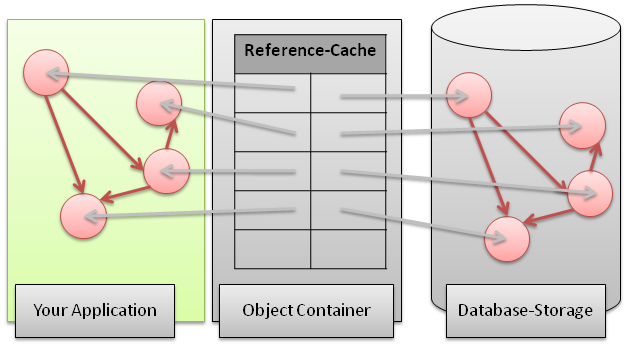
\includegraphics[width=\maxwidth]{images/ref-basics-indentity-concept-reference-cache.png}
\end{center}
\subsubsection*{Weak Reference}

By default db4o uses weak references in the reference cache. While your application has at least one references to an object, the reference cache has reference to it. But as soon as your application has no reference to the object anymore, it can be collected by the garbage collector. db4o will never prevent any object from being garbage collected. In the end persisted objects are garbage collected like any other objects.

To keep the cache clean, db4o does periodically remove all empty weak references. You can configure that clean-up interval. \hyperref[ref:configuration-common-weak-reference-collection-interval]{See "Weak Reference Collection Interval"} (p.~\pageref{ref:configuration-common-weak-reference-collection-interval})

You even can disable the weak reference. \hyperref[ref:configuration-common-disable-weak-references]{See "Disable Weak References"} (p.~\pageref{ref:configuration-common-disable-weak-references}). Then db4o holds regular references to your objects.This prevents the objects from being garbage collected. This means that you need to remove object from the reference cache manually. Or only use short living object containers. \hyperref[ref:advanced-topics-session-containers]{See "Session Containers"} (p.~\pageref{ref:advanced-topics-session-containers})

\subsubsection*{Manually Remove A Object From The Reference Cache}

You can manually remove a object from the reference cache. This only required when you have disabled the \hyperref[ref:configuration-common-disable-weak-references]{weak-references} (p.~\pageref{ref:configuration-common-disable-weak-references}).

\begin{lstlisting}
final Car theCar = container.query(Car.class).get(0);
container.ext().purge(theCar);
\end{lstlisting}

{\small\itshape IdentityConcepts.java: With purge you can remove objects from the reference cache\par}
\medskip

\section{Activation}
\label{ref:basics-activation}

Activation is a db4o mechanism which controls object instantiation. Why is it necessary? Let's look at an example of a stored tree structure. There's one root object, which has a bunch nodes. Each node has again a few subnodes and so on and so forth. What happens when you run a query and retrieve the root object? All the sub-objects will have to be created in the memory! If the tree is very large, this will fill up your memory.

\begin{center}
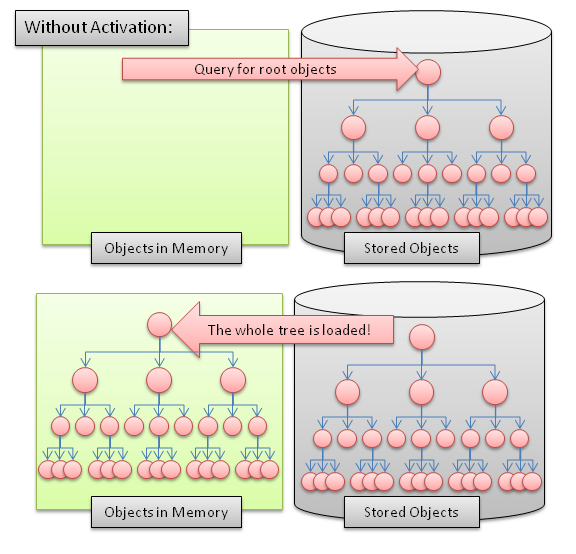
\includegraphics[width=\maxwidth]{images/ref-basics-activation-concept-without-activation.png}
\end{center}
Luckily db4o does not behave like this. When a query returns objects, they are loaded into memory (activated in db4o terms) only to a certain activation depth. In this case depth means "number of member references away from the original object". All the fields beyond the activation depth are set to null or to default values. So db4o does not load the whole object graph. Instead, db4o loads only the parts of the object graph you are interested in.

\begin{center}
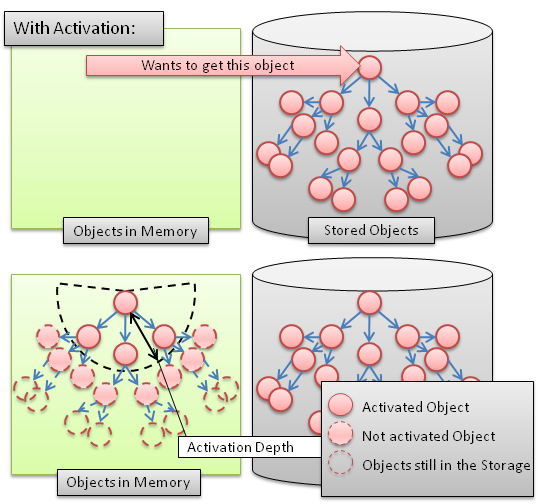
\includegraphics[width=\maxwidth]{images/ref-basics-activation-concept-with-activation.png}
\end{center}
Activation occurs in the following cases:

\begin{enumerate}
\item When you iterate over query results.
\item Object is activated explicitly with the object containers activate method.
\item Collections members are activated automatically, when the collection is activated, using at least depth 1 for lists and depth 2 for maps.
\end{enumerate}

For a concrete example of the activation process: \hyperref[ref:basics-activation-concept-hitting-activation-depth-wall]{See "Activation In Action"} (p.~\pageref{ref:basics-activation-concept-hitting-activation-depth-wall})

If you want to automate the activation process: \hyperref[ref:basics-activation-concept-transparent-activation-framework]{See "Transparent Activation"} (p.~\pageref{ref:basics-activation-concept-transparent-activation-framework})

\subsection{Activation In Action}
\label{ref:basics-activation-concept-hitting-activation-depth-wall}

Let's see db4o's activation in action. To see activation you need a deep object-graph. To keep this example simple we create a person class with a mother-field. This allows us to simply create a very deep object graph.

First the Person class:

\begin{lstlisting}
class Person {
    private Person mother;
    private String name;
    public Person(String name) {
        this.mother = mother;
        this.name = name;
    }

    public Person(Person mother, String name) {
        this.mother = mother;
        this.name = name;
    }

    public Person mother() {
        return mother;
    }

    public String getName() {
        return name;
    }
}
\end{lstlisting}

{\small\itshape Person.java: Person with a reference to the mother\par}
\medskip

After that store a deep hierarchy of persons, for example a hierarchy of seven people. Then query for it and traverse this object graph. When you hit the sixth person, that object won't be activated, because it's outside the activation depth. That object will have all fields set to null.

\begin{lstlisting}
final Person jodie = queryForJodie(container);
Person julia = jodie.mother().mother().mother().mother().mother();
// This will print null
// Because julia is not activated
// and therefore all fields are not set
System.out.println(julia.getName());
// This will throw a NullPointerException.
// Because julia is not activated
// and therefore all fields are not set
String joannaName = julia.mother().getName();
\end{lstlisting}

{\small\itshape ActivationDepthPitfall.java: Run into not activated objects\par}
\medskip

\subsubsection*{Use Explicit Activation}

When you traverse deep object graphs, you might run into not activated objects. Therefore you can activate objects explicitly.

\begin{lstlisting}
Person julia = jodie.mother().mother().mother().mother().mother();
container.activate(julia,5);

System.out.println(julia.getName());
String joannaName = julia.mother().getName();
System.out.println(joannaName);
\end{lstlisting}

{\small\itshape ActivationDepthPitfall.java: Fix with explicit activation\par}
\medskip

\subsubsection*{Configure Activation}

You can configure db4o to increase the activation depth. You can increase it \hyperref[ref:configuration-common-activation-depth]{globally} (p.~\pageref{ref:configuration-common-activation-depth}) or for \hyperref[ref:configuration-objectclass-minimum-activation-depth]{certain classes} (p.~\pageref{ref:configuration-objectclass-minimum-activation-depth}). Or you can \hyperref[ref:configuration-objectclass-cascade-on-activate]{cascade activate} (p.~\pageref{ref:configuration-objectclass-cascade-on-activate}) certain objects.

However remember that activation is there to improve the performance and save memory. If you set the activation depth to high it will hurt the performance.

\subsubsection*{Transparent Activation}

If you have a very complex model or don't want to deal with all the activation hassle then transparent activation is the best option. Transparent activation will manage the activation for you. \hyperref[ref:basics-activation-concept-transparent-activation-framework]{See "Transparent Activation Framework"} (p.~\pageref{ref:basics-activation-concept-transparent-activation-framework})

\subsubsection*{Deactivation}

It's also possible to deactivate an object. When you deactivate an object db4o sets all its fields back to their default value and considers it as deactivated. Deactivation is useful in rare cases where you want to return to the inactivated state for some reason.

\begin{lstlisting}
System.out.println(jodie.getName());
container.deactivate(jodie,5);
// Now all fields will be null or 0
// The same applies for all references objects up to a depth of 5
System.out.println(jodie.getName());
\end{lstlisting}

{\small\itshape ActivationDepthPitfall.java: Deactivate an object\par}
\medskip

\subsection{Transparent Activation}
\label{ref:basics-activation-concept-transparent-activation-framework}

Activation is a db4o-specific mechanism, which controls object instantiation in a query result. Activation works in several modes and is configurable on a database, object or field level. For more information see \hyperref[ref:basics-activation]{Activation} (p.~\pageref{ref:basics-activation}).

Using activation in a project with deep object hierarchies and many cross-references on different levels can make activation strategy complex and difficult to maintain. Transparent activation (TA) project was started to eliminate this problem and make activation automatic in the same time preserving the best performance and the lowest memory consumption.

With transparent activation enabled, objects are fetched on demand and only those that are used are being loaded.

Go to the \hyperref[ref:basics-transparent-persistence]{transparent activation / persistence chapter} (p.~\pageref{ref:basics-transparent-persistence}) to learn more about it.

\section{Update Concept}
\label{ref:basics-update-concept}

Updating objects in db4o is as easy as storing them. You just call then store-method again to update a object. How does a update work? There are two main questions. First, how does db4o recognize a object so that it knows whenever it should update a object or store it as a new object? And what's the scope of updates? All all objects updated? Or just the objects you explicitly store?

\subsection*{Object Recognition}

How does db4o know which object needs to be updated and which object has to be stored as new object? Well db4o uses the \hyperref[ref:basics-identity-concept]{object-identity} (p.~\pageref{ref:basics-identity-concept}) and looks up it if has loaded this object. If the object was loaded by db4o, it is an existing object and will be updated. Otherwise it has to be a new object and is stored as a new object.

\subsection*{Update Depth}

When you update of a object, db4o only stores the changes to a certain depth. This update depth avoids that db4o needs to go through the whole object graph and find out which objects have changed.

By default this update depth is one. This means when you update a object, only the changes on that object are stored. Changes on other objects are not included. When you want to store changes of multiple objects you need either to increase the \hyperref[ref:configuration-common-update-depth]{update-depth} (p.~\pageref{ref:configuration-common-update-depth}), store each object individually or use \hyperref[ref:basics-update-concept-transparent-persistence]{transparent persistence} (p.~\pageref{ref:basics-update-concept-transparent-persistence}).

Take a look at this concrete example to see how the update-depth affects you're operations. \hyperref[ref:basics-update-concept-update-depth-in-action]{See "Update Depth In Action"} (p.~\pageref{ref:basics-update-concept-update-depth-in-action})

Since collection are regular object in db4o the update depth also applies to collections. \hyperref[ref:basics-update-concept-updating-collections]{See "Updating Collections"} (p.~\pageref{ref:basics-update-concept-updating-collections})

If you want to automate the update process of object: \hyperref[ref:basics-update-concept-transparent-persistence]{See "Transparent Persistence"} (p.~\pageref{ref:basics-update-concept-transparent-persistence})

\subsection{Update Depth In Action}
\label{ref:basics-update-concept-update-depth-in-action}

Let's see db4o's update depth in action. We store a few cars with their pilots in the database. Then we update a car and its driver and store the car. The we reopen the database and check if everything was updated. To our surprise the car-name was updated, but the driver isn't. This is the direct result of db4o's update depth policy. It only updates object to a certain update-depth.

\begin{lstlisting}
ObjectContainer container = Db4oEmbedded.openFile(DATABASE_FILE);
try {
    Car car = queryForCar(container);
    car.setCarName("New Mercedes");
    car.getDriver().setName("New Driver Name");

    // With the default-update depth of one, only the changes
    // on the car-object are stored, but not the changes on
    // the person
    container.store(car);
} finally {
    container.close();
}
container = Db4oEmbedded.openFile(DATABASE_FILE);
try {
    Car car = queryForCar(container);
    System.out.println("Car-Name:"+car.getCarName());
    System.out.println("Driver-Name:"+car.getDriver().getName());
} finally {
    container.close();
}
\end{lstlisting}

{\small\itshape UpdateDepthPitfall.java: Update depth limits what is store when updating objects\par}
\medskip

\subsubsection*{Explicitly Store The Driver}

One solution to this issue is to store updated object explicitly, except value objects. So in our case we would store the car and the pilot. This works fine for simple models. However as the model gets more complex this is probably not a feasible solution.

\begin{lstlisting}
Car car = queryForCar(container);
car.setCarName("New Mercedes");
car.getDriver().setName("New Driver Name");

// Explicitly store the driver to ensure that those changes are also in the database
container.store(car);
container.store(car.getDriver());
\end{lstlisting}

{\small\itshape UpdateDepthPitfall.java: Explicitly store changes on the driver\par}
\medskip

There also a variation of this. You can use the store method of the extended container and explicitly state the update depth for the store operation.

\begin{lstlisting}
Car car = queryForCar(container);
car.setCarName("New Mercedes");
car.getDriver().setName("New Driver Name");

// Explicitly state the update depth
container.ext().store(car,2);
\end{lstlisting}

{\small\itshape UpdateDepthPitfall.java: Explicitly use the update depth\par}
\medskip

\subsubsection*{Configure Update Depth}

As alternative you can configure the update depth. You can increase it \hyperref[ref:configuration-common-update-depth]{globally} (p.~\pageref{ref:configuration-common-update-depth}) or for \hyperref[ref:configuration-objectclass-update-depth]{certain classes} (p.~\pageref{ref:configuration-objectclass-update-depth}). It's also possible to enable cascading updates for certain \hyperref[ref:configuration-objectclass-cascade-on-update]{classes} (p.~\pageref{ref:configuration-objectclass-cascade-on-update}) or \hyperref[ref:configuration-objectfield-configuration]{fields} (p.~\pageref{ref:configuration-objectfield-configuration}).

\subsubsection*{Transparent Persistence}

You can get rid of all the update depth troubles by using transparent persistence. In this mode db4o tracks all changes and stores them. \hyperref[ref:basics-update-concept-transparent-persistence]{See "Transparent Persistence"} (p.~\pageref{ref:basics-update-concept-transparent-persistence})

\subsection{Updating Collections}
\label{ref:basics-update-concept-updating-collections}

From the db4o perspective collections behave like ordinary objects. This means that the update-depth also applies to collections. When you change a collection and store the object which contains it, the changes are not stored by default.

\begin{lstlisting}
ObjectContainer container = Db4oEmbedded.openFile(DATABASE_FILE);
try {
    Person jodie = queryForJodie(container);
    jodie.add(new Person("Jamie"));
    // Remember that a collection is also a regular object
    // so with the default-update depth of one, only the changes
    // on the person-object are stored, but not the changes on
    // the friend-list.
    container.store(jodie);
} finally {
    container.close();
}
container = Db4oEmbedded.openFile(DATABASE_FILE);
try {
    Person jodie = queryForJodie(container);
    for (Person person : jodie.getFriends()) {
        // the added friend is gone, because the update-depth is to low
        System.out.println("Friend="+person.getName());
    }
} finally {
    container.close();
}
\end{lstlisting}

{\small\itshape UpdateDepthPitfall.java: Update doesn't work on collection\par}
\medskip

For collections the same rules and \hyperref[ref:basics-update-concept-update-depth-in-action]{settings work as for regular objects} (p.~\pageref{ref:basics-update-concept-update-depth-in-action}). For example when you increase the update depth to two, you can store the parent object and the changes of the collection are persisted as well.

\begin{lstlisting}
EmbeddedConfiguration config = Db4oEmbedded.newConfiguration();
config.common().updateDepth(2);
ObjectContainer container = Db4oEmbedded.openFile(config,DATABASE_FILE);
\end{lstlisting}

{\small\itshape UpdateDepthPitfall.java: A higher update depth fixes the issue\par}
\medskip

\subsection{Transparent Persistence}
\label{ref:basics-update-concept-transparent-persistence}

One of db4o's goals is to make the database transparent to the application logic. Wouldn't it be nice to initially register an object with a single store()-call and then let the database manage all future object modifications? Transparent Persistence does exactly that.It keeps track of changes and stores all modified objects automatically when committing.

This has several benefits:

\begin{itemize}
\item Clean an refactorable code. The code doesn't depend on the right activation-depth.
\item Performance-benefits. Only the objects which are needed are loaded into memory. And only modified objects are stored.
\item No changes can be lost due to miss configured update-depth.
\end{itemize}

To get started go to the \hyperref[ref:basics-transparent-persistence]{transparent activation/persistence topics} (p.~\pageref{ref:basics-transparent-persistence}).

\section{Transparent Activation/Persistence}
\label{ref:basics-transparent-persistence}

One of the challenges of db4o is to manage the \hyperref[ref:basics-activation]{activation of objects} (p.~\pageref{ref:basics-activation}). Also \hyperref[ref:basics-update-concept]{updating} (p.~\pageref{ref:basics-update-concept}) changed objects can be a challenge. The transparent activation/persistence framework solves these issues.

Transparent activation manages the activation of objects. It activates objects as soon as you access them. That means that you don't have to worry about the activation-depth or cascaded activation. As soon as you use transparent activation you don't need to configure any activation depth or cascading updates.

Transparent persistence builds on top of transparent activation and also manages updating objects. It monitors stored objects and memorizes changed objects. When you commit it automatically stores all updated objects. When you use transparent persistence you don't need any update depth nor cascade update configuration.

Transparent activation and persistence are very similar to implement. Therefore the same steps need to be taken to enable them.

To get started take a look at an example. \hyperref[ref:basics-transparentpersistence-ta-enhanced-example]{See "Transparent Persistence Enhanced Example"} (p.~\pageref{ref:basics-transparentpersistence-ta-enhanced-example})

For the learning the implementation details take a look at a manual implementation. \hyperref[ref:basics-transparentpersistence-implementation]{See "Implementation".} (p.~\pageref{ref:basics-transparentpersistence-implementation})

Collections need special attention in transparent activation / persistence. \hyperref[ref:basics-transparentpersistence-collections]{See "Collections".} (p.~\pageref{ref:basics-transparentpersistence-collections})

Also take a look at rollback strategies, which allows db4o to rollback in memory objects. \hyperref[ref:basics-transparentpersistence-automatic-deactivation]{See "Automatic Rollback"} (p.~\pageref{ref:basics-transparentpersistence-automatic-deactivation})

And finally take a look some well known pitfalls: \hyperref[ref:basics-transparentpersistence-transparent-activation-pitfalls]{See "Transparent Activation Pitfalls"} (p.~\pageref{ref:basics-transparentpersistence-transparent-activation-pitfalls})

\subsection{Manual Implementation}
\label{ref:basics-transparentpersistence-implementation}

This topic explains how transparent activation/persistence works and how you can implement the required interfaces manually. In practice you should use the \hyperref[ref:advanced-topics-enhancement-tools]{provided enhancer's} (p.~\pageref{ref:advanced-topics-enhancement-tools}) instead of implementing the interfaces yourself. \hyperref[ref:basics-transparentpersistence-ta-enhanced-example]{See "Transparent Persistence Enhanced Example"} (p.~\pageref{ref:basics-transparentpersistence-ta-enhanced-example})

\subsubsection{Adding the Configuration}
\label{ref:basics-transparentpersistence-implementation:adding}

We need to explicitly configure transparent activation/persistence.

\paragraph*{Transparent Activation}

This adds transparent activation, which automatically activates objects.

\begin{lstlisting}
final EmbeddedConfiguration configuration = Db4oEmbedded.newConfiguration();
configuration.common().add(new TransparentActivationSupport());
ObjectContainer container = Db4oEmbedded.openFile(configuration, DATABASE_FILE_NAME);
\end{lstlisting}

{\small\itshape TransparentPersistence.java: Add transparent activation\par}
\medskip

\paragraph*{Transparent Persistence}

This adds transparent persistence, which automatically activates objects and manages changes on objects. This includes implicitly the transparent activation support.

Optionally you can specify how \hyperref[ref:basics-transparentpersistence-automatic-deactivation]{rollbacks} (p.~\pageref{ref:basics-transparentpersistence-automatic-deactivation}) are handled.

\begin{lstlisting}
final EmbeddedConfiguration configuration = Db4oEmbedded.newConfiguration();
configuration.common().add(new TransparentPersistenceSupport(new DeactivatingRollbackStrategy()));
ObjectContainer container = Db4oEmbedded.openFile(configuration, DATABASE_FILE_NAME);
\end{lstlisting}

{\small\itshape TransparentPersistence.java: Add transparent persistence\par}
\medskip

\subsubsection{Implementing the Activatable Interface}
\label{ref:basics-transparentpersistence-implementation:implemen}

In order to support Transparent Activation, the objects which are stored in the database need to implement the Activatable-interface.

An object which implements the Activatable-interface is responsible for activating itself. For this purpose the class needs a field to keep its activator. This field is only used by the \hyperref[ref:basics-transparent-persistence]{transparent activation/persistence} (p.~\pageref{ref:basics-transparent-persistence}). Therefore it's marked as transient, to avoid that it is stored in the database.

\begin{lstlisting}
import com.db4o.activation.ActivationPurpose;
import com.db4o.activation.Activator;
import com.db4o.ta.Activatable;

public class Person implements Activatable{

    private transient Activator activator;
\end{lstlisting}

{\small\itshape Person.java: Implement the required activatable interface and add activator\par}
\medskip

The implementation of the two methods of the Activatable-interface is straight forward. The bind-method binds an activator to the object. It's called by the transparent activation framework. The activate-method needs to be called before any read or write operation on the object. Since these two methods are always the same, you can move the implementation to a common super class or to a static utility class.

\begin{lstlisting}
public void bind(Activator activator) {
    if (this.activator == activator) {
        return;
    }
    if (activator != null && null != this.activator) {
        throw new IllegalStateException("Object can only be bound to one activator");
    }
    this.activator = activator;
}

public void activate(ActivationPurpose activationPurpose) {
    if(null!=activator){
        activator.activate(activationPurpose);
    }
}
\end{lstlisting}

{\small\itshape Person.java: Implement the activatable interface methods\par}
\medskip

Now to the most important part. Every time a field of the class is accessed you need to call the activate-method with the purpose. This needs to be done in every getter/setter and method. Probably the best way is to use only getter/setter even within the class to access fields. And the getter/setter ensures that the activate-method is called.

\begin{lstlisting}
public void setName(String name) {
    activate(ActivationPurpose.WRITE);
    this.name = name;
}

public String getName()  {
    activate(ActivationPurpose.READ);
    return name;
}

public String toString()  {
    // use the getter/setter withing the class,
    // to ensure the activate-method is called
    return getName();
}
\end{lstlisting}

{\small\itshape Person.java: Call the activate method on every field access\par}
\medskip

Implementing the Activatable-interface manually for every class is repetitive and error prone. That's why this process can be automated.\hyperref[ref:basics-transparentpersistence-ta-enhanced-example]{See "Transparent Persistence Enhanced Example"} (p.~\pageref{ref:basics-transparentpersistence-ta-enhanced-example})

After transparent activation/persistence is enabled you can navigate into object-graph as deeply as you want. The transparent activation will load the objects from the database as you need them. When you've enabled transparent persistence updates are also done transparently.

\begin{lstlisting}
{
    ObjectContainer container = openDatabaseWithTA();
    Person person = Person.personWithHistory();
    container.store(person);
    container.close();
}
{
    ObjectContainer container = openDatabaseWithTA();
    Person person = queryByName(container,"Joanna the 10");
    Person beginOfDynasty = person.getMother();

    // With transparent activation enabled, you can navigate deeply
    // nested object graphs. db4o will ensure that the objects
    // are loaded from the database.
    while(null!=beginOfDynasty.getMother()){
        beginOfDynasty = beginOfDynasty.getMother();
    }
    System.out.println(beginOfDynasty.getName());
    
    container.close();
}
\end{lstlisting}

{\small\itshape TransparentActivationExamples.java: Transparent activation in action\par}
\medskip

\subsubsection{Behavior in Mixed Mode}
\label{ref:basics-transparentpersistence-implementation:behavior}

In some environments there are both, objects which implement the Activatable-interface on other which don't. What's the behavior in this scenario? Then the behavior is this:

\begin{itemize}
\item Objects which implement the Activatable-interface are activated when they are used the first time.
\item Objects which do not implement the Activatable-interface are always fully loaded.
\end{itemize}

That behavior ensures that you never run into not activated objects in the transparent activation / persistence mode.

However objects which do not implement the Activatable-interface are not updated with transparent persistence. You have to do that yourself or enhance those classes as well.

\subsection{Enhancement Example}
\label{ref:basics-transparentpersistence-ta-enhanced-example}

You can inject transparent persistence awareness in your persisted classes without modifying their original code. This is done by enhancing the class-files at build time.

\subsubsection{Required Depedencies}
\label{ref:basics-transparentpersistence-ta-enhanced-example:dependencies}

For transparent activation/persistence you need following dependencies at compile time. (see also the \hyperref[ref:dependency-overview]{dependency overview} (p.~\pageref{ref:dependency-overview}))

\begin{itemize}
\item db4o-8.1-bloat.jar
\item db4o-8.1-instrumentation.jar
\item db4o-8.1-taj.jar
\item db4o-8.1-tools.jar
\end{itemize}

\subsubsection{Enhance Persistent Classes}
\label{ref:basics-transparentpersistence-ta-enhanced-example:enhance}

The first step is to enhance the persisted classes. One possibility is to introduce an Annotation to mark your persisted classes.

By the way, their are alternative way to select the enhanced classes. See  \hyperref[ref:advanced-topics-enhancement-tools-enhancement-for-java-build-time-enhancement]{here} (p.~\pageref{ref:advanced-topics-enhancement-tools-enhancement-for-java-build-time-enhancement}).

\begin{lstlisting}
@Retention(RetentionPolicy.RUNTIME)
@Documented
@Target(ElementType.TYPE)
public @interface TransparentPersisted {
}
\end{lstlisting}

{\small\itshape TransparentPersisted.java: Annotation to mark persisted classes\par}
\medskip

This Annotation is then used to mark all persisted classes.

\begin{lstlisting}
@TransparentPersisted
public class Person {
\end{lstlisting}

{\small\itshape Person.java: Mark your domain model with the annotations\par}
\medskip

The next step is to create a class filter which reports all classes which should be enhanced. There filter checks for the presence of the annotation.

\begin{lstlisting}
public final class AnnotationFilter implements ClassFilter {

    public boolean accept(Class<?> aClass) {
        if(null==aClass || aClass.equals(Object.class)){
            return false;
        }
        return hasAnnotation(aClass)
                || accept(aClass.getSuperclass());
    }

    private boolean hasAnnotation(Class<?> aClass) {
        // We compare by name, to be class-loader independent
        Annotation[] annotations = aClass.getAnnotations();
        for (Annotation annotation : annotations) {
            if(annotation.annotationType().getName()
                    .equals(TransparentPersisted.class.getName())){
                return true;
            }
        }
        return false;
    }

}
\end{lstlisting}

{\small\itshape AnnotationFilter.java: Build a filter\par}
\medskip

\subsubsection*{Enhancing Classes Using Ant}

This enhancement step injects the required bytecode into the domain classes to support transparent activation/persistence.

\begin{lstlisting}
<target name="enhance">
    <!-- Change these according to your project -->
    <property name="target" value="./target/classes/"/>
    <property name="libraries" value="./lib/"/>

    <path id="project.classpath">
        <pathelement path="${target}"/>
        <fileset dir="${libraries}">
            <include name="*.jar"/>
        </fileset>
    </path>

    <!-- We enhance with an additional Ant-run step. You can put this also in an extra file -->
    <typedef resource="instrumentation-def.properties"
             classpathref="project.classpath"
             loaderRef="instrumentation.loader"/>

    <!-- We filter by our annotation -->
    <typedef name="annotation-filter"
             classname="com.db4odoc.tp.enhancement.AnnotationFilter"
             classpathref="project.classpath"
             loaderRef="instrumentation.loader"/>

    <db4o-instrument classTargetDir="${target}"
                  verbose="true">
        <classpath refid="project.classpath"/>
        <sources dir="${target}">
            <include name="**/*.class"/>
        </sources>

        <transparent-activation-step>
            <annotation-filter/>
        </transparent-activation-step>
    </db4o-instrument>
</target>
\end{lstlisting}

{\small\itshape enhance-with-annotation.xml: Ant target for enhancing your classes after building them\par}
\medskip

\subsubsection*{Configure Eclipse to Run Ant Target}

You can configure Eclipse to run the Ant build with each compile step. Right click on your project and choose 'Properties'. Then switch to 'Builders' and add a new one. Choose the 'Ant Builder'. On the new window choose the build-file which contains the example-code. Switch to the 'Targets'-Tab. There choose the enhance-target for the 'Auto-Build'. Now the enhancer-task will be run by Eclipse automatically. The example project above is configured this way.

\subsubsection*{Enhancing Classes Using Maven}

It's also possible to enhance with Maven by using the \href{http://maven.apache.org/plugins/maven-antrun-plugin/}{Ant plugin}.

\begin{lstlisting}
<plugin>
    <artifactId>maven-antrun-plugin</artifactId>
    <version>1.6</version>
    <dependencies>
        <!-- We need the db4o tooling for enhancing stuff -->
        <dependency>
            <groupId>com.db4o</groupId>
            <artifactId>db4o-tools-java5</artifactId>
            <version>8.1-SNAPSHOT</version>
        </dependency>
    </dependencies>
    <executions>
        <execution>
            <phase>compile</phase>
            <configuration>
                <target>
                    <!-- We enhance with an additional Ant-run step. You can put this also in an extra file -->
                    <typedef resource="instrumentation-def.properties"
                             classpathref="maven.compile.classpath"/>

                    <!-- We filter by our annotation -->
                    <typedef name="annotation-filter"
                             classname="com.db4odoc.tp.enhancement.AnnotationFilter"
                             classpathref="maven.compile.classpath"/>

                    <db4o-instrument classTargetDir="target/classes"
                              verbose="true">
                        <classpath refid="maven.compile.classpath"/>
                        <sources dir="target/classes">
                            <include name="**/*.class"/>
                        </sources>

                        <transparent-activation-step>
                            <annotation-filter/>
                        </transparent-activation-step>
                    </db4o-instrument>
                </target>
            </configuration>
            <goals>
                <goal>run</goal>
            </goals>
        </execution>
    </executions>
</plugin>
\end{lstlisting}

{\small\itshape pom.xml: Enhance persisted classes during the build\par}
\medskip

\subsubsection{Check Enhancement}
\label{ref:basics-transparentpersistence-ta-enhanced-example:check}

You can check if the enhancement worked correctly by checking for the activation interface. Such a check should be part of your test-suite to ensure that everything works correctly.

\begin{lstlisting}
if (!Activatable.class.isAssignableFrom(Person.class)) {
    throw new AssertionError("Expect that the " + Person.class + " implements " + Activatable.class);
}
\end{lstlisting}

{\small\itshape TransparentPersistence.java: Check for enhancement\par}
\medskip

\subsubsection{Using Transparent Activation / Persistence}
\label{ref:basics-transparentpersistence-ta-enhanced-example:usingtp}

Configure the transparent activation in order to use it.

\begin{lstlisting}
final EmbeddedConfiguration configuration = Db4oEmbedded.newConfiguration();
configuration.common().add(new TransparentActivationSupport());
ObjectContainer container = Db4oEmbedded.openFile(configuration, DATABASE_FILE_NAME);
\end{lstlisting}

{\small\itshape TransparentPersistence.java: Add transparent activation\par}
\medskip

After that transparent activation is working properly you can transverse along the object graph and don't have to worry about not activated objects:

\begin{lstlisting}
Person person = queryByName(container, "Joanna the 10");
Person beginOfDynasty = person.getMother();

// With transparent activation enabled, you can navigate deeply
// nested object graphs. db4o will ensure that the objects
// are loaded from the database.
while (null != beginOfDynasty.getMother()) {
    beginOfDynasty = beginOfDynasty.getMother();
}
System.out.println(beginOfDynasty.getName());
\end{lstlisting}

{\small\itshape TransparentPersistence.java: Activation just works\par}
\medskip

\subsubsection*{Using Transparent Persistence}

Transparent persistence not only manages the activation, but also manages updating the objects. Configure transparent persistence in order to use it:

\begin{lstlisting}
final EmbeddedConfiguration configuration = Db4oEmbedded.newConfiguration();
configuration.common().add(new TransparentPersistenceSupport(new DeactivatingRollbackStrategy()));
ObjectContainer container = Db4oEmbedded.openFile(configuration, DATABASE_FILE_NAME);
\end{lstlisting}

{\small\itshape TransparentPersistence.java: Add transparent persistence\par}
\medskip

After that updated objects are automatically stored every time you commit.

\begin{lstlisting}
Person person = queryByName(container, "Joanna the 10");
Person mother = person.getMother();
mother.setName("New Name");
// Just commit the transaction. All modified objects are stored
container.commit();
\end{lstlisting}

{\small\itshape TransparentPersistence.java: Just update and commit. Transparent persistence manages all updates\par}
\medskip

\subsection{Collections}
\label{ref:basics-transparentpersistence-collections}

In order to support transparent persistence properly, a class has to implement the Activatable-interface. For your domain classes this is easy to archive. But what about Java-collections? Wouldn't it be nice when collections also work together the transparent activation framework?

db4o brings special, transparent persistence aware collections with it. This collections load the content only when the collections is actually used.

These collections are currently implemented:

\begin{itemize}
\item ActivatableArrayList\textless{}T\textgreater{}: An activatable version of the ArrayList\textless{}T\textgreater{}
\item ActivatableHashMap\textless{}T\textgreater{}: An activatable version of the HashMap\textless{}T\textgreater{}
\item ActivatableHashSet\textless{}T\textgreater{}: An activatable version of the HashSet\textless{}T\textgreater{}
\item ActivatableHashtable\textless{}T\textgreater{}: An activatable version of the HashHashtable\textless{}T\textgreater{}
\item ActivatableLinkedList\textless{}T\textgreater{}: An activatable version of the LinkedList\textless{}T\textgreater{}
\item ActivatableStack\textless{}T\textgreater{}: An activatable version of the Stack\textless{}T\textgreater{}
\item ActivatableTreeSet\textless{}T\textgreater{}: An activatable version of the TreeSet\textless{}T\textgreater{}
\end{itemize}

It's recommended to use the collection-interfaces wherever possible instead of the concrete classes. This avoids unnecessary direct dependencies on the implementations and makes it easy to exchange the implementations.

The enhancement tools can automatically replace the Java-collections with the db4o-equivalent. However there are few rules and limitations. \hyperref[ref:basics-transparentpersistence-collections-enhance-collections]{See "Enhance Collections"} (p.~\pageref{ref:basics-transparentpersistence-collections-enhance-collections})

You can use the db4o-collection directly in your code. For example in the case you implement the transparent activation support manually. Take a looks these tips: \hyperref[ref:basics-transparentpersistence-collections-use-ta-collections]{See "Using Transparent Activatable Collections Directly"} (p.~\pageref{ref:basics-transparentpersistence-collections-use-ta-collections})

\subsubsection{Using TA Collections Directly}
\label{ref:basics-transparentpersistence-collections-use-ta-collections}

You can use the transparent activation aware collections directly in your code. Their behavior is the same as the Java-collections. Here are a few tips:

\begin{itemize}
\item Prefer the collection-interfaces over the concrete classes in your field-, parameter- and return-type declarations. For example declare a field as a List\textless{}T\textgreater{} instead of an ArrayList\textless{}T\textgreater{}
\item Maybe it is useful to create a collection factory in your code. Then you have only one place in your code which decides which implementation is used. That makes it easy to replace the implementations.
\end{itemize}

An example:

\begin{lstlisting}
public class Team  extends AbstractActivatable{ 

    private List<Pilot> pilots = new ActivatableArrayList<Pilot>();

    public boolean add(Pilot pilot) {
        activate(ActivationPurpose.WRITE);
        return pilots.add(pilot);
    }

    public Collection<Pilot> getPilots(){
        activate(ActivationPurpose.READ);
        return pilots;
    }
}
\end{lstlisting}

{\small\itshape Team.java: Using the activation aware collections\par}
\medskip

Currently these collections are available:

\begin{itemize}
\item ActivatableArrayList\textless{}T\textgreater{}: An activatable version of the ArrayList\textless{}T\textgreater{}
\item ActivatableHashMap\textless{}T\textgreater{}: An activatable version of the HashMap\textless{}T\textgreater{}
\item ActivatableHashSet\textless{}T\textgreater{}: An activatable version of the HashSet\textless{}T\textgreater{}
\item ActivatableHashtable\textless{}T\textgreater{}: An activatable version of the HashHashtable\textless{}T\textgreater{}
\item ActivatableLinkedList\textless{}T\textgreater{}: An activatable version of the LinkedList\textless{}T\textgreater{}
\item ActivatableStack\textless{}T\textgreater{}: An activatable version of the Stack\textless{}T\textgreater{}
\item ActivatableTreeSet\textless{}T\textgreater{}: An activatable version of the TreeSet\textless{}T\textgreater{}
\end{itemize}

\subsubsection{Enhance Collections}
\label{ref:basics-transparentpersistence-collections-enhance-collections}

You can use the normal Java-collections in your code and then replace the implementations with the enhancement-tools. \hyperref[ref:basics-transparentpersistence-ta-enhanced-example]{See "Transparent Persistence Enhanced Example"} (p.~\pageref{ref:basics-transparentpersistence-ta-enhanced-example})

The enhancement tools will search for instantiations of collections and replace it with an appropriate transparent activation aware collection.

The transparent persistence aware collections are always subclasses of the Java-collections. Therefore all methods are available. Furthermore potential cast or instanceof checks also work without any problem.

\subsection{Rollback Strategy}
\label{ref:basics-transparentpersistence-automatic-deactivation}

When you \hyperref[ref:basics-acid-and-transactions]{rollback a transaction} (p.~\pageref{ref:basics-acid-and-transactions}) only the state of database affected. The state of the objects in memory isn't touched by the rollback method. Wouldn't it be nice when the objects in memory are also rolled back on a transaction rollback? This can be done by providing a rollback strategy for the transparent persistence. For that you need to pass a RollbackStrategy-implementation to the transparent persistence support. The rollback method will be automatically called once per modified object after a rollback. On the rollback method you can deactivate the modified object. This ensures that the object state is cleared and read again from the database. This is a simple but effective strategy and therefore is implemented in the DeactivatingRollbackStrategy.

\begin{lstlisting}
EmbeddedConfiguration configuration = Db4oEmbedded.newConfiguration();
configuration.common()
        .add(new TransparentPersistenceSupport(new DeactivatingRollbackStrategy()));
\end{lstlisting}

{\small\itshape RollbackExample.java: Configure rollback strategy\par}
\medskip

After adding the rollback strategy objects are rolled back aswell.

\begin{lstlisting}
Pilot pilot = container.query(Pilot.class).get(0);
pilot.setName("NewName");
// Rollback
container.rollback();
// Now the pilot has the old name again
System.out.println(pilot.getName());
\end{lstlisting}

{\small\itshape RollbackExample.java: Rollback with rollback strategy\par}
\medskip

Note that rollback strategies only work for activatable objects.

\subsection{Transparent Activation Pitfalls}
\label{ref:basics-transparentpersistence-transparent-activation-pitfalls}

\hyperref[ref:basics-activation-concept-transparent-activation-framework]{Transparent Persistence} (p.~\pageref{ref:basics-activation-concept-transparent-activation-framework}) is a powerful feature that can make your development much faster, easier and more error-proof. However it can lead to trouble if used in a wrong way. The aim of this chapter is to point you out to typical pitfalls, which lead to unexpected and undesired results.

\subsubsection*{Not Activate Call Before Field Access}

Before accessing any field you need to call the activate-method. This is true for all getter/setter and also for other methods like the toString-method. The best strategy is to call the activate-method in the getter/setter and then access the field through those even in the class itself.

Or use the \hyperref[ref:advanced-topics-enhancement-tools]{enhancement-tools} (p.~\pageref{ref:advanced-topics-enhancement-tools}) to avoid this issue complete.

\subsubsection*{Migrating Between Databases}

\paragraph*{Problem}

Transparent Activation is implemented through the Activatable-interface, which binds an object to the current object container. When an object is stored in more than one object container, this logic won't work, as only one binding is allowed per object.

\paragraph*{Solution}

To allow correct behavior of the object between databases, the object should be unbound before being stored to the another database.Just set the activator to null.

\subsubsection*{Instrumentation Limitations}

\paragraph*{Problem}

For Java built time enhancement the classes to instrument should be on the classpath.

\paragraph*{Solution}

Make sure that all classes to be instrumented are available through the classpath

\subsubsection*{Debugging Instrumented Classes}

Debugging instrumented classes may not work 100\% correct.

You should be able to debug normally anywhere around instrumented bytecode. If you still think that the problem occurs in the instrumented area, please report a bug through the \href{https://github.com/blakemcbride/db4o}{db4o repository}.

\section{Delete Behavior}
\label{ref:basics-delete-behavior}

Deleting an object is as simple as storing an object. You simply call the delete-method on the container to delete it. By default only the object you pass to the delete method is deleted. All referenced objects are not deleted.

\begin{lstlisting}
Car car = findCar(container);
container.delete(car);
// We've deleted the only care there is
assertEquals(0,allCars(container).size());
// The pilots are still there
assertEquals(1,allPilots(container).size());
\end{lstlisting}

{\small\itshape DeletionExamples.java: Deleting object is as simple as storing\par}
\medskip

\subsection*{Reference To Deleted Objects}

What happens when you delete a object which is still referenced by other objects? Well in such cases that reference is set to null.

\begin{lstlisting}
Pilot pilot = findPilot(container);
container.delete(pilot);
\end{lstlisting}

{\small\itshape DeletionExamples.java: Delete the pilot\par}
\medskip

\begin{lstlisting}
// Now the car's reference to the car is set to null
Car car = findCar(container);
assertEquals(null,car.getPilot());
\end{lstlisting}

{\small\itshape DeletionExamples.java: Reference is null after deleting\par}
\medskip

Often you want to ensure that a object isn't referenced anymore, before you can delete it. However such referential integrity isn't supported at the moment. You need to implement your integrity checks manually, for example with \hyperref[ref:advanced-topics-callbacks]{callbacks} (p.~\pageref{ref:advanced-topics-callbacks}).

\subsection*{Cascading Deletion And Collections.}

Additionally you can configure cascading behavior for deletion. \hyperref[ref:basics-delete-behavior-cascading-deletion]{See "Cascading Deletion"} (p.~\pageref{ref:basics-delete-behavior-cascading-deletion})

Also collections are treated like regular objects and need to be deleted explicitly. \hyperref[ref:basics-delete-behavior-collections]{See "Collections And Arrays"} (p.~\pageref{ref:basics-delete-behavior-collections})

\subsection{Cascading Deletion}
\label{ref:basics-delete-behavior-cascading-deletion}

By default db4o only deletes objects which are passed to the delete-method and doesn't delete referenced objects. You can easily change that. Configure the cascading deletion behavior in the configuration for \hyperref[ref:configuration-objectclass-cascade-on-delete]{certain classes} (p.~\pageref{ref:configuration-objectclass-cascade-on-delete}) or \hyperref[ref:configuration-objectfield-configuration]{certain fields} (p.~\pageref{ref:configuration-objectfield-configuration}).

For example we mark that the object in the 'pilot'-field is also deleted:

\begin{lstlisting}
EmbeddedConfiguration config = Db4oEmbedded.newConfiguration();
config.common().objectClass(Car.class).objectField("pilot").cascadeOnDelete(true);
ObjectContainer container = Db4oEmbedded.openFile(config,DATABASE_FILE);
\end{lstlisting}

{\small\itshape DeletionExamples.java: Mark field for cascading deletion\par}
\medskip

When we now delete the car, the pilot of that car is also deleted.

\begin{lstlisting}
Car car = findCar(container);
container.delete(car);
// Now the pilot is also gone
assertEquals(0,allPilots(container).size());
\end{lstlisting}

{\small\itshape DeletionExamples.java: Cascade deletion\par}
\medskip

\subsection{Collections and Arrays}
\label{ref:basics-delete-behavior-collections}

Collections and arrays don't have a special behavior in db4o. When you delete a collection, the collection-members are not deleted. The collection and objects are two independent objects for db4o.

\subsubsection*{Removing From A Collection}

To remove object from a collection you can simple use the regular collection-operations and then store that collection.

\begin{lstlisting}
PilotGroup group = findGroup(container);
final Pilot pilot = group.getPilots().get(0);
group.getPilots().remove(pilot);
container.store(group.getPilots());

assertEquals(3,allPilots(container).size());
assertEquals(2,group.getPilots().size());
\end{lstlisting}

{\small\itshape DeletionExamples.java: Removing from a collection doesn't delete the collection-members\par}
\medskip

\subsubsection*{Remove And Delete Collection Members}

If you want to delete a collection-member, remove it and then delete it.

\begin{lstlisting}
PilotGroup group = findGroup(container);
final Pilot pilot = group.getPilots().get(0);
group.getPilots().remove(pilot);
container.store(group.getPilots());
container.delete(pilot);

assertEquals(2,allPilots(container).size());
assertEquals(2,group.getPilots().size());
\end{lstlisting}

{\small\itshape DeletionExamples.java: Remove and delete\par}
\medskip

\section{Indexing}
\label{ref:basics-indexing}

db4o supports indexes like most databases do. Indexes are data structures which allow efficient lookup of data. When you enable an index, db4o will add an entry to index for each object. This makes the insert and update operation a little slower. However it makes queries a lot faster. A query which uses an index is a order of magnitude faster that a query which cannot use a index.

You can create a index by enabling it on a field. \hyperref[ref:configuration-objectfield-configuration]{See "Adding a Field Index"} (p.~\pageref{ref:configuration-objectfield-configuration})

\begin{lstlisting}
@Indexed
private String zipCode;
\end{lstlisting}

{\small\itshape City.java: Index a field\par}
\medskip

As an alternative you can configure a field index externally.

\begin{lstlisting}
EmbeddedConfiguration configuration = Db4oEmbedded.newConfiguration();
configuration.common().objectClass(Person.class).objectField("name").indexed(true);
\end{lstlisting}

{\small\itshape ObjectFieldConfigurations.java: Index a certain field\par}
\medskip

\subsection*{When And Where Do I Need An Index}

When do you need an index? As a rule of thumb: Add an index all fields which are used in queries. \hyperref[ref:basics-indexing-when-and-where]{See "When And Where"} (p.~\pageref{ref:basics-indexing-when-and-where})

There are different factors which need to be fulfilled to profit from an index.

\begin{itemize}
\item Read operations dominate the database operations: When you application only writes objects but rarely query for objects, there's no benefit of faster queries. However in most system reading is the dominate operation and should be fast.
\item You're using the field / class in a query: If no query touches the field or class you're have a index on, you have not benefit from the index. The index improves only the query performance, but slows down store and update-operations.
\item You actually need a substantial amount of data. The performance gains of an index are negligible for small data sets. When you test indexes use 10'000 and more objects.
\end{itemize}

\subsection{When And Where}
\label{ref:basics-indexing-when-and-where}

When do you need an index? And on which fields do I need an index? An index has a costs and benefits. \hyperref[ref:basics-indexing-costs-and-benefits]{See "Costs And Benefits"} (p.~\pageref{ref:basics-indexing-costs-and-benefits}). Therefore you should only add one when you actually benefit from it.

\subsubsection*{When To Add Queries}

Indexes speed up queries but slow down store and delete operations. You only need to add indexes when queries are too slow. There's no real benefit to add a index when your queries are already fast enough.

Also add index only on fields which are used in queries. Indexes on fields which are never used in a query have no benefit.

\subsubsection*{Where To Add Queries}

How do I find the queries which can benefit from indexes? How do I find queries which couldn't utilize indexes? You can use the \hyperref[ref:configuration-common-diagnostics]{diagnostic-API} (p.~\pageref{ref:configuration-common-diagnostics}) find out. Filter for the LoadedFromClassIndex-message. Every time this message arrives the query didn't use a field index. You can add a break-point to the message-output and find out which query is the source and then add the index.

\begin{lstlisting}
configuration.common().diagnostic().addListener(new DiagnosticListener() {
    @Override
    public void onDiagnostic(Diagnostic diagnostic) {
        if(diagnostic instanceof LoadedFromClassIndex)
        {
            System.out.println("This query couldn't use field indexes "+
                ((LoadedFromClassIndex)diagnostic).reason());
            System.out.println(diagnostic);
        }
    }
});
\end{lstlisting}

{\small\itshape WhereToIndexExample.java: Find queries which cannot use index\par}
\medskip

\subsection{Costs And Benefits}
\label{ref:basics-indexing-costs-and-benefits}

Maintaining an index is additional work and therefore it has its costs. Each time you store a objects which has an index on it, db4o needs to look up the a appropriate place in the index and store a entry there. This costs is paid for each store, update or delete operation. Therefore there's a tradeoff when adding indexes.

The costs are mostly the time consumed to maintain the index. Additionally there's some additional space consumed to store the index. The benefits is that queries which run a order of magnitude faster when using an index.

In practice you should measure and benchmark your solution and check if a index is a benefit to your application. Ensure that you have enough test data. The influence of indexes shows better with a lot of objects. (10'000 and more objects). However since most applications do a lot more read operations than store and update operations adding a index brings a huge benefit.

\subsection{Types And Limitations}
\label{ref:basics-indexing-types-and-limitations}

There are limitations to the db4o indexing. Not all types can be indexed.

\subsubsection*{Types Which Can Be Indexed}

Basically all primitive types like int, long, double etc can be indexed. Indexes on primitive types work extremely well.

Additionally you can index strings, which are handled by db4o like primitives. Strings can be arbitrary long, so a index on string is usually slower than a index on a primitive value. But it's still fast for straight lookups. Note also that a string index can only be used for equality comparison. Comparisons like contains, start with etc don't use the index.

The Date  can also be indexed without any issues.

You also can index any object reference except arrays and strings, which are handled like primitives. This means you can index a field which holds a reference to a object and then look up for objects which have a certain reference.

You can also index BigDecimal and BigNumber objects. Those indexes act like indexes on regular primitive types like int or long. Note that you need to add \hyperref[ref:advanced-topics-type-handling-bigmath]{BigMath-support} (p.~\pageref{ref:advanced-topics-type-handling-bigmath}).

\subsubsection*{Types Which Cannot Be Indexed}

Arrays and collections cannot be indexed. The current db4o index implementation cannot deal with those types. This also means that you cannot do fast look-ups on arrays or collections.

\subsubsection*{Limitations}

Currently the index on strings cannot be used for advanced comparisons like contains, starts with etc.

\subsection{Check For Existing Indexes}
\label{ref:basics-indexing-check-for-index}

Sometime you may want to know if a index exists on a certain field. You can use the \hyperref[ref:advanced-topics-db4o-meta-information]{db4o-meta information} (p.~\pageref{ref:advanced-topics-db4o-meta-information}) to find out if a field is indexed.

\begin{lstlisting}
StoredClass metaInfo = container.ext().storedClass(IndexedClass.class);
// list a fields and check if they have a index
for (StoredField field : metaInfo.getStoredFields()) {
    if(field.hasIndex()){
        System.out.println("The field '"+field.getName()+"' is indexed");
    } else{
        System.out.println("The field '"+field.getName()+"' isn't indexed");
    }
}
\end{lstlisting}

{\small\itshape CheckForAndIndex.java: Check for a index\par}
\medskip

\subsection{Traversing the Index Values}
\label{ref:basics-indexing-traverse-index}

The db4o query processor uses the index to speed up queries. So you just use the query APIs to benefit from indexes. For special cases you might want to traverse the indexed values yourself. You can do this by accessing the index via the \hyperref[ref:advanced-topics-db4o-meta-information]{db4o meta data} (p.~\pageref{ref:advanced-topics-db4o-meta-information}). There you can get the meta-info for a field and then traverse its index. Note that the traverse-method will throw an exception if there is no index available.

\begin{lstlisting}
final StoredField storedField = container.ext()
        .storedClass(Item.class).storedField("data", int.class);
storedField.traverseValues(new Visitor4<Integer>() {
    @Override
    public void visit(Integer fieldValue) {
        System.out.println("Value "+fieldValue);
    }
});
\end{lstlisting}

{\small\itshape TraverseIndexExample.java: Traverse index\par}
\medskip


% Converted from reference/DB4OFlare (MadCap Flare, Java target)

\chapter{Advanced Features}
\label{ref:advanced-topics}

This topic is about advanced features of db4o.

If you want to have multiple unit of work or multiple transaction in embedded mode you can take a look at session containers. \hyperref[ref:advanced-topics-session-containers]{See "Session Containers"} (p.~\pageref{ref:advanced-topics-session-containers})

db4o support unique constrains on fields. \hyperref[ref:advanced-topics-unique-constraints]{See "Unique Constraints"} (p.~\pageref{ref:advanced-topics-unique-constraints})

You can also do backups of your database at runtime. \hyperref[ref:advanced-topics-backup]{See "Backup"} (p.~\pageref{ref:advanced-topics-backup})

Implementing the interfaces for transparent activation/persistence is tedious. The enhancement tools can do that job for you. And can also optimize native queries at build time. \hyperref[ref:advanced-topics-enhancement-tools]{See "Enhancement Tools"} (p.~\pageref{ref:advanced-topics-enhancement-tools})

The database file can fragment over time. In order to reclaim defragmentet space in the database you need to run the defragmentation. \hyperref[ref:advanced-topics-defragment]{See "Defragment"} (p.~\pageref{ref:advanced-topics-defragment})

Callbacks allow you to perform additional logic for different database operations. \hyperref[ref:advanced-topics-callbacks]{See "Callbacks"} (p.~\pageref{ref:advanced-topics-callbacks})

As some point in time you will change your data model. Then you probably need to also refactor you're stored data in the database. \hyperref[ref:advanced-topics-refactoring-and-schema-evolution]{See "Refactoring and Schema Evolution"} (p.~\pageref{ref:advanced-topics-refactoring-and-schema-evolution})

You can access the internal ids or generate UUIDs for objects. \hyperref[ref:advanced-topics-ids-and-uuids]{See "IDs and UUIDs"} (p.~\pageref{ref:advanced-topics-ids-and-uuids})

It's also possible to access the meta information of all stored types in the database. \hyperref[ref:advanced-topics-db4o-meta-information]{See "db4o Meta-Information"} (p.~\pageref{ref:advanced-topics-db4o-meta-information}). And you can access system information about the database.

db4o tried hard to make persisting objects as easy as possible. However storing a object efficient and correctly is quite tricky. Read about db4o's type handling for more information. \hyperref[ref:advanced-topics-type-handling]{See "Type Handling"} (p.~\pageref{ref:advanced-topics-type-handling}) Furthermore db4o uses an abstraction layer to encapsulate Java-reflection. This allows you do change how reflection behaves on your objects. \hyperref[ref:advanced-topics-db4o-reflection-api]{See "db4o Reflection API"} (p.~\pageref{ref:advanced-topics-db4o-reflection-api})

Unfortunately failure happen. db4o communicates failures with exceptions. \hyperref[ref:advanced-topics-exceptions]{See "Exception-Handling"} (p.~\pageref{ref:advanced-topics-exceptions})

\section{Session Containers}
\label{ref:advanced-topics-session-containers}

In an application there are often multiple operations running at the same time. A typical example is a web application which processes multiple requests at the same time. These operations should be isolated from each other. This means that for the database we want to have multiple transactions at the same time. Each transaction does some work and other transactions shouldn't interfere .

db4o supports this scenario with session containers. A session container is a lightweight object-container with its own transaction and reference cache, but shares the resources with its parent container. That means you can commit and rollback changes on such a session container without disturbing the work of other session containers. If you want to implement units of work, you might considers using a session container for each unit. You can create such a container with the open session call.

\begin{lstlisting}
ObjectContainer rootContainer = Db4oEmbedded.openFile(DATABASE_FILE_NAME);

// open the db4o-session. For example at the beginning for a web-request
ObjectContainer session = rootContainer.ext().openSession();
try {
    // do the operations on the session-container
    session.store(new Person("Joe"));
} finally {
    // close the container. For example when the request ends
    session.close();
}
\end{lstlisting}

{\small\itshape Db4oSessions.java: Session object container\par}
\medskip

\subsection*{Transactions And Isolation}

As previously mentioned session-containers are isolated from each other. Each session container has its own transaction and its own reference system. This isolation ensures that the different session container don't interfere witch each other.

They don't share the objects loaded and stored with each other. That means you need to load and store the a object with the same session container. When you try to load a object form one session-container and store it with another, you well end up with two separate copies of that object.

Since the transactions are isolated, changes are only visible for other session containers when you've committed. Before the commit call the changes are not visible to other session containers.

\begin{lstlisting}
session1.store(new Person("Joe"));
session1.store(new Person("Joanna"));

// the second session won't see the changes until the changes are committed
printAll(session2.query(Person.class));

session1.commit();

// new the changes are visiable for the second session
printAll(session2.query(Person.class));
\end{lstlisting}

{\small\itshape Db4oSessions.java: Session are isolated from each other\par}
\medskip

Note also that sessions also have their own reference cache. So when a object is already loaded, it wont be refreshed if another transaction updates the object. You explicitly need to refresh it.

\begin{lstlisting}
Person personOnSession1 = session1.query(Person.class).get(0);
Person personOnSession2 = session2.query(Person.class).get(0);

personOnSession1.setName("NewName");
session1.store(personOnSession1);
session1.commit();

// the second session still sees the old value, because it was cached
System.out.println(personOnSession2.getName());
// you can explicitly refresh it
session2.ext().refresh(personOnSession2, Integer.MAX_VALUE);
System.out.println(personOnSession2.getName());
\end{lstlisting}

{\small\itshape Db4oSessions.java: Each session does cache the objects\par}
\medskip

\section{Unique Constraints}
\label{ref:advanced-topics-unique-constraints}

Unique constraints allow a user to define a field to be unique across all the objects of a particular class stored to db4o. This means that you cannot save an object where a previously committed object has the same field value for fields marked as unique. A Unique Constraint is checked at commit-time and a constraint violation will cause a UniqueFieldValueConstraintViolationException to be thrown. This functionality is based on \hyperref[ref:advanced-topics-callbacks-commit-time-callbacks]{Commit-Time Callbacks} (p.~\pageref{ref:advanced-topics-callbacks-commit-time-callbacks}) feature.

\subsection*{How To Use Unique Constraints}

First you need to add an index on the field which should be unique. After that you add the UniqueFieldValueConstraint to the configuration for the unique field.

\begin{lstlisting}
config.common().objectClass(UniqueId.class).objectField("id").indexed(true);
config.common().add(new UniqueFieldValueConstraint(UniqueId.class, "id"));
\end{lstlisting}

{\small\itshape UniqueConstrainExample.java: Add the index the field and then the unique constrain\par}
\medskip

After that, the unique constrain is applied. When you commit a transaction the uniqueness of the field is checked. If there's any violation, the UniqueFieldValueConstraintViolationException will be thrown.

\begin{lstlisting}
container.store(new UniqueId(42));
container.store(new UniqueId(42));
try {
    container.commit();
} catch (UniqueFieldValueConstraintViolationException e) {
    e.printStackTrace();
}
\end{lstlisting}

{\small\itshape UniqueConstrainExample.java: Violating the constrain throws an exception\par}
\medskip

\subsection*{Client-Server}

In client server mode you need to configure the unique constrains on the server side.

\section{Backup}
\label{ref:advanced-topics-backup}

db4o supplies hot backup functionality to backup single-user databases and client-server databases while they are running.

\begin{lstlisting}
container.ext().backup("backup.db4o");
\end{lstlisting}

{\small\itshape BackupExample.java: Store a backup while using the database\par}
\medskip

Maybe you want to use a other storage system for the backup than the main database. You can specify the storage system for the backup directly:

\begin{lstlisting}
container.ext().backup(new FileStorage(),"advanced-backup.db4o");
\end{lstlisting}

{\small\itshape BackupExample.java: Store a backup with storage\par}
\medskip

The methods can be called while an object container is open and they will execute with low priority in a dedicated thread, with as little impact on processing performance as possible. All concurrent changes to the database will be applied to the backup as well. This process will usually take significantly longer than a plain file copy.

To perform a faster backup that blocks all concurrent database activity, use \textbf{backupSync} instead.

\section{IDs And UUIDs}
\label{ref:advanced-topics-ids-and-uuids}

The db4o team recommends not to use object IDs where it is not necessary. db4o keeps track of object identities in a transparent way, by identifying "known" objects on updates. \hyperref[ref:basics-identity-concept]{See "Identity Concept".} (p.~\pageref{ref:basics-identity-concept})

If you really need to have ids for you're object, take a look at this comparison. \hyperref[ref:platform-specific-issues-disconnected-objects-comparison-of-ids]{See "Comparison Of Different IDs"} (p.~\pageref{ref:platform-specific-issues-disconnected-objects-comparison-of-ids})

\subsection*{Internal IDs}

Each object, except value objects like ints, floats or string, do have an internal id. This id is unique within on db4o database and db4o uses it internally for managing the objects. However you also can access this id or retrieve objects by the internal id.

You can get the internal id of an object from the extended object container.

\begin{lstlisting}
long interalId = container.ext().getID(obj);
\end{lstlisting}

{\small\itshape Db4oInternalIdExample.java: get the db4o internal ids\par}
\medskip

And you can retrieve an object by the internal id. Note that when you get an object by its internal id that it won't be activated. Therefore you have to explicitly activate the object.

\begin{lstlisting}
long internalId =idForObject;
Object objectForID = container.ext().getByID(internalId);
// getting by id doesn't activate the object
// so you need to do it manually
container.ext().activate(objectForID);
\end{lstlisting}

{\small\itshape Db4oInternalIdExample.java: get an object by db4o internal id\par}
\medskip

\subsection*{db4o UUIDs}

db4o can also generate a UUIDs for each object. The UUIDs main purpose is to enable \hyperref[drs:welcome]{replication} (p.~\pageref{drs:welcome}). By default db4o doesn't assign a UUID to each object. You have to enable this \hyperref[ref:configuration-file-generate-uuids]{globally} (p.~\pageref{ref:configuration-file-generate-uuids}) or for \hyperref[ref:configuration-objectclass-generate-uuid]{certain types} (p.~\pageref{ref:configuration-objectclass-generate-uuid}). For example:

\begin{lstlisting}
EmbeddedConfiguration configuration = Db4oEmbedded.newConfiguration();
configuration.file().generateUUIDs(ConfigScope.GLOBALLY);
\end{lstlisting}

{\small\itshape FileConfiguration.java: Enable db4o uuids globally\par}
\medskip

A db4o UUID consists of two parts. The first part is the database signature which is unique to the database.

The second part a unique id within the object-container for the object. Both parts together represent a unique id.

You can get the db4o uuid from the extended object container.

\begin{lstlisting}
Db4oUUID uuid = container.ext().getObjectInfo(obj).getUUID();
\end{lstlisting}

{\small\itshape Db4oUuidExample.java: get the db4o-uuid\par}
\medskip

And you can get an object by its UUID. Note that when you get an object by its UUIDthat it won't be activated. Therefore you have to explicitly activate the object.

\begin{lstlisting}
Object objectForId = container.ext().getByUUID(idForObject);
// getting by uuid doesn't activate the object
// so you need to do it manually
container.ext().activate(objectForId);
\end{lstlisting}

{\small\itshape Db4oUuidExample.java: get an object by a db4o-uuid\par}
\medskip

\section{db4o Meta-Information}
\label{ref:advanced-topics-db4o-meta-information}

Db4o meta information API provides an access to the actual structure of db4o database file. Its primary use is \hyperref[ref:advanced-topics-refactoring-and-schema-evolution]{refactoring} (p.~\pageref{ref:advanced-topics-refactoring-and-schema-evolution}).

You can access the meta information via extended object container. You can ask the object container for all stored classes or for a specific class. To find the meta information for a specific class you can provide the full name, the class itself or an instance of a particular type.

Note that db4o also returns information about internal db4o instances which have been stored.

\begin{lstlisting}
// Get the information about all stored classes.
StoredClass[] classesInDB = container.ext().storedClasses();
for (StoredClass storedClass : classesInDB) {
    System.out.println(storedClass.getName());
}

// Information for a certain class
StoredClass metaInfo = container.ext().storedClass(Person.class);
\end{lstlisting}

{\small\itshape MetaInfoExample.java: All stored classes\par}
\medskip

The stored class interface provides all meta information db4o knows about. You can get the name of the class, ask for the instance count, ask for a list of the ids and get the meta info for super classes.

The most important information about the stored classes meta info is the list of the field which are stored. You can get a list of all fields or ask for specific fields. Note that the meta information might return information for fields which don't exist anymore. This is \hyperref[ref:advanced-topics-refactoring-and-schema-evolution-field-type-change]{useful for refactoring} (p.~\pageref{ref:advanced-topics-refactoring-and-schema-evolution-field-type-change}).

\begin{lstlisting}
StoredClass metaInfoForPerson = container.ext().storedClass(Person.class);
// Access all existing fields
for (StoredField field : metaInfoForPerson.getStoredFields()) {
    System.out.println("Field: "+field.getName());
}
// Accessing the field 'name' of any type.
StoredField nameField = metaInfoForPerson.storedField("name", null);
// Accessing the string field 'name'. Important if this field had another time in previous
// versions of the class model
StoredField ageField = metaInfoForPerson.storedField("age",int.class);

// Check if the field is indexed
boolean isAgeFieldIndexed = ageField.hasIndex();

// Get the type of the field
String fieldType = ageField.getStoredType().getName();
\end{lstlisting}

{\small\itshape MetaInfoExample.java: Accessing stored fields\par}
\medskip

On a the field meta information you can find out the name, type and if the field has an index. And you also can access the values of a object via the stored field. This allows you to access information which is stored in the database but has been removed from the class model. This is \hyperref[ref:advanced-topics-refactoring-and-schema-evolution-field-type-change]{useful for refactoring} (p.~\pageref{ref:advanced-topics-refactoring-and-schema-evolution-field-type-change}).

\begin{lstlisting}
StoredClass metaForPerson = container.ext().storedClass(Person.class);
StoredField metaNameField = metaForPerson.storedField("name", null);

ObjectSet<Person> persons = container.query(Person.class);
for (Person person : persons) {
    String name = (String)metaNameField.get(person);
    System.out.println("Name is "+name);
}
\end{lstlisting}

{\small\itshape MetaInfoExample.java: Access via meta data\par}
\medskip

\section{Consistency Check and File Statistics}
\label{ref:advanced-topics-consistency-check}

Both, the consistency check and the file statistics are part of the db4o-X.XX-optional-java5 jar-file. To run the tool you need to have it and the core jar in the class-path. As alternative use the db4o-X.XX-all-java5 jar, which contains all dependencies.

\subsection*{Consistency Check}

To run consistency checks use the com.db4o.consistency.ConsistencyChecker class, like this:

\begin{lstlisting}
java -cp db4oX-X.XX-all-java5.jar com.db4o.consistency.ConsistencyChecker databaseFile.db4o
\end{lstlisting}

This consistency check doesn't check the content of objects. It only checks if the overall structure of the database file is still intact. Also it doesn't offer any repair functionality. It only tells you if the file is corrupted or not.

\subsection*{File Statistics}

To run consistency checks use the com.db4o.filestats.FileUsageStatsCollector class, like this:

\begin{lstlisting}
java -cp db4oX-X.XX-all-java5.jar com.db4o.filestats.FileUsageStatsCollector databaseFile.db4o
\end{lstlisting}

The file statistics return the space usage of objects, indexes etc in bytes. It also returns the statistics for internal objects, managed by db4o.

\section{System Info}
\label{ref:advanced-topics-system-info}

You can ask the object container for basic system information. Following information can be accessed:

\subsection*{Freespace Size}

\begin{lstlisting}
long freeSpaceSize = container.ext().systemInfo().freespaceSize();
System.out.println("Freespace in bytes: "+freeSpaceSize);
\end{lstlisting}

{\small\itshape SystemInfoExamples.java: Freespace size info\par}
\medskip

Returns the freespace size in the database in bytes. When db4o stores modified objects, it allocates a new slot for it. During commit the old slot is freed. Free slots are collected in the freespace manager, so they can be reused for other objects.

This method returns a sum of the size of all free slots in the database file.

To reclaim freespace run \hyperref[ref:advanced-topics-defragment]{Defragment} (p.~\pageref{ref:advanced-topics-defragment}).

\subsection*{Freespace Entry Count}

\begin{lstlisting}
int freeSpaceEntries = container.ext().systemInfo().freespaceEntryCount();
System.out.println("Freespace-entries count: "+freeSpaceEntries);
\end{lstlisting}

{\small\itshape SystemInfoExamples.java: Freespace entry count info\par}
\medskip

Returns the number of entries in the Freespace Manager.A high value for the number of freespace entries is an indication that the database is fragmented and that \hyperref[ref:advanced-topics-defragment]{Defragment} (p.~\pageref{ref:advanced-topics-defragment}) should be run.

\subsection*{Total Size}

\begin{lstlisting}
long databaseSize = container.ext().systemInfo().totalSize();
System.out.println("Database size: "+databaseSize);
\end{lstlisting}

{\small\itshape SystemInfoExamples.java: Database size info\par}
\medskip

Returns the total size of the database on disk.

\section{Concurrency and db4o}
\label{ref:advanced-topics-concurrency}

How should you deal with concurrent access to a db4o database? This chapter gives an overview and guidelines for dealing with that.

\subsection*{Do Not Share an Object Containers Across Threads}

There are some basic rules which you should never break, otherwise strange effects due to race-condition can happen:

\textbf{Never share an object-container instance across threads}, nor share the data-objects across threads. That will almost certainly create race-conditions. The reason is that when you change objects, while other threads read them, you will get inconsistent views on the state of your data model.

Now how do you deal with concurrent operations? Well you need to use some kind of synchronization strategy.

\subsection*{Use an Object Containers per Unit of Work}

You can avoid synchronization when you are using multiple object containers for different units of work. However you need to be aware to the \hyperref[ref:basics-acid-and-transactions-isolation]{isolation level} (p.~\pageref{ref:basics-acid-and-transactions-isolation}) db4o guarantees. \hyperref[ref:advanced-topics-concurrency-object-container-per-unit-of-work]{See "Object Container per Unit of Work"} (p.~\pageref{ref:advanced-topics-concurrency-object-container-per-unit-of-work})

This is often used in web applications, where you have an object container per request.

\subsection*{Sharing an Object Container}

In a desktop/mobile application you usually want to have one consistent view on your data model. Therefore it makes sense to use the same object container in the whole application. That ensures that we always get the same objects throughout the whole application. As long as you don't load of work to different threads, everything is fine.

However as soon as you start to do manipulations on the data model in different threads you need to synchronize these operations. \hyperref[ref:advanced-topics-concurrency-share-object-container-threads]{See "Share a Object Container Across Threads"} (p.~\pageref{ref:advanced-topics-concurrency-share-object-container-threads})

\subsection{Sharing an Object Container Across Threads}
\label{ref:advanced-topics-concurrency-share-object-container-threads}

You want to share an object container across different threads? Then you automatically also share the stored objects across threads, due to the \hyperref[ref:basics-indentity-concept-reference-cache]{reference-cache} (p.~\pageref{ref:basics-indentity-concept-reference-cache}). Therefore you need to synchronize the access to your object-model.

The basic access-pattern should be like this:

\begin{enumerate}
\item Access the lock which protects the data model.
\item Do manipulations on the data model, which may involve operations on the object container.
\item Release the lock.
\end{enumerate}

\subsubsection{Example}
\label{ref:advanced-topics-concurrency-share-object-container-threads:example}

For example we want to do some back-ground updates, while the rest of the application carries on. As soon as we have this kind pattern we need to protect the access to the data model.

For example this operation starts a background task and carries on doing other things:

\begin{lstlisting}
// Schedule back-ground tasks
final Future<?> task = executor.submit(new Runnable() {
    @Override
    public void run() {
        updateSomePeople(container);
    }
});
// While doing other work
listAllPeople(container);
\end{lstlisting}

{\small\itshape LockingOperations.java: Schedule back-ground tasks\par}
\medskip

Unfortunately these two tasks do work on the same data model, which can lead to race conditions. Therefore access to the data model has to be protected.

\begin{lstlisting}
private void updateSomePeople(ObjectContainer container) {
    synchronized (dataLock) {
        final ObjectSet<Person> people = container.query(new Predicate<Person>() {
            @Override
            public boolean match(Person person) {
                return person.getName().equals("Joe");
            }
        });
        for (Person joe : people) {
            joe.setName("New Joe");
            container.store(joe);
        }
    }
}
\end{lstlisting}

{\small\itshape LockingOperations.java: Grab the lock protecting the data\par}
\medskip

\begin{lstlisting}
private void listAllPeople(ObjectContainer container) {
    synchronized (dataLock) {
        for (Person person : container.query(Person.class)) {
            System.out.println(person.getName());
        }
    }
}
\end{lstlisting}

{\small\itshape LockingOperations.java: Grab the lock to show the data\par}
\medskip

\subsubsection{Improving the Locking}
\label{ref:advanced-topics-concurrency-share-object-container-threads:improving}

Of course the locking showed above is very course grained. A simple improvement would be to use \hyperref[ref:advanced-topics-concurrency-read-write-lock-example]{read-write locks} (p.~\pageref{ref:advanced-topics-concurrency-read-write-lock-example}). In the end you need to adapt the locking strategy to your application.

\subsubsection{Creating a Transaction Model}
\label{ref:advanced-topics-concurrency-share-object-container-threads:transactionmodel}

One model which works good for this scenario is to create a transaction abstraction to do your operations on the data model. Then you do all operations in such a transaction. The transaction manages the lock and the db4o transaction. Such an implementation could look like this:

\begin{lstlisting}
public <T> T inTransaction(TransactionFunction<T> transactionClosure) {
    synchronized (lock) {
        try {
            return transactionClosure.inTransaction(database);
        } catch (Exception e) {
            database.rollback();
            throw new TransactionFailedException(e.getMessage(), e);
        } finally {
            database.commit();
        }
    }
}
\end{lstlisting}

{\small\itshape DatabaseSupport.java: A transaction method\par}
\medskip

And then we can use this transaction method when accessing our data model.

\begin{lstlisting}
private void listAllPeople(DatabaseSupport dbSupport) {
    dbSupport.inTransaction(new TransactionAction() {
        @Override
        public void inTransaction(ObjectContainer container) {
            final ObjectSet<Person> result = container.query(Person.class);
            for (Person person : result) {
                System.out.println(person.getName());
            }
        }
    });
}
\end{lstlisting}

{\small\itshape TransactionOperations.java: Use transaction for reading objects\par}
\medskip

\begin{lstlisting}
private void updateAllJoes(DatabaseSupport dbSupport) {
    dbSupport.inTransaction(new TransactionAction() {
        @Override
        public void inTransaction(ObjectContainer container) {
            final ObjectSet<Person> allJoes = container.query(new Predicate<Person>() {
                @Override
                public boolean match(Person person) {
                    return person.getName().equals("Joe");
                }
            });
            for (Person joe : allJoes) {
                joe.setName("New Joe");
                container.store(joe);
            }
        }
    });
}
\end{lstlisting}

{\small\itshape TransactionOperations.java: Use transaction to update objects\par}
\medskip

Remember that this is only an example. You can use other techniques like annotations or aspects to implement the right behavior. And you also can use more sophisticated locks, like \hyperref[ref:advanced-topics-concurrency-read-write-lock-example]{read write locks} (p.~\pageref{ref:advanced-topics-concurrency-read-write-lock-example}). The only thing which is important is that you synchronize the access your shared data objects.

\subsubsection*{Alternatives}

Alternatively you can avoid sharing data objects and rather use multiple object container to manage concurrent data access.

\paragraph{Read Write Lock Example}
\label{ref:advanced-topics-concurrency-read-write-lock-example}

This example is the same as used in the \hyperref[ref:advanced-topics-concurrency-share-object-container-threads]{shared container topic} (p.~\pageref{ref:advanced-topics-concurrency-share-object-container-threads}). Except that it is using read and write locks.

We replace the lock object with a read write lock:

\begin{lstlisting}
private final ReadWriteLock dataLock = new ReentrantReadWriteLock();
\end{lstlisting}

{\small\itshape ReadWriteLockingOperations.java: Read write lock\par}
\medskip

And then on reading operations you use the read lock:

\begin{lstlisting}
private void listAllPeople(ObjectContainer container) {
    dataLock.readLock().lock();
    try{
        for (Person person : container.query(Person.class)) {
            System.out.println(person.getName());
        }

    } finally{
        dataLock.readLock().unlock();
    }
}
\end{lstlisting}

{\small\itshape ReadWriteLockingOperations.java: Grab the read-lock to show the data\par}
\medskip

On insert and update operations you grab the write lock. Note that you need the write lock every time you change some data.

\begin{lstlisting}
private void updateSomePeople(ObjectContainer container) {
    dataLock.writeLock().lock();
    try {
        final ObjectSet<Person> people = container.query(new Predicate<Person>() {
            @Override
            public boolean match(Person person) {
                return person.getName().equals("Joe");
            }
        });
        for (Person joe : people) {
            joe.setName("New Joe");
            container.store(joe);
        }
    } finally {
        dataLock.writeLock().unlock();
    }
}
\end{lstlisting}

{\small\itshape ReadWriteLockingOperations.java: Grab the write-lock to change the data\par}
\medskip

\subparagraph{Read Write Transaction Example}
\label{ref:advanced-topics-concurrency-read-write-lock-example:read}

You can use read write locks also in a transaction abstraction. This example is an extension of \hyperref[ref:advanced-topics-concurrency-share-object-container-threads]{transaction abstraction example} (p.~\pageref{ref:advanced-topics-concurrency-share-object-container-threads}) but with read write locks.

First we introduce the read write lock.

\begin{lstlisting}
private final ReadWriteLock dataLock = new ReentrantReadWriteLock();
\end{lstlisting}

{\small\itshape DatabaseSupportWithReadWriteLock.java: Read write lock\par}
\medskip

Then we implement read and write transaction methods:

\begin{lstlisting}
public <T> T inReadTransaction(TransactionFunction<T> transactionClosure) {
    return inTransaction(dataLock.readLock(),transactionClosure);
}
\end{lstlisting}

{\small\itshape DatabaseSupportWithReadWriteLock.java: The read transaction method\par}
\medskip

\begin{lstlisting}
public <T> T inWriteTransaction(TransactionFunction<T> transactionClosure) {
    return inTransaction(dataLock.writeLock(),transactionClosure);
}
\end{lstlisting}

{\small\itshape DatabaseSupportWithReadWriteLock.java: The write transaction method\par}
\medskip

\begin{lstlisting}
private <T> T inTransaction(Lock lockToGrab,TransactionFunction<T> transactionClosure) {
    lockToGrab.lock();
    try {
        return transactionClosure.inTransaction(database);
    } catch (Exception e) {
        database.rollback();
        throw new TransactionFailedException(e.getMessage(), e);
    } finally {
        database.commit();
        lockToGrab.unlock();
    }
}
\end{lstlisting}

{\small\itshape DatabaseSupportWithReadWriteLock.java: The transaction implementation\par}
\medskip

After that we can use these operations in our code:

\begin{lstlisting}
private void listAllPeople(DatabaseSupportWithReadWriteLock dbSupport) {
    dbSupport.inReadTransaction(new TransactionAction() {
        @Override
        public void inTransaction(ObjectContainer container) {
            final ObjectSet<Person> result = container.query(Person.class);
            for (Person person : result) {
                System.out.println(person.getName());
            }
        }
    });
}
\end{lstlisting}

{\small\itshape ReadWriteTransactionOperations.java: Use a read transaction for reading objects\par}
\medskip

\begin{lstlisting}
private void updateAllJoes(DatabaseSupportWithReadWriteLock dbSupport) {
    dbSupport.inWriteTransaction(new TransactionAction() {
        @Override
        public void inTransaction(ObjectContainer container) {
            final ObjectSet<Person> allJoes = container.query(new Predicate<Person>() {
                @Override
                public boolean match(Person person) {
                    return person.getName().equals("Joe");
                }
            });
            for (Person joe : allJoes) {
                joe.setName("New Joe");
                container.store(joe);
            }
        }
    });
}
\end{lstlisting}

{\small\itshape ReadWriteTransactionOperations.java: Use a write transaction to update objects\par}
\medskip

\subsection{Object Container per Unit of Work}
\label{ref:advanced-topics-concurrency-object-container-per-unit-of-work}

One possibility is to use an object container per unit of work and avoid sharing it across threads. A typical example is to use an object container per request. You can create a new \hyperref[ref:advanced-topics-session-containers]{session object container at any time} (p.~\pageref{ref:advanced-topics-session-containers}).

Let's take a look at an example. This operation starts a background task and carries on doing other things:

\begin{lstlisting}
// Schedule back-ground tasks
final Future<?> task = executor.submit(new Runnable() {
    @Override
    public void run() {
        updateSomePeople(container);
    }
});
// While doing other work
listAllPeople(container);
\end{lstlisting}

{\small\itshape UnitsOfWork.java: Schedule back-ground tasks\par}
\medskip

In this example we use an object container for the background work:

\begin{lstlisting}
private void updateSomePeople(ObjectContainer rootContainer) {
    ObjectContainer container = rootContainer.ext().openSession();
    try {
        final ObjectSet<Person> people = container.query(new Predicate<Person>() {
            @Override
            public boolean match(Person person) {
                return person.getName().equals("Joe");
            }
        });
        for (Person joe : people) {
            joe.setName("New Joe");
            container.store(joe);
        }
    } finally {
        container.close();
    }
}
\end{lstlisting}

{\small\itshape UnitsOfWork.java: An object container for the background task\par}
\medskip

And another background container for the list task.

\begin{lstlisting}
private void listAllPeople(ObjectContainer rootContainer) {
    ObjectContainer container = rootContainer.ext().openSession();
    try {
        for (Person person : container.query(Person.class)) {
            System.out.println(person.getName());
        }
    } finally {
        container.close();
    }
}
\end{lstlisting}

{\small\itshape UnitsOfWork.java: An object container for this unit of work\par}
\medskip

\subsubsection*{Be Aware of the Isolation Level}

When using multiple object containers you need to be aware of the \hyperref[ref:basics-acid-and-transactions-isolation]{transaction isolation} (p.~\pageref{ref:basics-acid-and-transactions-isolation}). db4o has read committed isolation properties. This isolation applies per object level. Object are loaded individually, which means that the different object-states may are from different committed states.

Here's an example to demonstrate the isolation level issues. We have two bank accounts. One transaction lists the two bank accounts and sums up the total.

\begin{lstlisting}
long moneyInOurAccounts = 0;
List<BankAccount> bankAccounts = container.query(BankAccount.class);
for (BankAccount account : bankAccounts) {
    System.out.println("This account has "+account.money());
    moneyInOurAccounts +=account.money();
    moveMoneyTransactionFinishes();
}
// We get the wrong answer here
System.out.println("The money total is "+moneyInOurAccounts
        +". Expected is "+INITIAL_MONEY_ON_ONE_ACCOUNT*bankAccounts.size());
\end{lstlisting}

{\small\itshape InconsistentStateRead.java: We list the bank accounts and sum up the money\par}
\medskip

During that operation another transaction finishes a money transfer from one account to another and commits.

\begin{lstlisting}
List<BankAccount> bankAccounts = container.query(BankAccount.class);
final BankAccount debitAccount = bankAccounts.get(0);
final BankAccount creditAccount = bankAccounts.get(1);

int moneyToTransfer = 200;
creditAccount.withdraw(moneyToTransfer);
debitAccount.deposit(moneyToTransfer);

container.store(debitAccount);
container.store(creditAccount);
container.commit();
\end{lstlisting}

{\small\itshape InconsistentStateRead.java: Meanwhile we transfer money.\par}
\medskip

Now the other transaction sees one bank account previous transfer, the other account is in the last committed state. Therefore it sees an inconsistent view across these two objects.

\section{Defragment}
\label{ref:advanced-topics-defragment}

A db4o database file is structured as sets of free and occupied slots, similar to a file system. And just like a file system it can be fragmented, resulting in a file that is larger than it needs to be.

The defragmentation API helps to fix this problem. It creates a new database file and copies all objects from the current database file to the new database file. All indexes are recreated. The resulting database file will be smaller and faster. It is recommended to apply defragmentation on a regular basis to achieve better performance.

Take a look how to defragment your database. \hyperref[ref:advanced-topics-defragment-how-to-use-defragmentation]{See "How To Use Defragmentation"} (p.~\pageref{ref:advanced-topics-defragment-how-to-use-defragmentation})

Take a look at the defragmentation configuration options. \hyperref[ref:advanced-topics-defragment-defragmentation-configuration]{See "Defragmentation Configuration"} (p.~\pageref{ref:advanced-topics-defragment-defragmentation-configuration})

You can register a defragmentation listener which notifies you for certain issues: \hyperref[ref:advanced-topics-defragment-tracking-defragmentation-errors]{See "Tracking Defragmentation Errors"} (p.~\pageref{ref:advanced-topics-defragment-tracking-defragmentation-errors})

\subsection{How To Use Defragmentation}
\label{ref:advanced-topics-defragment-how-to-use-defragmentation}

The simplest way to defragment a db4o file would be:

\begin{lstlisting}
Defragment.defrag("database.db4o");
\end{lstlisting}

{\small\itshape DefragmentationExample.java: Simplest possible defragment use case\par}
\medskip

Ensure that the file is not opened by any other process or db4o instance.

This moves the file \emph{filename }to \emph{filename.backup}, then it create a defragmented version of this database at the original position. If the backup file already exists this an IOException is throw and no action will be taken.

You can also specify the backup filename manually:

\begin{lstlisting}
Defragment.defrag("database.db4o", "database.db4o.bak");
\end{lstlisting}

{\small\itshape DefragmentationExample.java: Specify backup file explicitly\par}
\medskip

For more detailed configuration of the defragmentation process, you can use a \hyperref[ref:advanced-topics-defragment-defragmentation-configuration]{DefragmentConfig} (p.~\pageref{ref:advanced-topics-defragment-defragmentation-configuration}) instance:

\begin{lstlisting}
DefragmentConfig config = new DefragmentConfig("database.db4o");
Defragment.defrag(config);
\end{lstlisting}

{\small\itshape DefragmentationExample.java: Defragment with configuration\par}
\medskip

It's possible to use a more fine grained configuration for the deframentation process. \hyperref[ref:advanced-topics-defragment-defragmentation-configuration]{See "Defragmentation Configuration"} (p.~\pageref{ref:advanced-topics-defragment-defragmentation-configuration})

Defragmentation can throw IOException in the following situations:

\begin{itemize}
\item Backup file exists.
\item Database file not found.
\item Database file is opened by another process.
\end{itemize}

\subsection{Defragmentation Configuration}
\label{ref:advanced-topics-defragment-defragmentation-configuration}

You can configure the defragmentation processes for your needs. This topic discusses the available configuration options.

First you need to configure which database file to defragment. \hyperref[ref:advanced-topics-defragment-configuration-database-files]{See "Original Database And Backup"} (p.~\pageref{ref:advanced-topics-defragment-configuration-database-files})

It's also recommended to use the db4o database configuration for the defragmentation process. This ensures that all low level settings which influence the database-file layout are used. \hyperref[ref:advanced-topics-defragment-configuration-database-configuration]{See "Database Configuration"} (p.~\pageref{ref:advanced-topics-defragment-configuration-database-configuration})

When you defragment large database you should configure a commit-frequency to speed up the defragmentation process. \hyperref[ref:advanced-topics-defragment-configuration-commit-frequency]{See "Commit Frequency"} (p.~\pageref{ref:advanced-topics-defragment-configuration-commit-frequency})

If you have refractored your classes you might want to remove old meta data. This is possible with the class filters. \hyperref[ref:advanced-topics-defragment-configuration-class-filter]{See "Class Filter"} (p.~\pageref{ref:advanced-topics-defragment-configuration-class-filter})

By default the backup file isn't deleted after a successful defragmentation. You can change that. \hyperref[ref:advanced-topics-defragment-configuration-delete-backup]{See "Delete The Backup"} (p.~\pageref{ref:advanced-topics-defragment-configuration-delete-backup})

You can force a database update before defragmenting the database-file. \hyperref[ref:advanced-topics-defragment-configuration-upgrade-db]{See "Upgrade Database File"} (p.~\pageref{ref:advanced-topics-defragment-configuration-upgrade-db})

You can disable the read-only more the for backup file. \hyperref[ref:advanced-topics-defragment-configuration-disable-read-only]{See "Disable Read Only Mode"} (p.~\pageref{ref:advanced-topics-defragment-configuration-disable-read-only})

If you want to have different storage implementation for the old database file and the new defragmented database file you can configure a separate storage. \hyperref[ref:advanced-topics-defragment-configuration-storage-backupdb]{See "Configure Storage for Backup File"} (p.~\pageref{ref:advanced-topics-defragment-configuration-storage-backupdb})

You can change the id-mapping implementation for the defragmentation-process. \hyperref[ref:advanced-topics-defragment-configuration-id-mapping]{See "Configure IDMapping"} (p.~\pageref{ref:advanced-topics-defragment-configuration-id-mapping})

\subsubsection{Original Database And Backup}
\label{ref:advanced-topics-defragment-configuration-database-files}

The database-file which needs to be defragmented is specified in the configuration. The first constructor parameter is the database file.

\begin{lstlisting}
DefragmentConfig config = new DefragmentConfig("database.db4o");

Defragment.defrag(config);
\end{lstlisting}

{\small\itshape DefragmentationConfigurationExamples.java: Configure the file\par}
\medskip

The defragmentation process creates a backup of the old database. By default the back-up file has the name of the original database-file with an additional '.backup'-suffix. You can explicitly specify the backup file name with the second constructor parameter.

\begin{lstlisting}
DefragmentConfig config = new DefragmentConfig("database.db4o", "database.db4o.back");

Defragment.defrag(config);
\end{lstlisting}

{\small\itshape DefragmentationConfigurationExamples.java: Configure the file and backup file\par}
\medskip

\subsubsection{Database Configuration}
\label{ref:advanced-topics-defragment-configuration-database-configuration}

Perhaps you're using low level configuration settings which are \hyperref[ref:configuration-file-configuration]{file-related} (p.~\pageref{ref:configuration-file-configuration}). In such cases it's recommended to use the database configuration for the defragmentation process. Especially settings like \hyperref[ref:configuration-common-string-encoding]{string-encoding} (p.~\pageref{ref:configuration-common-string-encoding}) and \hyperref[ref:configuration-file-block-size]{block-size} (p.~\pageref{ref:configuration-file-block-size}) need to be configured properly for the defragmentation.

\begin{lstlisting}
DefragmentConfig config = new DefragmentConfig("database.db4o");
// It's best to use the very same configuration you use for the regular database
final EmbeddedConfiguration configuration = Db4oEmbedded.newConfiguration();
config.db4oConfig(configuration);

Defragment.defrag(config);
\end{lstlisting}

{\small\itshape DefragmentationConfigurationExamples.java: Use the database-configuration\par}
\medskip

\subsubsection{Commit Frequency}
\label{ref:advanced-topics-defragment-configuration-commit-frequency}

The defragmentation system uses db4o's transactional core to write the data to the new defragmented file. For large databases managing a long transaction can become an issue and can slow down the defragmentation. Therefore you can set a commit frequency. This means after the set number of processed objects the transaction is committed on the new file.

\begin{lstlisting}
DefragmentConfig config = new DefragmentConfig("database.db4o");
config.objectCommitFrequency(10000);

Defragment.defrag(config);
\end{lstlisting}

{\small\itshape DefragmentationConfigurationExamples.java: Set the commit frequency\par}
\medskip

\subsubsection{Class Filter}
\label{ref:advanced-topics-defragment-configuration-class-filter}

db4o stores meta data about all classes used in the database . Even when the class doesn't exist anymore the meta-data in db4o is still there. The class filter allows you to remove class-meta data from the defragmented database. You can pass you own implementation of a class filter. Or you can use the built in AvailableClassFilter. This filter removes all meta-data of classes which aren't present anymore.

\begin{lstlisting}
DefragmentConfig config = new DefragmentConfig("database.db4o");
config.storedClassFilter(new AvailableClassFilter());

Defragment.defrag(config);
\end{lstlisting}

{\small\itshape DefragmentationConfigurationExamples.java: Use class filter\par}
\medskip

\subsubsection{Delete The Backup}
\label{ref:advanced-topics-defragment-configuration-delete-backup}

The defragmentation process copies the data from the old database to a new file. The old file is left as a backup. You can force the defragmentation process to delete the backup after a successful defragmenting.

\begin{lstlisting}
DefragmentConfig config = new DefragmentConfig("database.db4o");
config.forceBackupDelete(true);

Defragment.defrag(config);
\end{lstlisting}

{\small\itshape DefragmentationConfigurationExamples.java: Delete the backup after the defragmentation process\par}
\medskip

\subsubsection{Upgrade Database File}
\label{ref:advanced-topics-defragment-configuration-upgrade-db}

This option will upgrade first the database file format and then defragment it. You need to specify a folder where the temporary data for this process is stored.

\begin{lstlisting}
DefragmentConfig config = new DefragmentConfig("database.db4o");
config.upgradeFile(System.getProperty("java.io.tmpdir"));

Defragment.defrag(config);
\end{lstlisting}

{\small\itshape DefragmentationConfigurationExamples.java: Upgrade database version\par}
\medskip

\subsubsection{Disable Read Only Mode}
\label{ref:advanced-topics-defragment-configuration-disable-read-only}

By default the back-up database is opened in read only mode. You can disable the read only mode if you want.

\begin{lstlisting}
DefragmentConfig config = new DefragmentConfig("database.db4o");
config.readOnly(false);

Defragment.defrag(config);
\end{lstlisting}

{\small\itshape DefragmentationConfigurationExamples.java: Disable readonly on backup\par}
\medskip

\subsubsection{Configure Storage for Backup File}
\label{ref:advanced-topics-defragment-configuration-storage-backupdb}

By default the defragmentation process uses the storage from the db4o configuration for both database files, the backup and the new defragmented database file. If you want to have different storage implementations you can specify a different storage for the backup-file. This way the new defragmented database-file uses the storage from the database-configuration and the backup-file uses the back-up storage.

\begin{lstlisting}
DefragmentConfig config = new DefragmentConfig("database.db4o");
config.backupStorage(new FileStorage());

Defragment.defrag(config);
\end{lstlisting}

{\small\itshape DefragmentationConfigurationExamples.java: Use a separate storage for the backup\par}
\medskip

\subsubsection{Configure IDMapping}
\label{ref:advanced-topics-defragment-configuration-id-mapping}

When you defragment a database each object is stored at a new location. To keep track which old id maps the which new location a IDMapper is uses. You can change the IDMapper or even implement your own.

By default the InMemoryIdMapping is uses, which is the fastest version, but consumes the most memory. As alterative there's the DatabaseIdMapping available, which stores mapping in a file and therefore uses less memory.

\begin{lstlisting}
IdMapping mapping = new InMemoryIdMapping();
DefragmentConfig config = new DefragmentConfig("database.db4o", "database.db4o.back", mapping);

Defragment.defrag(config);
\end{lstlisting}

{\small\itshape DefragmentationConfigurationExamples.java: Choose a id mapping system\par}
\medskip

\subsection{Tracking Defragmentation Errors}
\label{ref:advanced-topics-defragment-tracking-defragmentation-errors}

You can pass a defragmentation listener to the defragmentation process. This listener will be notified when there's no object for an id in the database. This means that a object has a reference to a non-existing object. This happens when you delete objects which are still referenced by other objects.

\begin{lstlisting}
DefragmentConfig config = new DefragmentConfig("database.db4o");
Defragment.defrag(config,new DefragmentListener() {
    @Override
    public void notifyDefragmentInfo(DefragmentInfo defragmentInfo) {
        System.out.println(defragmentInfo);
    }
});
\end{lstlisting}

{\small\itshape DefragmentationExample.java: Use a defragmentation listener\par}
\medskip

\section{Enhancement Tools}
\label{ref:advanced-topics-enhancement-tools}

Enhancement tools provide a convenient framework for application (jar, dll, exe) or classes modification to support db4o-specific functionality. Enhancement tools can work on a ready application or library and apply the improvements at load or build time.

The tools functionality is provided through bytecode instrumentation. This process inserts special, usually short, sequences of bytecode at designated points in your code. It is typically used for profiling or monitoring, however the range of use of bytecode instrumentation is not limited by this tasks: it can be applied anywhere where a specific functionality should be plugged into the ready built classes.

db4o Enhancement Tools currently have these cases for bytecode instrumentation:

\begin{itemize}
\item \hyperref[ref:basics-activation-concept-transparent-activation-framework]{Transparent Activation} (p.~\pageref{ref:basics-activation-concept-transparent-activation-framework})
\item \hyperref[ref:basics-update-concept-transparent-persistence]{Transparent Persistence} (p.~\pageref{ref:basics-update-concept-transparent-persistence})
\item \hyperref[ref:basics-querying-native-queries-native-query-optimization]{Native Query Optimization} (p.~\pageref{ref:basics-querying-native-queries-native-query-optimization})
\end{itemize}

In \hyperref[ref:basics-update-concept-transparent-persistence]{transparent activation/persistence case} (p.~\pageref{ref:basics-update-concept-transparent-persistence}), classes are required to implement Activatable interface to support transparent activation. In many cases you don't want to pollute your classes with some additional interface, or even won't be able to do so if you use a third party classes library. That's where bytecode instrumentation comes handy: Activatable interface will be implemented on your existing classes by applying bytecode instrumentation. Another advantage of this approach - you can still work on your "clean" classes, just do not forget to run the instrumentation afterwards.

In the native query optimization case bytecode instrumentation is used as a more performant alternative to a run-time optimization. When an native query is optimized the user and compiler-friendly syntax of NQ predicate is replaced with a query-processor-friendly code. Obviously, optimization process can take some time, therefore it can be a good choice to use pre-instrumented classes, then to let the optimization be executed each time it is required by application.

The instrumentation can be run at build time, also known as static instrumentation. In this case a special build script calls runs the instrumentation on the classes before packaging them to jar, or on the jar itself. This is the fastest solution as no time is spent on bytecode instrumentation at runtime.

Another method is to use bytecode instrumentation at load time. In this case instrumenting information is inserted into the classes by a specific instrumenting classloader just before they are loaded into the VM.

There are different possibilities to integrate the enhancement tools into a project.

\begin{itemize}
\item More details about built time enhancements: \hyperref[ref:advanced-topics-enhancement-tools-enhancement-for-java-build-time-enhancement]{See "Build Time Enhancement"} (p.~\pageref{ref:advanced-topics-enhancement-tools-enhancement-for-java-build-time-enhancement})
\item It's possible to enhance the classes a runtime:
\end{itemize}

\subsection{Enhancement Example}
See section~\ref{ref:basics-transparentpersistence-ta-enhanced-example} on page~\pageref{ref:basics-transparentpersistence-ta-enhanced-example}.

\subsection{Build Time Enhancement}
\label{ref:advanced-topics-enhancement-tools-enhancement-for-java-build-time-enhancement}

You can enhance your classes at build time. The main use for the enhancement process is to add the activate interface implementation to the persisted classes. A load time \hyperref[ref:basics-transparentpersistence-ta-enhanced-example]{enhancement example is available here} (p.~\pageref{ref:basics-transparentpersistence-ta-enhanced-example}).

This topic explains the individual elements of the ant task.

\subsubsection*{Dependencies.}

For transparent activation/persistence you need following dependencies at compile time. (see also the \hyperref[ref:dependency-overview]{dependency overview} (p.~\pageref{ref:dependency-overview}))

\begin{itemize}
\item bloat-1.0.jar
\item db4o-X.XX-instrumentation.jar
\item db4o-X.XX-taj.jar
\item db4o-X.XX-tools.jar
\end{itemize}

\subsubsection*{The Example Script}

This is an example script. Below it each part of it is campaigned and the alternatives to it.

\begin{lstlisting}
<target name="enhance">
    <!-- Change these according to your project -->
    <property name="target" value="./target/classes/"/>
    <property name="libraries" value="./lib/"/>

    <path id="project.classpath">
        <pathelement path="${target}"/>
        <fileset dir="${libraries}">
            <include name="*.jar"/>
        </fileset>
    </path>

    <!-- We enhance with an additional Ant-run step. You can put this also in an extra file -->
    <typedef resource="instrumentation-def.properties"
             classpathref="project.classpath"
             loaderRef="instrumentation.loader"/>

    <!-- We filter by our annotation -->
    <typedef name="annotation-filter"
             classname="com.db4odoc.tp.enhancement.AnnotationFilter"
             classpathref="project.classpath"
             loaderRef="instrumentation.loader"/>

    <db4o-instrument classTargetDir="${target}"
                  verbose="true">
        <classpath refid="project.classpath"/>
        <sources dir="${target}">
            <include name="**/*.class"/>
        </sources>

        <transparent-activation-step>
            <annotation-filter/>
        </transparent-activation-step>
    </db4o-instrument>
</target>
\end{lstlisting}

{\small\itshape enhance-with-annotation.xml: Ant target for enhancing your classes after building them\par}
\medskip

\subsubsection*{The Tags}

{\small
\begin{longtable}{|p{\dimexpr(\linewidth-3\arrayrulewidth)*1/2-2\tabcolsep\relax}|p{\dimexpr(\linewidth-3\arrayrulewidth)*1/2-2\tabcolsep\relax}|}
\hline
\textbf{Tag/Property} & \textbf{Explanation} \\ \hline
property target & Specifies to which classes the enhancement is applied. \\ \hline
property libraries & Specifies where the libraries are. This is used for setting up the classpath of the enhancement step. The enhancement should have access to all classes, otherwise class not found exceptions might occur. \\ \hline
path project.classpath & This represents the whole project classpath: Your code and all libraries. This classpath is passed to the enhancer step. \\ \hline
typedef instrumentation-def.properties & Loads the predefined tasks from the db4o jars. Make sure that all required db4o dependencies are on the classpath. \\ \hline
typedef annotation-filter & This defines a regular Java class as part of the Ant script. This way you can implement your own filter.\par The name attribute specifies how the task is named within the Ant script. \\ \hline
db4o-instrument & The db4o-instrument task, which can do all available instrumentations. In the attribute 'classTargetDir' you specify where to put the enhanced result. \\ \hline
db4o-instrument-\textgreater{}classpath & Here we need to specify the classpath for the enhancer-step. Refer to classpath which includes the application code and the libraries. \\ \hline
db4o-instrument-\textgreater{}sources & Specifies which class-files are enhanced \\ \hline
transparent-activation-step & This tag specifies that the transparent activation/persistence enhancement is applied. This tag expects that you specify one more filters to filter out the classes which need to be enhance.\par For the example filter take a look at \hyperref[ref:basics-transparentpersistence-ta-enhanced-example]{the example} (p.~\pageref{ref:basics-transparentpersistence-ta-enhanced-example}). \\ \hline
native-query-step & You also can specify the native query enhancing step. Usually this is done at runtime, but can be done a compile time. Just add it the the db4o-instrument tag. \\ \hline
\end{longtable}}

\subsubsection*{Simple Enhancer Alternative}

As alternative quick way you can use the 'db4o-enhance'-task. There you just can specify the location of the class files which you want to enhance. It works best when you put all your persistent classes in a separate package or project.

\begin{lstlisting}
<target name="simpleEnhanceStep">
    <db4o-enhance classtargetdir="${basedir}/bin"
                  jartargetdir="../libs/java/"
                  nq="false" ta="true"
                  collections="true"
                  verbose="true">
        <classpath refid="project.classpath"/>
        <sources dir="${basedir}/bin">
                  <include name="com/db4odoc/tp/**/*.class"/>
        </sources>
    </db4o-enhance>
</target>
\end{lstlisting}

{\small\itshape enhance-with-annotation.xml: Simple enhancing step\par}
\medskip

\subsubsection*{Enhancing Classes Using Maven}

As demonstrated \hyperref[ref:basics-transparentpersistence-ta-enhanced-example]{in the example} (p.~\pageref{ref:basics-transparentpersistence-ta-enhanced-example}) you can include a enhancing Ant script in your Maven build. All descriptions above applies. However you can use the built in Maven classpath. Just use the 'maven.compile.classpath' in the Ant script.

\section{Callbacks}
\label{ref:advanced-topics-callbacks}

Callbacks, also known as events, allow you to be notified on certain database operations. This is useful to trigger additional operations during a database operation. There are two kind of callbacks. First you can certain methods to your objects. When the method matches certain signature it will be called by db4o. \hyperref[ref:advanced-topics-callbacks-object-callbacks]{See "Object Callbacks"} (p.~\pageref{ref:advanced-topics-callbacks-object-callbacks})

Additionally you can register event listener to a object-container which will be called on certain operations. \hyperref[ref:advanced-topics-callbacks-event-registry-api]{See "Event Registry API"} (p.~\pageref{ref:advanced-topics-callbacks-event-registry-api})

\subsection{Object Callbacks}
\label{ref:advanced-topics-callbacks-object-callbacks}

Callback methods are automatically called on persistent objects by db4o during certain database events.

For a complete list of the signatures of all available methods see the com.db4o.ext.ObjectCallbacks interface.

You do not have to implement this interface. db4o recognizes the presence of individual methods by their signature, using reflection. You can simply add one or more of the methods to your persistent classes and they will be called.

Returning false to the \texttt{\#objectCanXxxx()} methods will prevent the current action from being taken.

In a client/server environment callback methods will be called on the client with two exceptions:

\texttt{objectOnDelete(), objectCanDelete()}

Some possible usecases for callback methods:

\begin{itemize}
\item Setting default values after refactorings.
\item Checking object integrity before storing objects.
\item Setting transient fields.
\item Restoring connected state (of GUI, files, connections).
\end{itemize}

\subsection{Event Registry API}
\label{ref:advanced-topics-callbacks-event-registry-api}

You can register to events of the db4o-database. You can used these events to implement all kinds of additional functionality. Take a look a few example use-cases. \hyperref[ref:advanced-topics-callbacks-possible-usecases]{See "Possible Usecases"} (p.~\pageref{ref:advanced-topics-callbacks-possible-usecases})

There's an event for each database operation. Most of the time there are two events for an operation. One is fired before the operation starts, the other when the operation ends.

\subsubsection*{Register to an Event}

You can gain access to the events via a event registry. These three steps show how to register to events.

First obtain a EventRegistry-instance from the object container.

\begin{lstlisting}
EventRegistry events = EventRegistryFactory.forObjectContainer(container);
\end{lstlisting}

{\small\itshape EventRegistryExamples.java: Obtain the event-registry\par}
\medskip

Now you can register your event-handlers on the event registry.

\begin{lstlisting}
events.committing().addListener(new EventListener4<CommitEventArgs>() {
    public void onEvent(Event4<CommitEventArgs> source,
                        CommitEventArgs arguments) {
        handleCommitting(source,arguments);
    }
});
\end{lstlisting}

{\small\itshape EventRegistryExamples.java: register for a event\par}
\medskip

Then implement your event handling.

\begin{lstlisting}
private static void handleCommitting(Event4<CommitEventArgs> source,
                                     CommitEventArgs commitEventArgs) {
    // handle the event here
}
\end{lstlisting}

{\small\itshape EventRegistryExamples.java: implement your event handling\par}
\medskip

\subsubsection*{Cancelable Events}

Some events can cancel the operation. All events which have a CancellableObjectEventArgs-parameter can cancel the operation. When you cancel in a event, the operation won't be executed. For example:

\begin{lstlisting}
EventRegistry events = EventRegistryFactory.forObjectContainer(container);
events.creating().addListener(new EventListener4<CancellableObjectEventArgs>() {
    public void onEvent(Event4<CancellableObjectEventArgs> events,
                        CancellableObjectEventArgs eventArgs) {
        if(eventArgs.object() instanceof Person){
            Person p = (Person) eventArgs.object();
            if(p.getName().equals("Joe Junior")){
                eventArgs.cancel();
            }
        }
    }
});
\end{lstlisting}

{\small\itshape EventRegistryExamples.java: Cancel store operation\par}
\medskip

\subsubsection*{Register Events On The Server}

When you want to register for the events on the server, you should register it on the server-container.

\begin{lstlisting}
ObjectServer server = 
        Db4oClientServer.openServer(DATABASE_FILE_NAME, PORT_NUMBER);
EventRegistry eventsOnServer =
        EventRegistryFactory.forObjectContainer(server.ext().objectContainer());
\end{lstlisting}

{\small\itshape EventRegistryExamples.java: register for events on the server\par}
\medskip

\subsubsection*{Commit-Events}

Commit-events bring a collection of the added, updated and deleted object with it. You can iterate over these objects. The updated- and added-collections contain LazyObjectReferences, the deleted-event a FrozenObjectInfos. Note that you may cannot get deleted object-instance anymore, but only the meta-info. Furthermore the object doesn't need to be activated. So when you need to read information out if it, ensure that you've activated it first.

\begin{lstlisting}
EventRegistry events = EventRegistryFactory.forObjectContainer(container);
events.committed().addListener(new EventListener4<CommitEventArgs>() {
    public void onEvent(Event4<CommitEventArgs> events,
                        CommitEventArgs eventArgs) {
        for(Iterator4 it=eventArgs.added().iterator();it.moveNext();){
            LazyObjectReference reference = (LazyObjectReference) it.current();
            System.out.println("Added "+reference.getObject());
        }
        for(Iterator4 it=eventArgs.updated().iterator();it.moveNext();){
            LazyObjectReference reference = (LazyObjectReference) it.current();
            System.out.println("Updated "+reference.getObject());
        }
        for(Iterator4 it=eventArgs.deleted().iterator();it.moveNext();){
            FrozenObjectInfo deletedInfo = (FrozenObjectInfo) it.current();
            // the deleted info might doesn't contain the object anymore and
            // return the null.
            System.out.println("Deleted "+deletedInfo.getObject());
        }
    }
});
\end{lstlisting}

{\small\itshape EventRegistryExamples.java: Commit-info\par}
\medskip

\subsubsection*{Pitfalls and Limitations}

\begin{itemize}
\item All embedded clients-/session share the same event registry. So you need to register the events only on one.
\item You cannot call recursively the event-producing operation within the event-handler. For example in the storing-event you cannot call store. In the committing-event you cannot call commit.
\item In client-server mode, each client has it's own event-registry, and therefore only sees its own events. Except the committed-event. \hyperref[ref:client-server-events-in-cs-mode]{See "Events In Client Server-Mode"} (p.~\pageref{ref:client-server-events-in-cs-mode})
\end{itemize}

\subsection{Events Overview}
\label{ref:advanced-topics-callbacks-events-overview}

This overview shows you all available events. Additionally it shows on which side the event is called in client-server-mode.

{\small
\begin{longtable}{|p{\dimexpr(\linewidth-6\arrayrulewidth)*1/5-2\tabcolsep\relax}|p{\dimexpr(\linewidth-6\arrayrulewidth)*1/5-2\tabcolsep\relax}|p{\dimexpr(\linewidth-6\arrayrulewidth)*1/5-2\tabcolsep\relax}|p{\dimexpr(\linewidth-6\arrayrulewidth)*1/5-2\tabcolsep\relax}|p{\dimexpr(\linewidth-6\arrayrulewidth)*1/5-2\tabcolsep\relax}|}
\hline
\textbf{Event} & \textbf{Explanation} & \textbf{Cancellable} & \textbf{Client} & \textbf{Server} \\ \hline
activating & Fired before a object is activated. & X & X &  \\ \hline
activated & Fired after a object is activated. &  & X &  \\ \hline
creating & Fired before a object is stored to first time. & X & X &  \\ \hline
creating & Fired after a object is stored to first time. &  & X &  \\ \hline
deleting & Fired before a object is deleted. & X &  & X \\ \hline
deleted & Fired after a object is deleted. &  &  & X \\ \hline
updating & Fired before a object is updated. & X & X &  \\ \hline
updated & Fired after a object is updated. &  & X &  \\ \hline
deactivating & Fired before a object is deactivated. & X & X &  \\ \hline
deactivated & Fired after a object is deactivated. & X & X &  \\ \hline
queryStarted & Fired when a query starts. &  & X &  \\ \hline
queryFinished & Fired when a query has finished. &  & X &  \\ \hline
committing & Fired before a commit. &  &  & X \\ \hline
committed & Fired after a commit. &  & X\footnote{This event is asynchronously distributed across all clients} & X \\ \hline
closing & Fired when the object is closed. &  & X &  \\ \hline
classRegistered & Fired when a new class is stored/loaded. &  & X &  \\ \hline
instantiated & Fired when a object is instantiated. &  & X &  \\ \hline
\end{longtable}}

\subsection{Possible Usecases}
\label{ref:advanced-topics-callbacks-possible-usecases}

There are many use cases for external callbacks, including:

\begin{itemize}
\item Cascaded deletes, updates.
\item Referential integrity checks.
\item Gathering statistics.
\item Auto assigned fields .
\item Assigning customary unique IDs for external referencing.
\item Delayed deletion (objects are marked for deletion when delete(object) is called and cleaned out of database in a later maintenance operation).
\item Ensuring object fields uniqueness within the same class etc.
\end{itemize}

More Reading:

\begin{itemize}
\item \hyperref[ref:advanced-topics-callbacks-possible-usecases-referential-integrity]{Referential Integrity} (p.~\pageref{ref:advanced-topics-callbacks-possible-usecases-referential-integrity})
\item \hyperref[ref:advanced-topics-callbacks-possible-usecases-autoincrement]{Autoincrement} (p.~\pageref{ref:advanced-topics-callbacks-possible-usecases-autoincrement})
\end{itemize}

\subsubsection{Autoincrement}
\label{ref:advanced-topics-callbacks-possible-usecases-autoincrement}

db4o does not deliver a field auto increment feature, which is common in RDBMS. Normally you don't need any additional ids, since db4o manages objects by object-identity. However cases where you have \hyperref[ref:platform-specific-issues-disconnected-objects]{disconnected objects} (p.~\pageref{ref:platform-specific-issues-disconnected-objects}), you need additional ids. One of then possibilities it to use auto incremented ids.

If your application logic requires this feature you can implement it using external callbacks. One of the possible solutions is presented below. Note that this example only works in embedded-mode.

This example assumes that all object which need an auto incremented id are subclasses of the IDHolder class. This class contains the auto-incremented id.

\begin{lstlisting}
private int id;
public int getId() {
    return id;
}

public void setId(int id) {
    this.id = id;
}
\end{lstlisting}

{\small\itshape IDHolder.java: id holder\par}
\medskip

First create a class which keeps the state of the auto-increment numbers. For example a map which keeps the latest auto incremented id for each class.

\begin{lstlisting}
private static class PersistedAutoIncrements {
 private final Map<Class, Integer> currentHighestIds = new HashMap<Class, Integer>();

    public int nextNumber(Class forClass) {
        Integer number = currentHighestIds.get(forClass);
        if (null == number) {
            number = 0;
        }
        number += 1;
        currentHighestIds.put(forClass,number);
        return number;
    }
}
\end{lstlisting}

{\small\itshape AutoIncrement.java: persistent auto increment\par}
\medskip

Then create two methods, which are called later. One which returns the next auto-incremented id for a certain class. Another which stores the current state of the auto-increments.

\begin{lstlisting}
public synchronized int getNextID(Class forClass) {
       PersistedAutoIncrements incrementState = ensureLoadedIncrements();
       return incrementState.nextNumber(forClass);
}

   public synchronized void storeState(){
       if(null!=state){
           container.ext().store(state,2);            
       }
   }
\end{lstlisting}

{\small\itshape AutoIncrement.java: getting the next id and storing state\par}
\medskip

The last part is to ensure that the existing auto-increments are loaded from the database. Or if not existing a new instance is created.

\begin{lstlisting}
private PersistedAutoIncrements ensureLoadedIncrements() {
    if(null==state){
        state = loadOrCreateState();
    }
    return state;

}

private PersistedAutoIncrements loadOrCreateState() {
    ObjectSet<PersistedAutoIncrements> existingState = container.query(PersistedAutoIncrements.class);
    if(0==existingState.size()){
        return new PersistedAutoIncrements(); 
    } else if(1==existingState.size()){
        return existingState.get(0);
    } else{
        throw new IllegalStateException("Cannot have more than one state stored in database");
    }
}
\end{lstlisting}

{\small\itshape AutoIncrement.java: load the state from the database\par}
\medskip

Now it's time to use the callbacks. Every time when a new object is created, assign a new id. For this the creating-event is perfect. When commiting also make the auto increment-state persistent, to ensure that no id is used twice.

\begin{lstlisting}
final AutoIncrement increment = new AutoIncrement(container);
EventRegistry eventRegistry = EventRegistryFactory.forObjectContainer(container);
eventRegistry.creating().addListener(new EventListener4<CancellableObjectEventArgs>() {
    public void onEvent(Event4<CancellableObjectEventArgs> event4,
                        CancellableObjectEventArgs objectArgs) {
        if(objectArgs.object() instanceof IDHolder){
            IDHolder idHolder = (IDHolder) objectArgs.object();
            idHolder.setId(increment.getNextID(idHolder.getClass()));
        }
    }
});
eventRegistry.committing().addListener(new EventListener4<CommitEventArgs>() {
    public void onEvent(Event4<CommitEventArgs> commitEventArgsEvent4,
                        CommitEventArgs commitEventArgs) {
        increment.storeState();
    }
});
\end{lstlisting}

{\small\itshape AutoIncrementExample.java: use events to assign the ids\par}
\medskip

Last, don't forget to index the id-field. Otherwise looks-ups will be slow.

\begin{lstlisting}
configuration.common().objectClass(IDHolder.class).objectField("id").indexed(true);
\end{lstlisting}

{\small\itshape AutoIncrementExample.java: index the id-field\par}
\medskip

\subsubsection{Referential Integrity}
\label{ref:advanced-topics-callbacks-possible-usecases-referential-integrity}

db4o does not have a built-in referential integrity checking mechanism. Luckily EventRegistry gives you access to all the necessary events to implement it. You will just need to trigger validation on create, update or delete and cancel the action if the integrity is going to be broken.

For example, if Car object is referencing Pilot and the referenced object should exist, this can be ensured with the following handler in deleting() event:

\begin{lstlisting}
final EventRegistry events = EventRegistryFactory.forObjectContainer(container);
events.deleting().addListener(new EventListener4<CancellableObjectEventArgs>() {
    @Override
    public void onEvent(Event4<CancellableObjectEventArgs> events,
                        CancellableObjectEventArgs eventArgs) {
        final Object toDelete = eventArgs.object();
        if(toDelete instanceof Pilot){
            final ObjectContainer container = eventArgs.objectContainer();
            final ObjectSet<Car> cars = container.query(new Predicate<Car>() {
                @Override
                public boolean match(Car car) {
                    return car.getPilot() == toDelete;
                }
            });
            if(cars.size()>0){
                eventArgs.cancel();
            }
        }
    }
});
\end{lstlisting}

{\small\itshape CallbackExamples.java: Referential integrity\par}
\medskip

You can also add handlers for creating() and updating() events for a Car object to make sure that the pilot field is not null.

Note, that in client/server mode deleting event is only raised on the server side, therefore the code above can't be used and will throw an exception.

\subsubsection{Committed Event Example}
\label{ref:advanced-topics-callbacks-possible-usecases-committed-event-example}

Committed callbacks can be used in various scenarios:

\begin{itemize}
\item Backup on commit.
\item Client database synchronization.
\end{itemize}

This example shows you how to refresh objects on a client on commits.

When several clients are working on the same objects it is possible that the data will be outdated on a client. You can use the committed-event refresh object on each commit.

When a client commit will trigger a committed event on all clients. In order to refresh the object, register for the committed event. In the commit-event-handler, refresh the object which have been modified.

\begin{lstlisting}
EventRegistry events = EventRegistryFactory.forObjectContainer(container);
events.committed().addListener(new EventListener4<CommitEventArgs>() {
    public void onEvent(Event4<CommitEventArgs> commitEvent, CommitEventArgs commitEventArgs) {
        for(Iterator4 it = commitEventArgs.updated().iterator();it.moveNext();){
            LazyObjectReference reference = (LazyObjectReference) it.current();
            Object obj = reference.getObject();
            commitEventArgs.objectContainer().ext().refresh(obj,1);
        }
    }
});
\end{lstlisting}

{\small\itshape RefreshingObjects.java: On the updated-event we refresh the objects\par}
\medskip

You can register such a event-handler for each client. The committed event is transferred to each client. Note that this requires a lot of network-traffic to notify all clients and transfer the changes.

When working with committed events you should remember that the listener is called on a separate thread, which needs to be synchronized with the rest of the application.

\subsection{Commit-Time Callbacks}
\label{ref:advanced-topics-callbacks-commit-time-callbacks}

Commit-time callbacks allow a user to add some specific behavior just before and just after a transaction is committed.

Typical use-cases for commit-time callbacks:

\begin{itemize}
\item Add constraint-violation checking before commit.
\item Check application-specific conditions before commit is done.
\item Start synchronization or backup after commit.
\item Notify other clients/applications about successful/unsuccessful commit.
\end{itemize}

Commit-time callbacks can be triggered by the following 2 events:

\begin{itemize}
\item \textbf{Committing}: Event subscribers are notified before the container starts any meaningful commit work and are allowed to cancel the entire operation by throwing an exception; the object container instance is completely blocked while subscribers are being notified which is both a blessing because subscribers can count on a stable and safe environment and a curse because it prevents any parallelism with the container;
\item \textbf{Committed}: Event subscribers are notified in a separate thread after the container has completely finished the commit operation; exceptions if any will be ignored.
\end{itemize}

\section{Type Handling}
\label{ref:advanced-topics-type-handling}

db4o tries to be simple an easy to use. A big part of this is to transparently store any object without any complex mapping or configuration. Storing an object correctly is a complex process and heavily depends on the type of the object. db4o has different storing strategies for different types.

\subsection*{Supported Types}

For most types the regular db4o type handling is sufficient. You can store objects composed of following types:

\begin{itemize}
\item All basic numeric types like ints, bytes, floats, doubles etc (and their wrapper types).
\item Strings
\item Arrays
\item Dates
\item Enums
\item Basic collections like ArrayLists and HashMaps.
\item \hyperref[ref:advanced-topics-type-handling-uuid-support]{UUIDs} (p.~\pageref{ref:advanced-topics-type-handling-uuid-support}) and \hyperref[ref:advanced-topics-type-handling-bigmath]{BigMath} (p.~\pageref{ref:advanced-topics-type-handling-bigmath}) types after adding the appropriate configuration item.
\item Any class type which you've build with yourself with the types above.
\end{itemize}

\subsection*{Types Which Should Not Be Stored}

These kind of types shouldn't be stored without any special treatment:

\begin{itemize}
\item Any type from the JDK / .NET Framework, library or framework. As long as you don't have control over the implementation of a type you cannot be sure how and what exactly is stored.
\item This is also true for collections with sophisticated behavior like ConcurrentMaps or WeakHashmaps.
\end{itemize}

\subsection*{Control Persistence}

If you need more control on how a object is persisted, then you can do that with \hyperref[ref:advanced-topics-type-handling-translators]{object translators} (p.~\pageref{ref:advanced-topics-type-handling-translators}) and \hyperref[ref:advanced-topics-type-handling-typehandlers]{type handlers} (p.~\pageref{ref:advanced-topics-type-handling-typehandlers}).

\subsection{UUID Support}
\label{ref:advanced-topics-type-handling-uuid-support}

When you are using the Java UUIDs you should turn on the support those. When you this on UUIDs will be handles as value objects like strings and numbers. This has several advantages:

\begin{itemize}
\item Queries for UUIDs fields a much more efficient.
\item You can properly index UUID fields for faster queries.
\item UUIDs are handles 100\% correctly.
\end{itemize}

Add the UUID support like this:

\begin{lstlisting}
EmbeddedConfiguration configuration = Db4oEmbedded.newConfiguration();
configuration.common().add(new UuidSupport());
\end{lstlisting}

{\small\itshape ConfigurationItemsExamples.java: Add proper support for UUIDs\par}
\medskip

\subsection{Transient Fields}
\label{ref:advanced-topics-type-handling-transient-fields}

To mark a field as transient you just can use the regular Java transient marker. Then the field will not be stored.

\begin{lstlisting}
public class StoredEntity {
    // won't be stored
    private transient int someCachedValue;

    // ..
}
\end{lstlisting}

{\small\itshape StoredEntity.java: Mark a field as transient\par}
\medskip

\subsection{Big Math}
\label{ref:advanced-topics-type-handling-bigmath}

If you are dealing with very big numbers, you might be using the BigDecimal or BigInteger classes. These classes are specially designed to allow computations with of arbitrary precision. Internally the values are stored in byte arrays for both types. Now, thinking about it - it should not be a problem for db4o to store such values, as it is just a matter of storing a class with the actual value in a byte array field. However, a deeper consideration uncovers the following problems:

\begin{itemize}
\item BigInteger/BigDecimal representation is different in different Java versions, which can cause problems re-instantiating the objects from a database created with a different Java version.
\item BigDecimal relies on transient field setup in the constructor, which means that constructor use is compulsory
\item db4o would store instances of these classes as full object graphs: A BigDecimal contains a BigInteger which contains a byte array, plus some other fields. This graph would faithfully be persisted into the database file and it would have to be read and reconstructed on access - activation depth applies.
\item Querying and indexing will essentially be broken due to the above limitations.
\end{itemize}

In order to solve the above mentioned problems db4o implements special type handlers for BigInteger and BigDecimal, which allow to treat them as normal value types.So that BigDecimal and BigInteger behave the same way as long and double. These typehandlers are implemented in db4o optional jar and should be added to the configuration before opening the file with the following method:

\begin{lstlisting}
EmbeddedConfiguration configuration = Db4oEmbedded.newConfiguration();
configuration.common().add(new BigMathSupport());
\end{lstlisting}

{\small\itshape ConfigurationItemsExamples.java: Add support for BigDecimal and BigInteger\par}
\medskip

\subsection{Object Construction}
\label{ref:advanced-topics-type-handling-object-construction}

How does db4o construct its objects when it loads it from the database?

\subsubsection*{Bypassing the Constructor}

By default db4o creates the object and bypasses any constructor. It does that by using the available methods on the platform. After that it uses reflection of fill the fields of the object with the content. After that object creating process is finished and the object is ready to be used.

\subsubsection*{Using the Constructor}

\hyperref[ref:configuration-common-calling-constructors]{Optionally} (p.~\pageref{ref:configuration-common-calling-constructors}) db4o can also create objects using the constructor. In that case db4o tries to find a constructor which is can use. db4o starts to tries out all constructors, starting with the constructor with the least arguments. As soon a constructor can be called without throwing an exception, it is used. When a constructor has arguments db4o calls it with default values for all arguments. For reference-types that's null, for number zero and for other values types the appropriate default. When no constructor can be found, db4o will throw an appropriate exception.

\subsubsection*{Special Construction}

The last possibility for db4o to construct objects is by special handlers. Either with \hyperref[ref:advanced-topics-type-handling-translators]{translators} (p.~\pageref{ref:advanced-topics-type-handling-translators}) or \hyperref[ref:advanced-topics-type-handling-typehandlers]{type handlers} (p.~\pageref{ref:advanced-topics-type-handling-typehandlers}).

\subsection{Blobs}
\label{ref:advanced-topics-type-handling-blobs}

In some cases user has to deal with large binary objects (BLOBs) such as images, video, music, which should be stored in a structured way, and retrieved/queried easily. There are several challenges associated with this task:

\begin{itemize}
\item Storage location.
\item Loading into Memory.
\item Querying interface.
\item Objects' modification.
\item Information backup.
\item Client/Server processing.
\end{itemize}

db4o provides you with a flexibility of using 2 different solutions for this case:

\begin{enumerate}
\item The db4o blob-type.
\item Byte[] arrays stored inside the database file
\end{enumerate}

These two solutions' main features in comparison are represented below:

\subsubsection*{Blob}

\begin{enumerate}
\item Every Blob gets it's own file.
\item Special code is necessary to store and load .
\item No concerns about activation depth.
\end{enumerate}

\subsubsection*{byte[] array}

\begin{enumerate}
\item Data in the same file
\item Transparent handling without special concerns.
\item Control over activation depth may be necessary
\end{enumerate}

Storing data in a byte[] array works just as storing usual objects, but this method is not always applicable/desirable. First of all, the size of the db4o file can grow over the limit (256 GB) due to the BLOB data added. Secondly, object activation and client/server transferring logic can be an additional load for your application.

\subsubsection{Db4o Blob Implementation}
\label{ref:advanced-topics-type-handling-blobs-db4o-blob-implementation}

Built-in db4o blob type helps you to get rid of the problems of byte[] array, though it has its own drawbacks.

\begin{enumerate}
\item Every Blob gets it's own file:

+ Main database file stays a lot smaller.

+ Backups are possible over individual files.

+The BLOBs are accessible without db4o.

- Multiple files need to be managed .
\end{enumerate}

\begin{enumerate}
\item Special code is necessary to store and load.

- It is more difficult to move objects between db4o database files.
\item No concerns about activation depth

+ Big objects won't be loaded into memory as part of the activation process.
\end{enumerate}

\paragraph*{Configuration}

First, the \hyperref[ref:configuration-file-blob-path]{blob storage location} (p.~\pageref{ref:configuration-file-blob-path}) should be defined. If that value is not defined, db4o will use the default folder "blobs" in user directory.

\begin{lstlisting}
EmbeddedConfiguration configuration = Db4oEmbedded.newConfiguration();
try {
    configuration.file().blobPath("myBlobDirectory");
} catch (IOException e) {
    e.printStackTrace();
}
\end{lstlisting}

{\small\itshape FileConfiguration.java: Configure the blob-path\par}
\medskip

\paragraph*{Using The db4o-Blob}

There are two important operations on the blob type. The first one write a file into the db4o blob:

\begin{lstlisting}
blob.readFrom(fileToStore);
\end{lstlisting}

{\small\itshape BlobStorage.java: Store the file as a db4o-blob\par}
\medskip

And then there's the operation which .loads the db4o blob into a new file.

\begin{lstlisting}
blob.writeTo(file);
\end{lstlisting}

{\small\itshape BlobStorage.java: Load a blob from a db4o-blob\par}
\medskip

The db4o blob-type has a status attached to it. This status tells you if the blob-file all ready has been transferred:

\begin{lstlisting}
while (blob.getStatus() > Status.COMPLETED){
    try {
        Thread.sleep(50);
    } catch (InterruptedException ex) {
        Thread.currentThread().interrupt();
    }
}
\end{lstlisting}

{\small\itshape BlobStorage.java: wait until the operation is done\par}
\medskip

\subsection{Collections}
\label{ref:advanced-topics-type-handling-collections}

Unfortunately this implementation is not very efficient for searches/updates of a certain value in a collection, as the whole collection needs to be instantiated to access any of its elements.

db4o brings some special collections with it. There are collections which support transparent persistence. \hyperref[ref:basics-transparentpersistence-collections]{See "Transparent Persistence Aware Collections"} (p.~\pageref{ref:basics-transparentpersistence-collections})

When you have a need for a huge collection, you might run into some performance bottleneck, since collections are always stored and retrieved as complete unit. You can use db4o special big-set to improve performance. \hyperref[ref:advanced-topics-type-handling-collections-big-set]{See "Big Set"} (p.~\pageref{ref:advanced-topics-type-handling-collections-big-set})

You might wonder what is better to use, collection or arrays. Most of times it doesn't matter. \hyperref[ref:advanced-topics-type-handling-collections-collections-or-arrays]{See "Collections Or Arrays"} (p.~\pageref{ref:advanced-topics-type-handling-collections-collections-or-arrays})

\subsubsection{Collections Or Arrays}
\label{ref:advanced-topics-type-handling-collections-collections-or-arrays}

If you are planning an application with db4o, you may be asking yourself, what is better to use: collections or arrays? From db4o's point of view it doesn't make a big difference. You can base your solution on the overall system design, entrusting db4o to handle the internals efficiently in both cases.

However you need to consider that collections are more flexible and convenient than arrays for most operations. Additionally, collections can be TA/TP aware by using db4o-collections, while arrays are always fully activated. \hyperref[ref:basics-transparentpersistence-collections]{See "TA Aware Collections"} (p.~\pageref{ref:basics-transparentpersistence-collections})

\subsubsection{Big Set}
\label{ref:advanced-topics-type-handling-collections-big-set}

When you need to store large sets, you can use db4o's big set. This big-set operates directly on top of B-trees, which are also used for indexes. The big-set doesn't need to activate all items to perform its operations. For example when you check if the set already contains a member, the big-set can do that without activating all its items. Especially lookup-operation like contains perform much faster with a big set.

Not that currently the big set implementation only works in embedded-mode, but not in client-server mode.

You can create a new big-set with the CollectionFactory:

\begin{lstlisting}
Set<Person> citizen= CollectionFactory.forObjectContainer(container).newBigSet();
// now you can use the big-set like a normal set:
citizen.add(new Person("Citizen Kane"));
\end{lstlisting}

{\small\itshape BigSetExample.java: Crate a big-set instance\par}
\medskip

After that, the big-set behaves just like an ordinary set. Except that the big-set used the object-identity instead of the object-equality to compare the items. So when you add a equal object with a different identity, it will be added to the set. You can add, remove and iterate over the items or check if an item is already in the set. The items will be loaded and activated on demand, for example when you iterate over the set.

\begin{lstlisting}
Person aCitizen = city.citizen().iterator().next();
System.out.println("The big-set uses the identity, not equality of an object");
System.out.println("Therefore it .contains() on the same person-object is "
        +city.citizen().contains(aCitizen));
Person equalPerson = new Person(aCitizen.getName());
System.out.println("Therefore it .contains() on a equal person-object is "
        +city.citizen().contains(equalPerson));
\end{lstlisting}

{\small\itshape BigSetExample.java: Note that the big-set compares by identity, not by equality\par}
\medskip

\subsection{Static Fields And Enums}
\label{ref:advanced-topics-type-handling-static-fields-and-enums}

How to deal with static fields and enumerations? Do they belong to your application code or to the database? Let's have a look.

More Reading:

\begin{itemize}
\item \hyperref[ref:advanced-topics-type-handling-static-fields-and-enums-static-fields-api]{Static fields API} (p.~\pageref{ref:advanced-topics-type-handling-static-fields-and-enums-static-fields-api})
\end{itemize}

\subsubsection{Storing Static Fields}
\label{ref:advanced-topics-type-handling-static-fields-and-enums-static-fields-api}

By default db4o does not persist static fields. This is not necessary because static values are set for a class, not for an object. However you can set up db4o to store static fields if you want to implement constants or enumeration: \hyperref[ref:configuration-objectclass-persist-static-fields]{See "Persist Static Fields"} (p.~\pageref{ref:configuration-objectclass-persist-static-fields})

\begin{lstlisting}
EmbeddedConfiguration configuration = Db4oEmbedded.newConfiguration();
configuration.common().objectClass(Person.class).persistStaticFieldValues();
\end{lstlisting}

{\small\itshape ObjectConfigurationExamples.java: Persist also the static fields\par}
\medskip

When this setting is enabled, all non-primitive-typed static fields are stored the first time an instance of the class is stored. The values are restored every time a database file is opened afterwards, after the class meta information is loaded for this class (when the class objects are retrieved with a query, for example).

Use this option with caution. This option means that static fields are stored in the database. When you change the value of this field, you need to store it explicitly again. Furthermore, db4o will replace the static value at runtime, which can lead to very subtle bugs in your application.

This option does not have any effect on primitive types like ints, longs, floats etc.

\paragraph*{Enum Class Use case}

One of the use-cases is when you have an enumeration class which you want to store. In fact, Java enums implement this enumeration class idiom and db4o persist the static fields or all enums. For example we have a color class, which also has some static colors.

\begin{lstlisting}
public final class Color {
    public final static Color BLACK = new Color(0,0,0);
    public final static Color WHITE = new Color(255,255,255);
    public final static Color RED = new Color(255,0,0);
    public final static Color GREEN = new Color(0,255,0);
    public final static Color BLUE = new Color(0,0,255);

    private final int red;
    private final int green;
    private final int blue;

    private Color(int red, int green, int blue) {
        this.red = red;
        this.green = green;
        this.blue = blue;
    }

    public int getRed() {
        return red;
    }

    public int getGreen() {
        return green;
    }

    public int getBlue() {
        return blue;
    }

    @Override
    public boolean equals(Object o) {
        if (this == o) return true;
        if (o == null || getClass() != o.getClass()) return false;

        Color color = (Color) o;

        if (blue != color.blue) return false;
        if (green != color.green) return false;
        if (red != color.red) return false;

        return true;
    }

    @Override
    public int hashCode() {
        int result = red;
        result = 31 * result + green;
        result = 31 * result + blue;
        return result;
    }

    @Override
    public String toString() {
        return "Color{" +
                "red=" + red +
                ", green=" + green +
                ", blue=" + blue +
                '}';
    }
}
\end{lstlisting}

{\small\itshape Color.java: Class as enumeration\par}
\medskip

We want to ensure reference equality on colors so that you easily can check for a certain color. But when we load the colors from the database you get new instances and not the same instance as in the static field. This means that comparing the references will fail.

\begin{lstlisting}
// When you enable persist static field values, you can compare by reference
// because db4o stores the static field
if(car.getColor()== Color.BLACK){
    System.out.println("Black cars are boring");
} else if(car.getColor()== Color.RED){
    System.out.println("Fire engine?");
}
\end{lstlisting}

{\small\itshape StoringStaticFields.java: Compare by reference\par}
\medskip

When you enable the persist static fields option, the static fields are stored. This means that the object referenced in the static fields are loaded from the database and therefore the same instance. And the comparing the references works again.

\begin{lstlisting}
EmbeddedConfiguration configuration = Db4oEmbedded.newConfiguration();
configuration.common().objectClass(Color.class).persistStaticFieldValues();
\end{lstlisting}

{\small\itshape StoringStaticFields.java: Enable storing static fields for our color class\par}
\medskip

\subsection{Translators}
\label{ref:advanced-topics-type-handling-translators}

Sometimes objects cannot be stored in db4o. For example because the objects have references to other parts of the system other where never intended to be stored. This is especially for objects from third party libraries.

Now the db4o object translators is a simple mechanism which allows you to manually handle the persistence of an object. There are two important interfaces for this. The ObjectTranslator-interface and the ObjectConstructor. The first interface lets you take the control over storing and activation of the object. The second interface also allows you to control the instantiation of the object.

If you register a ObjectTranslator-instance for a certain type, it will also be applied to sub-types. This doesn't apply to ObjectConstructor-instances, because those need to create the right instance and therefore cannot handle subtypes.

\subsubsection*{Creating a Translator}

First you need to create a translator for your types. Let's take a look at this example. There three distinct tasks a translator has to do. The first task is to convert the not storable object into another, storable object. Another task of the translator is to take care of the activation of the object. There it need to copy the values from the stored object into a instance of the original type. The third task it to create instances of the object. There you create a instance of the original type. And for some types you maybe also read the data at this point in time.

As an alternative you can use the \hyperref[ref:advanced-topics-type-handling-translators-built-in-translators]{predefined translators} (p.~\pageref{ref:advanced-topics-type-handling-translators-built-in-translators}).

\begin{lstlisting}
class ExampleTranslator implements ObjectConstructor {

    // This is called to store the object
    public Object onStore(ObjectContainer objectContainer, Object objToStore) {
        NonStorableType notStorable = (NonStorableType) objToStore;
        return notStorable.getData();
    }

    // This is called when the object is activated
    public void onActivate(ObjectContainer objectContainer, Object targetObject, Object storedObject) {
        NonStorableType notStorable = (NonStorableType) targetObject;
        notStorable.setData((String)storedObject);
    }

    // Tell db4o which type we use to store the data
    public Class storedClass() {
        return String.class;
    }

    // This method is called when a new instance is needed
    public Object onInstantiate(ObjectContainer objectContainer, Object storedObject) {
        return new NonStorableType("");
    }
}
\end{lstlisting}

{\small\itshape ExampleTranslator.java: An example translator\par}
\medskip

\subsubsection*{Registering a Translator}

After that you can register the translator for you're type. If you register a ObjectTranslator-instance it will also be applied to the sub-types. However a ObjectConstructor-instance is only applied for the specific type.

\begin{lstlisting}
EmbeddedConfiguration configuration = Db4oEmbedded.newConfiguration();
configuration.common().objectClass(NonStorableType.class).translate(new ExampleTranslator());
ObjectContainer container = Db4oEmbedded.openFile(configuration, "database.db4o");
\end{lstlisting}

{\small\itshape TranslatorExample.java: Register type translator for the NonStorableType-class\par}
\medskip

\subsubsection*{Using The Translator}

After that you can store and use the not storable objects like any other persistent objects. db4o will call the translator for each instance when required in order to store the object correctly.

\begin{lstlisting}
container.store(new NonStorableType("TestData"));
\end{lstlisting}

{\small\itshape TranslatorExample.java: Store the non storable type\par}
\medskip

\begin{lstlisting}
NonStorableType instance = container.query(NonStorableType.class).get(0);
\end{lstlisting}

{\small\itshape TranslatorExample.java: Load the non storable type\par}
\medskip

\subsubsection*{Limitations}

The object translator mechanism is great for types which couldn't be stored otherwise. However there are serious limitations.

\begin{itemize}
\item Queries into the members of a object which was stored with a object translator are extremely slow. The reason is that the object first need to be loaded and instantiated with the translator in order to run the query on it.
\item You cannot index types which are translated.
\end{itemize}

\subsubsection{Built-In Translators}
\label{ref:advanced-topics-type-handling-translators-built-in-translators}

db4o supplies some build-in translators, which can be used in general cases. You can use them for your classes if they are not storable or nedd special treatment.

\begin{itemize}
\item TTransient: Doesn't store the object at all. Usable when you don't want to store instances of certain type. If makes all instances of that type transient.
\item TSerializable: Uses the built in serialisation mechanism to store this object.
\end{itemize}

There are other built in translators, which are not intended be used directly. Instead they are used by db4o internally. Nevertheless you can use them as example implementation. Look for all classes which implement the ObjectTranslator-interface

\subsection{Typehandlers}
\label{ref:advanced-topics-type-handling-typehandlers}

TypeHandlers are at the lowest level of db4o. A typehandler is responsible to turn a object or parts of an object into a byte stream. db4o brings are whole set of type handlers for different types of object to store them.

For special cases it can make sense to write your own type handler. This allows you to control the persistence details down to the byte level. However keep in mind that type handlers have following problems and limitations:

\begin{itemize}
\item There is no versioning support: If you need to change the serialisation scheme of the type your are on your own.
\item The typehandler-API is mostly undocumented and not as stable as other db4o APIs.
\item Elaborate type handlers need deep knowledge of undocumented, internal implementation details of db4o.
\item Mistakes in typehandlers can lead to cryptic error messages and database corruption.
\end{itemize}

\begin{lstlisting}
EmbeddedConfiguration configuration = Db4oEmbedded.newConfiguration();
configuration.common().registerTypeHandler(
        new SingleClassTypeHandlerPredicate(StringBuilder.class), new StringBuilderHandler());
\end{lstlisting}

{\small\itshape TypeHandlerExample.java: Register type handler\par}
\medskip

Note that type handler are a low level API which doesn't protect you from any mistakes. If you make a mistake in a typehandler you can lose data.

Type handler functionality is best explained on a \hyperref[ref:advanced-topics-type-handling-typehandlers-custom-typehandler-example]{working example} (p.~\pageref{ref:advanced-topics-type-handling-typehandlers-custom-typehandler-example}).

\subsubsection{Custom Typehandler Example}
\label{ref:advanced-topics-type-handling-typehandlers-custom-typehandler-example}

For a custom typehandler example we will try to write a very simple typehandler for the StringBuilder class. We want to handle a StringBuilder as a value type, therefore we implement the ValueTypeHandler interface. Not that there's a whole collection of interfaces for typehandlers. Take a look at the TypeHandler4 type hierarchy.

To keep it simple we will skip information required for indexing - please look at IndexableTypeHandler in db4o sources to get more information on how to handle indexes.

The first thing should be the write method, which determines how the object is persisted:

\begin{lstlisting}
@Override
public void write(WriteContext writeContext, Object o) {
    StringBuilder builder = (StringBuilder) o;
    String str = builder.toString();
    final byte[] bytes = str.getBytes(CHAR_SET);
    writeContext.writeInt(bytes.length);
    writeContext.writeBytes(bytes);
}
\end{lstlisting}

{\small\itshape StringBuilderHandler.java: Write the StringBuilder\par}
\medskip

As you can see from the code above, there are 3 steps:

\begin{enumerate}
\item Get the buffer from WriteContext/I WriteContext
\item Convert the string-content to a byte-array using the UTF8 encoding.
\item Write the length of the resulted byte-array.
\item Write the byte array of the string.
\end{enumerate}

Next step is to read the stored object. It is just opposite to the write method:

\begin{lstlisting}
@Override
    public Object read(ReadContext readContext) {
        final int length = readContext.readInt();
        byte[] data = new byte[length];
        readContext.readBytes(data);
        return new StringBuilder(new String(data,CHAR_SET));
    }
}
\end{lstlisting}

{\small\itshape StringBuilderHandler.java: Read the StringBuilder\par}
\medskip

Delete is simple - we just reposition the buffer offset to the end of the slot:

\begin{lstlisting}
@Override
public void delete(DeleteContext deleteContext) throws Db4oIOException {
    skipData(deleteContext);
}

private void skipData(ReadBuffer deleteContext) {
    int numBytes = deleteContext.readInt();
    deleteContext.seek(deleteContext.offset()+ numBytes);
}
\end{lstlisting}

{\small\itshape StringBuilderHandler.java: Delete the content\par}
\medskip

The last method left: \#defragment. This one only moves the offset to the beginning of the object data, i.e. skips Id and size information (to be compatible to older versions):

\begin{lstlisting}
@Override
public void defragment(DefragmentContext defragmentContext) {
    skipData(defragmentContext);
}
\end{lstlisting}

{\small\itshape StringBuilderHandler.java: Defragment the content\par}
\medskip

Now to use this type handler we need to configure db4o. To register a typehandler you have to provide a predicate which decides if a type is handled by the typehandler and the typehandler itself.

\begin{lstlisting}
EmbeddedConfiguration configuration = Db4oEmbedded.newConfiguration();
configuration.common().registerTypeHandler(
        new SingleClassTypeHandlerPredicate(StringBuilder.class), new StringBuilderHandler());
\end{lstlisting}

{\small\itshape TypeHandlerExample.java: Register type handler\par}
\medskip

After that all string builders are handled by you're type handler.

\section{Refactoring And Schema Evolution}
\label{ref:advanced-topics-refactoring-and-schema-evolution}

Application design is a volatile thing: it changes from version to version, from one customer implementation to another. The database changes together with the application. For relational databases this process is called Schema Evolution, for object databases the term Refactoring is used as more appropriate.

Object database refactoring changes the shape of classes stored on the disk. The main challenge here is to preserve old object information and make it usable with the new classes' design.

Simple cases like adding or removing a field and changing interfaces are handled automatically. \hyperref[ref:advanced-topics-refactoring-and-schema-evolution-automatic-refactoring]{See "Automatic Refactoring"} (p.~\pageref{ref:advanced-topics-refactoring-and-schema-evolution-automatic-refactoring})

For renaming classes and fields you can use the renaming API. \hyperref[ref:advanced-topics-refactoring-and-schema-evolution-refactoring-api]{See "Renaming API"} (p.~\pageref{ref:advanced-topics-refactoring-and-schema-evolution-refactoring-api}).

You can change the type of a field any time. However db4o won't migrate the data to the new type. You need to do this explicitly. \hyperref[ref:advanced-topics-refactoring-and-schema-evolution-field-type-change]{See "Field Type Change".} (p.~\pageref{ref:advanced-topics-refactoring-and-schema-evolution-field-type-change}) And there are some small limitations when refactoring the field-type. \hyperref[ref:advanced-topics-refactoring-and-schema-evolution-field-refactoring-limitation]{See "Field Refactoring Limitation"} (p.~\pageref{ref:advanced-topics-refactoring-and-schema-evolution-field-refactoring-limitation})

Unfortunatly db4o doesn't support changing the inheritance hierarchy. \hyperref[ref:advanced-topics-refactoring-and-schema-evolution-refactoring-class-hierarchy]{See "Refactoring Class Hierarchy"} (p.~\pageref{ref:advanced-topics-refactoring-and-schema-evolution-refactoring-class-hierarchy})

\subsection{Automatic Refactoring}
\label{ref:advanced-topics-refactoring-and-schema-evolution-automatic-refactoring}

In simple cases db4o handles schema changes automatically:

\begin{itemize}
\item When you \textbf{add} a new field, db4o automatically starts storing the new data. Older instances of your stored class have the default value in the new field.
\item When you \textbf{remove} a field, db4o ignores the stored value for that field. The stored value is not removed from the database until you update the object or run a defragmentation. Meanwhile the old values are still accessible with the \hyperref[ref:advanced-topics-refactoring-and-schema-evolution-field-type-change]{StoredClass/StoredField API} (p.~\pageref{ref:advanced-topics-refactoring-and-schema-evolution-field-type-change}).
\item You can \textbf{add an interface} to a class any time. The db4o operations are not affected by interfaces.
\end{itemize}

\subsection{Renaming API}
\label{ref:advanced-topics-refactoring-and-schema-evolution-refactoring-api}

db4o provides a special API to move classes between packages, rename classes or fields.

\subsubsection*{Rename a Class}

Use the \hyperref[ref:configuration-objectclass-configuration]{configuration API to rename a class} (p.~\pageref{ref:configuration-objectclass-configuration}).You need to rename the class before you open the database.

\begin{lstlisting}
configuration.common().objectClass("com.db4odoc.strategies.refactoring.PersonOld")
        .rename("com.db4odoc.strategies.refactoring.PersonNew");
\end{lstlisting}

{\small\itshape RefactoringExamples.java: Rename a class\par}
\medskip

\subsubsection*{Rename a Field}

Use the \hyperref[ref:configuration-objectfield-configuration]{configuration API to rename a field} (p.~\pageref{ref:configuration-objectfield-configuration}). You need to rename the field before you open the database.

\begin{lstlisting}
configuration.common().objectClass("com.db4odoc.strategies.refactoring.PersonOld")
        .objectField("name").rename("sirname");
\end{lstlisting}

{\small\itshape RefactoringExamples.java: Rename field\par}
\medskip

\subsubsection*{Rename Step by Step}

The safe order of actions for renaming is:

\begin{enumerate}
\item Backup your database.
\item Close all open object containers if any.
\item Rename classes or fields in your application.
\item Add the renaming call to on the configuration before opening the database.
\item Pass the configuration with the rename-information to the object container factory. Open the database and you're ready to work with the renamed classes or fields.
\end{enumerate}

\subsection{Field Type Change}
\label{ref:advanced-topics-refactoring-and-schema-evolution-field-type-change}

db4o's default policy is to never do any damage to stored data. When you change the type of a field, db4o will not update the data in this field. Instead db4o internally creates a new field of the same name, but with the new type. For existing object, the values of the old typed field are still present, but hidden. Of course you can access the old data. When you want to convert the content from the old field type to the new field type, you have to do it yourself.

You can use the stored-classes API to retrieve the data of the old typed field. An example: We decide that we want to refactor the id-field from a simple int to a special identity class. First we change the field-type:

\begin{lstlisting}
public Identity id = Identity.newId();
//  was an int previously:
//    public int id = new Random().nextInt();
\end{lstlisting}

{\small\itshape Person.java: change type of field\par}
\medskip

After than read the old value from the old field-type and convert it to the new type:

\begin{lstlisting}
ObjectContainer container = Db4oEmbedded.openFile( "database.db4o");
try{
    // first get all objects which should be updated
    ObjectSet<Person> persons = container.query(Person.class);
    for (Person person : persons) {
        // get the database-metadata about this object-type
        StoredClass dbClass = container.ext().storedClass(person);
        // get the old field which was an int-type
        StoredField oldField = dbClass.storedField("id", int.class);
        if(null!=oldField){
            // Access the old data and copy it to the new field!
            Object oldValue = oldField.get(person);
            if(null!=oldValue){
                person.id = new Identity((Integer)oldValue);
                container.store(person);
            }                   
        }
    }
} finally {
    container.close();
}
\end{lstlisting}

{\small\itshape RefactoringExamples.java: copying the data from the old field type to the new one\par}
\medskip

db4o's approach gives you the maximum flexibility for refactoring field types. You can handle the convertion with regular code, which means it can be as complex as needed. Furthermore you can decide when you convert the values. You can update all objects in one operation, you can dynamically update and covert when you access a object or even decide not to convert the old values.

\subsection{Field Refactoring Limitation}
\label{ref:advanced-topics-refactoring-and-schema-evolution-field-refactoring-limitation}

For most cases changing the field type isn't an issue. db4o keeps the old values around and you can access the old values without issues. \hyperref[ref:advanced-topics-refactoring-and-schema-evolution-field-type-change]{See "Field Type Change"} (p.~\pageref{ref:advanced-topics-refactoring-and-schema-evolution-field-type-change})

However there's one limitation to this mechanism. You cannot change the type of a field to its array-type and vice versa. This only applies if it's the same array-type. For example:

\begin{itemize}
\item You cannot change a string field to a string array field and vice versa.
\item You can change a string field to an int-, object-, etc array. Every type is possible except a string-array.
\item You can change a string-array to an int-, object etc. Every type is possible except a string.
\end{itemize}

\subsubsection*{Refactoring To An Array-Field Step by Step}

When you change the type of a field to its array-type equivalent, you can do this only by copying the old data to a new class. In this example we have a Person class which has its name in a string field. Now we want to change that to a string array to support multiple names.

\begin{enumerate}
\item Create a copy of the Person class with a new name.
\item Do the refactoring on the new Person class
\item Query for old instances of the old Person class and copy the values over to the new class.
\end{enumerate}

\begin{lstlisting}
List<PersonOld> oldPersons = container.query(PersonOld.class);
for (PersonOld old : oldPersons) {
    PersonNew newPerson = new PersonNew();
    newPerson.setName(new String[]{old.getName()});
    container.store(newPerson);
    container.delete(old);
}
\end{lstlisting}

{\small\itshape ChangeArrayType.java: Copy the string-field to the new string-array field\par}
\medskip

Note that this example doesn't change existing references from the old instances to the new ones. You need to do this manually as well.

\subsection{Refactoring Class Hierarchy}
\label{ref:advanced-topics-refactoring-and-schema-evolution-refactoring-class-hierarchy}

db4o does not directly support the following two refactorings:

\begin{itemize}
\item Inserting classes into an inheritance hierarchy.
\item Removing classes from inheritance hierarchy.
\end{itemize}

Note that interfaces don't influence the inheritance-hierarchy and can be added and removed at any time.

For example we've following classes:

\begin{center}
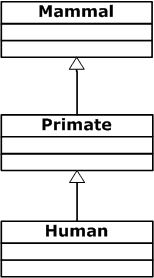
\includegraphics[width=\maxwidth]{images/ref-advanced-topics-refactoring-and-schema-evolution-inheritance-refactoring.png}
\end{center}
In this example you cannot introduce a 'Animal' class above the 'Mammal' or add another class between 'Mammal' and 'Primate'. Also you shouldn't remove an class form the inheritance-hierarchy.

Currently the only possible solution for this refactoring is this.

\begin{enumerate}
\item Create the new hierarchy with different names, preferably in a new package
\item Copy all values from the old classes to the new classes.
\item Redirect all references from existing objects to the new classes.
\end{enumerate}

Take a look at the example to how to add a class into the hierarchy. \hyperref[ref:advanced-topics-refactoring-and-schema-evolution-refactoring-class-hierarchy-inserting-class-into-a-hierarchy]{See "Inserting Class Into A Hierarchy"} (p.~\pageref{ref:advanced-topics-refactoring-and-schema-evolution-refactoring-class-hierarchy-inserting-class-into-a-hierarchy}).

Or how you can remove a class from the inheritance hierarchy. \hyperref[ref:advanced-topics-refactoring-and-schema-evolution-refactoring-class-hierarchy-removing-class-from-a-hierarchy]{See "Removing Class From A Hierarchy"} (p.~\pageref{ref:advanced-topics-refactoring-and-schema-evolution-refactoring-class-hierarchy-removing-class-from-a-hierarchy})

\subsubsection{Removing Class From A Hierarchy}
\label{ref:advanced-topics-refactoring-and-schema-evolution-refactoring-class-hierarchy-removing-class-from-a-hierarchy}

In this example we have a Human class which inherits from the Primate class. Now we want to remove the Primate class and let the Human class inherit directly from the Mammal class.

\begin{center}
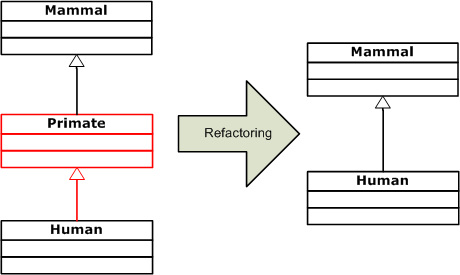
\includegraphics[width=\maxwidth]{images/ref-advanced-topics-refactoring-and-schema-evolution-remove-type-from-hierachy.png}
\end{center}
Unfortunately db4o doesn't support this kind of refactoring. We need to use a work-around. Basically we create a copy of the Human class with the new Inheritance-hierarchy and the copy the existing data over.

\paragraph*{Step by Step}

\begin{enumerate}
\item Create a copy of the Human class, for example HumanNew!
\item Change the inheritance of the HumanNew class to inherit directly from the Mammal class.
\item After that, load all existing Human-instances, copy the values over to HumanNew-instances. Store the HumanNew-instance and delete the old Human-instances
\end{enumerate}

Now the objects have the new inheritance hierarchy. You can delete the old Human class.

\begin{lstlisting}
ObjectSet<Human> allMammals = container.query(Human.class);
for (Human oldHuman : allMammals) {
    HumanNew newHuman = new HumanNew("");
    newHuman.setBodyTemperature(oldHuman.getBodyTemperature());
    newHuman.setIq(oldHuman.getIq());
    newHuman.setName(oldHuman.getName());

    container.store(newHuman);
    container.delete(oldHuman);
}
\end{lstlisting}

{\small\itshape RemoveClassFromHierarchy.java: copy the data from the old type to the new one\par}
\medskip

Note that this example doesn't change existing references from the old instances to the new ones. You need to do this manually as well.

\subsubsection{Inserting Class Into a Hierarchy}
\label{ref:advanced-topics-refactoring-and-schema-evolution-refactoring-class-hierarchy-inserting-class-into-a-hierarchy}

In this example we have a Human class witch inherits from the Mammal class. Now we want to introduce a new Primate class and let the Human class inherit from it.

\begin{center}
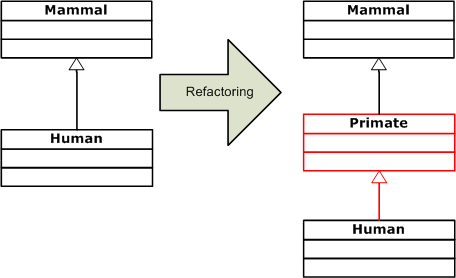
\includegraphics[width=\maxwidth]{images/ref-advanced-topics-refactoring-and-schema-evolution-add-new-type-to-hierachy.png}
\end{center}
Unfortunately db4o doesn't support this kind of refactoring. We need to use a work-around. Basically we create a copy of the Human class with the new Inheritance-hierarchy and the copy the existing data over.

\paragraph*{Step by Step}

\begin{enumerate}
\item Create the new Primate class
\item Create a copy of the Human class, for example HumanNew!
\item Change the HumanNew class to inherit from the new Primate class instead of the Mammal class.
\item After that, load all existing Human-instances, copy the values over to HumanNew instances. Store the HumanNew instance and delete the old Human-instances
\end{enumerate}

Now the objects have the new inheritance hierarchy. You can delete the old Human class.

\begin{lstlisting}
ObjectSet<Human> allMammals = container.query(Human.class);
for (Human oldHuman : allMammals) {
    HumanNew newHuman = new HumanNew("");
    newHuman.setBodyTemperature(oldHuman.getBodyTemperature());
    newHuman.setIq(oldHuman.getIq());
    newHuman.setName(oldHuman.getName());

    container.store(newHuman);
    container.delete(oldHuman);
}
\end{lstlisting}

{\small\itshape AddClassToHierarchy.java: copy the data from the old type to the new one\par}
\medskip

Note that this example doesn't change existing references from the old instances to the new ones. You need to do this manually as well.

\section{Exception Handling}
\label{ref:advanced-topics-exceptions}

A part of the db4o operations is handling possible exceptions. There are two fundamental different exception-types for db4o. The recoverable exceptions and the fatal exceptions.

\subsection*{Recoverable Exceptions}

The recoverable exceptions are all exceptions which don't endanger the consistency of the database. For example if a event callback throws an exception. After a recoverable exception you can continue to work with the object container.

Typical recoverable exceptions are:

\begin{itemize}
\item Exceptions in callbacks.
\item Passing invalid ids to the object container.
\item Unsupported schema-changes.
\item Constraint-violations.
\end{itemize}

\subsection*{Fatal Exceptions}

A fatal exception will immediately shut down the object container without committing anything. This tries to protect the database from damaging itself. Any exception which happens in the db4o core and is not expected and handled is considered as a fatal exception. Because when an exception happens in the db4o-core, it could cause a invalid state in the db4o-core and then cause further errors and lead to database corruption. That's why the policy it the stop immediately any operation after a fatal exception.

Typical fatal recoverable exceptions are:

\begin{itemize}
\item Exceptions related to runtime, like OutOfMemory-exceptions
\item Exceptions related to corrupted database-files.
\end{itemize}

\subsection*{Handle-Exceptions}

Take a look a the list of the most common db4o related exceptions. \hyperref[ref:advanced-topics-exceptions-exception-types]{See "Exception Types"} (p.~\pageref{ref:advanced-topics-exceptions-exception-types}) Handling db4o exceptions is nothing special and complies with regular exception handling.\hyperref[ref:advanced-topics-exceptions-how-to-work-with-db4o-exceptions]{See "How To Work With db4o Exceptions"} (p.~\pageref{ref:advanced-topics-exceptions-how-to-work-with-db4o-exceptions})

\subsection{Exception Types}
\label{ref:advanced-topics-exceptions-exception-types}

Using db4o you will have to deal with db4o-specific exceptions and system exceptions thrown directly out of db4o.

db4o-specific exceptions are unchecked exceptions, which all inherit from a single root class Db4oException.

In Java Unchecked exceptions are inherited from RuntimeExceptions class, while in .NET all exceptions are unchecked.

db4o-exceptions are chained; you can get the cause of the exception using:

Java:

\texttt{db4oException.getCause();}

In order to see all db4o-specific exceptions you can examine the hierarchy of Db4oException class. Currently the following exceptions are available:

\textbf{Db4oException }- db4o exception wrapper: Exceptions occurring during internal processing will be proliferated to the client calling code encapsulated in an exception of this type.

\textbf{BackupInProgressException} - An exception to be thrown when another process is already busy with the backup.

\textbf{ConstraintViolationException }- Base class for all constraint violations.

\textbf{UniqueFieldValueConstraintViolationException} - An exception which will be thrown when the \hyperref[ref:advanced-topics-unique-constraints]{unique constrain} (p.~\pageref{ref:advanced-topics-unique-constraints}) is violated.

\textbf{DatabaseClosedException} - An exception to be thrown when the database was closed or failed to open.

\textbf{DatabaseFileLockedException} - This exception is thrown during any of db4o open calls if the database file is locked by another process.

\textbf{DatabaseMaximumSizeReachedException} - This exception is thrown if the database size is bigger than possible. \hyperref[ref:troubleshoot-increasing-the-maximum-database-file-size]{See "Increasing The Maximum Database File Size"} (p.~\pageref{ref:troubleshoot-increasing-the-maximum-database-file-size})

\textbf{DatabaseReadOnlyException} - This exception is thrown when a write operation was attempted on a database in read-only mode.

\textbf{GlobalOnlyConfigException} - This exception is thrown when you try to change a setting on a open object container, but this setting cannot be changed at runtime.

\textbf{IncompatibleFileFormatException} - An exception to be thrown when an open operation is attempted on a file(database), which format is incompatible with the current version of db4o.

\textbf{InvalidIDException} - an exception to be thrown when an ID format supplied to \#bind or \#getById methods is incorrect.

\textbf{InvalidPasswordException} - This exception is thrown when a client tries to connect to a server with the wrong password.

\textbf{EventException} - This exception is thrown when a exception is thrown in a event callback.

\textbf{OldFormatException} - An exception to be thrown when an old file format was detected and the file could not be open.

\textbf{ReflectException} - An exception to be thrown when a class can not be stored or instantiated by current db4o reflector.

\textbf{ReplicationConflictException} - an exception to be thrown when a conflict occurs and no ReplicationEventListener is specified.

\subsection{How To Work With db4o Exceptions}
\label{ref:advanced-topics-exceptions-how-to-work-with-db4o-exceptions}

Appropriate exception handling will help you to create easy to support systems, saving your time and efforts in the future. The following hints identify important places for exception handling. Take also a look at the list of \hyperref[ref:advanced-topics-exceptions-exception-types]{common db4o exceptions} (p.~\pageref{ref:advanced-topics-exceptions-exception-types}).

\begin{enumerate}
\item Opening a database file can throw a DatabaseFileLockedException.

\begin{lstlisting}
try{
    ObjectContainer container = Db4oEmbedded.openFile("database.db4o");
} catch (DatabaseFileLockedException e){
    // Database is already open!
    // Use another database-file or handle this case gracefully
}
\end{lstlisting}

{\small\itshape ImportantExceptionCases.java: If the database is already open\par}
\medskip
\item Opening a client connection can throw IOException.

\begin{lstlisting}
try{
    final ObjectContainer container = Db4oClientServer.openClient("localhost", 1337, "sa", "sa");

} catch(Db4oIOException e){
    // Couldn't connect to the server.
    // Ask for new connection-settings or handle this case gracefully
}
\end{lstlisting}

{\small\itshape ImportantExceptionCases.java: Cannot connect to the server\par}
\medskip
\item Working with \hyperref[ref:advanced-topics-unique-constraints]{db4o-unique constraints} (p.~\pageref{ref:advanced-topics-unique-constraints}) the commit may throw exceptions when the constraints are violated.

\begin{lstlisting}
container.store(new UniqueId(42));
container.store(new UniqueId(42));
try{
    container.commit();
} catch (UniqueFieldValueConstraintViolationException e){
    // Violated the unique-constraint!
    // Retry with a new value or handle this gracefully
    container.rollback();
}
\end{lstlisting}

{\small\itshape ImportantExceptionCases.java: Violation of the unique constraint\par}
\medskip
\end{enumerate}

\section{db4o Reflection API}
\label{ref:advanced-topics-db4o-reflection-api}

Reflection gives your code access to internal information for classes loaded into the JVM. It allows you to explore the structure of objects at runtime. In the case of reflection metadata is the description of classes and objects within the JVM, including their fields, methods and constructors. It allows the programmer to select target classes at runtime, create new objects, call their methods and operate with the fields.

In order to persist object db4o uses the reflection to read object and store their values. You can exchange this reflector layer in the \hyperref[ref:configuration-common-reflector]{configuration} (p.~\pageref{ref:configuration-common-reflector}).

By default the JdkReflector is used. This reflector also allows you to specify the right class-loader.

\begin{lstlisting}
EmbeddedConfiguration configuration = Db4oEmbedded.newConfiguration();
configuration.common().reflectWith(
        new JdkReflector(Thread.currentThread().getContextClassLoader()));
\end{lstlisting}

{\small\itshape CommonConfigurationExamples.java: Change the reflector\par}
\medskip

It's also possible to use very special class resolving strategy by implementing the JdkLoader-interface. For example when you want to look up classes in multiple class loaders.

\begin{lstlisting}
EmbeddedConfiguration configuration = Db4oEmbedded.newConfiguration();

JdkLoader classLookUp = new ClassLoaderLookup(
        Thread.currentThread().getContextClassLoader(),
        new URLClassLoader(new URL[]{new URL("file://./some/other/location")}));
configuration.common().reflectWith(new JdkReflector(classLookUp));

ObjectContainer container = Db4oEmbedded.openFile("database.db4o");
\end{lstlisting}

{\small\itshape CommonConfigurationExamples.java: Complex class loader scenario\par}
\medskip

\begin{lstlisting}
public class ClassLoaderLookup implements JdkLoader {
    private final List<ClassLoader> classLoaders;

    ClassLoaderLookup(ClassLoader...classLoaders) {
        this.classLoaders = Arrays.asList(classLoaders);
    }

    ClassLoaderLookup(Collection<ClassLoader> classLoaders) {
        this.classLoaders = new ArrayList<ClassLoader>(classLoaders);
    }

    @Override
    public Class loadClass(String className) {
        for (ClassLoader loader : classLoaders) {
            Class<?> theClass = null;
            try {
                theClass = loader.loadClass(className);
                return theClass;
            } catch (ClassNotFoundException e) {
                // first check the other loaders
            }
        }
        throw new RuntimeException(new ClassNotFoundException(className));
    }

    @Override
    public Object deepClone(Object o) {
        return new ClassLoaderLookup(classLoaders);
    }
}
\end{lstlisting}

{\small\itshape ClassLoaderLookup.java: Complex class loader scenario\par}
\medskip

If you need some special treatment you can create you're own reflector implementation. \hyperref[ref:advanced-topics-db4o-reflection-api-creating-your-own-reflector]{See "Creating your own reflector"} (p.~\pageref{ref:advanced-topics-db4o-reflection-api-creating-your-own-reflector})

db4o has also a generic reflector which can deal with stored objects without using the original class. \hyperref[ref:advanced-topics-db4o-reflection-api-genericreflector]{See "GenericReflector"} (p.~\pageref{ref:advanced-topics-db4o-reflection-api-genericreflector})

\subsection{Creating your own reflector}
\label{ref:advanced-topics-db4o-reflection-api-creating-your-own-reflector}

By default db4o uses the JdkReflector . As alternative you can create your own reflector and use it with db4o. In order to do so you need to implement the Reflector interface. And then pass an instance of your implementation to db4o.

Here's an example of a logging reflector. Its only difference from standard reflector is that information about loaded classes is outputted to console:

\begin{lstlisting}
class LoggerReflector implements Reflector{
    private final Reflector readReflector;

    public LoggerReflector() {
        this(new JdkReflector(Thread.currentThread().getContextClassLoader()));
    }

    public LoggerReflector(Reflector readReflector) {
        this.readReflector = readReflector;
    }

    @Override
    public void configuration(ReflectorConfiguration reflectorConfiguration) {
        readReflector.configuration(reflectorConfiguration);
    }

    @Override
    public ReflectArray array() {
        return readReflector.array();
    }

    @Override
    public ReflectClass forClass(Class aClass) {
        System.out.println("Reflector.forClass("+aClass+")");
        return readReflector.forClass(aClass);
    }

    @Override
    public ReflectClass forName(String className) {
        System.out.println("Reflector.forName("+className+")");
        return readReflector.forName(className);
    }

    @Override
    public ReflectClass forObject(Object o) {
        System.out.println("Reflector.forObject("+o+")");
        return readReflector.forObject(o);
    }

    @Override
    public boolean isCollection(ReflectClass reflectClass) {
        return readReflector.isCollection(reflectClass);
    }

    @Override
    public void setParent(Reflector reflector) {
        readReflector.setParent(reflector);
    }

    @Override
    public Object deepClone(Object o) {
        return new LoggerReflector((Reflector) readReflector.deepClone(o));
    }
}
\end{lstlisting}

{\small\itshape ReflectorExamples.java: Logging reflector\par}
\medskip

\subsection{GenericReflector}
\label{ref:advanced-topics-db4o-reflection-api-genericreflector}

db4o uses reflection internally for persisting and instantiating user objects. Reflection helps db4o to manage classes in a general way while saving. It also makes instantiation of objects using class name possible. However db4o reflection API can also work on generic objects when a class information is not available.

db4o uses a generic reflector as a decorator around specific reflector. The generic reflector is set when an object container is opened. All subsequent reflector calls are routed through this decorator.

The generic reflector keeps list of known classes in memory. When the generic reflector is called, it first checks its list of known classes. If the class cannot be found, the task is transferred to the delegate reflector. If the delegate fails as well, generic objects are created, which hold simulated "field values" in an array of objects.

Generic reflector makes possible the following use cases:

\begin{itemize}
\item Running a db4o server without deploying application classes.
\item Easier access to stored objects where classes or fields are not available.
\item Building interfaces to db4o from any programming language.
\end{itemize}

One of the live use cases is the ObjectManager, which uses the generic reflector to read C\# objects from Java.

The generic reflector is automatically used when the class of a stored object is not found.

\section{Runtime Statistics}
\label{ref:advanced-topics-runtime-statistics}

The db4o runtime statistics is a monitoring feature allowing to collect various important runtime data. This data can be crucial in resolving performance issues, analyzing usage patterns, predicting resource bottlenecks etc. Runtime Statistics can be collected both in the application testing stage and in an application deployed to production system. In the first case this data can help to estimate hardware requirements and analyze the stability of the system. In the latter case, the data can be used to fine-tune performance, find problems and fix bugs. Take a look how you install the statistics and monitor them.

\subsection*{Install And Monitor}

On the Java platform all runtime statistics are published through the JMX interface. This means that you can use any JMX client to monitor the statistics. \hyperref[ref:advanced-topics-runtime-statistics-install-and-monitor]{See "Install and Monitor"} (p.~\pageref{ref:advanced-topics-runtime-statistics-install-and-monitor})

\subsection*{Available Statistics}

Currently following statistics are available.

\begin{itemize}
\item \hyperref[ref:advanced-topics-runtime-statistics-monitor-queries]{Query Monitoring} (p.~\pageref{ref:advanced-topics-runtime-statistics-monitor-queries}): Monitor how queries behave and perform.
\item \hyperref[ref:advanced-topics-runtime-statistics-monitor-object-lifecycle]{Object Lifecycle Monitoring} (p.~\pageref{ref:advanced-topics-runtime-statistics-monitor-object-lifecycle}): Monitor how many objects are stored, deleted and activated.
\item \hyperref[ref:advanced-topics-runtime-statistics-monitor-io]{IO Monitoring} (p.~\pageref{ref:advanced-topics-runtime-statistics-monitor-io}): Monitor the IO-operations of db4o.
\item \hyperref[ref:advanced-topics-runtime-statistics-monitor-network]{Network Monitoring} (p.~\pageref{ref:advanced-topics-runtime-statistics-monitor-network}): Monitor the network operations of db4o.
\item \hyperref[ref:advanced-topics-runtime-statistics-monitor-reference-system]{Reference System Monitoring} (p.~\pageref{ref:advanced-topics-runtime-statistics-monitor-reference-system}): Monitor db4o's reference system.
\end{itemize}

\subsection{Install and Monitor}
\label{ref:advanced-topics-runtime-statistics-install-and-monitor}

On the Java platform all runtime statistics are published through the JMX interface. This means that you can use any JMX client to monitor the statistics.

\subsubsection*{Installing the Monitoring Support}

The first thing we need to do is to add the monitoring support to the db4o configuration. The monitoring-support are in \hyperref[ref:dependency-overview]{the optional-jar s} (p.~\pageref{ref:dependency-overview}). So you need to add those for the monitoring support.

Monitoring adds a small overhead to the regular db4o operations. Therefore the monitoring support is distributed across different monitoring options, so that you can add only the options you need.

Currently following options are available:

\begin{itemize}
\item \hyperref[ref:advanced-topics-runtime-statistics-monitor-queries]{Query Monitoring} (p.~\pageref{ref:advanced-topics-runtime-statistics-monitor-queries}): Monitor how queries behave and perform.
\item \hyperref[ref:advanced-topics-runtime-statistics-monitor-object-lifecycle]{Object Lifecycle Monitoring} (p.~\pageref{ref:advanced-topics-runtime-statistics-monitor-object-lifecycle}): Monitor how many objects are stored, deleted and activated.
\item \hyperref[ref:advanced-topics-runtime-statistics-monitor-io]{IO Monitoring} (p.~\pageref{ref:advanced-topics-runtime-statistics-monitor-io}): Monitor the IO-operations of db4o.
\item \hyperref[ref:advanced-topics-runtime-statistics-monitor-network]{Network Monitoring} (p.~\pageref{ref:advanced-topics-runtime-statistics-monitor-network}): Monitor the network operations of db4o.
\item \hyperref[ref:advanced-topics-runtime-statistics-monitor-reference-system]{Reference System Monitoring} (p.~\pageref{ref:advanced-topics-runtime-statistics-monitor-reference-system}): Monitor db4o's reference system.
\end{itemize}

\subsubsection*{Monitor With JConsole}

As said, the statistics are published through the JMX-interface (Java Management Extensions). Therefore you can use any JMX-client to monitor db4o. The JDK brings its own JMX-client with it: The \href{http://java.sun.com/javase/6/docs/technotes/guides/visualvm/intro.html}{JConsole}-application is located in the bin-folder of the JDK-installation. Start the JConsole and connect your running db4o application. Then you will find the db4o related readings on the "MBeans" tab. In the treeview on the left, you will see "com.db4o.monitoring".

Below this tree node you will find all open ObjectContainers that have JMX monitoring enabled. For each of them the respective runtime statistics categories will be listed. If you select the "Attributes" node for any of them, the corresponding set of attribute values will be shown along with their most recent reading.

By double clicking on the number value a graph will be displayed.

Some Monitoring-Nodes also provide notifications. You can subscribe to this notifications. In the categories where the "Notifications" node is visible, you can select it and click "Subscribe" on the bottom right. For example we provide notifications about unoptimized native queries and about class index scans.

\begin{center}
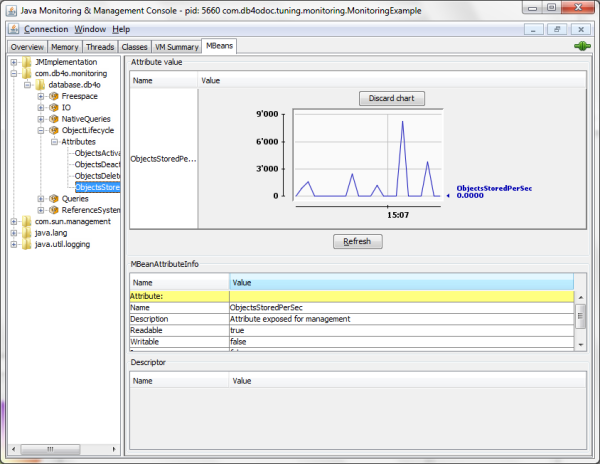
\includegraphics[width=\maxwidth]{images/ref-advanced-topics-runtime-statistics-jconsole.png}
\end{center}
\subsection{Monitoring Queries}
\label{ref:advanced-topics-runtime-statistics-monitor-queries}

You can monitor queries to find out more about the runtime behavior of your application.

\subsubsection*{Configure the Query Monitoring Support}

First you need to add the monitoring support to the db4o configuration. There are two separate items. The QueryMonitoringSupport will monitor the very basic query operations. The NativeQueryMonitoringSupport adds additional statistics about  native queries.

\begin{lstlisting}
configuration.common().add(new QueryMonitoringSupport());
configuration.common().add(new NativeQueryMonitoringSupport());
\end{lstlisting}

{\small\itshape QueryMonitoring.java: Add query monitoring\par}
\medskip

\subsubsection*{The Query Statistics}

\textbf{AverageQueryExecutionTime} : Tells you how long on average a query takes to execute. Of course this heavily depends on the complexity of the queries. However if this number is high, you maybe should improve you query-performance. For example by adding additional indexes. \hyperref[ref:basics-indexing]{See "Indexing"} (p.~\pageref{ref:basics-indexing})

\textbf{ClassIndexScansPerSecond}: Tells you the number of queries which required to scan through all objects. This means that a query couldn't use a field index and therefore required to go through all objects. This is of course slow. You should try to keep this number low by adding the right indexes on fields. \hyperref[ref:basics-indexing]{See "Indexing"} (p.~\pageref{ref:basics-indexing})

\textbf{QueriesPerSecond}: Tells you how many queries run per second.

\textbf{Loaded From Class Index Notifications}: The query statistics can notify you every time a query used the class-index and couldn't utilize a field index. You should try to avoid loading by class index by adding the right indexes on fields. \hyperref[ref:basics-indexing]{See "Indexing"} (p.~\pageref{ref:basics-indexing})

\subsubsection*{The Native Query Statistics}

\textbf{NativeQueriesPerSecond}: Tells you how many native queries per second run.

\textbf{UnoptimizedNativeQueriesPerSecond}: Tells you how many unoptimized native queries run per second. Such queries need to instantiate all objects which is a slow operation. If this number is high, you should try to simplify your queries.

\textbf{Native Query Not Optimized Notifications}: The native query statistics can notify you every time a query couldn't be optimized. You should try to avoid such queries. Try to simplify the native query or fall back to SODA-queries.

\subsection{Monitor Object Lifecycle}
\label{ref:advanced-topics-runtime-statistics-monitor-object-lifecycle}

You can monitor the object lifecycle statistics of db4o to find out more about the runtime behavior of your application.

\subsubsection*{Configure the Object Lifecycle Monitoring Support}

In order to monitor the object lifecycle statistics, you need to add the monitoring support to the configuration.

\begin{lstlisting}
configuration.common().add(new ObjectLifecycleMonitoringSupport());
\end{lstlisting}

{\small\itshape ObjectLifecycleMonitoring.java: Monitor the object lifecycle statistics\par}
\medskip

\subsubsection*{The Object Lifecycle Statistics}

\textbf{ObjectsActivatedPerSec}: Tells you how many objects are \hyperref[ref:basics-activation]{activated} (p.~\pageref{ref:basics-activation}) per second. Activation can consume a lot of time for complex object graphs. If there's a lot of time spend with activating objects, you may want to reduce the amount of activated objects. One of the best way to activate only the minimum set of objects is to use \hyperref[ref:basics-activation-concept-transparent-activation-framework]{transparent activation} (p.~\pageref{ref:basics-activation-concept-transparent-activation-framework}).

\textbf{ObjectsDeactivatedPerSec}: Tells you how many objects are deactivate per second.

\textbf{ObjectsDeletedPerSec}: Tells you how many objects are deleted per second.

\textbf{ObjectsStoredPerSec}: Tells you how many objects are stored per second.

\subsection{Monitor IO}
\label{ref:advanced-topics-runtime-statistics-monitor-io}

You can monitor the IO-operations of db4o to find out more about the runtime behavior of your application.

\subsubsection*{Configure the IO Monitoring Support}

In order to monitor the IO activities of db4o you need to configure the IO monitoring support.

\begin{lstlisting}
configuration.common().add(new IOMonitoringSupport());
\end{lstlisting}

{\small\itshape IOMonitoring.java: Add IO-Monitoring\par}
\medskip

\subsubsection*{The IO Statistics}

\textbf{BytesReadPerSecond}: Tells you how many bytes are read per second from the disk.

\textbf{BytesWrittenPerSecond}: Tells you how many bytes are written to disk per second.

\textbf{ReadsPerSecond}: Tells how many read requests are issues per second.

\textbf{SyncsPerSecond}: Tells you how many sync-operations are done per second. The sync-operation is a part of the commit-process. I forces the runtime and operating system to flush all buffers to the disk to ensure that the data are safely stored. The sync operation is normally a costly operation, since it need to wait on the physical disk to finish all write operations

.\textbf{WritesPerSecond}: Tells you how may write requests are issued per second.

\subsection{Monitor Freespace}
\label{ref:advanced-topics-runtime-statistics-monitor-freespace}

You can monitor the freespace-manager to find out more about the runtime behavior of your application.

\subsubsection*{Configure the Freespace Monitoring Support}

To monitor the freespace manager you need to add the monitoring support to the db4o configuration.

\begin{lstlisting}
configuration.common().add(new FreespaceMonitoringSupport());
\end{lstlisting}

{\small\itshape FreespaceMonitoring.java: Monitor the free-space system\par}
\medskip

\subsubsection*{The Freespace Statistics}

\textbf{AverageSlotSize}: Tells you how big the average slot is. When you store larger objects, they need larger slots to fit it.

\textbf{ReusedSlotsPerSecond}: Tells you how many slots can be reused. When an object is deleted or modified, its old slot is released and can be reused. If you modify and delete a lot of objects, but the slots cannot be reused, then the database-file will fragment.

When this number is low but the free-space increases and increases then you have a fragmentation issue. \hyperref[ref:advanced-topics-defragment]{Defragment} (p.~\pageref{ref:advanced-topics-defragment}) your database. Use the \hyperref[ref:configuration-id-system]{btree-id-system.} (p.~\pageref{ref:configuration-id-system})

\textbf{SlotCount}: Tells you how many slots are used by the database. As more and more objects are stored, the slot count will increase.

\textbf{TotalFreespace}: Tells you how much freespace there is in the database-file.A hight free-space number with a low reused slots number indicates database fragmentation. \hyperref[ref:advanced-topics-defragment]{Defragment} (p.~\pageref{ref:advanced-topics-defragment}) your database. Use the \hyperref[ref:configuration-id-system]{btree-id-system.} (p.~\pageref{ref:configuration-id-system})

\subsection{Monitor Network}
\label{ref:advanced-topics-runtime-statistics-monitor-network}

You can monitor the network-operations of db4o in client-server mode.

\subsubsection*{Configure the Network Monitoring Support}

First you need to add the monitoring support to the db4o configuration. The network monitoring support is in two separate configuration-items. The NetworkingMonitoringSupport can be used on the server and client to monitor the network statistics.

\begin{lstlisting}
configuration.common().add(new NetworkingMonitoringSupport());
\end{lstlisting}

{\small\itshape CSMonitoring.java: Add the network monitoring support\par}
\medskip

The ClientConnectionsMonitoringSupport can be added to the db4o server to monitor the connected clients.

\begin{lstlisting}
configuration.addConfigurationItem(new ClientConnectionsMonitoringSupport());
\end{lstlisting}

{\small\itshape CSMonitoring.java: Add the client connections monitoring support\par}
\medskip

\subsubsection*{The Network Statistics}

\textbf{BytesReceivedPerSecond}: Tells you how many bytes this client or server has receives per second.

\textbf{BytesSentPerSecond}: Tells you how many bytes this client or server sends per second.

\textbf{MessagesSentPerSecond}: Tells you how many messages this client or server sends per second.

\textbf{ConnectedClientCount}: Tells you how many clients are connected to this server.

\subsection{Monitor Reference System}
\label{ref:advanced-topics-runtime-statistics-monitor-reference-system}

You can monitor the \hyperref[ref:basics-indentity-concept-reference-cache]{reference-system} (p.~\pageref{ref:basics-indentity-concept-reference-cache}) to find out more about the runtime behavior of your application. The reference-system ensures that each object has only one in memory representation.

\subsubsection*{Configure the Reference System Monitoring Support}

First you need to add the monitoring support to the db4o configuration.

\begin{lstlisting}
configuration.common().add(new ReferenceSystemMonitoringSupport());
\end{lstlisting}

{\small\itshape ReferenceSystemMonitoring.java: Add reference system monitoring\par}
\medskip

\subsubsection*{The Freespace Statistics}

\textbf{ObjectReferenceCount}: Tells you how many references are currently hold in the reference-system. By default db4o uses weak references to objects. If this count is very high, you might hold unnecessary references to persisted objects in your application.

\section{Diagnostics}
\label{ref:advanced-topics-diagnostics}

The db4o engine provides user with a special mechanism showing runtime diagnostics information. Diagnostics can be switched on in the configuration before opening the database file:

The DiagnosticListener is a callback interface tracking diagnostic messages from different parts of the system.

\begin{lstlisting}
EmbeddedConfiguration configuration = Db4oEmbedded.newConfiguration();
configuration.common().diagnostic().addListener(new DiagnosticToConsole());
\end{lstlisting}

{\small\itshape CommonConfigurationExamples.java: Add a diagnostic listener\par}
\medskip

\subsection*{Built-in Listeners}

There are two build in listeners, which print the output to the console

\begin{itemize}
\item DiagnosticToConsole:Prints diagnostic messages to the console.
\item DiagnosticToTrace: Only on .NET, prints diagnostic messages to the debug output window.
\end{itemize}

\subsection*{Messages-Types}

Every diagnostic message is represented by it's own type. You can filter the messages by checking for certain instances. Take a look how you can filter for \hyperref[ref:advanced-topics-diagnostics-diagnostic-messages-filter]{certain messages.} (p.~\pageref{ref:advanced-topics-diagnostics-diagnostic-messages-filter})

\begin{itemize}
\item \textbf{MissingClass}: Notifies you that a class couldn't be found. You should add that class in order to avoid problems. If you've renamed the class, you \hyperref[ref:advanced-topics-refactoring-and-schema-evolution]{should rename} (p.~\pageref{ref:advanced-topics-refactoring-and-schema-evolution}) it in the database or add \hyperref[ref:configuration-common-alias]{an alias} (p.~\pageref{ref:configuration-common-alias}).
\item \textbf{DefragmentRecommendation}: Notifies you that you should consider to \hyperref[ref:advanced-topics-defragment]{defragment} (p.~\pageref{ref:advanced-topics-defragment}) the database.
\item \textbf{LoadedFromClassIndex}: Notifies you that db4o couldn't use a field-index to perform a query. This means that the query runs extremely slow on larger data sets. Consider adding a \hyperref[ref:basics-indexing]{field-index} (p.~\pageref{ref:basics-indexing}).
\item \textbf{DescendIntoTranslator}: Means that you a query couldn't be optimized, because the query touches a class \hyperref[ref:advanced-topics-type-handling-translators]{with a translator} (p.~\pageref{ref:advanced-topics-type-handling-translators}). Therefore the query runs slow. You should consider working without a translator or changing the query.
\item \textbf{ClassHasNoFields}: You stored a class which has no fields. Even when the class has no fields it need to maintain its class index and needs to be stored. So it adds overhead for storing 'empty' objects. You should consider removing the empty class.
\item \textbf{DeletionFailed}: db4o failed to delete a object from the database.
\item \textbf{UpdateDepthGreaterOne}: You have configured a update depth greater one. A large update depth slows down updates significantly. Consider reducing the update-depth and use another strategies to update objects correctly, like \hyperref[ref:basics-update-concept-transparent-persistence]{transparent persistence} (p.~\pageref{ref:basics-update-concept-transparent-persistence}).
\item \textbf{NativeQueryNotOptimized}: A native query couldn't be optimized. An unoptimized query runs significantly slower than a optimized query. Consider to simplify you're query.
\item \textbf{NativeQueryOptimizerNotLoaded}: Couldn't load the native query optimizer. Ensure that all required jar are added to your application.
\item \textbf{NotTransparentActivationEnabled}: Notifies you when a class doesn't support transparent activation. Such object need to be fully activated and slow down the activation process.
\item \textbf{ObjectFieldDoesNotExist}: A query uses a object-field which doesn't exist. Check you're queries to use only exising fields.
\end{itemize}

\subsection{Diagnostic Messages Filter}
\label{ref:advanced-topics-diagnostics-diagnostic-messages-filter}

The standard listeners can potentially produce quite a lot of messages. By writing your own DiagnosticListener you can filter that information.

On the stage of application tuning you can be interested in optimizing performance through indexing. Diagnostics can help you with giving information about queries that are running on un-indexed fields. By having this information you can decide which queries are frequent and heavy and should be indexed, and which have little performance impact and do not need an index. Field indexes dramatically improve query performance but they may considerably reduce storage and update performance.

In order to get rid of all unnecessary diagnostic information and concentrate on indexes let's create special diagnostic listener:

\begin{lstlisting}
private static class DiagnosticFilter implements DiagnosticListener{
    private final Set<Class> filterFor;
    private final DiagnosticListener delegate;

    private DiagnosticFilter(DiagnosticListener delegate,Class<? extends Diagnostic>...filterFor) {
        this.delegate = delegate;
        this.filterFor = new HashSet<Class>(Arrays.asList(filterFor));
    }

    public void onDiagnostic(Diagnostic diagnostic) {
        Class<?> type = diagnostic.getClass();
        if(filterFor.contains(type)){
            delegate.onDiagnostic(diagnostic);
        }
    }
}
\end{lstlisting}

{\small\itshape DiagnosticsExamples.java: A simple message filter\par}
\medskip

After that we can use the filter-listener. It takes two arguments. The first one is a regular listener, the second is a list of all messages which are passed through.

\begin{lstlisting}
EmbeddedConfiguration configuration = Db4oEmbedded.newConfiguration();
configuration.common().diagnostic()
        .addListener(new DiagnosticFilter(new DiagnosticToConsole(), LoadedFromClassIndex.class));
\end{lstlisting}

{\small\itshape DiagnosticsExamples.java: Filter for unindexed fields\par}
\medskip


% Converted from reference/DB4OFlare (MadCap Flare, Java target)

\chapter{Configuration}
\label{ref:configuration}

db4o is configured by its configuration API. The configuration allows you to adjust db4o to your scenarios.

\section*{Configure db4o}

In order to configure db4o, you need to create a new configuration-instance and set the desired settings on it. After that, you pass the configuration-instance to the object-container factory.

Note that you cannot share a configuration-instance. For each object-container you create, you need to pass in a new configuration-instance. It's recommended to create a method which will return a new configuration instance on request:

\section*{Embedded-Configuration}

For an embedded container you can configure the \hyperref[ref:configuration-common-configuration]{common} (p.~\pageref{ref:configuration-common-configuration})-, \hyperref[ref:configuration-file-configuration]{file} (p.~\pageref{ref:configuration-file-configuration})- and \hyperref[ref:configuration-id-system]{id-system} (p.~\pageref{ref:configuration-id-system})-configuration.

\begin{lstlisting}
EmbeddedConfiguration configuration = Db4oEmbedded.newConfiguration();
// change the configuration...
ObjectContainer container = Db4oEmbedded.openFile(configuration, "database.db4o");
\end{lstlisting}

\section*{Server-Configuration}

For an server you can configure the \hyperref[ref:configuration-common-configuration]{common} (p.~\pageref{ref:configuration-common-configuration})-, \hyperref[ref:configuration-file-configuration]{file} (p.~\pageref{ref:configuration-file-configuration})-, \hyperref[ref:configuration-network-configuration]{networking} (p.~\pageref{ref:configuration-network-configuration})-, \hyperref[ref:configuration-server-configuration]{server} (p.~\pageref{ref:configuration-server-configuration})- and \hyperref[ref:configuration-id-system]{id-system} (p.~\pageref{ref:configuration-id-system})-configuration.

\begin{lstlisting}
ServerConfiguration configuration = Db4oClientServer.newServerConfiguration();
// change the configuration...
ObjectServer server = Db4oClientServer.openServer(configuration, "database.db4o", 1337);
\end{lstlisting}

\section*{Client-Configuration}

For an client you can configure the \hyperref[ref:configuration-common-configuration]{common} (p.~\pageref{ref:configuration-common-configuration})-, \hyperref[ref:configuration-network-configuration]{networking} (p.~\pageref{ref:configuration-network-configuration})-, \hyperref[ref:configuration-client-configuration]{client} (p.~\pageref{ref:configuration-client-configuration})- and \hyperref[ref:configuration-id-system]{id-system} (p.~\pageref{ref:configuration-id-system})-configuration.

\begin{lstlisting}
ClientConfiguration configuration = Db4oClientServer.newClientConfiguration();
// change the configuration...
ObjectContainer container = Db4oClientServer.openClient(configuration, "localhost", 1337, "user", "pwd");
\end{lstlisting}

\section*{Configuration Is Not Persistent}

The db4o configuration is not persistent with a few exception. This means that you need to configure db4o each time you create a object-container instance.

\section*{Configuration in Client/Server-Mode}

For using db4o in client/server mode it is recommended to use the same configuration on the server and on the client. To set this up nicely it makes sense to create one application class with one method that returns the required configuration and to deploy this class both to the server and to all clients.

\section*{Configuration-Settings Overview}

The configuration-settings which are common across -client, embedded and db4o-server are summed up here: \hyperref[ref:configuration-common-configuration]{See "Common Configuration"} (p.~\pageref{ref:configuration-common-configuration})

\section{Common Configuration}
\label{ref:configuration-common-configuration}

The common-configuration applies to the embedded-, client- and the server-mode of db4o. All the common configuration is accessible via the common-getter on the configuration-object.

\subsection*{Overview}

Here's a overview over all common configuration-settings which you can change:

{\small
\begin{longtable}{|p{\dimexpr(\linewidth-4\arrayrulewidth)*1/3-2\tabcolsep\relax}|p{\dimexpr(\linewidth-4\arrayrulewidth)*1/3-2\tabcolsep\relax}|p{\dimexpr(\linewidth-4\arrayrulewidth)*1/3-2\tabcolsep\relax}|}
\hline
 & Same in C/S\footnote{This setting needs to be the same on the server and all clients.} & Can not change \footnote{This setting has to be set the first time when the database is created. You cannot change is for an existing database.} \\ \hline
\textbf{\hyperref[ref:configuration-common-activation-depth]{ActivationDepth} (p.~\pageref{ref:configuration-common-activation-depth})}: Change globally the activation-depth. &  &  \\ \hline
\textbf{\hyperref[ref:configuration-common-alias]{Aliases} (p.~\pageref{ref:configuration-common-alias})}: Configure aliases for class and package-names. &  &  \\ \hline
\textbf{\hyperref[ref:configuration-common-updating-db4o-file-format]{AllowVersionUpdates} (p.~\pageref{ref:configuration-common-updating-db4o-file-format})}: Allow/Disallow to update the database-format. & Yes &  \\ \hline
\textbf{\hyperref[ref:configuration-common-automatic-shutdown]{AutomaticShutDown} (p.~\pageref{ref:configuration-common-automatic-shutdown})}: Close the database when the application exits. &  &  \\ \hline
\textbf{\hyperref[ref:configuration-common-btree-node-size]{BTreeNodeSize} (p.~\pageref{ref:configuration-common-btree-node-size})}: Tune the size of the B-tree-node which are used for the indexes. &  &  \\ \hline
\textbf{\hyperref[ref:configuration-common-no-callbacks]{Callbacks} (p.~\pageref{ref:configuration-common-no-callbacks})}: Turn object-callbacks on an off. &  &  \\ \hline
\textbf{\hyperref[ref:configuration-common-calling-constructors]{CallConstructors} (p.~\pageref{ref:configuration-common-calling-constructors})}: Use or bypass the constructor for creating objects. &  &  \\ \hline
\textbf{\hyperref[ref:configuration-common-no-schema-changes]{DetectSchemaChanges} (p.~\pageref{ref:configuration-common-no-schema-changes})}: Disable/Enable schema changes detection. &  &  \\ \hline
\textbf{\hyperref[ref:configuration-common-diagnostics]{Diagnostic} (p.~\pageref{ref:configuration-common-diagnostics})}: Add diagnostic-listeners. &  &  \\ \hline
\textbf{\hyperref[ref:configuration-common-exceptionsonnotstorable]{ExceptionsOnNotStorable} (p.~\pageref{ref:configuration-common-exceptionsonnotstorable})}: Enable/Disable exceptions on not storable objects. &  &  \\ \hline
\textbf{\hyperref[ref:configuration-common-intern-strings]{InternStrings} (p.~\pageref{ref:configuration-common-intern-strings})}: Will call the intern-method on the retrieved strings. &  &  \\ \hline
\textbf{\hyperref[ref:configuration-common-mark-transient]{MarkTransient} (p.~\pageref{ref:configuration-common-mark-transient})}: Configure a Annotation for marking fields as transient. &  &  \\ \hline
\textbf{\hyperref[ref:configuration-common-message-level]{MessageLevel} (p.~\pageref{ref:configuration-common-message-level})}: Configure the logging-message level. &  &  \\ \hline
\textbf{\hyperref[ref:configuration-common-name-provider]{NameProvider} (p.~\pageref{ref:configuration-common-name-provider})}: Configure the toString() value of the object-container. &  &  \\ \hline
\textbf{\hyperref[ref:configuration-common-max-stack-size]{MaxStackSize} (p.~\pageref{ref:configuration-common-max-stack-size})}: Configure how many recursive operations are executed directly on the stack. &  &  \\ \hline
\textbf{\hyperref[ref:configuration-objectclass-configuration]{ObjectClass} (p.~\pageref{ref:configuration-objectclass-configuration})}: Configure class-specific settings. &  &  \\ \hline
\textbf{\hyperref[ref:configuration-common-disable-optimize-nq]{OptimizeNativeQueries} (p.~\pageref{ref:configuration-common-disable-optimize-nq})}: Enable runtime query optimization. &  &  \\ \hline
\textbf{\hyperref[ref:configuration-common-out-stream]{OutStream} (p.~\pageref{ref:configuration-common-out-stream})}: Configure the log message output stream &  &  \\ \hline
\textbf{\hyperref[ref:configuration-common-query-modes]{Queries} (p.~\pageref{ref:configuration-common-query-modes})}: Configure query behaviors &  &  \\ \hline
\textbf{\hyperref[ref:advanced-topics-db4o-reflection-api]{ReflectWith} (p.~\pageref{ref:advanced-topics-db4o-reflection-api})}: Configure a reflector. &  &  \\ \hline
\textbf{\hyperref[ref:advanced-topics-type-handling-typehandlers]{RegisterTypeHandler} (p.~\pageref{ref:advanced-topics-type-handling-typehandlers})}: Register a new TypeHandler. & Required &  \\ \hline
\textbf{\hyperref[ref:configuration-common-string-encoding]{StringEncoding} (p.~\pageref{ref:configuration-common-string-encoding})}: Configure the string-encoding. & Required & Yes \\ \hline
\textbf{\hyperref[ref:configuration-common-no-test-instances]{TestConstructors} (p.~\pageref{ref:configuration-common-no-test-instances})}: Configure if db4o checks for valid constructors. &  &  \\ \hline
\textbf{\hyperref[ref:configuration-common-update-depth]{UpdateDepth} (p.~\pageref{ref:configuration-common-update-depth})}: Change the update-depth. &  &  \\ \hline
\textbf{\hyperref[ref:configuration-common-weak-reference-collection-interval]{WeakReferenceCollectionInterval} (p.~\pageref{ref:configuration-common-weak-reference-collection-interval})}: Change the weak-reference cleanup interval. Default setting is 1000 milliseconds. &  &  \\ \hline
\textbf{\hyperref[ref:configuration-common-disable-weak-references]{WeakReferences} (p.~\pageref{ref:configuration-common-disable-weak-references})}: Enable/disable weak references. &  &  \\ \hline
\end{longtable}}

\subsection*{Additional Configuration Items}

There are additional configuration items which add for additional features. You can add then on the common-configuration. For example to enable transparent persistence you add the TransparentPersistenceSupport configuration item. Take a look a the available configuration items. \hyperref[ref:configuration-common-configuration-items]{See "Common Configuration Items"} (p.~\pageref{ref:configuration-common-configuration-items})

\subsection{Common Configuration Items}
\label{ref:configuration-common-configuration-items}

Configuration items add special capability to the system. Here's a list of all configuration items available.

\subsubsection*{TransparentActivationSupport}

Support for transparent activation. \hyperref[ref:basics-activation-concept-transparent-activation-framework]{See "Transparent Activation Framework"} (p.~\pageref{ref:basics-activation-concept-transparent-activation-framework})

\subsubsection*{TransparentPersistenceSupport}

Support for transparent persistence. \hyperref[ref:basics-update-concept-transparent-persistence]{See "Transparent Persistence"} (p.~\pageref{ref:basics-update-concept-transparent-persistence})

\subsubsection*{UniqueFieldValueConstraint}

Set up unique Field constraints. \hyperref[ref:advanced-topics-unique-constraints]{See "Unique Constraints"} (p.~\pageref{ref:advanced-topics-unique-constraints})

\subsubsection*{BigMathSupport}

Add support for the BigDecimal and BigInteger classes. \hyperref[ref:advanced-topics-type-handling-bigmath]{See "BigMath"} (p.~\pageref{ref:advanced-topics-type-handling-bigmath})

\subsubsection*{FreespaceMonitoringSupport}

Enables you to monitor the free-space-manager. \hyperref[ref:advanced-topics-runtime-statistics]{See "Runtime Statistics"} (p.~\pageref{ref:advanced-topics-runtime-statistics})

\subsubsection*{IOMonitoringSupport}

Enables you to monitor the IO-activity of db4o. \hyperref[ref:advanced-topics-runtime-statistics]{See "Runtime Statistics"} (p.~\pageref{ref:advanced-topics-runtime-statistics})

\subsubsection*{NativeQueryMonitoringSupport}

Enables you to monitor the native queries. \hyperref[ref:advanced-topics-runtime-statistics]{See "Runtime Statistics"} (p.~\pageref{ref:advanced-topics-runtime-statistics})

\subsubsection*{NetworkingMonitoringSupport}

Enables you to monitor the network activity of db4o. \hyperref[ref:advanced-topics-runtime-statistics]{See "Runtime Statistics"} (p.~\pageref{ref:advanced-topics-runtime-statistics})

\subsubsection*{ObjectLifecycleMonitoringSupport}

Enables you to monitor the object lifecycles. \hyperref[ref:advanced-topics-runtime-statistics]{See "Runtime Statistics"} (p.~\pageref{ref:advanced-topics-runtime-statistics})

\subsubsection*{QueryMonitoringSupport}

Enables you to monitor db4o queries. \hyperref[ref:advanced-topics-runtime-statistics]{See "Runtime Statistics"} (p.~\pageref{ref:advanced-topics-runtime-statistics})

\subsubsection*{ReferenceSystemMonitoringSupport}

Enables you to monitor db4o's reference system. \hyperref[ref:advanced-topics-runtime-statistics]{See "Runtime Statistics"} (p.~\pageref{ref:advanced-topics-runtime-statistics})

\subsection{Activation Depth}
\label{ref:configuration-common-activation-depth}

db4o uses the concept of \hyperref[ref:basics-activation]{activation} (p.~\pageref{ref:basics-activation}) to avoid loading to much data into memory. You can change the global activation depth with this setting.

Note: As soon as you use \hyperref[ref:basics-transparent-persistence]{transparent activation/persistence} (p.~\pageref{ref:basics-transparent-persistence}) this configuration option has no effect.

\begin{lstlisting}
EmbeddedConfiguration configuration = Db4oEmbedded.newConfiguration();
configuration.common().activationDepth(2);
\end{lstlisting}

{\small\itshape CommonConfigurationExamples.java: Change activation depth\par}
\medskip

A higher activation depth is usually more convenient to work with, because you don't face inactivated objects. However, a higher activation depth costs performance, because more data has to read from the database. Therefore a good balance need to be found. Take also a look a \hyperref[ref:basics-activation-concept-transparent-activation-framework]{transparent activation} (p.~\pageref{ref:basics-activation-concept-transparent-activation-framework}), since it solves the activation issue completely.

\subsubsection*{Class Specific Configuration}

You can also configure a class specific activation depth. \hyperref[ref:configuration-objectclass-configuration]{See "ObjectClass Configuration"} (p.~\pageref{ref:configuration-objectclass-configuration})

\begin{lstlisting}
EmbeddedConfiguration configuration = Db4oEmbedded.newConfiguration();
configuration.common().objectClass(Person.class).minimumActivationDepth(2);
\end{lstlisting}

{\small\itshape ObjectConfigurationExamples.java: Set minimum activation depth\par}
\medskip

\subsection{Update Depth}
\label{ref:configuration-common-update-depth}

By default db4o only stores changes on the updated object but not the changes on referenced objects. With a higher update-depth db4o will traverse along the object graph to a certain depth and update all objects. \hyperref[ref:basics-update-concept]{See "Update Concept"} (p.~\pageref{ref:basics-update-concept})

Note: As soon as you use \hyperref[ref:basics-transparent-persistence]{transparent persistence} (p.~\pageref{ref:basics-transparent-persistence}) this configuration option has no effect and isn't needed.

With the update-depth you configure how deep db4o updates the object-graph.

\begin{lstlisting}
EmbeddedConfiguration configuration = Db4oEmbedded.newConfiguration();
configuration.common().updateDepth(2);
\end{lstlisting}

{\small\itshape CommonConfigurationExamples.java: Increasing the update-depth\par}
\medskip

A higher update depth is usually more convenient, because you don't need to explicitly store each changed object. However the higher the update depth is the more time it takes to update the objects. Therefore it is a tradeoff. Note that you can also use \hyperref[ref:basics-update-concept-transparent-persistence]{transparent persistence} (p.~\pageref{ref:basics-update-concept-transparent-persistence}), which takes of updating the right objects.

\subsubsection*{Class Specific Configuration}

You can also configure a class specific update depth. \hyperref[ref:configuration-objectclass-configuration]{See "ObjectClass Configuration"} (p.~\pageref{ref:configuration-objectclass-configuration})

\begin{lstlisting}
EmbeddedConfiguration configuration = Db4oEmbedded.newConfiguration();
configuration.common().objectClass(Person.class).updateDepth(2);
\end{lstlisting}

{\small\itshape ObjectConfigurationExamples.java: Set the update depth\par}
\medskip

\subsection{Aliases}
\label{ref:configuration-common-alias}

Aliases allow you to use different names for your persistent classes in the database and in your application. Before a class is saved, db4o checks if an alias exists. If this is the case, the alias-name is used instead of the original name.

\subsubsection*{Adding Aliases}

You can add aliases by adding instance of the Alias-interface to the configuration. You can add as many aliases to the configuration as you want. Following options are available.

\begin{itemize}
\item TypeAlias: Allows you to give an alias for a certain type.
\item WildCardAlias: Allows you to give an alias for a namespace / multiple types. It allows you to use a wildcard for the name. (The *-character)
\item Your own implementation, by implementing the Alias-interface.
\end{itemize}

Each alias has two arguments. The first argument it the name which the type has in the database. The second argument is the type which is currently used. Ensure that you alias only types which can be resolved.

Furthermore the order in which you add the aliases matters. Add first the most specific alias and the go to the more general alias. For example add first all TypeAlias and then the WildCardAlias.

\begin{lstlisting}
// add an alias for a specific type
configuration.common().addAlias(
        new TypeAlias("com.db4odoc.configuration.alias.OldTypeInDatabase",
                "com.db4odoc.configuration.alias.NewType"));
// or add an alias for a whole namespace
configuration.common().addAlias(
        new WildcardAlias("com.db4odoc.configuration.alias.old.location.*",
                "com.db4odoc.configuration.alias.current.location.*"));
\end{lstlisting}

{\small\itshape AliasExamples.java: Adding aliases\par}
\medskip

\subsection{Allow Version Updates}
\label{ref:configuration-common-updating-db4o-file-format}

The db4o database file format is a subject to change to allow progress for performance and additional features. db4o does not support downgrades back to previous versions of database files. In order to prevent accidental upgrades when using different db4o versions, db4o does not upgrade databases by default. Database upgrading can be turned on with the following configuration switch:

\begin{lstlisting}
EmbeddedConfiguration configuration = Db4oEmbedded.newConfiguration();
configuration.common().allowVersionUpdates(true);

// reopen and close the database to do the update
ObjectContainer container = Db4oEmbedded.openFile(configuration, DATABASE_FILE);
container.close();
\end{lstlisting}

{\small\itshape CommonConfigurationExamples.java: Update the database-format\par}
\medskip

Please note that, once the database file version is updated, there is no way to get back to the older version. When a database file is opened successfully with the new db4o version, the upgrade of the file will take place automatically. You can simply upgrade database files by opening and closing a db4o database once.

Recommendations for upgrading:

\begin{itemize}
\item Backup your database file to be able to switch back.
\item \hyperref[ref:advanced-topics-defragment]{Defragmenting} (p.~\pageref{ref:advanced-topics-defragment}) a database file with the new db4o version after upgrading can make the database more efficient.
\end{itemize}

\subsection{Automatic Shutdown}
\label{ref:configuration-common-automatic-shutdown}

With this setting you can disable the shutdown monitoring for db4o. By default, db4o will close the database when the JVM exits. However on some embedded devices this can lead to issues. So disable it when you experience problems when terminating the application.

Note that its recommended to close the object-container / -server when you close the application anyway, even when this setting is enabled.

\begin{lstlisting}
EmbeddedConfiguration configuration = Db4oEmbedded.newConfiguration();
configuration.common().automaticShutDown(false);
\end{lstlisting}

{\small\itshape CommonConfigurationExamples.java: Disable automatic shutdown\par}
\medskip

\subsection{B-Tree Node Size}
\label{ref:configuration-common-btree-node-size}

db4o uses B-tree indexes for increased query performance and reduced memory consumption. B-trees are used for \hyperref[ref:configuration-objectfield-configuration]{field-index} (p.~\pageref{ref:configuration-objectfield-configuration}), \hyperref[ref:configuration-objectclass-diable-class-index]{class-index} (p.~\pageref{ref:configuration-objectclass-diable-class-index}) and for the \hyperref[ref:configuration-id-system]{id-system} (p.~\pageref{ref:configuration-id-system}). B-trees are optimized for scenarios where a part of the data is on secondary storage such as a hard disk, since disk accesses is extremely expensive. B-trees minimize the number of disk accesses required. You find more information \href{http://en.wikipedia.org/wiki/B-tree}{about B-trees on the internet}.

You can tune the B-trees by configuring the size of a node. Larger node sizes require less disk access, since a node is read on one read-operation. However it consumes more memory to keep the larger nodes available. Also larger nodes take longer to write back to disk. You need to tune the B-tree node size according to your application requirements. When benchmarking the settings, use large data sets. The influence of B-trees is more significant for larger dabases with 100'000 and more objects.

\begin{lstlisting}
EmbeddedConfiguration configuration = Db4oEmbedded.newConfiguration();
configuration.common().bTreeNodeSize(256);
\end{lstlisting}

{\small\itshape CommonConfigurationExamples.java: Change B-tree node size\par}
\medskip

\subsection{Disable Callbacks}
\label{ref:configuration-common-no-callbacks}

db4o supports \hyperref[ref:advanced-topics-callbacks]{callback-methods} (p.~\pageref{ref:advanced-topics-callbacks}) on each class. In order to support this, db4o scans all persistent classes and looks for the callback-method signature. When a lot of different classes are stored, this may take some time, especially on embedded devices. Therefore you can disable the object callbacks, when you don't need them.

Note that this doesn't disable the \hyperref[ref:advanced-topics-callbacks-event-registry-api]{global events} (p.~\pageref{ref:advanced-topics-callbacks-event-registry-api}). These can still be used, even when callbacks are disabled.

\begin{lstlisting}
EmbeddedConfiguration configuration = Db4oEmbedded.newConfiguration();
configuration.common().callbacks(false);
\end{lstlisting}

{\small\itshape CommonConfigurationExamples.java: Disable callbacks\par}
\medskip

\subsection{Calling Constructors}
\label{ref:configuration-common-calling-constructors}

By default db4o by passes the constructor to instantiate the objects. Therefore it uses the reflection capabilities of the current platform. On some embedded platform this is not possible because of security and platform constrains. On other platforms bypassing the constructor is significantly slower than calling it. Therefore you change the behavior so that db4o calls the constructor. Note that when you enable this setting, you classes need a constructor which can be called with default-arguments without throwing an exception.

\begin{lstlisting}
EmbeddedConfiguration configuration = Db4oEmbedded.newConfiguration();
configuration.common().callConstructors(true);
\end{lstlisting}

{\small\itshape CommonConfigurationExamples.java: Call constructors\par}
\medskip

\subsubsection*{Class Specific Configuration}

You can enable this setting only for certain classes. For example when the constructor needs to initialize transient fields.

\begin{lstlisting}
EmbeddedConfiguration configuration = Db4oEmbedded.newConfiguration();
configuration.common().objectClass(Person.class).callConstructor(true);
\end{lstlisting}

{\small\itshape ObjectConfigurationExamples.java: Call constructor\par}
\medskip

\subsection{Disable Schema Change Detection}
\label{ref:configuration-common-no-schema-changes}

db4o scans the class structure to find out the schema of the objects. This takes a little time. When a lot of classes are persistent this may take some time, especially on embedded devices.

Therefore you can disable this check. You can disable it only, when db4o already knows all stored classes. This means a object of each class has already been stored once. Furthermore there shouldn't be any further changes.

This setting is only useful for very special scenarios with no schema evolution at all. Otherwise this setting may cause strange and subtle errors!

\begin{lstlisting}
EmbeddedConfiguration configuration = Db4oEmbedded.newConfiguration();
configuration.common().detectSchemaChanges(false);
\end{lstlisting}

{\small\itshape CommonConfigurationExamples.java: Disable schema evolution\par}
\medskip

\subsection{Diagnostics}
\label{ref:configuration-common-diagnostics}

Enables you to add diagnostic listeners to db4o. Read more in the tuning chapters. \hyperref[ref:advanced-topics-diagnostics]{See "Diagnostics"} (p.~\pageref{ref:advanced-topics-diagnostics})

\begin{lstlisting}
EmbeddedConfiguration configuration = Db4oEmbedded.newConfiguration();
configuration.common().diagnostic().addListener(new DiagnosticToConsole());
\end{lstlisting}

{\small\itshape CommonConfigurationExamples.java: Add a diagnostic listener\par}
\medskip

\subsection{Exceptions On Not Storable Objects}
\label{ref:configuration-common-exceptionsonnotstorable}

When db4o cannot store a object, it will throw an exception. This is the default behavior. When you disable this object, db4o will silently ignore objects which cannot be stored instead of throwing an exception.

\begin{lstlisting}
EmbeddedConfiguration configuration = Db4oEmbedded.newConfiguration();
configuration.common().exceptionsOnNotStorable(false);
\end{lstlisting}

{\small\itshape CommonConfigurationExamples.java: Disable exceptions on not storable objects\par}
\medskip

\subsection{Intern Strings}
\label{ref:configuration-common-intern-strings}

You can configure db4o to call the intern method on all strings. See more on the intern method for your platform.

\begin{lstlisting}
EmbeddedConfiguration configuration = Db4oEmbedded.newConfiguration();
configuration.common().internStrings(true);
\end{lstlisting}

{\small\itshape CommonConfigurationExamples.java: intern strings\par}
\medskip

\subsubsection*{Benefits}

When a lot of strings contain a the exact same content, calling intern on them can safe some memory.

\subsubsection*{Disadvantage}

Calling intern on a string adds that string to a global pool. Therefore this string cannot be garbage collected. So when you load a lot of strings which you use only once, you can run into memory-problems.

\subsection{Mark Transient}
\label{ref:configuration-common-mark-transient}

This allows you to configure additional Annotation s to mark fields as transient. You can add multiple such Annotation s by calling the method for each Annotation once.

\begin{lstlisting}
EmbeddedConfiguration configuration = Db4oEmbedded.newConfiguration();
configuration.common().markTransient(TransientMarker.class.getName());
\end{lstlisting}

{\small\itshape CommonConfigurationExamples.java: add an transient marker annotatin\par}
\medskip

\subsection{Message Level}
\label{ref:configuration-common-message-level}

This allows you to enable debug-messages of db4o. Currently four message levels are supported:

\begin{itemize}
\item Level = 0: No messages, default configuration.
\item Level\textgreater{} 0: Normal messages.
\item Level\textgreater{} 1: State messages (new object, object update, delete);
\item Level\textgreater{} 2: Activation messages (object activated, deactivated).
\end{itemize}

\begin{lstlisting}
EmbeddedConfiguration configuration = Db4oEmbedded.newConfiguration();
configuration.common().messageLevel(4);
\end{lstlisting}

{\small\itshape CommonConfigurationExamples.java: Change the message-level\par}
\medskip

By default the output is send to the console. But you can redirect the output to any output stream. \hyperref[ref:configuration-common-out-stream]{See "Changing the Output Stream"} (p.~\pageref{ref:configuration-common-out-stream})

\subsection{Max Stack Size}
\label{ref:configuration-common-max-stack-size}

This settings allows you to set how many recursive operations (like storing a new complex object graph) are executed on the stack. When you have a small stack size you can use a small value below 10. The default is 20.

\begin{lstlisting}
EmbeddedConfiguration configuration = Db4oEmbedded.newConfiguration();
configuration.common().maxStackDepth(16);
\end{lstlisting}

{\small\itshape CommonConfigurationExamples.java: Set the stack size\par}
\medskip

\subsection{Name Provider}
\label{ref:configuration-common-name-provider}

You can overwrite how the object-containers is named. This can be helpful for debugging multiple-container scenarios.

\begin{lstlisting}
EmbeddedConfiguration configuration = Db4oEmbedded.newConfiguration();
configuration.common().nameProvider(new SimpleNameProvider("Database"));
\end{lstlisting}

{\small\itshape CommonConfigurationExamples.java: set a name-provider\par}
\medskip

\subsection{Disable Optimize Native Queries}
\label{ref:configuration-common-disable-optimize-nq}

Normally db4o tries to optimize native queries at runtime. \hyperref[ref:basics-querying-native-queries-native-query-optimization]{See "Native Query Optimization"} (p.~\pageref{ref:basics-querying-native-queries-native-query-optimization})

However on some limited embedded platforms like \hyperref[ref:platform-specific-issues-android-native-queries]{Android} (p.~\pageref{ref:platform-specific-issues-android-native-queries}) this doesn't work. In such cases you can disable the native query optimizer and use instead the \hyperref[ref:advanced-topics-enhancement-tools]{compile time optimizer} (p.~\pageref{ref:advanced-topics-enhancement-tools}).

\begin{lstlisting}
EmbeddedConfiguration configuration = Db4oEmbedded.newConfiguration();
configuration.common().optimizeNativeQueries(false);
\end{lstlisting}

{\small\itshape CommonConfigurationExamples.java: Disable the runtime native query optimizer\par}
\medskip

\subsection{Register Type Handler}
\label{ref:configuration-common-register-type-handler}

You can add special type-handlers for your datatypes. This allows you to plug in your own serialization-handling for that type. \hyperref[ref:advanced-topics-type-handling-typehandlers]{See "TypeHandlers"} (p.~\pageref{ref:advanced-topics-type-handling-typehandlers})

Note that you need the type-handler on the client and server installed.

\subsection{Changing the Output Stream}
\label{ref:configuration-common-out-stream}

Normally the debug messages of db4o are printed to the default console. However you can configure db4o to send the information to any output stream:

\begin{lstlisting}
EmbeddedConfiguration configuration = Db4oEmbedded.newConfiguration();
// you can use any output stream for the message-output
configuration.common().outStream(System.err);
\end{lstlisting}

{\small\itshape CommonConfigurationExamples.java: Change the output stream\par}
\medskip

\subsection{Query Modes}
\label{ref:configuration-common-query-modes}

What is the best way to process queries? How to get the optimum performance for your application needs?

Situations, when query result is bigger than the memory available or when query time is longer than the whole functional operation.

Luckily db4o takes most of the trouble for itself. There are three query modes allowing to fine tune the balance between speed, memory consumption and availability of the results:

\begin{itemize}
\item \hyperref[ref:configuration-common-query-modes-immediate-queries]{Immediate} (p.~\pageref{ref:configuration-common-query-modes-immediate-queries}): The default mode. The result is determined immediately and only the objects are lazy loaded.
\item \hyperref[ref:configuration-common-query-modes-lazy-queries]{Lazy} (p.~\pageref{ref:configuration-common-query-modes-lazy-queries}): The query is evaluated while iterating to the result.
\item \hyperref[ref:configuration-common-query-modes-snapshot-queries]{Snapshot} (p.~\pageref{ref:configuration-common-query-modes-snapshot-queries}): Runs the index-processing and creates a snapshot of the result. Further processing is done while iterating over the result.
\end{itemize}

\begin{lstlisting}
EmbeddedConfiguration configuration = Db4oEmbedded.newConfiguration();
configuration.common().queries().evaluationMode(QueryEvaluationMode.IMMEDIATE);
\end{lstlisting}

{\small\itshape CommonConfigurationExamples.java: Change the query mode\par}
\medskip

\subsubsection{Immediate Queries}
\label{ref:configuration-common-query-modes-immediate-queries}

This is the default query mode: the whole query result is evaluated upon query execution and an object IDs list is produced as a result.

Obviously evaluation takes some time and in a case of big result sets you will have to wait for a long time before the first result will be returned. This is especially unpleasant in a client-server setup, when query processing can block the server for seconds.

This mode makes the whole objects result set available at once. An result list is built based on the committed state in the database. As soon as a result is delivered it won't be changed neither by changes in current transaction neither by committed changes from another transactions.

Note that the result set contains only references to objects you were querying for, which means that if an object field has changed by the time of the actual object retrieval from the object set - you will get the new field value:

\paragraph*{Advantages}

\begin{itemize}
\item If the query is intended to iterate through the entire resulting ObjectSet, this mode will be slightly faster than the others.
\item The query will process without intermediate side effects from changed objects (by the caller or by other transactions).
\end{itemize}

\paragraph*{Disadvantages}

\begin{itemize}
\item Query processing can block the server for a long time.
\item In comparison to the other modes it will take longest until the first results are returned.
\item The ObjectSet will require a considerate amount of memory to hold the IDs of all found objects.
\end{itemize}

\subsubsection{Lazy Queries}
\label{ref:configuration-common-query-modes-lazy-queries}

With the Lazy Querying no criteria evaluated at all. Instead an iterator is created against the best index found. Further query processing, including all index processing, will happen when the application iterates through the result. This allows you to get the first query results almost immediately.

In addition to the very fast execution this method also ensures very small memory consumption. Because lazy queries do not need an intermediate representation as a set of IDs in memory. With this approach it does not have to cache a single object or ID. The memory consumption for a query is practically zero, no matter how large the result set is going to be.

There are some interesting effects appearing due to the fact that the objects are getting evaluated only on a request. It means that all the committed modifications from the other transactions and uncommitted modifications from the same transaction will be taken into account when delivering the result objects.

\paragraph*{Advantages}

\begin{itemize}
\item The call to \texttt{Query.execute()} will return very fast. First results can be made available to the application before the query is fully processed.
\item A query will consume hardly any memory at all because no intermediate ID representation is ever created.
\end{itemize}

\paragraph*{Disadvantages}

\begin{itemize}
\item Lazy queries check candidates when iterating through the 'result'. In doing so the query processor takes changes into account that may have happened since the Query.execute() call: committed changes from other transactions, \textbf{and uncommitted changes from the calling transaction}. There is a wide range of possible side effects:

\begin{itemize}
\item The underlying index may have changed.
\item Objects themselves may have changed in the meanwhile.
\item There even is a chance of creating an endless loop. If the caller iterates through the \texttt{ObjectSet} and changes each object in a way that it is placed at the end of the index, the same objects can be revisited over and over.
\end{itemize} \textbf{In lazy mode it can make sense to work in same ways as with collections to avoid concurrent modification exceptions.} For instance one could iterate through the \texttt{ObjectSet} first and store all the objects to a temporary collection representation before changing objects and storing them back to db4o.
\item Some method calls against a lazy \texttt{ObjectSet} will require the query processor to create a snapshot or to evaluate the query fully. An example of such a call is \texttt{ObjectSet.size()}.
\end{itemize}

Lazy mode can be an excellent choice for single transaction read use, to keep memory consumption as low as possible.

\subsubsection{Snapshot Queries}
\label{ref:configuration-common-query-modes-snapshot-queries}

Snapshot mode allows you to get the advantages of the Lazy queries avoiding their side effects. When query is executed, the query processor chooses the best indexes, does all index processing and creates a snapshot of the index at this point in time. Non-indexed constraints are evaluated lazily when the application iterates through the \texttt{ObjectSet} result set of the query.

Snapshot queries ensure better performance than Immediate queries, but the performance will depend on the size of the result set.

As the snapshot of the results is kept in memory the result set is not affected by the changes from the caller or from another transaction.

\paragraph*{Advantages}

\begin{itemize}
\item Index processing will happen without possible side effects from changes made by the caller or by other transaction.
\item Since index processing is fast, a server will not be blocked for a long time.
\end{itemize}

\paragraph*{Disadvantages}

\begin{itemize}
\item The entire candidate index will be loaded into memory. It will stay there until the query ObjectSet is garbage collected. In a C/S setup, the memory will be used on the server side
\end{itemize}

Client/Server applications with the risk of concurrent modifications should prefer Snapshot over Lazy mode to avoid side effects from other transactions.

\subsection{Changing The Reflector}
\label{ref:configuration-common-reflector}

This setting allows you to change the reflector for db4o. The reflector is responsible to inspect the metadata of objects and report them to db4o. \hyperref[ref:advanced-topics-db4o-reflection-api]{See "Db4o Reflection API"} (p.~\pageref{ref:advanced-topics-db4o-reflection-api})

This setting also allows you also to specify which class-loader is used to find classes. For that you pass the right class-loader to the JdkReflector constructor.\newline{}

\begin{lstlisting}
EmbeddedConfiguration configuration = Db4oEmbedded.newConfiguration();
configuration.common().reflectWith(
        new JdkReflector(Thread.currentThread().getContextClassLoader()));
\end{lstlisting}

{\small\itshape CommonConfigurationExamples.java: Change the reflector\par}
\medskip

It's also possible to use very special class resolving strategy by implementing the JdkLoader-interface. For example when you want to look up classes in multiple class loaders.

\begin{lstlisting}
EmbeddedConfiguration configuration = Db4oEmbedded.newConfiguration();

JdkLoader classLookUp = new ClassLoaderLookup(
        Thread.currentThread().getContextClassLoader(),
        new URLClassLoader(new URL[]{new URL("file://./some/other/location")}));
configuration.common().reflectWith(new JdkReflector(classLookUp));

ObjectContainer container = Db4oEmbedded.openFile("database.db4o");
\end{lstlisting}

{\small\itshape CommonConfigurationExamples.java: Complex class loader scenario\par}
\medskip

\begin{lstlisting}
public class ClassLoaderLookup implements JdkLoader {
    private final List<ClassLoader> classLoaders;

    ClassLoaderLookup(ClassLoader...classLoaders) {
        this.classLoaders = Arrays.asList(classLoaders);
    }

    ClassLoaderLookup(Collection<ClassLoader> classLoaders) {
        this.classLoaders = new ArrayList<ClassLoader>(classLoaders);
    }

    @Override
    public Class loadClass(String className) {
        for (ClassLoader loader : classLoaders) {
            Class<?> theClass = null;
            try {
                theClass = loader.loadClass(className);
                return theClass;
            } catch (ClassNotFoundException e) {
                // first check the other loaders
            }
        }
        throw new RuntimeException(new ClassNotFoundException(className));
    }

    @Override
    public Object deepClone(Object o) {
        return new ClassLoaderLookup(classLoaders);
    }
}
\end{lstlisting}

{\small\itshape ClassLoaderLookup.java: Complex class loader scenario\par}
\medskip

\subsection{String Encoding}
\label{ref:configuration-common-string-encoding}

When db4o stores and loads strings it has to convert them to and from byte arrays. By default db4o provides three types of string encoding, which do this job: Unicode, UTF-8 and ISO 8859-1, Unicode being the default one. In general Unicode can represent any character set. However, it also imposes a certain overhead, as character values are stored in 4 bytes (less generic encoding usually use 2 or even 1 byte per character). In order to save on the database file size, it is recommended to use UTF-8, which only required one byte per character.

Note that the string encoding need to be the same on the server and clients. Also you cannot change the string encoding for an existing database. If you want to change the encoding, you need to \hyperref[ref:advanced-topics-defragment]{defragment} (p.~\pageref{ref:advanced-topics-defragment}) the database.

\begin{lstlisting}
EmbeddedConfiguration configuration = Db4oEmbedded.newConfiguration();
configuration.common().stringEncoding(StringEncodings.utf8());
\end{lstlisting}

{\small\itshape CommonConfigurationExamples.java: Use the utf8 encoding\par}
\medskip

Of course you can also implement your own string encoding. You just need to implement the string encoding interface and pass it to this configuration.

\subsection{Disable Constructor Testing}
\label{ref:configuration-common-no-test-instances}

This setting is only relevant for some embedded platforms which need a constructor (for example \hyperref[ref:platform-specific-issues-android]{Android} (p.~\pageref{ref:platform-specific-issues-android})).

On startup, db4o checks that the classes have a callable constructor. This may take some time, especially on embedded platforms. When you run in production, you can disable this check, when you are sure that all classes can be instantiated.\newline{}

\begin{lstlisting}
EmbeddedConfiguration configuration = Db4oEmbedded.newConfiguration();
configuration.common().testConstructors(false);
\end{lstlisting}

{\small\itshape CommonConfigurationExamples.java: Disable testing for callable constructors\par}
\medskip

\subsection{Weak Reference Collection Interval}
\label{ref:configuration-common-weak-reference-collection-interval}

By default db4o \hyperref[ref:basics-indentity-concept-reference-cache]{uses weak references} (p.~\pageref{ref:basics-indentity-concept-reference-cache}) to keep track of loaded objects. These weak references need to be clean up from time to time. You can change this collection-interval.

\begin{lstlisting}
EmbeddedConfiguration configuration = Db4oEmbedded.newConfiguration();
configuration.common().weakReferenceCollectionInterval(10*1000);
\end{lstlisting}

{\small\itshape CommonConfigurationExamples.java: change weak reference collection interval\par}
\medskip

\subsection{Disable Weak References}
\label{ref:configuration-common-disable-weak-references}

By default db4o uses weak references cache to all loaded objects. This ensures that the objects can be garbage collected. However it does impose a small overhead. You can disable weak reference if you like. Then db4o uses regular references. When disabled you need to remove objects explicit from the cache.

\begin{lstlisting}
EmbeddedConfiguration configuration = Db4oEmbedded.newConfiguration();
configuration.common().weakReferences(false);
\end{lstlisting}

{\small\itshape CommonConfigurationExamples.java: Disable weak references\par}
\medskip

\section{File Configuration}
\label{ref:configuration-file-configuration}

The file-configuration contains all the configuration-settings which are related to file access. It can be set in the db4o-embedded-container or on the db4o-server. All the file configuration is accessible via the file-getter on the configuration-object.

\subsection*{Overview}

Here's a overview over all file configuration-settings which you can change:

{\small
\begin{longtable}{|p{\dimexpr(\linewidth-4\arrayrulewidth)*1/3-2\tabcolsep\relax}|p{\dimexpr(\linewidth-4\arrayrulewidth)*1/3-2\tabcolsep\relax}|p{\dimexpr(\linewidth-4\arrayrulewidth)*1/3-2\tabcolsep\relax}|}
\hline
 & Can not change \footnote{This setting has to be set the first time when the database is created. You cannot change is for an existing database.} & Only useful for recovery \footnote{This setting is only useful when you try to recover a corrupted database file.} \\ \hline
\textbf{\hyperref[ref:configuration-file-async-sync]{AsynchronousSync} (p.~\pageref{ref:configuration-file-async-sync})}: Enables asynchronous commits. &  &  \\ \hline
\textbf{\hyperref[ref:configuration-file-blob-path]{BlobPath} (p.~\pageref{ref:configuration-file-blob-path})}: Specify where blobs are stored. &  &  \\ \hline
\textbf{\hyperref[ref:configuration-file-block-size]{BlockSize} (p.~\pageref{ref:configuration-file-block-size})}: Set the block-size of the database. Larger Blocks allow larger databases. & Yes &  \\ \hline
\textbf{\hyperref[ref:configuration-file-database-growth-size]{DatabaseGrowthSize} (p.~\pageref{ref:configuration-file-database-growth-size})}: Set the grow step size when the database-file is to small. &  &  \\ \hline
\textbf{\hyperref[ref:configuration-file-disable-commit-recovery]{DisableCommitRecovery} (p.~\pageref{ref:configuration-file-disable-commit-recovery})}: Disable the commit-recovery. &  & Yes \\ \hline
\textbf{\hyperref[ref:configuration-file-freespace-configuration]{Freespace} (p.~\pageref{ref:configuration-file-freespace-configuration})}: Configure the free-space system. &  &  \\ \hline
\textbf{\hyperref[ref:configuration-file-generate-uuids]{GenerateUUIDs} (p.~\pageref{ref:configuration-file-generate-uuids})}: Configure to generate UUIDs for objects. &  &  \\ \hline
\textbf{\sout{GenerateVersionNumbers}}: Deprecated. Generate \hyperref[ref:configuration-file-generate-timestamps]{commit timestamps} (p.~\pageref{ref:configuration-file-generate-timestamps}) instead. &  &  \\ \hline
\textbf{\hyperref[ref:configuration-file-lock-database]{LockDatabaseFile} (p.~\pageref{ref:configuration-file-lock-database})}: Enable/disable the database file lock. &  &  \\ \hline
\textbf{\hyperref[ref:configuration-file-read-only]{ReadOnly} (p.~\pageref{ref:configuration-file-read-only})}: Set the database to read only mode. &  &  \\ \hline
\textbf{\hyperref[ref:configuration-file-recover-mode]{RecoveryMode} (p.~\pageref{ref:configuration-file-recover-mode})}: Set the database to a recovery mode. &  & Yes \\ \hline
\textbf{\hyperref[ref:configuration-file-reserve-storage-space]{ReserveStorageSpace} (p.~\pageref{ref:configuration-file-reserve-storage-space})}: Reserve storage-space up front. &  &  \\ \hline
\textbf{\hyperref[ref:configuration-file-storage]{Storage} (p.~\pageref{ref:configuration-file-storage})}: Configure the storage system. &  &  \\ \hline
\end{longtable}}

\subsection{Asynchronous File-Sync}
\label{ref:configuration-file-async-sync}

One of the most costly operations during commit is flushing the buffers of the database file. In regular mode the commit call has to wait until this operation has completed.

When asynchronous sync is turned on, the sync operation will run in a dedicated thread, blocking all other file access until it has completed. This way the commit can returns immediately. This allows db4o and other processes to continue running side-by-side while the flush call is executed.

\begin{lstlisting}
EmbeddedConfiguration configuration = Db4oEmbedded.newConfiguration();
configuration.file().asynchronousSync(true);
\end{lstlisting}

{\small\itshape FileConfiguration.java: Allow asynchronous synchronisation of the file-flushes\par}
\medskip

\subsubsection*{Advantage}

The commit call will return much faster. Because it doesn't have to wait until everything is written to disk.

\subsubsection*{Disadvantage}

After the commit-call, you have no guaranties that everything is persistent. Maybe the commit is still in progress. On a failure, this means that you can lose a commit.

A setup with this option still guarantees ACID transaction processing: A database file is always either in the state before commit or in the state after commit. Corruption can not occur. You can just not rely on the transaction already having been applied when the commit() call returns.

\subsection{Blob Path}
\label{ref:configuration-file-blob-path}

With this setting you can specify in which directory the Blob-files are stored. The \hyperref[ref:advanced-topics-type-handling-blobs]{db4o-Blobs} (p.~\pageref{ref:advanced-topics-type-handling-blobs}) are stored outside the database file as regular files. With this settings you can set where this directory is. The default is the 'blob'-directory.

\begin{lstlisting}
EmbeddedConfiguration configuration = Db4oEmbedded.newConfiguration();
try {
    configuration.file().blobPath("myBlobDirectory");
} catch (IOException e) {
    e.printStackTrace();
}
\end{lstlisting}

{\small\itshape FileConfiguration.java: Configure the blob-path\par}
\medskip

\subsection{Block Size}
\label{ref:configuration-file-block-size}

The block-size determines how how large a database can be. This value can be between 1 and 127. The default is 1. The resulting maximum database file size will be a multiple of 2GB. For example a a block-size of 8 allows a database-size up to 16 G. With the largest possible setting, 127, the database can grow up to 254 GB. A recommended setting for large database files is 8, since internal pointers have this length.

This configuration-setting has to be set the first time the database is created. You cannot change it for an existing database. If you want to change it, you need to \hyperref[ref:troubleshoot-increasing-the-maximum-database-file-size]{deframent the database} (p.~\pageref{ref:troubleshoot-increasing-the-maximum-database-file-size}).

\begin{lstlisting}
EmbeddedConfiguration configuration = Db4oEmbedded.newConfiguration();
configuration.file().blockSize(8);
\end{lstlisting}

{\small\itshape FileConfiguration.java: Increase block size for larger databases\par}
\medskip

\subsubsection*{Advantages and Disadvantages}

A larger value allows a larger database. However, since objects are aligned to the block size, a larger value will result in less efficient storage space usage. Furthermore a larger value may decrease the performance, because it causes more cache misses.

\subsection{Database Growth Size}
\label{ref:configuration-file-database-growth-size}

Configures how much the database-file grows, when there not enough space. Whenever no free space in the database is large enough to store a object the database file is enlarged. This setting configures by how much it should be extended, in bytes. This configuration setting is intended to reduce fragmentation. Higher values will produce bigger database files and less fragmentation. To extend the database file, a single byte array is created and written to the end of the file in one write operation. Be aware that a high setting will require allocating memory for this byte array.

\begin{lstlisting}
EmbeddedConfiguration configuration = Db4oEmbedded.newConfiguration();
configuration.file().databaseGrowthSize(4096);
\end{lstlisting}

{\small\itshape FileConfiguration.java: Configure the growth size\par}
\medskip

\subsection{Disable Commit Recovery}
\label{ref:configuration-file-disable-commit-recovery}

\textbf{This option only makes sense when you try to recover a corrupted database.}

Turns commit recovery off. db4o uses a two-phase commit algorithm to ensure \hyperref[ref:basics-acid-and-transactions]{ACID properties} (p.~\pageref{ref:basics-acid-and-transactions}). In a first step all intended changes are written to a free place in the database file, the "transaction commit record". In a second step the actual changes are performed. If the system breaks down during commit, the commit process is restarted when the database file is opened the next time.

On very rare occasions (possibilities: hardware failure or editing the database file with an external tool) the transaction commit record may be broken. In this case, this method can be used to try to open the database file without commit recovery. The method should only be used in emergency situations after consulting db4o support.

\begin{lstlisting}
EmbeddedConfiguration configuration = Db4oEmbedded.newConfiguration();
configuration.file().disableCommitRecovery();
\end{lstlisting}

{\small\itshape FileConfiguration.java: Disable commit recovery\par}
\medskip

\subsection{Freespace Configuration}
\label{ref:configuration-file-freespace-configuration}

When objects are updated or deleted, the space previously occupied in the database file is marked as "free". The freespace management system takes care of this space by maintaining which places in the file are free.

\subsubsection{Discarding Threshold}
\label{ref:configuration-file-freespace-configuration:discard}

By default the free space system keeps and maintains every bit of free space even the smallest ones. Very small blocks of storage are hard to reuse, because larger objects don't fit in. Therefore overtime more and more small blocks of free space are maintained. Maintaining these small free spaces can cost performance. Therefore you can configure the free-space system to discard small blocks. Then small blocks are not maintained as free space. On the downside these space is lost until the next \hyperref[ref:advanced-topics-defragment]{defragmentation} (p.~\pageref{ref:advanced-topics-defragment}).

\begin{lstlisting}
EmbeddedConfiguration configuration = Db4oEmbedded.newConfiguration();
// discard smaller than 256 bytes
configuration.file().freespace().discardSmallerThan(256);
\end{lstlisting}

{\small\itshape FreeSpaceConfiguration.java: Discard settings\par}
\medskip

\subsubsection{Memory Freespace System}
\label{ref:configuration-file-freespace-configuration:memorysystem}

When you use the memory free-space system the information of the free space locations is hold in memory. This is the fastest way to manage free space. However when the database is shut down abnormally, for example by a crash or power off, the free space information is lost. The space only can be reclaimed by \hyperref[ref:advanced-topics-defragment]{defragmentation} (p.~\pageref{ref:advanced-topics-defragment}). This is the default-setting used by db4o.

\begin{lstlisting}
EmbeddedConfiguration configuration = Db4oEmbedded.newConfiguration();
configuration.file().freespace().useRamSystem();
\end{lstlisting}

{\small\itshape FreeSpaceConfiguration.java: Use the in memory system\par}
\medskip

\subsubsection{BTree Freespace System}
\label{ref:configuration-file-freespace-configuration:btreesystem}

The B-tree free space system hold the information a B-tree which is stored on commits. Since the free space information is stored on disk, it is usually a slower then the memory free space system. However it doesn't lose the information on abnormal termination. Additionally the B-tree free space system uses less memory resources than the memory free space system.

\begin{lstlisting}
EmbeddedConfiguration configuration = Db4oEmbedded.newConfiguration();
configuration.file().freespace().useBTreeSystem();
\end{lstlisting}

{\small\itshape FreeSpaceConfiguration.java: Use BTree system\par}
\medskip

\subsubsection{Freespace Filler}
\label{ref:configuration-file-freespace-configuration:filler}

When you delete a object in db4o the storage it consumed isn't deleted. Instead only the storage space is marked as free and can be reused. Therefore it's possible to read also the content of deleted objects. If you want to avoid that, you can specify a free-space filler. This filler is responsible to overwrite the free-space.

Note that this costs performance, since additional IO operations are performed.

\begin{lstlisting}
class MyFreeSpaceFiller implements FreespaceFiller {
    @Override
    public void fill(BlockAwareBinWindow block) throws IOException {
        byte[] emptyBytes = new byte[block.length()];
        block.write(0,emptyBytes);
    }
}
\end{lstlisting}

{\small\itshape MyFreeSpaceFiller.java: The freespace filler\par}
\medskip

\begin{lstlisting}
EmbeddedConfiguration configuration = Db4oEmbedded.newConfiguration();
configuration.file().freespace().freespaceFiller(new MyFreeSpaceFiller());
\end{lstlisting}

{\small\itshape FreeSpaceConfiguration.java: Using a freespace filler\par}
\medskip

\subsection{Generate UUIDs}
\label{ref:configuration-file-generate-uuids}

db4o can generate UUIDs for each stored object. These UUIDs are mainly used for \hyperref[drs:welcome]{replication} (p.~\pageref{drs:welcome}) together with \hyperref[ref:configuration-file-generate-timestamps]{commit timestamps} (p.~\pageref{ref:configuration-file-generate-timestamps}). Of course it can be used also for other purposes.

\subsubsection*{Enable UUIDs for all objects.}

You can enable UUIDs for all objects. Set the global scope on the UUID setting.

\begin{lstlisting}
EmbeddedConfiguration configuration = Db4oEmbedded.newConfiguration();
configuration.file().generateUUIDs(ConfigScope.GLOBALLY);
\end{lstlisting}

{\small\itshape FileConfiguration.java: Enable db4o uuids globally\par}
\medskip

\subsubsection*{Enable UUIDs for certain classes}

You can also enable uuids only for certain classes:

\begin{lstlisting}
EmbeddedConfiguration configuration = Db4oEmbedded.newConfiguration();
configuration.file().generateUUIDs(ConfigScope.INDIVIDUALLY);
configuration.common().objectClass(SpecialClass.class).generateUUIDs(true);
\end{lstlisting}

{\small\itshape FileConfiguration.java: Enable db4o uuids for certain classes\par}
\medskip

\subsection{Generate Commit Timestamps}
\label{ref:configuration-file-generate-timestamps}

db4o can store transaction timestamps. Those timestamps to compare and check if an objects has been changed. These commit timestamps are mainly used for replication together with UUIDs.

\begin{lstlisting}
EmbeddedConfiguration configuration = Db4oEmbedded.newConfiguration();
configuration.file().generateCommitTimestamps(true);
\end{lstlisting}

{\small\itshape FileConfiguration.java: Enable db4o commit timestamps\par}
\medskip

\subsection{Lock Database File}
\label{ref:configuration-file-lock-database}

You can disable the database lock. This is useful for two some scenarious. For example accessing a \hyperref[ref:configuration-file-read-only]{pure-readonly} (p.~\pageref{ref:configuration-file-read-only}) database at the same time. Or for increasing the performance on some small embedded devices.

However this risks the database integrity.\textbf{ Never access the database file at the same time with multiple object containers!}

\begin{lstlisting}
EmbeddedConfiguration configuration = Db4oEmbedded.newConfiguration();
configuration.file().lockDatabaseFile(false);
\end{lstlisting}

{\small\itshape FileConfiguration.java: Disable the database file lock\par}
\medskip

\subsection{Read Only}
\label{ref:configuration-file-read-only}

You can set db4o to a read only mode. In this mode db4o won't do any changes to the database file. This mode is optimal for reading the database without doing some accidental changes to it.

\begin{lstlisting}
EmbeddedConfiguration configuration = Db4oEmbedded.newConfiguration();
configuration.file().readOnly(true);
\end{lstlisting}

{\small\itshape FileConfiguration.java: Set read only mode\par}
\medskip

\subsection{Recovery Mode}
\label{ref:configuration-file-recover-mode}

\textbf{This option only makes sense when you try to recover a corrupted database.}

Turns recovery mode on and off. Recovery mode can be used to try to retrieve as much as possible out of an corrupted database. In recovery mode internal checks are more relaxed. Null or invalid objects may be returned instead of throwing exceptions. Use this method with care as a last resort to get data out of a corrupted database.

\begin{lstlisting}
EmbeddedConfiguration configuration = Db4oEmbedded.newConfiguration();
configuration.file().recoveryMode(true);
\end{lstlisting}

{\small\itshape FileConfiguration.java: Enable recovery mode to open a corrupted database\par}
\medskip

\subsection{Reserve Storage Space}
\label{ref:configuration-file-reserve-storage-space}

Reserves a number of bytes in database files. Without this setting storage space will be allocated continuously as necessary.

The allocation of a fixed number of bytes at one time makes it more likely that the database will be stored in one chunk on the mass storage. This will result in less read/write head movement on disk based storage. Note: Allocated space will be lost on abnormal termination of the database engine (hardware crash, VM crash). A Defragment run will recover the lost space. For the best possible performance, this method should be called before the Defragment run to configure the allocation of storage space to be slightly greater than the anticipated database file size.

\begin{lstlisting}
EmbeddedConfiguration configuration = Db4oEmbedded.newConfiguration();
configuration.file().reserveStorageSpace(1024*1024);
\end{lstlisting}

{\small\itshape FileConfiguration.java: Reserve storage space\par}
\medskip

\subsection{Storage}
\label{ref:configuration-file-storage}

db4o allows a user to configure the IO storage mechanism. Currently db4o provides the following mechanisms:

\begin{itemize}
\item \hyperref[ref:configuration-file-storage-filestorage]{FileStorage: Raw file access.} (p.~\pageref{ref:configuration-file-storage-filestorage})
\item \hyperref[ref:configuration-file-storage-cachingstorage]{CachingStorage: A caching layer, used on top of other storages.} (p.~\pageref{ref:configuration-file-storage-cachingstorage})
\item \hyperref[ref:configuration-file-storage-memory-storage]{MemoryStorage and PagingMemoryStorage: For in memory databases.} (p.~\pageref{ref:configuration-file-storage-memory-storage})
\item \hyperref[ref:configuration-file-storage-nonflushingstorage]{NonFlushingStorage: A storage which disables the costly flush operation} (p.~\pageref{ref:configuration-file-storage-nonflushingstorage})
\end{itemize}

It is also possible to create your own custom mechanism by \hyperref[ref:configuration-file-storage-pluggable-storage]{implementing the Storage interface} (p.~\pageref{ref:configuration-file-storage-pluggable-storage}). Possible use cases for a custom IO mechanism:

\begin{itemize}
\item Improved performance with a native library.
\item Mirrored write to two files.
\item Encryption of the database file.
\end{itemize}

\subsubsection{FileStorage}
\label{ref:configuration-file-storage-filestorage}

FileStorage is the base storage mechanism, providing the functionality of file access. The benefit of using FileStorage directly is in decreased memory consumption.

\begin{lstlisting}
EmbeddedConfiguration configuration = Db4oEmbedded.newConfiguration();
Storage fileStorage = new FileStorage();
configuration.file().storage(fileStorage);
ObjectContainer container = Db4oEmbedded.openFile(configuration, "database.db4o");
\end{lstlisting}

{\small\itshape IOConfigurationExamples.java: Using the pure file storage\par}
\medskip

Without cache, the file storage is significantly slower. Therefore this storage is normally used as underlying storage. Typically it is used together with a CachingStorage on top of it:

\begin{lstlisting}
EmbeddedConfiguration configuration = Db4oEmbedded.newConfiguration();
Storage fileStorage = new FileStorage();
// A cache with 128 pages of 1024KB size, gives a 128KB cache
Storage cachingStorage = new CachingStorage(fileStorage,128,1024);
configuration.file().storage(cachingStorage);
ObjectContainer container = Db4oEmbedded.openFile(configuration, "database.db4o");
\end{lstlisting}

{\small\itshape IOConfigurationExamples.java: Using a caching storage\par}
\medskip

\subsubsection{CachingStorage}
\label{ref:configuration-file-storage-cachingstorage}

The CachingStorage is db4o's default storage. The default implementation uses the LRU/Q2 caching mechanism to reduce disk access times and to improve performance. The cache is characterized by the amount of pages that can be utilized and the page size. The multiplication of these two parameters gives the maximum cache size that can be used.

\begin{lstlisting}
EmbeddedConfiguration configuration = Db4oEmbedded.newConfiguration();
Storage fileStorage = new FileStorage();
// A cache with 128 pages of 1024KB size, gives a 128KB cache
Storage cachingStorage = new CachingStorage(fileStorage,128,1024);
configuration.file().storage(cachingStorage);
ObjectContainer container = Db4oEmbedded.openFile(configuration, "database.db4o");
\end{lstlisting}

{\small\itshape IOConfigurationExamples.java: Using a caching storage\par}
\medskip

\paragraph*{Page Count and Page Size}

The CachingStorage takes two parameters, the page count and the page size. Bigger page size means faster handling of information as there is no need to switch between pages for longer. On the other hand a bigger page size will mean higher memory consumption, as memory will be reserved for the whole page size, when the page is needed. Modify these values and run performance tests to find the best performance/memory consumption combination for your system. The default values are the following:

Page count = 64 Page size = 1024KB

This gives a total of 64 KB of cache memory.

\paragraph*{Caching Type}

By default db4o uses a LRU/Q2 caching strategy. You can read more about the LRU/Q2 cache on the Internet or you can look for the concrete implementation in db4o source code: LRU2QCache, LRU2QXCache and LRUCache. The LRU2QCache is a simplified implementation of the 2 Queue algorithm described in: Theodore Johnson and Dennis Shasha, ``2Q: A Low Overhead High Performance Buffer Management Replacement Algorithm'', \emph{Proceedings of the 20th VLDB Conference}, 1994

It's possible to exchange the cache-type. Inherit from the CachingStorage class and overwrite the new cache method. There you return you're caching implementation. For example use a simple LRU-Cache.

\begin{lstlisting}
public class LRUCachingStorage extends CachingStorage {
    private final int pageCount;

    public LRUCachingStorage(Storage storage) {
        super(storage);
        this.pageCount = 128;
    }

    public LRUCachingStorage(Storage storage, int pageCount, int pageSize) {
        super(storage, pageCount, pageSize);
        this.pageCount = pageCount;
    }

    @Override
    protected Cache4<Long, Object> newCache() {
        return CacheFactory.newLRUCache(pageCount);
    }
}
\end{lstlisting}

{\small\itshape LRUCachingStorage.java: Exchange the cache-implementation\par}
\medskip

\subsubsection{Memory Storage}
\label{ref:configuration-file-storage-memory-storage}

The MemoryStorage allows you to create and use a db4o database fully in RAM. This strategy eliminates long disk access times and makes db4o much faster.

A great way to use such a in memory database is for testing. You can create a new in memory database, use it for one or multiple test and discard it.

\begin{lstlisting}
EmbeddedConfiguration configuration = Db4oEmbedded.newConfiguration();
MemoryStorage memory = new MemoryStorage();
configuration.file().storage(memory);
ObjectContainer container = Db4oEmbedded.openFile(configuration, "database.db4o");
\end{lstlisting}

{\small\itshape IOConfigurationExamples.java: Using memory-storage\par}
\medskip

MemoryStorage can be created without any additional parameters passed to the constructor. In this case default configuration values will be used.

\paragraph*{PagingMemoryStorage}

The regular MemoryStorage implementation keeps all the content in a single byte-array. However this brings some issues. When the database outgrows the array-size, a new, larger array is created and the content is copied over. This can be quite slow. Also can cause this a out of memory exception, because during the copying these two large arrays are present. Also, on some runtimes large objects are treated different by the garbage-collector and are less often collected.

To avoid all this issues, the PagingMemoryStorage uses multiple, small arrays to keep the database in memory. When the database outgrows the storage, only smaller arrays needs to be allocated. The old content stays in the existing arrays. No coping is required.

However managing these arrays cost some small overhead. But for lots of cases, the PagingMemoryStorage is the better choice.

\begin{lstlisting}
EmbeddedConfiguration configuration = Db4oEmbedded.newConfiguration();
PagingMemoryStorage memory = new PagingMemoryStorage();
configuration.file().storage(memory);
ObjectContainer container = Db4oEmbedded.openFile(configuration, "database.db4o");
\end{lstlisting}

{\small\itshape IOConfigurationExamples.java: Using paging memory-storage\par}
\medskip

\paragraph*{Growth Strategy for MemoryStorage}

Growth strategy defines how the database storage (reserved disk or memory space) will grow when the current space is not enough anymore.

DoublingGrowthStrategy - default setting. When the size of the database is not enough, the reserved size will be doubled.

ConstantGrowthStrategy - a configured amount of bytes will be added to the existing size when necessary.

\begin{lstlisting}
GrowthStrategy growStrategy = new ConstantGrowthStrategy(100);
MemoryStorage memory = new MemoryStorage(growStrategy);
configuration.file().storage(memory);
\end{lstlisting}

{\small\itshape IOConfigurationExamples.java: Using memory-storage with constant grow strategy\par}
\medskip

\paragraph*{MemoryBin}

Each memory storage can contain a collection of memory bins, which are actually just names memory storages. When you use the same storage instance and the same 'file' name db4o will open the same in-memory database. This is especially useful for testing. You can create a in-memory storage and then open and close a object container without loosing the test-data for the current test-suite.

More Reading:

\begin{itemize}
\item \hyperref[ref:configuration-file-storage-memory-storage-storing-memorybin-data]{Storing MemoryBin Data} (p.~\pageref{ref:configuration-file-storage-memory-storage-storing-memorybin-data})
\end{itemize}

\paragraph{Storing a In-Memory Database}
\label{ref:configuration-file-storage-memory-storage-storing-memorybin-data}

You can use db4o backup functionality to backup your in memory container. \hyperref[ref:advanced-topics-backup]{See "Backup"} (p.~\pageref{ref:advanced-topics-backup})

\begin{lstlisting}
container.ext().backup(new FileStorage(),"advanced-backup.db4o");
\end{lstlisting}

{\small\itshape BackupExample.java: Store a backup with storage\par}
\medskip

\subsubsection{NonFlushingStorage}
\label{ref:configuration-file-storage-nonflushingstorage}

NonFlushingStorage is a special IO Storage, which can be used to improve commit performance. Committing is a complex operation and requires flushing to the hard drive after each stage of commit. This is necessary as most operating system try to avoid the overhead of disk access by caching disk write data and only flushing the resulting changes to the disk. In the case of db4o commit it would mean that the physical write of some commit stages will be partially skipped and the data will be irreversibly lost.

However, physical access to the hard drive is a time-consuming operation and may considerably affect the performance. That is where NonFlushingStorage comes in: it allows the operating system to keep commit data in cache and do the physical writes in a most performant order. This may sound very nice, but in fact a system shutdown while the commit data is still in cache will lead to the database corruption.

The following example shows how to use the NonFlushingStorage. You can run it and see the performance improvement on commit stage.

\begin{lstlisting}
EmbeddedConfiguration configuration = Db4oEmbedded.newConfiguration();
Storage fileStorage = new FileStorage();
// the non-flushing storage improves performance, but risks database corruption.
Storage cachingStorage = new NonFlushingStorage(fileStorage);
configuration.file().storage(cachingStorage);
ObjectContainer container = Db4oEmbedded.openFile(configuration, "database.db4o");
\end{lstlisting}

{\small\itshape IOConfigurationExamples.java: Using the non-flushing storage\par}
\medskip

Please, remember, that NonFlushingStorage is potentially dangerous and any unexpected system shutdown may corrupt your database. Use with caution and avoid using in production environments.

\subsubsection{Pluggable Storage}
\label{ref:configuration-file-storage-pluggable-storage}

You can implement a storage mechanism yourself. It can be memory, native IO, encrypted storage, mirrored storage etc.

The implementation is guided by two interfaces. The storage interface which represents a 'file'-system where multiple stored databases can live. And the bin interface which represents the storage access.

When you only need a decorator for existing storage implementations, then you can base your implementation on the StorageDecorator and BinDecorator classes. These classes delegate all calls to the underlying implementation, but give you a chance to override certain methods to intercept the calls.

\paragraph*{Logging-Storage Example}

This example just logs all calls to the storage system:

\begin{lstlisting}
public class LoggingStorage extends StorageDecorator implements Storage{
    public LoggingStorage(Storage storage) {
        super(storage);
    }

    @Override
    public boolean exists(String uri) {
        System.out.println("Called: LoggingStorage.exists("+uri+")");
        return super.exists(uri);
    }

    @Override
    public Bin open(BinConfiguration config) throws Db4oIOException {
        System.out.println("Called: LoggingStorage.open("+config+")");
        return super.open(config);
    }

    @Override
    protected Bin decorate(BinConfiguration config, Bin bin) {
        return new LoggingBin(super.decorate(config, bin));
    }

    @Override
    public void delete(String uri) throws IOException {
        System.out.println("Called: LoggingStorage.delete("+uri+")");
        super.delete(uri);
    }

    @Override
    public void rename(String oldUri, String newUri) throws IOException {
        System.out.println("Called: LoggingStorage.rename("+oldUri+","+newUri+")");
        super.rename(oldUri, newUri);
    }
}
\end{lstlisting}

{\small\itshape LoggingStorage.java: A logging storage decorator\par}
\medskip

\begin{lstlisting}
public class LoggingBin extends BinDecorator implements Bin{
    public LoggingBin(Bin bin) {
        super(bin);
    }

    @Override
    public void close() {
        System.out.println("Called LoggingBin.close()");
        super.close();
    }

    @Override
    public long length() {
        System.out.println("Called LoggingBin.length()");
        return super.length();
    }

    @Override
    public int read(long position, byte[] bytes, int bytesToRead) {
        System.out.println("Called LoggingBin.read("+position+", ...,"+bytesToRead+")");
        return super.read(position, bytes, bytesToRead);
    }

    @Override
    public void sync() {
        System.out.println("Called LoggingBin.sync()");
        super.sync();
    }

    @Override
    public int syncRead(long position, byte[] bytes, int bytesToRead) {
        System.out.println("Called LoggingBin.syncRead("+position+", ...,"+bytesToRead+")");
        return super.syncRead(position, bytes, bytesToRead);
    }

    @Override
    public void write(long position, byte[] bytes, int bytesToWrite) {
        System.out.println("Called LoggingBin.write("+position+", ...,"+bytesToWrite+")");
        super.write(position, bytes, bytesToWrite);
    }

    @Override
    public void sync(Runnable runnable) {
        System.out.println("Called LoggingBin.sync("+runnable+")");
        super.sync(runnable);
    }
}
\end{lstlisting}

{\small\itshape LoggingBin.java: A logging bin decorator\par}
\medskip

\section{Client Configuration}
\label{ref:configuration-client-configuration}

The client-configuration applies only to the \hyperref[ref:client-server]{db4o client} (p.~\pageref{ref:client-server}). All the client specific configuration is directly on the client configuration interface.

You can also configure the \hyperref[ref:configuration-common-configuration]{common} (p.~\pageref{ref:configuration-common-configuration})-and the \hyperref[ref:configuration-network-configuration]{network} (p.~\pageref{ref:configuration-network-configuration})-settings for a client.

\subsection*{Overview}

Here's a overview over all client-settings which you can change:

{\small
\begin{longtable}{|p{\dimexpr(\linewidth-2\arrayrulewidth)*1/1-2\tabcolsep\relax}|}
\hline
\textbf{\hyperref[ref:configuration-client-message-sender]{MessageSender} (p.~\pageref{ref:configuration-client-message-sender})}: Gives access to the message-sender for sending messages to the server. \\ \hline
\textbf{\hyperref[ref:configuration-client-prefetch-depth]{PrefetchDepth} (p.~\pageref{ref:configuration-client-prefetch-depth})}: Configures how depth the object-graph is prefetched from the server. \\ \hline
\textbf{\hyperref[ref:configuration-client-prefecht-id-count]{PrefetchIDCount} (p.~\pageref{ref:configuration-client-prefecht-id-count})}:Configures how many object ids are prefetched for new objects from the server. \\ \hline
\textbf{\hyperref[ref:configuration-client-prefetch-object-count]{PrefetchObjectCount} (p.~\pageref{ref:configuration-client-prefetch-object-count})}: Configures how many objects are prefetched from the server. \\ \hline
\textbf{\hyperref[ref:configuration-client-prefetch-slot-cache-size]{PrefetchSlotCacheSize} (p.~\pageref{ref:configuration-client-prefetch-slot-cache-size})}: Configures the slot-cache size. \\ \hline
\textbf{\hyperref[ref:configuration-client-timeout-client-socket]{TimeoutClientSocket} (p.~\pageref{ref:configuration-client-timeout-client-socket})}: Configures the connection timeout. \\ \hline
\end{longtable}}

\subsection{Message Sender}
\label{ref:configuration-client-message-sender}

This gives you access to the message sender, which allows you to send messages to the server. \hyperref[ref:client-server-messaging]{See "Messaging"} (p.~\pageref{ref:client-server-messaging})

\subsection{Prefetch Depth}
\label{ref:configuration-client-prefetch-depth}

In a client server scenario, network latency is one of the biggest performance concerns. Instead of making lots of little requests, it's more to do bulk operations. A good way is to prefetch objects which are maybe required later.

The prefect depth influences to which depth the object-graph is loaded from the server when query for objects. Prefetched objects avoid additional roundtrip's to the server for getting the data. However more data needs to be sent to the clients.

\begin{lstlisting}
ClientConfiguration configuration = Db4oClientServer.newClientConfiguration();
configuration.prefetchDepth(5);
\end{lstlisting}

{\small\itshape ClientConfigurationExamples.java: Configure the prefetch depth\par}
\medskip

The \hyperref[ref:configuration-client-prefetch-depth]{prefetch depth} (p.~\pageref{ref:configuration-client-prefetch-depth}) and the \hyperref[ref:configuration-client-prefetch-object-count]{prefetch object count} (p.~\pageref{ref:configuration-client-prefetch-object-count}) are closely related to each other. The prefetch object count configures how many objects are prefetched from a query-result. The prefetch-depth configures how deep the object-graph is fetched.

\begin{center}
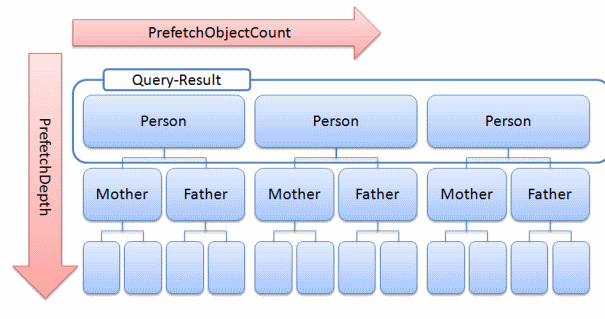
\includegraphics[width=\maxwidth]{images/ref-configuration-client-prefetch-visualisation.png}
\end{center}
\subsection{Prefetch Object Count}
\label{ref:configuration-client-prefetch-object-count}

In a client server scenario, network latency is one of the biggest performance concerns. Instead of making lots of little requests, it's more to do bulk operations. A good way is to prefetch objects which are maybe required later.

The prefect count configures how many objects of a query-result are loaded from the server. Prefetched objects avoid additional roundtrip's to the server for getting the data. However more data needs to be sent to the clients.

\begin{lstlisting}
ClientConfiguration configuration = Db4oClientServer.newClientConfiguration();
configuration.prefetchObjectCount(500);
\end{lstlisting}

{\small\itshape ClientConfigurationExamples.java: Configure the prefetch object count\par}
\medskip

The \hyperref[ref:configuration-client-prefetch-depth]{prefetch depth} (p.~\pageref{ref:configuration-client-prefetch-depth}) and the \hyperref[ref:configuration-client-prefetch-object-count]{prefetch object count} (p.~\pageref{ref:configuration-client-prefetch-object-count}) are closely related to each other. The prefetch object count configures how many objects are prefetched from a query-result. The prefetch-depth configures how deep the object-graph is fetched.

\begin{center}
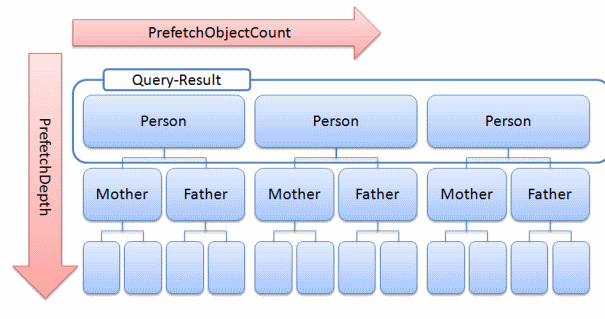
\includegraphics[width=\maxwidth]{images/ref-configuration-client-prefetch-visualisation.png}
\end{center}
\subsection{Prefetch Slot Cache Size}
\label{ref:configuration-client-prefetch-slot-cache-size}

Configures how big the cache for prefetched data is. A larger cache can improve performance, but consumes more memory.

\begin{lstlisting}
ClientConfiguration configuration = Db4oClientServer.newClientConfiguration();
configuration.prefetchSlotCacheSize(1024);
\end{lstlisting}

{\small\itshape ClientConfigurationExamples.java: Configure the slot cache\par}
\medskip

\subsection{Prefetching IDs For New Objects}
\label{ref:configuration-client-prefecht-id-count}

Sets the number of IDs to be pre-allocated new objects created on the client. This avoids requests to allocate new ids when new objects are stored on a client.

When a new object is created on a client, the client should contact the server to get the next available object ID. PrefetchIDCount allows to specify how many IDs should be pre-allocated on the server and prefetched by the client. This method helps to reduce client-server communication.

PrefetchIDCount can be tuned to approximately match the usual amount of objects created in one operation to improve the performance.

When the PrefetchIDCount is one, the client will have to connect to the server for each new objects created. On the other hand,, when the PrefetchIDCount is bigger than the amount of new objects the database will keep unnecessary preallocated ids.

The default PrefetchIDCount is 10.

\subsection{Timeout Client Socket}
\label{ref:configuration-client-timeout-client-socket}

Configure how long it takes, before an inactive connection is timed out.

\begin{lstlisting}
ClientConfiguration configuration = Db4oClientServer.newClientConfiguration();
configuration.timeoutClientSocket(1*60*1000);
\end{lstlisting}

{\small\itshape ClientConfigurationExamples.java: Configure the timeout\par}
\medskip

\section{Networking Configuration}
\label{ref:configuration-network-configuration}

The networking-configuration apply to the client- and the server-mode of db4o. All the networking configuration is accessible via the networking-getter on the configuration-object.

Note that the networking configuration should be the same on the server and all clients.

\subsection*{Overview}

Here's a overview over all networking configuration-settings which you can change:

{\small
\begin{longtable}{|p{\dimexpr(\linewidth-2\arrayrulewidth)*1/1-2\tabcolsep\relax}|}
\hline
\textbf{\hyperref[ref:configuration-networking-batch-mode]{BatchMessages} (p.~\pageref{ref:configuration-networking-batch-mode})}: Enable/Disable batch messages. \\ \hline
\textbf{\hyperref[ref:client-server-messaging]{MessageRecipient} (p.~\pageref{ref:client-server-messaging})}: Set the message receiver. \\ \hline
\textbf{\hyperref[ref:configuration-networking-client-server-factory]{ClientServerFactory} (p.~\pageref{ref:configuration-networking-client-server-factory})}: Replace the client-server factory. \\ \hline
\textbf{\hyperref[ref:configuration-networking-max-batch-queue-size]{MaxBatchQueueSize} (p.~\pageref{ref:configuration-networking-max-batch-queue-size})}: Set the maximum size of the batch queue. \\ \hline
\textbf{\hyperref[ref:configuration-networking-single-threaded-client]{SingleThreadedClient} (p.~\pageref{ref:configuration-networking-single-threaded-client})}: Set the client to single threaded. \\ \hline
\textbf{\hyperref[ref:configuration-networking-pluggable-sockets]{SocketFactory} (p.~\pageref{ref:configuration-networking-pluggable-sockets})}: Set the socket-factory. \\ \hline
\end{longtable}}

\subsection{Batch Mode}
\label{ref:configuration-networking-batch-mode}

Batch mode allows to increase the performance by reducing client/server communication. It's activated by default.

\begin{lstlisting}
ClientConfiguration configuration = Db4oClientServer.newClientConfiguration();
configuration.networking().batchMessages(true);
\end{lstlisting}

{\small\itshape NetworkConfigurationExample.java: enable or disable batch mode\par}
\medskip

db4o communicates with the server by means of messaging. Without batch mode db4o sends a message for each operation and waits for the response. This might be quite inefficient when there are many small messages to be sent (like bulk inserts, updates, deletes). The network communication becomes a bottleneck. Batch messaging mode solves this problem by caching the messages and sending them only when required.

\subsubsection*{Advantages}

\begin{itemize}
\item Reduced network load.
\item Increased performance for bulk operations.
\end{itemize}

\subsubsection*{Disadvantages}

\begin{itemize}
\item Increased memory consumption on both the client and the server. \hyperref[ref:configuration-networking-max-batch-queue-size]{See "Max Batch Queue Size"} (p.~\pageref{ref:configuration-networking-max-batch-queue-size})
\end{itemize}

\subsection{Client Server Factory}
\label{ref:configuration-networking-client-server-factory}

Allows you to change the behavior how a client or a server is created.

This setting should be set to the same value on the server and the clients.

\begin{lstlisting}
ClientConfiguration configuration = Db4oClientServer.newClientConfiguration();
configuration.networking().clientServerFactory(new StandardClientServerFactory());
\end{lstlisting}

{\small\itshape NetworkConfigurationExample.java: exchange the way a client or server is created\par}
\medskip

\subsection{Message Recipient}
\label{ref:configuration-networking-message-recipient}

Register a message recipient for the this object container / server. \hyperref[ref:client-server-messaging]{See "Messaging"} (p.~\pageref{ref:client-server-messaging})

\subsection{Max Batch Queue Size}
\label{ref:configuration-networking-max-batch-queue-size}

To avoid unnecessary network traffic, the client and server can queue up operations, which don't need to be executed immediately. As soon as a message need to be send, all queued messages are send as well. You can configure the maximum of this message queue.

A larger size allows to queue up more messages and avoid unnecessary network roundtrip's. However queued up messages consume additional memory.

\begin{lstlisting}
ClientConfiguration configuration = Db4oClientServer.newClientConfiguration();
configuration.networking().maxBatchQueueSize(1024);
\end{lstlisting}

{\small\itshape NetworkConfigurationExample.java: change the maximum batch queue size\par}
\medskip

\subsection{Single Threaded Client}
\label{ref:configuration-networking-single-threaded-client}

You can configure the client to be single-threaded. When you enable this option, the client doesn't use background threads to handle the client-server communication.

\begin{lstlisting}
ClientConfiguration configuration = Db4oClientServer.newClientConfiguration();
configuration.networking().singleThreadedClient(true);
\end{lstlisting}

{\small\itshape NetworkConfigurationExample.java: single threaded client\par}
\medskip

\subsubsection*{Advantage}

On some smaller embedded systems reducing the running threads improves the performance significantly.

\subsubsection*{Disadvantage}

Since all operations run in a single thread, the operations may take longer. Additionally you cannot receive \hyperref[ref:client-server-messaging]{messages} (p.~\pageref{ref:client-server-messaging}) and cannot use \hyperref[ref:advanced-topics-callbacks-event-registry-api]{commit-callbacks} (p.~\pageref{ref:advanced-topics-callbacks-event-registry-api}) on a single-threaded client.

\subsection{Pluggable Sockets}
\label{ref:configuration-networking-pluggable-sockets}

db4o allows to customize client-server communication by using pluggable socket implementations.

\begin{lstlisting}
ClientConfiguration configuration = Db4oClientServer.newClientConfiguration();
configuration.networking().socketFactory(new StandardSocket4Factory());
\end{lstlisting}

{\small\itshape NetworkConfigurationExample.java: Exchange the socket-factory\par}
\medskip

One use case for changing the socket-implementation is encryption. In fact, db4o's SSL-support uses this mechanism: \hyperref[ref:client-server-pluggable-sockets-using-ssl-for-client-server-communication]{See "Using SSL For Client-Server Communication"} (p.~\pageref{ref:client-server-pluggable-sockets-using-ssl-for-client-server-communication})

\section{Class Specific Configuration}
\label{ref:configuration-objectclass-configuration}

Some settings are object-specific and are configured for the class. It's part of the \hyperref[ref:configuration-common-configuration]{common} (p.~\pageref{ref:configuration-common-configuration})-configuration, which is available on the \hyperref[ref:configuration-client-configuration]{client} (p.~\pageref{ref:configuration-client-configuration}), \hyperref[ref:configuration-server-configuration]{server} (p.~\pageref{ref:configuration-server-configuration}) and \hyperref[ref:configuration]{embedded} (p.~\pageref{ref:configuration})-mode of db4o.

Its recommended that you use the same configuration for the client and the server.

\subsection*{Access the Class Configuration}

The configuration for a specific class follows always the same pattern. First you specify for which type the configuration applies. You pass the type, the name as string or event an instance of the specific class to the configuration.

From the class-configuration, you also can go a level deeper to \hyperref[ref:configuration-objectfield-configuration]{the field configuration} (p.~\pageref{ref:configuration-objectfield-configuration}).

\subsection*{Overview}

Here's a overview over all common configuration-settings which you can change:

{\small
\begin{longtable}{|p{\dimexpr(\linewidth-2\arrayrulewidth)*1/1-2\tabcolsep\relax}|}
\hline
\textbf{\hyperref[ref:configuration-objectclass-call-constructor]{CallConstructor} (p.~\pageref{ref:configuration-objectclass-call-constructor})}: Configure db4o to call constructors when instantiating objects. \\ \hline
\textbf{\hyperref[ref:configuration-objectclass-cascade-on-delete]{CascadeOnDelete} (p.~\pageref{ref:configuration-objectclass-cascade-on-delete})}: When a object is deleted, delete also referenced objects. \\ \hline
\textbf{\hyperref[ref:configuration-objectclass-cascade-on-update]{CascadeOnUpdate} (p.~\pageref{ref:configuration-objectclass-cascade-on-update})}: When a object is updated, update also referenced objects. \\ \hline
\textbf{\hyperref[ref:configuration-objectclass-cascade-on-activate]{CascadeOnActivation} (p.~\pageref{ref:configuration-objectclass-cascade-on-activate})}: When a object is activated, activate also referenced objects. \\ \hline
\textbf{\hyperref[ref:configuration-objectclass-diable-class-index]{Index} (p.~\pageref{ref:configuration-objectclass-diable-class-index})}: Don't index the objects of this type. \\ \hline
\textbf{\sout{EnableReplication}}: Deprecated. \hyperref[ref:configuration-file-generate-uuids]{Generate uuids} (p.~\pageref{ref:configuration-file-generate-uuids}) and \hyperref[ref:configuration-file-generate-timestamps]{commit timestamps} (p.~\pageref{ref:configuration-file-generate-timestamps}) to enable replication. \\ \hline
\textbf{\hyperref[ref:configuration-objectclass-generate-uuid]{GenerateUUIDs} (p.~\pageref{ref:configuration-objectclass-generate-uuid})}: Generate UUIDs, mainly used for replication. \\ \hline
\textbf{\sout{GenerateVersionNumbers}}: Deprecated. Generate \hyperref[ref:configuration-file-generate-timestamps]{commit timestamps} (p.~\pageref{ref:configuration-file-generate-timestamps}) instead. \\ \hline
\textbf{\hyperref[ref:configuration-objectclass-maximum-activation-depth]{MaximumActivationDepth} (p.~\pageref{ref:configuration-objectclass-maximum-activation-depth})}: Set a maximum activation-depth. \\ \hline
\textbf{\hyperref[ref:configuration-objectclass-minimum-activation-depth]{MinimumActivationDeph} (p.~\pageref{ref:configuration-objectclass-minimum-activation-depth})}: Set a minimum activation-depth. \\ \hline
\textbf{\hyperref[ref:configuration-objectclass-persist-static-fields]{PersistStaticFields} (p.~\pageref{ref:configuration-objectclass-persist-static-fields})}: Persist also the static fields of this type. \\ \hline
\textbf{\hyperref[ref:configuration-objectclass-rename-class]{Rename} (p.~\pageref{ref:configuration-objectclass-rename-class})}: Rename this type. Used for \hyperref[ref:advanced-topics-refactoring-and-schema-evolution]{refactorings} (p.~\pageref{ref:advanced-topics-refactoring-and-schema-evolution}). \\ \hline
\textbf{\hyperref[ref:configuration-objectclass-set-a-translator]{Translate} (p.~\pageref{ref:configuration-objectclass-set-a-translator})}: Set a translator for this type. \\ \hline
\textbf{\hyperref[ref:configuration-objectclass-store-transient-fields]{StoreTransientFields} (p.~\pageref{ref:configuration-objectclass-store-transient-fields})}: Store also transient fields. \\ \hline
\textbf{\hyperref[ref:configuration-objectclass-update-depth]{UpdateDepth} (p.~\pageref{ref:configuration-objectclass-update-depth})}: Set the update-depth for this type. \\ \hline
\end{longtable}}

\subsection{Call Constructor}
\label{ref:configuration-objectclass-call-constructor}

By default db4o bypassed the constructor when it loads the objects from the database. When you're class relies on the constructor to be called, for example to initialize transient state, you can enable it. You can do this also on the global configuration for all types. \hyperref[ref:configuration-common-calling-constructors]{See "Calling Constructors"} (p.~\pageref{ref:configuration-common-calling-constructors})

\begin{lstlisting}
EmbeddedConfiguration configuration = Db4oEmbedded.newConfiguration();
configuration.common().objectClass(Person.class).callConstructor(true);
\end{lstlisting}

{\small\itshape ObjectConfigurationExamples.java: Call constructor\par}
\medskip

\subsection{Cascade on Delete}
\label{ref:configuration-objectclass-cascade-on-delete}

When turned on the deletion cascades to all referred objects.

\begin{lstlisting}
EmbeddedConfiguration configuration = Db4oEmbedded.newConfiguration();
configuration.common().objectClass(Person.class).cascadeOnDelete(true);
\end{lstlisting}

{\small\itshape ObjectConfigurationExamples.java: When deleted, delete also all references\par}
\medskip

\subsection{Cascade on Update}
\label{ref:configuration-objectclass-cascade-on-update}

When turned on, the update cascades to all referred objects.

Note: As soon as you use \hyperref[ref:basics-transparent-persistence]{transparent persistence} (p.~\pageref{ref:basics-transparent-persistence}) this configuration option has no effect and isn't needed.

\begin{lstlisting}
EmbeddedConfiguration configuration = Db4oEmbedded.newConfiguration();
configuration.common().objectClass(Person.class).cascadeOnUpdate(true);
\end{lstlisting}

{\small\itshape ObjectConfigurationExamples.java: When updated, update also all references\par}
\medskip

\subsection{Cascade on Activate}
\label{ref:configuration-objectclass-cascade-on-activate}

db4o uses the concept of \hyperref[ref:basics-activation]{activation} (p.~\pageref{ref:basics-activation}) to avoid loading to much data into memory. When turned on the activation cascades for this types. This means that when an instance is activated, all referenced objects are also activated.

Note: As soon as you use \hyperref[ref:basics-transparent-persistence]{transparent activation/persistence} (p.~\pageref{ref:basics-transparent-persistence}) this configuration option has no effect.

\begin{lstlisting}
EmbeddedConfiguration configuration = Db4oEmbedded.newConfiguration();
configuration.common().objectClass(Person.class).cascadeOnActivate(true);
\end{lstlisting}

{\small\itshape ObjectConfigurationExamples.java: When activated, activate also all references\par}
\medskip

\subsection{Disable Class Index}
\label{ref:configuration-objectclass-diable-class-index}

By default there's a index which indexes all instances of a certain type. When you never query this type and only access it by navigation, you can safely disable this index.

\begin{lstlisting}
EmbeddedConfiguration configuration = Db4oEmbedded.newConfiguration();
configuration.common().objectClass(Person.class).indexed(false);
\end{lstlisting}

{\small\itshape ObjectConfigurationExamples.java: Disable class index\par}
\medskip

\subsection{Generate UUIDs}
\label{ref:configuration-objectclass-generate-uuid}

Generate UUIDs for instances of this type. UUIDs are mainly used for \hyperref[drs:welcome]{replication} (p.~\pageref{drs:welcome}).

\begin{lstlisting}
EmbeddedConfiguration configuration = Db4oEmbedded.newConfiguration();
configuration.common().objectClass(Person.class).generateUUIDs(true);
\end{lstlisting}

{\small\itshape ObjectConfigurationExamples.java: Generate uuids for this type\par}
\medskip

\subsection{Maximum Activation Depth}
\label{ref:configuration-objectclass-maximum-activation-depth}

Sets the maximum \hyperref[ref:basics-activation]{activation depth} (p.~\pageref{ref:basics-activation}) for this type. Useful to avoid accidentally activating large objects.

Note: As soon as you use \hyperref[ref:basics-transparent-persistence]{transparent activation/persistence} (p.~\pageref{ref:basics-transparent-persistence}) this configuration option has no effect.

\begin{lstlisting}
EmbeddedConfiguration configuration = Db4oEmbedded.newConfiguration();
configuration.common().objectClass(Person.class).maximumActivationDepth(5);
\end{lstlisting}

{\small\itshape ObjectConfigurationExamples.java: Set maximum activation depth\par}
\medskip

\subsection{Minimum Activation Depth}
\label{ref:configuration-objectclass-minimum-activation-depth}

Sets the minimum \hyperref[ref:basics-activation]{activation depth} (p.~\pageref{ref:basics-activation}) for this type. Useful to load always load referenced objects.

Note: As soon as you use \hyperref[ref:basics-transparent-persistence]{transparent activation/persistence} (p.~\pageref{ref:basics-transparent-persistence}) this configuration option has no effect.

\begin{lstlisting}
EmbeddedConfiguration configuration = Db4oEmbedded.newConfiguration();
configuration.common().objectClass(Person.class).minimumActivationDepth(2);
\end{lstlisting}

{\small\itshape ObjectConfigurationExamples.java: Set minimum activation depth\par}
\medskip

\subsection{Persist Static Fields}
\label{ref:configuration-objectclass-persist-static-fields}

By default db4o doesn't store static fields. With this setting you force db4o to also store the value of the static fields. Note that only reference types are stored. Value-types like ints, longs etc are not persisted.

In general you shouldn't store static fields, because this can lead to unexpected behaviors. It's mostly useful for enumeration classes. \hyperref[ref:advanced-topics-type-handling-static-fields-and-enums-static-fields-api]{See "Storing Static Fields"} (p.~\pageref{ref:advanced-topics-type-handling-static-fields-and-enums-static-fields-api})

\begin{lstlisting}
EmbeddedConfiguration configuration = Db4oEmbedded.newConfiguration();
configuration.common().objectClass(Person.class).persistStaticFieldValues();
\end{lstlisting}

{\small\itshape ObjectConfigurationExamples.java: Persist also the static fields\par}
\medskip

\subsection{Rename Class}
\label{ref:configuration-objectclass-rename-class}

You can rename a class. Useful when you reactor you're code. \hyperref[ref:advanced-topics-refactoring-and-schema-evolution]{See "Refactoring and Schema Evolution"} (p.~\pageref{ref:advanced-topics-refactoring-and-schema-evolution})

\begin{lstlisting}
EmbeddedConfiguration configuration = Db4oEmbedded.newConfiguration();
configuration.common().objectClass(Person.class).rename("com.db4odoc.new.package.NewName");
\end{lstlisting}

{\small\itshape ObjectConfigurationExamples.java: Rename this type\par}
\medskip

\subsection{Set a Translator}
\label{ref:configuration-objectclass-set-a-translator}

You can specify a special translator for this type. A translator is a special way to add you're custom serialization for a type. \hyperref[ref:advanced-topics-type-handling-translators]{See "Translators"} (p.~\pageref{ref:advanced-topics-type-handling-translators})

\begin{lstlisting}
EmbeddedConfiguration configuration = Db4oEmbedded.newConfiguration();
configuration.common().objectClass(Person.class).translate(new TSerializable());
\end{lstlisting}

{\small\itshape ObjectConfigurationExamples.java: Use a translator for this type\par}
\medskip

\subsection{Store Transient Fields}
\label{ref:configuration-objectclass-store-transient-fields}

By default db4o doesn't store transient fields. With this setting you can force db4o to event store transient fields.

\begin{lstlisting}
EmbeddedConfiguration configuration = Db4oEmbedded.newConfiguration();
configuration.common().objectClass(Person.class).storeTransientFields(true);
\end{lstlisting}

{\small\itshape ObjectConfigurationExamples.java: Store also transient fields\par}
\medskip

\subsection{Update Depth}
\label{ref:configuration-objectclass-update-depth}

By default db4o only stores changes on the updated object, but not the changes on referenced objects. With a higher update-depth db4o will traverse along the object graph to a certain depth and update all objects. \hyperref[ref:basics-update-concept]{See "Update Concept"} (p.~\pageref{ref:basics-update-concept}). You can also specify this \hyperref[ref:configuration-common-update-depth]{globally} (p.~\pageref{ref:configuration-common-update-depth}).

\begin{lstlisting}
EmbeddedConfiguration configuration = Db4oEmbedded.newConfiguration();
configuration.common().objectClass(Person.class).updateDepth(2);
\end{lstlisting}

{\small\itshape ObjectConfigurationExamples.java: Set the update depth\par}
\medskip

\section{Field Specific Configuration}
\label{ref:configuration-objectfield-configuration}

Some settings are field-specific. It's part of the \hyperref[ref:configuration-objectclass-configuration]{object} (p.~\pageref{ref:configuration-objectclass-configuration})-configuration, which is available on the client, server and embedded-mode of db4o.

Its recommended that you use the same configuration for the client and the server.

\subsection*{Access the Field Configuration}

The configuration for a field follows the same pattern. First you specify for which type this configuration applies. You pass the type or the name as string. Then you navigate to the specific field by passing the field name as string.

\subsection{Adding a Field Index}
\label{ref:configuration-objectfield-configuration:adding}

Index dramatically speed up queries. You should index all fields which you run queries on. \hyperref[ref:basics-indexing]{See "Indexing"} (p.~\pageref{ref:basics-indexing})

\begin{lstlisting}
@Indexed
private String zipCode;
\end{lstlisting}

{\small\itshape City.java: Index a field\par}
\medskip

As alternative you can externally configure a field index:

\begin{lstlisting}
EmbeddedConfiguration configuration = Db4oEmbedded.newConfiguration();
configuration.common().objectClass(Person.class).objectField("name").indexed(true);
\end{lstlisting}

{\small\itshape ObjectFieldConfigurations.java: Index a certain field\par}
\medskip

As an alternative you also can use the appropriate Annotation on the field which you want to index.

\subsection{Cascade On Activate}
\label{ref:configuration-objectfield-configuration:cascadeactivate}

db4o uses the concept of \hyperref[ref:basics-activation]{activation} (p.~\pageref{ref:basics-activation}) to avoid loading to much data into memory. When this setting is turned on, the object referenced by this field is activated, when the object is activated.

Note: As soon as you use \hyperref[ref:basics-transparent-persistence]{transparent activation/persistence} (p.~\pageref{ref:basics-transparent-persistence}) this configuration option has no effect.

\begin{lstlisting}
EmbeddedConfiguration configuration = Db4oEmbedded.newConfiguration();
configuration.common().objectClass(Person.class).objectField("father").cascadeOnActivate(true);
\end{lstlisting}

{\small\itshape ObjectFieldConfigurations.java: When activated, activate also the object referenced by this field\par}
\medskip

\subsection{Cascade On Update}
\label{ref:configuration-objectfield-configuration:cascadeupdate}

When the object is updated, the object referenced by this field is also updated.

Note: As soon as you use \hyperref[ref:basics-transparent-persistence]{transparent persistence} (p.~\pageref{ref:basics-transparent-persistence}) this configuration option has no effect and isn't needed.

\begin{lstlisting}
EmbeddedConfiguration configuration = Db4oEmbedded.newConfiguration();
configuration.common().objectClass(Person.class).objectField("father").cascadeOnUpdate(true);
\end{lstlisting}

{\small\itshape ObjectFieldConfigurations.java: When updated, update also the object referenced by this field\par}
\medskip

\subsection{Cascade On Delete}
\label{ref:configuration-objectfield-configuration:cascadedelete}

When the object is deleted, the object referenced by this field is also deleted

\begin{lstlisting}
EmbeddedConfiguration configuration = Db4oEmbedded.newConfiguration();
configuration.common().objectClass(Person.class).objectField("father").cascadeOnDelete(true);
\end{lstlisting}

{\small\itshape ObjectFieldConfigurations.java: When deleted, delete also the object referenced by this field\par}
\medskip

\subsection{Rename Field}
\label{ref:configuration-objectfield-configuration:rename}

Allows you to rename this field. . \hyperref[ref:advanced-topics-refactoring-and-schema-evolution]{See "Refactoring and Schema Evolution"} (p.~\pageref{ref:advanced-topics-refactoring-and-schema-evolution})

\begin{lstlisting}
EmbeddedConfiguration configuration = Db4oEmbedded.newConfiguration();
configuration.common().objectClass(Person.class).objectField("name").rename("sirname");
\end{lstlisting}

{\small\itshape ObjectFieldConfigurations.java: Rename this field\par}
\medskip

\section{Id System}
\label{ref:configuration-id-system}

The id-system configuration applies to the embedded- and the server-mode of db4o. There are tree different id-systems-available. All the id system configuration is accessible via the id-system-getter on the configuration-object.

Note that you cannot change the id-system for an existing database. You need to \hyperref[ref:advanced-topics-defragment]{defragment} (p.~\pageref{ref:advanced-topics-defragment}) the database in order to change the id-system.

The id-system is responsible to mapping a object id to the physical location of an object. This mapping can have significant impact on the performance.

\subsection*{Stacked BTree Id-System}

This setting uses a stack of two BTree's on top of an InMemoryIdSystem. This system is scalable for a large number of ids.

\begin{lstlisting}
EmbeddedConfiguration configuration = Db4oEmbedded.newConfiguration();
configuration.idSystem().useStackedBTreeSystem();
\end{lstlisting}

{\small\itshape IdSystemConfigurationExamples.java: Use stacked B-trees for storing the ids\par}
\medskip

\subsection*{Single BTree Id-System}

This setting uses a single BTree on top of a in memory id system. This system works great for small databases. However it cannot scale for a large number of ids.

\begin{lstlisting}
EmbeddedConfiguration configuration = Db4oEmbedded.newConfiguration();
configuration.idSystem().useSingleBTreeSystem();
\end{lstlisting}

{\small\itshape IdSystemConfigurationExamples.java: Use a single B-tree for storing the ids.\par}
\medskip

\subsection*{In Memory Id-System}

This id-system keeps all ids in memory. While accessing the ids if fast, all ids have to be written to disk on every commit. Therefore it can be used only for tiny databases.

\begin{lstlisting}
EmbeddedConfiguration configuration = Db4oEmbedded.newConfiguration();
configuration.idSystem().useInMemorySystem();
\end{lstlisting}

{\small\itshape IdSystemConfigurationExamples.java: Use a in-memory id system\par}
\medskip

\subsection*{Pointer Based Id-System}

This id system uses pointers to handle ids. Each id represents a pointer into the database-file. This makes the id-mapping simple. However since it's a pointer, you cannot change the location. Therefore this system leads to more fragmentation and performance degradation as the database grows.

This id system is here to ensure backward-compatibility. It's not recommended to use for new databases.

\begin{lstlisting}
EmbeddedConfiguration configuration = Db4oEmbedded.newConfiguration();
configuration.idSystem().usePointerBasedSystem();
\end{lstlisting}

{\small\itshape IdSystemConfigurationExamples.java: Use pointers for storing the ids\par}
\medskip

\subsection*{Custom Id-System}

It's possible to implement your own id system. You can pass an factory which creates your id-system implementation.

\begin{lstlisting}
EmbeddedConfiguration configuration = Db4oEmbedded.newConfiguration();
configuration.idSystem().useCustomSystem(new CustomIdSystemFactory());
\end{lstlisting}

{\small\itshape IdSystemConfigurationExamples.java: use a custom id system\par}
\medskip

\section{Server Configuration}
\label{ref:configuration-server-configuration}

The server-configuration applies to the \hyperref[ref:client-server]{db4o-server} (p.~\pageref{ref:client-server}). All the server specific configuration is directly on the client configuration interface.

You can also configure the \hyperref[ref:configuration-common-configuration]{common} (p.~\pageref{ref:configuration-common-configuration})-, \hyperref[ref:configuration-file-configuration]{file} (p.~\pageref{ref:configuration-file-configuration})-, \hyperref[ref:configuration-id-system]{id-system} (p.~\pageref{ref:configuration-id-system})- and the \hyperref[ref:configuration-network-configuration]{network} (p.~\pageref{ref:configuration-network-configuration})-settings for a server.

\subsection*{Server Socket Timeout}

Configure how long it takes, before an inactive connection is timed out.

\begin{lstlisting}
ServerConfiguration configuration = Db4oClientServer.newServerConfiguration();
configuration.timeoutServerSocket(10*60*1000);
\end{lstlisting}

{\small\itshape ServerConfigurationExamples.java: configure the socket-timeout\par}
\medskip


% Converted from reference/DB4OFlare (MadCap Flare, Java target)

\chapter{Client-Server}
\label{ref:client-server}

db4o's is an embedded database which usually runs in process. Nevertheless db4o also supports a client server setup. There's no ready to use db4o server, instead you embedded the db4o server in a regular application. This gives you full how you want to run the db4o server.

In order to use the db4o client server mode you need to include the db4o-X.XX-cs-javaC.jar if your not using the db4o-X.XX-all-javaX.jar in your project. \hyperref[ref:dependency-overview]{See "Dependency Overview"} (p.~\pageref{ref:dependency-overview})

\section*{Start The Server}

You start the server by creating a object server instance with the client server factory. Pass the database file path and the port to the factory. After that you need to specify a user-name and password which clients can use to login to this server. You can add multiple users by calling the grant access method multiple times.

\begin{lstlisting}
ObjectServer server = Db4oClientServer.openServer("database.db4o",8080);
try{
    server.grantAccess("user","password");

    // Let the server run.
    letServerRun();
} finally {
    server.close();
}
\end{lstlisting}

{\small\itshape ServerExample.java: Start a db4o server\par}
\medskip

\section*{Connect To The Server}

After the server is up an running you can connect to it. Pass the URL, port, user name and password to the client server factory. This will return a client object container. After that the container is ready to use.

\begin{lstlisting}
final ObjectContainer container
        = Db4oClientServer.openClient("localhost", 8080, "user", "password");
try{
    // Your operations
}finally {
    container.close();
}
\end{lstlisting}

{\small\itshape Db4oClientExample.java: Connect to the server\par}
\medskip

\section*{Client-Server Setup}

When using a client server setup you should check following things:

\begin{itemize}
\item Ensure that the client and server use the same db4o version.
\item Both, the server and client should have access to classes of the stored objects. When the classes differ between the client and server or are missing unspecified behavior can occur.
\end{itemize}

\section{Reference Cache In Client-Server Mode}
\label{ref:client-server-reference-cache-in-client-server-mode}

db4o uses an \hyperref[ref:basics-indentity-concept-reference-cache]{object reference cache} (p.~\pageref{ref:basics-indentity-concept-reference-cache}) for easy access to persistent objects during one transaction. In client/server mode each client has its own reference cache, which helps to achieve good performance. However it gets complicated, when different clients work on the same object, as this object's cached value is used on each side. It means, that even when the operations go serially, the object's value won't be updated serially unless it is refreshed before each update.

\begin{lstlisting}
Person personOnClient1 = queryForPerson(client1);
Person personOnClient2 = queryForPerson(client2);
System.out.println(queryForPerson(client2).getName());

personOnClient1.setName("New Name");
client1.store(personOnClient1);
client1.commit();

// The other client still has the old data in the cache
System.out.println(queryForPerson(client2).getName());

client2.ext().refresh(personOnClient2,Integer.MAX_VALUE);

// After refreshing the date is visible
System.out.println(queryForPerson(client2).getName());
\end{lstlisting}

{\small\itshape ReferenceCacheExamples.java: Reference cache in client server\par}
\medskip

There are multiple strategies to deal with this.

\begin{itemize}
\item If you client's are not updating the same object or it very unlikely that it happens, you don't need to take any action.
\item You can refresh objects as they are updated on all clients. However this need a lot of communication between the server and client. \hyperref[ref:client-server-refreshing-objects]{See "Refreshing Objects"} (p.~\pageref{ref:client-server-refreshing-objects})
\item You can do short unit of work on the client, to minimize the chance of outdated objects.
\end{itemize}

\subsection*{Clean Cache For Work}

Often you don't want to refresh object by object. Instead you want to work with a clean cache. You can do this by using a separate 'session' on the client. This container brings its own cache with it. So you can create a new container which a clean cache.

Note that open session on the client doesn't create a separate transaction. Instead it only creates a fresh cache. The transaction is always the same.

\begin{lstlisting}
ObjectContainer container = client.ext().openSession();
try{
    // do work
}finally {
    container.close();
}
// Start with a fresh cache:
container = client.ext().openSession();
try{
    // do work
}finally {
    container.close();
}
\end{lstlisting}

{\small\itshape ReferenceCacheExamples.java: Clean cache for each unit of work\par}
\medskip

\subsection{Refreshing Objects}
\label{ref:client-server-refreshing-objects}

When working with multiple client object-containers each container has its own reference cache. When you query for objects, you get always the cached objects. This means, that objects probably have been updated in the mean-time but the client still sees the old state.

For some scenarios you might need to refresh to objects to bring it up to date. There are two strategies for this. You can explicit refresh a object at any time. Or you can use callbacks to refresh object on each commit. Both methods have their advantage.

{\small
\begin{longtable}{|p{\dimexpr(\linewidth-4\arrayrulewidth)*1/3-2\tabcolsep\relax}|p{\dimexpr(\linewidth-4\arrayrulewidth)*1/3-2\tabcolsep\relax}|p{\dimexpr(\linewidth-4\arrayrulewidth)*1/3-2\tabcolsep\relax}|}
\hline
 & Explicit Refreshing & Using Callbacks \\ \hline
Advantage & \begin{itemize}
\item Selective refreshing possible, which reduces network traffic.
\item Can decide when a refresh is required. If no refresh is required, you can save the network traffic.
\end{itemize} & \begin{itemize}
\item The objects are always up to date.
\item There's no need to explicitly refresh-calls in your data-access layer.
\end{itemize} \\ \hline
Disadvantage & \begin{itemize}
\item Partial refreshed objects may lead to a inconsistent object-graph.
\item Probably a lot of refresh-calls spread over the code-base.
\end{itemize} & \begin{itemize}
\item A lot of network traffic is required to send the committing-events and object to the clients.
\end{itemize} \\ \hline
\end{longtable}}

\subsubsection*{Explicitly Refreshing Objects}

You can refresh objects with the refresh-method on the object-container. The pass the object to refresh and the refresh-depth to the method:

\begin{lstlisting}
db.ext().refresh(objToRefresh,Integer.MAX_VALUE);
\end{lstlisting}

{\small\itshape RefreshingObjects.java: refresh a object\par}
\medskip

\subsubsection*{Using Callbacks For Refreshing Objects}

You can use the committed-event to refresh objects as soon as another client commits. Take a look at the example: \hyperref[ref:advanced-topics-callbacks-possible-usecases-committed-event-example]{See "Committed Event Example"} (p.~\pageref{ref:advanced-topics-callbacks-possible-usecases-committed-event-example})

\section{Embedded Clients}
\label{ref:client-server-embedded}

db4o supports embedded containers or session container. It's a separate object-container with its own transaction and own reference cache. \hyperref[ref:advanced-topics-session-containers]{See "Session Containers"} (p.~\pageref{ref:advanced-topics-session-containers})

Now if you're using the client-server mode for db4o, you also can create such sessions directly from the server. When you pass a 0 to the open server method, the server only supports embedded clients. With any other port you can connect with \hyperref[ref:client-server]{regular clients} (p.~\pageref{ref:client-server}) and also create embedded clients.

\begin{lstlisting}
ObjectServer server = Db4oClientServer.openServer(DATABASE_FILE_NAME, 0);

// open the db4o-embedded client. For example at the beginning for a web-request
ObjectContainer container = server.openClient();
try {
    // do the operations on the session-container
    container.store(new Person("Joe"));
} finally {
    // close the container. For example when the request ends
    container.close();
}
\end{lstlisting}

{\small\itshape Db4oSessions.java: Embedded client\par}
\medskip

\subsection*{OpenSession On A Client}

You might noted that the open-session is available on any object-container. Normally this creates a \hyperref[ref:advanced-topics-session-containers]{session-container} (p.~\pageref{ref:advanced-topics-session-containers}) with its own transaction and reference cache. However on a db4o-client this is not true. There it only creates a container with new cache, but shares the transaction with the client. The only use case for this is to implement connection pooling.\hyperref[ref:client-server-pooling]{See "Client-Container Pooling"} (p.~\pageref{ref:client-server-pooling})

\section{Native Queries}
\label{ref:client-server-native-queries}

Native Queries are optimized to SODA under the hood. Therefore they can be normally used in a client-server environment. However, there is a catch: as soon as the native query is not optimized there will be two things required on the server:

\begin{itemize}
\item The persistent classes definitions will be required because the objects will need to be instantiated to execute the query code.
\item The native predicate class will be required to run on the server to do the actual job.
\end{itemize}

To meet these requirements you can keep your persistent classes and NQ predicates in separate libraries, which will make it easy to deploy it on both the client and the server side. Otherwise you may try to express the unoptimised query in \hyperref[ref:basics-querying-soda-query]{SODA} (p.~\pageref{ref:basics-querying-soda-query}), this option will make it more performant, but the disadvantage is less robust and maintainable code.

\section{Anonymous Classes In Client Server Mode}
\label{ref:client-server-anonymous-classes}

Anonymous classes are used to implement Native Query predicates, Comparators and Evaluations. In this case it is important to remember that in client/server mode they will be marshaled and sent together with the graph of referenced objects to the server. The catch here is that anonymous classes contain a reference to their parent class, meaning that the parent class will be marshalled as well!

This has two issues:

\begin{itemize}
\item All the stuff referenced by the parent class will be marshaled and sent too. This means additional traffic between the server and the client.
\item The parent class maybe contains stuff which cannot be serialized.
\item You can only use anonymous classes when the client and the server have all classes available refered by the anonymous class. This means in fact that the server should have the same classes available as the client.
\end{itemize}

Note that when a native query can be optimized, the anonymous class isn't used, but rather \hyperref[ref:basics-querying-soda-query]{SODA} (p.~\pageref{ref:basics-querying-soda-query}). In such cases this issues don't apply.

\section{Server Without Persistent Classes Deployed}
\label{ref:client-server-server-without-persistent-classes-deployed}

We recommend to ensure that the client and server have classes of the stored objects available. So you need to include the classes of the stored object in the server process.

Running the server without classes is can cause unexpected behavior and should only be used when you are up to experiments.

When classes are unknown GenericReflector creates generic objects, which hold simulated "field values" in an array of objects. This is done automatically by db4o engine and does not require any additional settings from your side: you can save, retrieve and modify objects just as usual. An example of this functionality is db4o's \hyperref[ref:object-manager-enterprise]{Object Manager} (p.~\pageref{ref:object-manager-enterprise}).

Unfortunately in a server without persistent classes mode there are still some limitations:

\begin{itemize}
\item Evaluation queries won't work. This also implies that native queries which cannot be optimized don't work.
\item Native queries will only work if they can be optimized
\item Multidimensional arrays can not be stored.
\end{itemize}

\subsection*{Native Queries}

Native queries are \hyperref[ref:basics-querying-native-queries-native-query-optimization]{usually translated to SODA} (p.~\pageref{ref:basics-querying-native-queries-native-query-optimization}) queries. When a native query can be translated to SODA, it will run fine on a server without persisted classes. However when the query cannot be optimized the server needs the native query instance and the data model which isn't available on a server without persistent classes. Therefore native queries only work when it can be optimized. You can fallback to pure \hyperref[ref:basics-querying-soda-query]{SODA queries} (p.~\pageref{ref:basics-querying-soda-query}) in such cases.

\section{Events In Client Server-Mode}
\label{ref:client-server-events-in-cs-mode}

Events of course also work in client server mode. This topic only applies to the networked client/server mode. Embedded client/server-mode isn't affected. There the events work the same way as in the embedded-mode. \hyperref[ref:advanced-topics-callbacks-event-registry-api]{See "Event Registry API"} (p.~\pageref{ref:advanced-topics-callbacks-event-registry-api})

\subsection*{Separate Event Registry For Each Client}

Each client has its own event registry. When you register to a event on the client-event-registry, events will be fired for actions on the client. You won't receive events for actions on other clients.

Furthermore you cannot register for the delete-events, the delete events is only on the server available.

\subsection*{The Server Event Registry}

The server has its own event registry. When you register to an event on the server registry, events will be fired for all action of the clients and the server itself. So you can monitor all operations on the server.

Note that in some events the server isn't involved. For example when a client activates some object, the server is no involved, an therefore no event is fired on the server.

Use central server object container to register for the events on the server.

\begin{lstlisting}
ObjectServer server = 
        Db4oClientServer.openServer(DATABASE_FILE_NAME, PORT_NUMBER);
EventRegistry eventsOnServer =
        EventRegistryFactory.forObjectContainer(server.ext().objectContainer());
\end{lstlisting}

{\small\itshape EventRegistryExamples.java: register for events on the server\par}
\medskip

\subsection*{Committed Event On All Parties}

The committed event is an exception. When a client or the server commits, every client and the server will fire the committed event. This way a client can inform itself that another client has made changes to the database.

However this involves communication overhead to send the message to all the clients. Therefore you should use this event only when absolutely necessary on the clients.

\subsection*{Events Are Fired Asynchronous}

In client-server-mode the events are fired asynchronous. This means that you event-handler is invoked in a separate thread. You need to ensure that you lock any shared data-structure you access from the event-handlers.

\section{Client-Container Pooling}
\label{ref:client-server-pooling}

When a client connects to the server, there's overhead to establish the connection. First the regular TCP-connection needs to be established. Then the server and client exchange meta data and finally the connection is ready. If you don't need a single or a few long during connections but rather short units of work on the client it is quite inefficient to open a client connection for each unit of work. In such scenarios you should consider to pool the client-containers.

Now simply pooling the raw client container might lead to issues. Each object-container has a \hyperref[ref:basics-indentity-concept-reference-cache]{reference-cache} (p.~\pageref{ref:basics-indentity-concept-reference-cache}). When you pool the object-container and reuse it for some other work, this cache isn't cleared. This means that you might get dirty objects from the reference cache. You want to avoid this and have a clean cache when reusing the client container.

There's a way to archive that. On the client container the open session method creates a fresh object container with a clean reference cache which is sharing the transaction with the client. With this building block you can build a proper container pool.

First you need to create client connections on demand which will be pooled.

\begin{lstlisting}
ObjectContainer client = Db4oClientServer.openClient("localhost",PORT,
                USER_AND_PASSWORD, USER_AND_PASSWORD);
\end{lstlisting}

{\small\itshape ConnectionPoolExamples.java: Open clients for the pool\par}
\medskip

On a request for a object container, get a client container from the pool. Rollback the transaction on it to ensure that it is in a clean state.Then open a session container on it and use this session. The session-container ensures that the reference-cache is empty. Make sure that each client container is always used only once at any time, which means that there's always only one session-container open per client-container. The session-containers share the transaction with the client and you don't want to share transactions across multiple object containers.

\begin{lstlisting}
// Obtain a client container. Either take one from the pool or allocate a new one
ObjectContainer client = obtainClientContainer();
// Make sure that the transaction is in clean state
client.rollback();
// Then create a session on that client container and use it for the database operations.
// The client-container is now in use. Ensure that it isn't leased twice.
final ObjectContainer sessionContainer = client.ext().openSession();
\end{lstlisting}

{\small\itshape ConnectionPool.java: Obtain a pooled container\par}
\medskip

Now when you're done with your operations, you can return the client to your pool of object containers. First close the session-container, which commits the changes and releases the resources. Then get the underlying client-container for that session and return it to the pool.

\begin{lstlisting}
// First you need to get the underlying client for the session
final ObjectContainer client = clientForSession(session);
// then the client is ready for reuse
returnToThePool(client);
\end{lstlisting}

{\small\itshape ConnectionPool.java: Returning to pool\par}
\medskip

\section{Concurrency Control}
\label{ref:client-server-concurrency-control}

As soon as you will start using db4o with multiple client connections you will recognize the necessity of implementing a concurrency control system. db4o itself works as an overly optimistic scheme, i.e. an object is locked for read and write, but no collision check is made. This approach makes db4o very flexible and gives you an opportunity to organize a concurrency control system, which will suit your needs the best. Your main tools to build your concurrency control system would be:

\begin{itemize}
\item \hyperref[ref:client-server-semaphores]{Semaphores} (p.~\pageref{ref:client-server-semaphores})
\item \hyperref[ref:advanced-topics-callbacks]{Callbacks} (p.~\pageref{ref:advanced-topics-callbacks})
\end{itemize}

The articles in this topic set will show you how to implement locking and will give you an advice which strategy to use in different situations.

\subsection{Semaphores}
\label{ref:client-server-semaphores}

db4o semaphores are named flags that can only be owned by one object container at one time. They are supplied to be used as locks for exclusive access to code blocks in applications and to signal states from one client to the server and to all other clients.

The naming of semaphores is up to the application. Any string can be used.

Semaphores are freed automatically when a client disconnects correctly or when a clients presence is no longer detected by the server, that constantly monitors all client connections.

\begin{lstlisting}
// Grab the lock. Specify the name and a timeout in milliseconds
boolean hasLock = container.ext().setSemaphore("LockName", 1000);
try {
    // you need to check the lock
    if (hasLock) {
        System.out.println("Could get lock");
    } else{
        System.out.println("Couldn't get lock");
    }
} finally {
    // release the lock
    container.ext().releaseSemaphore("LockName");
}
\end{lstlisting}

{\small\itshape SemaphoreExamples.java: Grab a semaphore\par}
\medskip

\subsubsection*{Building Block}

Semaphores are a low level building block. Usually they are not used directly. Instead you can build the abstractions you need with semaphores. For example you can build object-locking, critical sections etc with semaphores.

\section{Messaging}
\label{ref:client-server-messaging}

In client/server it possible to send messages between a client and the server. Possible use cases could be:

\begin{itemize}
\item Shutting down and restarting the server.
\item Triggering server backup.
\item Using a customized login strategy to restrict the number of allowed client connections.
\item Running special code on the server. For example batch updates.
\end{itemize}

\subsection*{Sending and Receiving Messages}

First you need to decide on a class that you want to use as the message. Any object that is storable in db4o can be used as a message. Of course you use multiple classes for representing different messages. Let's create a dedicated class.

\begin{lstlisting}
public class HelloMessage {
    private final String message;

    public HelloMessage(String message) {
        this.message = message;
    }

    @Override
    public String toString() {
        return message;
    }
}
\end{lstlisting}

{\small\itshape HelloMessage.java: The message class\par}
\medskip

Now you need to register a handler to handle arriving messages. This can be done by configuring a message recipient on the server. Let's simply print out the arriving message. Additionally we answer to the client with another message.

\begin{lstlisting}
ServerConfiguration configuration = Db4oClientServer.newServerConfiguration();
configuration.networking().messageRecipient(new MessageRecipient() {
    public void processMessage(MessageContext messageContext, Object o) {
        System.out.println("The server received a '" + o + "' message");
        // you can respond to the client
        messageContext.sender().send(new HelloMessage("Hi Client!"));
    }
});
ObjectServer server = Db4oClientServer.openServer(configuration, DATABASE_FILE, PORT_NUMBER);
\end{lstlisting}

{\small\itshape MessagingExample.java: configure a message receiver for the server\par}
\medskip

The same can be done on the client. Register a handler for the received messages.

\begin{lstlisting}
ClientConfiguration configuration = Db4oClientServer.newClientConfiguration();
configuration.networking().messageRecipient(new MessageRecipient() {
    public void processMessage(MessageContext messageContext, Object o) {
        System.out.println("The client received a '" + o + "' message");
    }
});
\end{lstlisting}

{\small\itshape MessagingExample.java: configure a message receiver for a client\par}
\medskip

Now on the client we can get a message sender. The message sender allows you to send a message to the server. In this example we send a hello message.

\begin{lstlisting}
MessageSender sender = configuration.messageSender();
ObjectContainer container = Db4oClientServer.openClient(configuration, "localhost", PORT_NUMBER, USER_AND_PASSWORD, USER_AND_PASSWORD);

sender.send(new HelloMessage("Hi Server!"));
\end{lstlisting}

{\small\itshape MessagingExample.java: Get the message sender and use it\par}
\medskip

\section{Using SSL For Client-Server Communication}
\label{ref:client-server-pluggable-sockets-using-ssl-for-client-server-communication}

With the default settings db4o client-server communication is not encrypted and thus can potentially be a dangerous security hole. db4o supports SSL for client server communication. The implementation uses the \hyperref[ref:configuration-networking-pluggable-sockets]{pluggable socket} (p.~\pageref{ref:configuration-networking-pluggable-sockets}) to provide secure sockets.

The SSL-communication uses the standard Java Secure Socket Extensions, which are part of the normal JRE. You take a look a to \href{http://java.sun.com/javase/technologies/security/}{full documentation here}.

You simply need to add the SSLSupport on the server and the clients and you done. The default-implementation uses the default SSLContext for the client and the server.

\begin{lstlisting}
ServerConfiguration configuration = Db4oClientServer.newServerConfiguration();
configuration.common().add(new SSLSupport());
\end{lstlisting}

{\small\itshape SSLExample.java: Add SSL-support to the server\par}
\medskip

\begin{lstlisting}
ClientConfiguration configuration = Db4oClientServer.newClientConfiguration();
configuration.common().add(new SSLSupport());
\end{lstlisting}

{\small\itshape SSLExample.java: Add SSL-support to the client\par}
\medskip

Of course you also can build your own SSLContext with the Java API. After you've build the SSL-Context, you can pass it to the SSLSupport-constructor. Read in the Java documentation how to \href{http://java.sun.com/javase/6/docs/technotes/guides/security/jsse/JSSERefGuide.html}{build a proper SSLContext:}

\begin{lstlisting}
// You can build your own SSLContext and use all features of Java's SSL-support.
// To keep this example small, we just use the default-context instead of building one.
SSLContext context = SSLContext.getDefault();

ServerConfiguration configuration = Db4oClientServer.newServerConfiguration();
configuration.common().add(new SSLSupport(context));
\end{lstlisting}

{\small\itshape SSLExample.java: You can build up a regular SSL-Context and us it\par}
\medskip

\section{Client-Server Timeouts}
\label{ref:client-server-client-server-timeouts}

Every client/server application has to face a problem of network communications. Luckily modern protocols screen the end-application from all fixable problems. However there are still physical reasons that can't be fixed by a protocol: disconnections, power failures, crash of a system on the other end of communication channel etc. In these cases it is still the responsibility of the client-server application to exit the connection gracefully, releasing all resources and protecting data.

In order to achieve an efficient client/server communication and handling of connection problems the following requirements were defined for db4o:

\begin{itemize}
\item The connection should not be terminated when both client and server are still alive, even if either of the machines is running under heavy load.
\item Whenever a client dies, peacefully or with a crash, the server should clean up all resources that were reserved for the client.
\item Whenever a server goes offline, it should be possible for the client to detect that there is a problem.
\item Since many clients may be connected at the same time, it makes sense to be careful with the resources the server reserves for each client.
\item A client can be a very small machine, so it would be good if the client application can work with a single thread.
\end{itemize}

The current approach tries to keep things as simple as possible: any connection is closed immediately upon a timeout. In order to prevent closing connections when there is no communication between client and server due to reasons different from connection problems a separate timer thread was created to send messages to the server at a regular basis. The server must reply to the thread immediately, if this does not happen the communication channel gets closed.

This approach works effectively for both client and server side. However there's are small downside to this. When a server operation takes longer than the timeout, the connection will be closed. You can configure the timeouts for the \hyperref[ref:configuration-client-timeout-client-socket]{client} (p.~\pageref{ref:configuration-client-timeout-client-socket}) and the \hyperref[ref:configuration-server-configuration]{server} (p.~\pageref{ref:configuration-server-configuration}).

An easy rule of thumb:

\begin{itemize}
\item If you experience clients disconnecting, raise the timeout value.
\item If you have a system where clients crash frequently or where the network is very instable, lower the values, so resources for disconnected clients are freed faster.
\end{itemize}


% Converted from reference/DB4OFlare (MadCap Flare, Java target)

\chapter{Best Practices}
\label{ref:best-practises}

This topic is a collection of best practices for db4o.

db4o doesn't have any support for limiting the result size or skipping objects in the result set. You can do this on top of db4o with little effort. \hyperref[ref:best-practises-paging]{See "Paging"} (p.~\pageref{ref:best-practises-paging})

How should you scope the lifetime of an object container? See this guide-line: \hyperref[ref:best-practises-lifetime-of-a-objectcontainer]{See "Lifetime Of On Object Container"} (p.~\pageref{ref:best-practises-lifetime-of-a-objectcontainer})

Deleting object is always a delicate process. \hyperref[ref:best-practises-deleting-objects]{See "Deleting Objects"} (p.~\pageref{ref:best-practises-deleting-objects})

If you upgrade to new major db4o version you should do these steps to update the file format. \hyperref[ref:best-practises-updating-db4o-version]{See "Upgrade db4o Version"} (p.~\pageref{ref:best-practises-updating-db4o-version})

\section{Managing Relations}
\label{ref:best-practises-managing-relations}

In db4o you manage relations by storing references to other objects. In db4o navigational access is usually a lot faster than queries. Therefore think about how you navigate to the right information. This topic gives an overview how to manage different relations.

\subsection{1-N Relation: Navigating from 1 to N}
\label{ref:best-practises-managing-relations:1ton-nav}

As example we use shopping cards which hold items. In most use cases you need to know which items are on a card. For that you navigate from the card (the 1-part) to the items (the N-part). In this case you simply can use a collection on the shopping card which references all items.

Keep in mind that a \hyperref[ref:basics-querying-soda-soda-performance-characteristics]{contains-query on collections is very slow} (p.~\pageref{ref:basics-querying-soda-soda-performance-characteristics}). Finding out which items are on a certain shopping cards is very slow. If you want to know that, take a look at the suggestions below.

\begin{lstlisting}
Set<Item> items = new HashSet<Item>();

public void add(Item terrain) {
    items.add(terrain);
}

public void remove(Item o) {
    items.remove(o);
}
\end{lstlisting}

{\small\itshape ShoppingCard.java: Simple 1-n relation. Navigating from the card to the items\par}
\medskip

\subsection{1-N Relation: Navigating from N to 1}
\label{ref:best-practises-managing-relations:nto1-nav}

Imagine that you store people and in which country a person is born. Here you usually navigate from the person (the N-part) to the country (the 1-part). Therefore you can have a field which refers to the country.

In the rare case where you want to know all people born in a certain country you can do a query. When the country reference is \hyperref[ref:basics-indexing]{indexed} (p.~\pageref{ref:basics-indexing}), then that query is fast.

\begin{lstlisting}
// Optionally we can index this field, when we want to find all people for a certain country
private Country bornIn;

public Country getBornIn() {
    return bornIn;
}
\end{lstlisting}

{\small\itshape Person.java: Simple 1-n relation. Navigating from the person to the countries\par}
\medskip

Getting all people of a country is not that hard and fast when the `bornIn' field is indexed.

\begin{lstlisting}
final Country country = loadCountry(container,"USA");
final ObjectSet<Person> peopleBurnInTheUs = container.query(new Predicate<Person>() {
    @Override
    public boolean match(Person p) {
        return p.getBornIn() == country;
    }
});
\end{lstlisting}

{\small\itshape RelationManagementExamples.java: Query for people burn in a country\par}
\medskip

\subsection{1-N Relation: Bidirectional}
\label{ref:best-practises-managing-relations:1ton-bidirect}

When you want to navigate a 1-N relationship bidirectional you can use the method above, because the query if fast enough. Just ensure that you index the field holding the reference.

Alternatively you also can add an additional collection which holds the items. However in that case you need to manually manage the consistency of the relation.

For example the relationship between dogs and their owners. The dog has a field with its owner, while the person has a collection of his dogs. The setters then manage the relationship and ensure that it is always consistent.

\begin{lstlisting}
private Person owner;

// This setter ensures that the model is always consistent
public void setOwner(Person owner) {
    if(null!=this.owner){
        Person oldOwner = this.owner;
        this.owner = null;
        oldOwner.removeOwnerShipOf(this);
    }
    if(null!=owner && !owner.ownedDogs().contains(this)) {
        owner.addOwnerShipOf(this);
    }
    this.owner = owner;
}

public Person getOwner() {
    return owner;
}
\end{lstlisting}

{\small\itshape Dog.java: Bidirectional 1-N relations. The dog has a owner\par}
\medskip

\begin{lstlisting}
private Set<Dog> owns = new HashSet<Dog>();

// The add and remove method ensure that the relations is always consistent
public void addOwnerShipOf(Dog dog) {
    owns.add(dog);
    dog.setOwner(this);
}

public void removeOwnerShipOf(Dog dog) {
    owns.remove(dog);
    dog.setOwner(null);
}

public Collection<Dog> ownedDogs() {
    return Collections.unmodifiableCollection(owns);
}
\end{lstlisting}

{\small\itshape Person.java: Bidirectional 1-N relations. The person has dogs\par}
\medskip

\subsection{N-N Relations: One Way Navigation}
\label{ref:best-practises-managing-relations:nton-nav}

Like 1-N relations N-N relations also can be one directional. For example a person can have multiple citizenships in different countries. Let's suppose that you only want to know the citizenship of a person and not the citizens of a country. Then you navigate from people to countries. You can store that in a simple collection.

Keep in mind that a \hyperref[ref:basics-querying-soda-soda-performance-characteristics]{contains-query on a collection is very slow} (p.~\pageref{ref:basics-querying-soda-soda-performance-characteristics}). Finding the people of a certain country will be very slow.

\begin{lstlisting}
private Set<Country> citizenIn = new HashSet<Country>();

public void removeCitizenship(Country o) {
    citizenIn.remove(o);
}

public void addCitizenship(Country country) {
    citizenIn.add(country);
}
\end{lstlisting}

{\small\itshape Person.java: One directional N-N relation\par}
\medskip

\subsection{N-N Relations: Bidirectional Navigation}
\label{ref:best-practises-managing-relations:nton-bidirect}

For managing bidirectional N-N relations you can use collections, but maintain a collection on both sides. For example a club has a member-list and each member has a list of clubs where he is a member.

Keep in mind that a \hyperref[ref:basics-querying-soda-soda-performance-characteristics]{contains-query on a collection is very slow} (p.~\pageref{ref:basics-querying-soda-soda-performance-characteristics}). That's why you maintain two collections, so that you can navigate to the club-members or club-membership.

\begin{lstlisting}
private Set<Person> members = new HashSet<Person>();

public void addMember(Person person) {
    if (!members.contains(person)) {
        members.add(person);
        person.join(this);
    }
}

public void removeMember(Person person) {
    if (members.contains(person)) {
        members.remove(person);
        person.leave(this);
    }
}
\end{lstlisting}

{\small\itshape Club.java: Bidirectional N-N relation\par}
\medskip

\begin{lstlisting}
private Set<Club> memberIn = new HashSet<Club>();

public void join(Club club) {
    if (!memberIn.contains(club)) {
        memberIn.add(club);
        club.addMember(this);
    }
}

public void leave(Club club) {
    if (memberIn.contains(club)) {
        memberIn.remove(club);
        club.removeMember(this);
    }
}

public Collection<Club> memberOf() {
    return Collections.unmodifiableCollection(memberIn);
}
\end{lstlisting}

{\small\itshape Person.java: Bidirectional N-N relation\par}
\medskip

\section{Paging}
\label{ref:best-practises-paging}

Currently db4o doesn't provide any paging mechanism at all. However all db4o query results are lazy loaded. db4o returns a result list which only contains the ids of the objects and will load the object as soon as you access it. This means you can page by only accessing the indexes of the range you're interested in.

Since the result sets of db4o implement the Java List interface it has the sub list method. With this method you easily get only a sub set of the result. Or you can build your own paging-method based on the sub list method on the lists.

\begin{lstlisting}
public static <T> List<T> paging(List<T> listToPage, int limit){
    return paging(listToPage,0,limit);
}

public static <T> List<T> paging(List<T> listToPage, int start, int limit){
    if(start>listToPage.size()){
        throw new IllegalArgumentException("You cannot start the paging outside the list." +
                " List-size: "+listToPage.size()+" start: "+start);
    }
    int end = calculateEnd(listToPage, start, limit);
    return listToPage.subList(start, end);

}

private static <T> int calculateEnd(List<T> resultList, int start, int limit) {
    int end = start + limit;
    if(end>=resultList.size()){
        return resultList.size();
    }
    return end;
}
\end{lstlisting}

{\small\itshape PagingUtility.java: Paging utility methods\par}
\medskip

And then of course you can use the utility methods on the result-sets of db4o.

\begin{lstlisting}
final ObjectSet<StoredItems> queryResult = container.query(StoredItems.class);
List<StoredItems> pagedResult = PagingUtility.paging(queryResult, 2, 2);
\end{lstlisting}

{\small\itshape TestPagingUtility.java: Use the paging utility\par}
\medskip

\section{Upgrade db4o Version}
\label{ref:best-practises-updating-db4o-version}

How do you upgrade to a newer version safely? By default db4o can read an older version of a database and operate on it without any issues. However for major version updates you should consider doing this updating procedure. This ensures that the database uses the newest file format and performance optimizations.

\subsection*{The safest update procedure:}

\begin{enumerate}
\item \hyperref[ref:advanced-topics-defragment]{Defragment} (p.~\pageref{ref:advanced-topics-defragment}) the database with the current version. This will automatically also create a backup.
\item Upgrade to the new db4o version.
\item After that immediately \hyperref[ref:advanced-topics-defragment]{defragment} (p.~\pageref{ref:advanced-topics-defragment}) the database with the current version. This will create another backup. After that the database file uses the most current database format.
\item Make sure that you can read the data from the database. If everything works you can delete the backups.
\end{enumerate}

\section{Lifetime Of An Object Container}
\label{ref:best-practises-lifetime-of-a-objectcontainer}

The main interface to your database is the \hyperref[ref:basics-object-container]{object container} (p.~\pageref{ref:basics-object-container}). You do all major operations with a object container instance. Now how long should you keep a object container open? Is it better to close the object container after each operation. Or keep the object container open? This topic is a small guideline on the lifetime of an object container.

\subsection*{Understanding Object Containers}

The lifetime of a object container heavily depends on your application scenario. Therefore it's vital to understand what a object container represents. A object container consist of a \hyperref[ref:basics-acid-and-transactions]{transaction} (p.~\pageref{ref:basics-acid-and-transactions}) and a \hyperref[ref:basics-indentity-concept-reference-cache]{reference} (p.~\pageref{ref:basics-indentity-concept-reference-cache}) cache and is thread safe. This means that a object container is isolated from other containers. Furthermore an object container has a cache, so you don't want to throw a object container away if you don't have to.

\subsection*{One Object Container Per Unit Of Work}

This means in fact that you should use one object container per unit of work. You can use a object container for succeeding units of work. But you should never use the same object container for concurrent or independent units of work. You can create \hyperref[ref:advanced-topics-session-containers]{new object containers at any time} (p.~\pageref{ref:advanced-topics-session-containers}).

\subsection*{Desktop Application}

What does this mean for a desktop application? Well in a simple desktop application you might can use only one object container. Since there only one user doing something at a time you can use the same object container for all operations.

For complexes desktop application multiple object container can be an option. For example a object container per tab, per wizard etc.

Be aware only because object container is thread safe it doesn't make your object model thread safe. If multiple threads are using the same object container they will use the same objects and modify the same object concurrently. You need to use an appropriate model for the concurrent access.

\subsection*{Web Application}

In a web application you should use a \hyperref[ref:platform-specific-issues-web-web-isolation]{object container per request} (p.~\pageref{ref:platform-specific-issues-web-web-isolation}). Each request is it unit of work. Maybe there are multiple unit of work successively in a request, but a request represents the top level unit of work.

\section{Deleting Objects}
\label{ref:best-practises-deleting-objects}

Deleting object is always a delicate process. Deleting the wrong object can be catastrophic. Here are some best practices for deleting objects.

\subsection*{Delete Flag}

When a end user deletes a object it's often better to use a deleted-flag instead of actually deleting the data. This has the advantage that you can undo the delete operation at any time. Also you don't break the model in cases where the user deleted the wrong object. However it has also some disadvantages. You need to honor the deleted-flag in your queries.

You can set the delete flag in a \hyperref[ref:advanced-topics-callbacks]{callback} (p.~\pageref{ref:advanced-topics-callbacks}) and use the regular db4o delete operation:

\begin{lstlisting}
EventRegistry events = EventRegistryFactory.forObjectContainer(container);
events.deleting().addListener(new EventListener4<CancellableObjectEventArgs>() {
    public void onEvent(Event4<CancellableObjectEventArgs> events,
                        CancellableObjectEventArgs eventArgument) {
        Object obj = eventArgument.object();
        // if the object has a deletion-flag:
        // set the flag instead of deleting the object
        if (obj instanceof Deletable) {
            ((Deletable) obj).delete();
            eventArgument.objectContainer().store(obj);
            eventArgument.cancel();
        }
    }
});
\end{lstlisting}

{\small\itshape DeletionStrategies.java: Deletion-Flag\par}
\medskip

However you need to filter the deleted objects in every query.

\subsection*{Be Very Careful}

db4o doesn't support any referential integrity. When you delete a object and there's still a reference to that object this reference is set to null. This means if you delete a object you may break the consistency of you're object model.

This means also that you need to implement any consistency check yourself on top of db4o. You can use db4o \hyperref[ref:advanced-topics-callbacks]{callbacks} (p.~\pageref{ref:advanced-topics-callbacks}) for doing so.

\subsection*{Use Cascade Deletion Wisely}

You can configure db4o the cascade delete referenced objects. You can configure that for \hyperref[ref:configuration-objectclass-cascade-on-delete]{certain type} (p.~\pageref{ref:configuration-objectclass-cascade-on-delete}) or \hyperref[ref:configuration-objectfield-configuration]{certain fields} (p.~\pageref{ref:configuration-objectfield-configuration}). As said there's no referential integrity checks for db4o, so you have to extreamly conscious where to use this feature. It makes sense to configure cascade deletion for composition roots, where you are sure that the children cannot be referenced from another location. In all other places it's a bad idea most of the time.


% Converted from reference/DB4OFlare (MadCap Flare, Java target)

\chapter{Platform Specific Issues}
\label{ref:platform-specific-issues}

Db4o can be run in a variety of environments, which have Java virtual machine or .NET CLR. We use a common core code base, which allows automatic production of db4o builds for the following platforms:

\begin{itemize}
\item Java JDK 5 or newer
\item .NET 3.5 or newer
\item .NET 3.5 CompactFramework
\item Mono (you need to compile db4o yourself)
\item Android
\item Silverlight
\end{itemize}

Db4o has a small database footprint and requires minimum processing resources thus being an excellent choice for embedded use in smartphones, photocopiers, car electronics, and packaged software (including real-time monitoring systems). It also shows good performance and reliability in web and desktop applications.

You can use db4o on desktop with:

\begin{itemize}
\item Windows (Java, .Net)
\item Linux (Java, Mono).
\end{itemize}

On mobile and embedded devices with:

\begin{itemize}
\item Android
\item Windows CE or Windows Mobile (.NET Compact Framework)
\end{itemize}

db4o provides the same API for all platforms, however each platform has its own features, which should be taken into consideration in software development process. These features will be discussed in the following chapters.

More Reading:

\begin{itemize}
\item \hyperref[ref:platform-specific-issues-db4o-on-java-platforms]{db4o on Java Platforms} (p.~\pageref{ref:platform-specific-issues-db4o-on-java-platforms})
\item \hyperref[ref:platform-specific-issues-security-requirements-on-java-platform]{Security Requirements On Java Platform} (p.~\pageref{ref:platform-specific-issues-security-requirements-on-java-platform})
\item \hyperref[ref:platform-specific-issues-web-servlets]{Servlets} (p.~\pageref{ref:platform-specific-issues-web-servlets})
\item \hyperref[ref:platform-specific-issues-database-for-osgi]{Database For OSGi} (p.~\pageref{ref:platform-specific-issues-database-for-osgi})
\item \hyperref[ref:platform-specific-issues-android]{Android} (p.~\pageref{ref:platform-specific-issues-android})
\end{itemize}

\section{Disconnected Objects}
\label{ref:platform-specific-issues-disconnected-objects}

db4o manages objects \hyperref[ref:basics-identity-concept]{by object-identity} (p.~\pageref{ref:basics-identity-concept}). db4o ensures that each stored object in the database is always represented by the same object in memory. When you load an object, change it and then store it, db4o recognizes the object by its identity and will update it.

This model works wonderful as long as the object-identity is preserved. However there are a lot of scenarios, where the object-identity is lost. As soon as serialize objects, the object-identity is lost. This is typical for web-scenarios or web-services, where a object needs to be identified across requests. For such scenarios objects need additional ids to identify object across requests- and object-container-boundaries.

There are several possibilities for such additional ids. You can use db4o internal ids, \hyperref[ref:advanced-topics-ids-and-uuids]{db4o uuids} (p.~\pageref{ref:advanced-topics-ids-and-uuids}), or additional ids-fields on objects. Each has its advantages and disadvantages, so take a looks at this comparison: \hyperref[ref:platform-specific-issues-disconnected-objects-comparison-of-ids]{See "Comparison Of Different IDs"} (p.~\pageref{ref:platform-specific-issues-disconnected-objects-comparison-of-ids})

Only identifying the object across object container boundaries is often not enough. You actually need to update a disconnected object. This is done by coping the new values to the existing object. \hyperref[ref:platform-specific-issues-disconnected-objects-merging-changes]{See "Merging Changes"} (p.~\pageref{ref:platform-specific-issues-disconnected-objects-merging-changes})

\subsection{Comparison Of Different IDs}
\label{ref:platform-specific-issues-disconnected-objects-comparison-of-ids}

There are a lot of possibilities for additional ids to identify objects across the object container boundary.

\subsubsection*{Internal db4o ids}

db4o has internal ids to identify each object in the database. You can access these ids and use them yourself. . Take a look at the example. \hyperref[ref:platform-specific-issues-disconnected-objects-example-internal-id]{See "Example Internal Id"} (p.~\pageref{ref:platform-specific-issues-disconnected-objects-example-internal-id})

{\small
\begin{longtable}{|p{\dimexpr(\linewidth-3\arrayrulewidth)*1/2-2\tabcolsep\relax}|p{\dimexpr(\linewidth-3\arrayrulewidth)*1/2-2\tabcolsep\relax}|}
\hline
\textbf{Advantages} & \textbf{Disadvantages} \\ \hline
\begin{itemize}
\item Internal ids are fast.
\item No additional field on the class required.
\item No additional configuration required.
\end{itemize} & \begin{itemize}
\item The id may change when defragmentating the database.
\end{itemize} \\ \hline
\end{longtable}}

\subsubsection*{db4o UUIDs}

db4o supports special UUIDs. You can enable them by configuration. . Take a look at the example. \hyperref[ref:platform-specific-issues-disconnected-objects-example-db4o-uuid]{See "Example db4o UUID"} (p.~\pageref{ref:platform-specific-issues-disconnected-objects-example-db4o-uuid})

{\small
\begin{longtable}{|p{\dimexpr(\linewidth-3\arrayrulewidth)*1/2-2\tabcolsep\relax}|p{\dimexpr(\linewidth-3\arrayrulewidth)*1/2-2\tabcolsep\relax}|}
\hline
\textbf{Advantages} & \textbf{Disadvantages} \\ \hline
\begin{itemize}
\item A UUID is a worldwide unique id.
\item No additional field on the class required.
\end{itemize} & \begin{itemize}
\item db4o UUIDs are large.
\item db4o UUID is db4o-specific type.
\end{itemize} \\ \hline
\end{longtable}}

\subsubsection*{UUID-Fields on Classes}

You can add UUID-fields to your classes. In the constructor of the object you assign a new UUID to the object. Then you can find the object by a regular query. Add \hyperref[ref:advanced-topics-type-handling-uuid-support]{UUID support} (p.~\pageref{ref:advanced-topics-type-handling-uuid-support}) before using UUIDs . Don't forget \hyperref[ref:basics-indexing]{to index the id-field} (p.~\pageref{ref:basics-indexing}). Take a look at the example. \hyperref[ref:platform-specific-issues-disconnected-objects-example-plattform-uuid]{See "Example "} (p.~\pageref{ref:platform-specific-issues-disconnected-objects-example-plattform-uuid})

{\small
\begin{longtable}{|p{\dimexpr(\linewidth-3\arrayrulewidth)*1/2-2\tabcolsep\relax}|p{\dimexpr(\linewidth-3\arrayrulewidth)*1/2-2\tabcolsep\relax}|}
\hline
\textbf{Advantages} & \textbf{Disadvantages} \\ \hline
\begin{itemize}
\item A UUID is a worldwide unique id .
\item UUID are easy to generate and portable.
\end{itemize} & \begin{itemize}
\item You need an id-field on your objects.
\item UUIDs are quite large.
\item Additional index required.
\end{itemize} \\ \hline
\end{longtable}}

\subsubsection*{ID-Field On Classes With a ID-Generator}

You can add a id-field to your classes and then use an ID-Generator to assign new ids to stored objects. Don't forget \hyperref[ref:basics-indexing]{to index the id-field} (p.~\pageref{ref:basics-indexing}). Take a look at the example. \hyperref[ref:platform-specific-issues-disconnected-objects-example-id-generator]{See "Example ID-Generator"} (p.~\pageref{ref:platform-specific-issues-disconnected-objects-example-id-generator})

{\small
\begin{longtable}{|p{\dimexpr(\linewidth-3\arrayrulewidth)*1/2-2\tabcolsep\relax}|p{\dimexpr(\linewidth-3\arrayrulewidth)*1/2-2\tabcolsep\relax}|}
\hline
\textbf{Advantages} & \textbf{Disadvantages} \\ \hline
\begin{itemize}
\item A simple id on objects.
\item Familiar model from the RDBMS-world.
\end{itemize} & \begin{itemize}
\item You need an id-field on your objects.
\item You need to implement an ID-Generator. Which isn't trivial.
\item Additional index required.
\end{itemize} \\ \hline
\end{longtable}}

\subsubsection{Example Internal Id}
\label{ref:platform-specific-issues-disconnected-objects-example-internal-id}

This example demonstrates how you can use internal object ids to identify objects across objects containers. Take a look advantages and disadvantages of internal ids: \hyperref[ref:platform-specific-issues-disconnected-objects-comparison-of-ids]{See "Comparison Of Different IDs"} (p.~\pageref{ref:platform-specific-issues-disconnected-objects-comparison-of-ids})

For using the internal ids no additional configuration is required. You can get this id for any object.

You can get the internal id from the extended object container.

\begin{lstlisting}
long interalId = container.ext().getID(obj);
\end{lstlisting}

{\small\itshape Db4oInternalIdExample.java: get the db4o internal ids\par}
\medskip

Getting a object by its id is also easy. First you get the object from the container. Unlike queries this won't return a \hyperref[ref:basics-activation]{activated} (p.~\pageref{ref:basics-activation}) object. So you have to do it explicitly.

\begin{lstlisting}
long internalId =idForObject;
Object objectForID = container.ext().getByID(internalId);
// getting by id doesn't activate the object
// so you need to do it manually
container.ext().activate(objectForID);
\end{lstlisting}

{\small\itshape Db4oInternalIdExample.java: get an object by db4o internal id\par}
\medskip

\subsubsection{Example db4o UUID}
\label{ref:platform-specific-issues-disconnected-objects-example-db4o-uuid}

This example demonstrates how you can use db4o-UUIDs to identify objects across objects containers. Take a look advantages and disadvantages of db4o-UUIDs: \hyperref[ref:platform-specific-issues-disconnected-objects-comparison-of-ids]{See "Comparison Of Different IDs"} (p.~\pageref{ref:platform-specific-issues-disconnected-objects-comparison-of-ids})

First you need to enable db4o-UUIDs in order to use it.

\begin{lstlisting}
configuration.file().generateUUIDs(ConfigScope.GLOBALLY);
\end{lstlisting}

{\small\itshape Db4oUuidExample.java: db4o-uuids need to be activated\par}
\medskip

With UUIDs turned on, db4o will create an UUID for each stored object. So you can get the UUID of the object from the object-container.

\begin{lstlisting}
Db4oUUID uuid = container.ext().getObjectInfo(obj).getUUID();
\end{lstlisting}

{\small\itshape Db4oUuidExample.java: get the db4o-uuid\par}
\medskip

Getting a object by its UUID is also easy. First you get the object from the container. Unlike queries this won't \hyperref[ref:basics-activation]{activate} (p.~\pageref{ref:basics-activation}) your object. So you have to do it explicitly.

\begin{lstlisting}
Object objectForId = container.ext().getByUUID(idForObject);
// getting by uuid doesn't activate the object
// so you need to do it manually
container.ext().activate(objectForId);
\end{lstlisting}

{\small\itshape Db4oUuidExample.java: get an object by a db4o-uuid\par}
\medskip

\subsubsection{Example UUID}
\label{ref:platform-specific-issues-disconnected-objects-example-plattform-uuid}

This example demonstrates how you can use UUID s to identify objects across objects containers. Take a look advantages and disadvantages of UUID s: \hyperref[ref:platform-specific-issues-disconnected-objects-comparison-of-ids]{See "Comparison Of Different IDs"} (p.~\pageref{ref:platform-specific-issues-disconnected-objects-comparison-of-ids})

Don't forget to add \hyperref[ref:advanced-topics-type-handling-uuid-support]{UUID support} (p.~\pageref{ref:advanced-topics-type-handling-uuid-support}).

This example assumes that all object have a common super class, IDHolder, which holds the UUID in a field.

\begin{lstlisting}
private final UUID uuid = UUID.randomUUID();

public UUID getObjectId(){
    return uuid;
}
\end{lstlisting}

{\small\itshape IDHolder.java: generate the id\par}
\medskip

It's important to index the id-field, otherwise looking up for object by id will be slow.

\begin{lstlisting}
configuration.common().add(new UuidSupport());
configuration.common().objectClass(IDHolder.class).objectField("uuid").indexed(true);
\end{lstlisting}

{\small\itshape UuidOnObject.java: index the uuid-field\par}
\medskip

The id is hold by the object itself, so you can get it directly.

\begin{lstlisting}
IDHolder uuidHolder = (IDHolder)obj;
UUID uuid = uuidHolder.getObjectId();
\end{lstlisting}

{\small\itshape UuidOnObject.java: get the uuid\par}
\medskip

You can get the object you can by a regular query.

\begin{lstlisting}
Query query = container.query();
query.constrain(IDHolder.class);
query.descend("uuid").constrain(idForObject);
IDHolder object= (IDHolder) query.execute().get(0);
\end{lstlisting}

{\small\itshape UuidOnObject.java: get an object its UUID\par}
\medskip

\subsubsection{Example ID-Generator}
\label{ref:platform-specific-issues-disconnected-objects-example-id-generator}

This example demonstrates how you can use an ID-generator to identify objects across objects containers. Take a look advantages and disadvantages of ID-generators: \hyperref[ref:platform-specific-issues-disconnected-objects-comparison-of-ids]{See "Comparison Of Different IDs"} (p.~\pageref{ref:platform-specific-issues-disconnected-objects-comparison-of-ids})

This example assumes that all object have a common super class, IDHolder, which holds the id.

\begin{lstlisting}
private int id;
public int getId() {
    return id;
}

public void setId(int id) {
    this.id = id;
}
\end{lstlisting}

{\small\itshape IDHolder.java: id holder\par}
\medskip

Don't forget to index the id-field. Otherwise finding objects by id will be slow.

\begin{lstlisting}
configuration.common().objectClass(IDHolder.class).objectField("id").indexed(true);
\end{lstlisting}

{\small\itshape AutoIncrementExample.java: index the id-field\par}
\medskip

The hard part is to write an efficient ID-Generator. For this example a very simple \hyperref[ref:advanced-topics-callbacks-possible-usecases-autoincrement]{auto increment generator} (p.~\pageref{ref:advanced-topics-callbacks-possible-usecases-autoincrement}) is used. Use the \hyperref[ref:advanced-topics-callbacks-event-registry-api]{creating-callback-event} (p.~\pageref{ref:advanced-topics-callbacks-event-registry-api}) in order to add the ids to the object. When committing, store the state of the id-generator.

\begin{lstlisting}
final AutoIncrement increment = new AutoIncrement(container);
EventRegistry eventRegistry = EventRegistryFactory.forObjectContainer(container);
eventRegistry.creating().addListener(new EventListener4<CancellableObjectEventArgs>() {
    public void onEvent(Event4<CancellableObjectEventArgs> event4,
                        CancellableObjectEventArgs objectArgs) {
        if(objectArgs.object() instanceof IDHolder){
            IDHolder idHolder = (IDHolder) objectArgs.object();
            idHolder.setId(increment.getNextID(idHolder.getClass()));
        }
    }
});
eventRegistry.committing().addListener(new EventListener4<CommitEventArgs>() {
    public void onEvent(Event4<CommitEventArgs> commitEventArgsEvent4,
                        CommitEventArgs commitEventArgs) {
        increment.storeState();
    }
});
\end{lstlisting}

{\small\itshape AutoIncrementExample.java: use events to assign the ids\par}
\medskip

The id is hold by the object itself, so you can get it directly.

\begin{lstlisting}
IDHolder idHolder = (IDHolder)obj;
int id = idHolder.getId();
\end{lstlisting}

{\small\itshape AutoIncrementExample.java: get the id\par}
\medskip

You can get the object you can by a regular query.

\begin{lstlisting}
Object object = container.query(new Predicate<IDHolder>() {
    @Override
    public boolean match(IDHolder o) {
        return o.getId() == id;
    }
}).get(0);
\end{lstlisting}

{\small\itshape AutoIncrementExample.java: get an object by its id\par}
\medskip

\subsection{Merging Changes}
\label{ref:platform-specific-issues-disconnected-objects-merging-changes}

Merging the changes is the most challenging part when using disconnected objects. Imagine that we have a disconnected object, which contains the changes. We have to store the changes somehow. You cannot simply store the disconnected object, because db4o wouldn't recognize it and store a new object instead of updating the old one. \hyperref[ref:platform-specific-issues-disconnected-objects-wrong-approach]{See "Wrong Approach"} (p.~\pageref{ref:platform-specific-issues-disconnected-objects-wrong-approach})

Instead you need to load the existing object and then copy the state from the disconnected object to the loaded object. Basically you traverse the object-graph and copy all changes over. \hyperref[ref:platform-specific-issues-disconnected-objects-example-merge-changes]{See "Example Merge Changes"} (p.~\pageref{ref:platform-specific-issues-disconnected-objects-example-merge-changes})

db4o has no built-in merge support. However there are external libraries which can help you to merge changes, like  \href{http://dozer.sourceforge.net/}{Dozer}.

\subsubsection{Wrong Approach}
\label{ref:platform-specific-issues-disconnected-objects-wrong-approach}

The wrong approach is to try to store disconnected objects. db4o manages object by their \hyperref[ref:basics-identity-concept]{object-identity} (p.~\pageref{ref:basics-identity-concept}) and doesn't recognize objects which have been serialized or loaded by another object container instance. This example shows, that instead of updating the object, db4o will store a new instance of the object.

\begin{lstlisting}
{
    ObjectContainer container = openDatabase();
    Pilot joe = queryByName(container,"Joe");
    container.close();

    // The update on another object container
    ObjectContainer otherContainer = openDatabase();
    joe.setName("Joe New");
    otherContainer.store(joe);
    otherContainer.close();
}
{
    // instead of updating the existing pilot,
    // a new instance was stored.
    ObjectContainer container = openDatabase();
    ObjectSet<Pilot> pilots = container.query(Pilot.class);
    System.out.println("Amount of pilots: "+pilots.size());
    for (Pilot pilot : pilots) {
        System.out.println(pilot);
    }
    container.close();
}
\end{lstlisting}

{\small\itshape ObjectIdentityExamples.java: Update doesn't works when using the different object containers\par}
\medskip

So in order to update an object, you need to load and store it in the same object-container. If you cannot do this, you need to merge to object-changes. \hyperref[ref:platform-specific-issues-disconnected-objects-example-merge-changes]{See "Example Merge Changes"} (p.~\pageref{ref:platform-specific-issues-disconnected-objects-example-merge-changes})

\begin{lstlisting}
{
    ObjectContainer container = openDatabase();
    Pilot joe = queryByName(container,"Joe");
    joe.setName("Joe New");
    container.store(joe);
    container.close();
}
{
    ObjectContainer container = openDatabase();
    ObjectSet<Pilot> pilots = container.query(Pilot.class);
    System.out.println("Amount of pilots: "+pilots.size());
    for (Pilot pilot : pilots) {
        System.out.println(pilot);
    }
    container.close();
}
\end{lstlisting}

{\small\itshape ObjectIdentityExamples.java: Update works when using the same object container\par}
\medskip

\subsubsection{Example Merge Changes}
\label{ref:platform-specific-issues-disconnected-objects-example-merge-changes}

This example shows how changes are merged from the disconnected object to the object to update. To do this, traverse the object-graph and copy all value types over. All reference types are first checked if they are an existing object. If it is,the primitives are copied over, otherwise it's a stored as a new object.

\begin{lstlisting}
ObjectContainer container = openDatabase();

// first get the object from the database
Car carInDb = getCarById(container,disconnectedCar.getObjectId());

// copy the value-objects (int, long, double, string etc)
carInDb.setName(disconnectedCar.getName());

// traverse into the references
Pilot pilotInDB = carInDb.getPilot();
Pilot disconnectedPilot = disconnectedCar.getPilot();

// check if the object is still the same
if(pilotInDB.getObjectId().equals(disconnectedPilot.getObjectId())){
    // if it is, copy the value-objects
    pilotInDB.setName(disconnectedPilot.getName());
    pilotInDB.setPoints(disconnectedPilot.getPoints());
} else{
    // otherwise replace the object
    carInDb.setPilot(disconnectedPilot); 
}

// finally store the changes
container.store(pilotInDB);
container.store(carInDb);
\end{lstlisting}

{\small\itshape MergeExample.java: merging\par}
\medskip

You can use reflection to automated this process. You can also use existing libraries like  \href{http://dozer.sourceforge.net/}{Dozer} which help you to do this.

\section{Web Environment}
\label{ref:platform-specific-issues-web-environment}

db4o runs perfectly well in a web environment. It can be used to build your web-application.

In most web-application multiple concurrent requests are processes. Normally you want to isolate each request from another. You can use db4o transactions to archive this isolation. \hyperref[ref:platform-specific-issues-web-web-isolation]{See "Isolation in Web-Applications".} (p.~\pageref{ref:platform-specific-issues-web-web-isolation})

In most web-applications a object is only alive during a request. So you have to identify objects across requests. Therefore you need to add an additional id to your object. There are different possibilities for this. \hyperref[ref:platform-specific-issues-disconnected-objects]{See "Disconnected Objects"} (p.~\pageref{ref:platform-specific-issues-disconnected-objects})

When you run in a web-environment, you often have stricter security limitations. Take a look at the security requirements. \hyperref[ref:platform-specific-issues-security-requirements-on-java-platform]{See "Security Requirements"} (p.~\pageref{ref:platform-specific-issues-security-requirements-on-java-platform})

Take a look how you create a object-container for each request. \hyperref[ref:platform-specific-issues-web-servlets]{See "Servlets"} (p.~\pageref{ref:platform-specific-issues-web-servlets})

Take a look at a small example Spring MVC application.\hyperref[ref:platform-specific-issues-web-spring-mvc-example]{See "Spring MVC Example"} (p.~\pageref{ref:platform-specific-issues-web-spring-mvc-example})

\subsection{Isolation in Web-Applications}
\label{ref:platform-specific-issues-web-web-isolation}

In most web-application multiple concurrent request are processes. You want to isolate the request from each other. db4o supports \hyperref[ref:basics-acid-and-transactions]{transactions} (p.~\pageref{ref:basics-acid-and-transactions}), which are perfect for this kind of isolation. Each unit of work gets its own transaction, for example each request. You can create a new session object container for this purpose. Such a session-container brings its own transaction and reference-system. This ensures that the session container is isolated from other operations on the database.

\begin{lstlisting}
ObjectContainer rootContainer = Db4oEmbedded.openFile(DATABASE_FILE_NAME);

// open the db4o-session. For example at the beginning for a web-request
ObjectContainer session = rootContainer.ext().openSession();
try {
    // do the operations on the session-container
    session.store(new Person("Joe"));
} finally {
    // close the container. For example when the request ends
    session.close();
}
\end{lstlisting}

{\small\itshape Db4oSessions.java: Session object container\par}
\medskip

Or you can use embedded clients when your \hyperref[ref:client-server-embedded]{embedded clients} (p.~\pageref{ref:client-server-embedded}).

\begin{lstlisting}
ObjectServer server = Db4oClientServer.openServer(DATABASE_FILE_NAME, 0);

// open the db4o-embedded client. For example at the beginning for a web-request
ObjectContainer container = server.openClient();
try {
    // do the operations on the session-container
    container.store(new Person("Joe"));
} finally {
    // close the container. For example when the request ends
    container.close();
}
\end{lstlisting}

{\small\itshape Db4oSessions.java: Embedded client\par}
\medskip

\subsection{Servlets}
\label{ref:platform-specific-issues-web-servlets}

Running db4o as the persistence layer of a Java web application is easy. There is no installation procedure - db4o is just another library in your application. There are only two issues that make web applications distinct from standalone programs from db4o's point of view. One is the more complex classloader environment - db4o needs to know itself and the classes to be persisted.

The other issue is configuring, starting and shutting down the db4o correctly. This can be done at the Servlet API layer or within the web application framework you are using.

On the Servlet API layer, you could bind db4o server handling to the Servlet.

You can implement the ServletContextListener-interface, open the database when the web application starts and close when it ends.

\begin{lstlisting}
@Override
public void contextInitialized(ServletContextEvent event) {
    ServletContext context = event.getServletContext();
    String filePath = context.getRealPath("WEB-INF/"
            + context.getInitParameter(KEY_DB4O_FILE_NAME));
    EmbeddedObjectContainer rootContainer = Db4oEmbedded.openFile(filePath);
    context.setAttribute(KEY_DB4O_SERVER, rootContainer);
    context.log("db4o startup on " + filePath);
}

@Override
public void contextDestroyed(ServletContextEvent event) {
    ServletContext context = event.getServletContext();
    ObjectContainer rootContainer = (ObjectContainer) context.getAttribute(KEY_DB4O_SERVER);
    context.removeAttribute(KEY_DB4O_SERVER);
    close(rootContainer);
    context.log("db4o shutdown");
}
\end{lstlisting}

{\small\itshape Db4oServletListener.java: db4o-instance for the web-application\par}
\medskip

Additionally you can implement the ServletRequestListener-interface and open a \hyperref[ref:platform-specific-issues-web-web-isolation]{db4o-session} (p.~\pageref{ref:platform-specific-issues-web-web-isolation}) on each request.

\begin{lstlisting}
@Override
public void requestInitialized(ServletRequestEvent requestEvent) {
    EmbeddedObjectContainer rootContainer = (EmbeddedObjectContainer) requestEvent
            .getServletContext().getAttribute(Db4oServletListener.KEY_DB4O_SERVER);

    ObjectContainer session = rootContainer.openSession();
    requestEvent.getServletRequest().setAttribute(KEY_DB4O_SESSION, session);
}

@Override
public void requestDestroyed(ServletRequestEvent requestEvent) {
    ObjectContainer session = (ObjectContainer) requestEvent
            .getServletRequest().getAttribute(KEY_DB4O_SESSION);

    close(session);
}
\end{lstlisting}

{\small\itshape Db4oServletListener.java: a db4o-session for each request\par}
\medskip

This listener has to be registered in the web.xml.

\begin{lstlisting}
<context-param>
    <param-name>database-file-name</param-name>
    <param-value>database.db4o</param-value>
</context-param>
<listener>
    <listener-class>com.db4odoc.servlet.Db4oServletListener</listener-class>
</listener>
\end{lstlisting}

{\small\itshape web.xml: register the listener for the web application\par}
\medskip

Now db4o should be available to your application classes. Each request has it own object-container. You can get the instance via its key, like this:

\begin{lstlisting}
ObjectContainer container = 
        (ObjectContainer)req.getAttribute(Db4oServletListener.KEY_DB4O_SESSION);
\end{lstlisting}

{\small\itshape ServletExample.java: Get the session container\par}
\medskip

However, We strongly suggest that you use the features provided by your framework and that you consider not exposing db4o directly to your application logic. (There is nothing db4o-specific about these recommendentations, we would vote for this in the presence of any persistence layer.)

\subsection{Spring MVC Example}
\label{ref:platform-specific-issues-web-spring-mvc-example}

This example is a tiny CRUD application which shows how to use db4o in a web-application. This example uses the \href{http://www.springsource.org/}{Spring MVC} framework. Of course, db4o works with any webframework.

\subsubsection*{Managing Object Containers}

It uses the code from the \hyperref[ref:platform-specific-issues-web-servlets]{servlet-example} (p.~\pageref{ref:platform-specific-issues-web-servlets}) to have a object container for each request. On each new request a object container is opened. Then all operations are done on the container. When the request ends, the container is closed.

You also can use the features of your web framework or your dependency injection framework to archive the same goal.

\subsubsection*{Object Identification}

This example uses a GUID for each object to identify it across requests. Persisted objects which inherit from the IDHolder class which contains the id-field. Take a look at alternatives for ids. \hyperref[ref:platform-specific-issues-disconnected-objects-comparison-of-ids]{See "Comparison Of Different IDs"} (p.~\pageref{ref:platform-specific-issues-disconnected-objects-comparison-of-ids})

\subsubsection*{Using db4o}

You can use db4o as expected. In this example we use a the db4o-container of the request:

\begin{lstlisting}
@RequestMapping(value = "list.html", method = RequestMethod.GET)
public ModelAndView get() {
    ObjectSet pilots = db4o.objectContainer().query(Pilot.class);
    return new ModelAndView("list", "pilots", new ArrayList<Pilot>(pilots));
}
\end{lstlisting}

{\small\itshape HomeController.java: List all pilots on the index-page\par}
\medskip

\subsubsection*{Using IDs}

Now the ids can be used in the views and controllers to identify objects. For example in a list-view you use the ids for the edit- and delete-links:

\begin{lstlisting}
<c:forEach items="${pilots}" var="pilot">
    <tr>
        <td>
            <a href="edit${pilot.id}.html"/>Edit</a>
            <a href="delete${pilot.id}.html"/>Delete</a>
        </td>
        <td>
                ${pilot.name}
        </td>
        <td>
                ${pilot.points}
        </td>
    </tr>
</c:forEach>
\end{lstlisting}

{\small\itshape list.jsp: In the view use the ids to identify the objects\par}
\medskip

Another location where the ids are used is in the controllers. For example when you need to store changes. First we get a object which contains all changes. Then we copy all changes to the existing object in the database and finally store it. \hyperref[ref:platform-specific-issues-disconnected-objects-merging-changes]{See "Merging Changes"} (p.~\pageref{ref:platform-specific-issues-disconnected-objects-merging-changes})

\begin{lstlisting}
@RequestMapping(value = "/edit{id}.html", method = RequestMethod.POST)
public ModelAndView editPilot(@PathVariable final String id, Pilot pilotFromForm) {
    Pilot pilotFromDatabase = db4o.objectContainer().query(new Predicate<Pilot>() {
        @Override
        public boolean match(Pilot p) {
            return p.getId().equals(id);
        }
    }).get(0);
    pilotFromDatabase.setName(pilotFromForm.getName());
    pilotFromDatabase.setPoints(pilotFromForm.getPoints());
    db4o.objectContainer().store(pilotFromDatabase);
    return new ModelAndView(new RedirectView("list.html"));
}
\end{lstlisting}

{\small\itshape HomeController.java: Update the object\par}
\medskip

\section{Reporting}
\label{ref:platform-specific-issues-reporting}

You want to generate reports with from a db4o database? What capabilities does db4o have to support reporting? How can you implement reporting? This topic tries to answer these questions.

\subsection*{Understand db4o's Limitations}

db4o has serious limitations when it comes to reporting. It doesn't support any aggregation operations like average, min, max or sum. Nor does it support any projection (SELECT statement in SQL) or grouping operations. You only can query for objects and not do any statistics or selection on them.

\subsection*{Reporting with db4o}

Despite the missing features for reporting it's possible to do simple reports with db4o as long as your reporting framework can work with simple Java Beans instead of a relational database. Take a look at this small example with Jasper Reports. \hyperref[ref:platform-specific-issues-reporting-db4o-with-jasper]{See "db4o with Jasper Reports Example"} (p.~\pageref{ref:platform-specific-issues-reporting-db4o-with-jasper})

\subsection*{Separate Application Data from Reporting Data}

In some applications it can make sense to separate application data from the reporting data, for e example in a web application. The visits log data goes into a relational database which then is used for reporting, while the content of the site is stored in db4o. In this case you the can use the full power of the relational database for the reporting of the visitor data.

\subsection*{Export to a Relation Database}

Another possibility would be to export the data to a relational database for reporting purposes. In that process you also can denormalize and restructure the data for the reporting task. That way you also can use a regular relational database for the reporting tasks.

\subsection{db4o with Jasper Reports Example}
\label{ref:platform-specific-issues-reporting-db4o-with-jasper}

This example illustrates how you can use Jasper Reports together with db4o to create a report. Take a look at the official \href{http://jasperforge.org/}{Jasper Reports website} for the documentation and tools around Jasper Reports.

\subsubsection*{Designing the Report}

The report layout is written as an XML file or alternatively you can use an editor like the \href{http://jasperforge.org/projects/ireport}{iReport}-editor.

For adding data you can declare fields, which then are used for each row of the report. Just use the names of your properties which you want to report. For navigating along the data separate the properties with dots:

\begin{lstlisting}
<field name="sirname" class="java.lang.String"/>
<field name="firstname" class="java.lang.String"/>
<field name="address.city" class="java.lang.String"/>
\end{lstlisting}

{\small\itshape report.jrxml: declare fields\par}
\medskip

After that you can access these fields in the report:

\begin{lstlisting}
<textField>
    <reportElement x="0" y="0" width="100" height="21"/>
    <textFieldExpression class="java.lang.String"><![CDATA[$F{sirname}]]></textFieldExpression>
</textField>
<textField>
    <reportElement x="100" y="0" width="100" height="21"/>
    <textFieldExpression class="java.lang.String"><![CDATA[$F{firstname}]]></textFieldExpression>
</textField>
<textField>
    <reportElement x="200" y="0" width="100" height="21"/>
    <textFieldExpression class="java.lang.String"><![CDATA[$F{address.city}]]></textFieldExpression>
</textField>
\end{lstlisting}

{\small\itshape report.jrxml: Placing the fields on the report\par}
\medskip

\subsubsection*{Filling the Report}

After that you can fill the report with data from the database. For simpler reports we can use the JRBeanCollectionDataSource, which reads the values from regular Java bean objects. For more complex reports you might need to use another data source which you can fill manually like the JRMapCollectionDataSource. For all the available datasources read the \href{http://jasperforge.org/website/jasperreportswebsite/trunk/documentation.html}{Jasper Reports documentation}.

\begin{lstlisting}
final ObjectSet<Person> queryResult = container.query(new Predicate<Person>() {
    @Override
    public boolean match(Person p) {
        return p.getSirname().contains("a");
    }
});
final JRBeanCollectionDataSource dataSource = new JRBeanCollectionDataSource(queryResult);
final JasperPrint jasperPrint = JasperFillManager.fillReport(report, new HashMap(), dataSource);
JasperExportManager.exportReportToPdfFile(jasperPrint, "the-report.pdf");
\end{lstlisting}

{\small\itshape JasperReportsExample.java: Run a query an export the result as report\par}
\medskip

\section{Maven}
\label{ref:platform-specific-issues-maven}

Currently db4o only provides snapshots of the current beta and production versions.

\subsection*{Repository}

All db4o artifacts are in this repository:

\begin{lstlisting}
<repositories>
   <repository>
        <id>db4o</id>
        <name>Db4o</name>
        <url>https://source.db4o.com/maven/</url>
   </repository>
</repositories>
\end{lstlisting}

\subsection*{Artifacts}

The db4o Maven artifacts represent the different functionality of db4o. All different artifacts use the groudID 'com.db4o'.

You can either include the whole db4o distribution like this:

\begin{lstlisting}
<dependency>
    <groupId>com.db4o</groupId>
    <artifactId>db4o-full-java5</artifactId>
    <version>8.1-SNAPSHOT</version>
</dependency>
\end{lstlisting}

Or include the different part of db4o as you need them. Available are 'db4o-core-java5', 'db4o-cs-java5', 'db4o-cs-optional-java5', 'db4o-nqopt-java5', 'db4o-taj-java5' and 'db4o-tools-java5'. Take a look at this \hyperref[ref:dependency-overview]{overview for more details} (p.~\pageref{ref:dependency-overview}).

\begin{lstlisting}
<!--For example: Include native
 queries optimization and optional featueres-->
<dependency>
   <groupId>com.db4o</groupId>
   <artifactId>db4o-nqopt-java5</artifactId>
    <version>8.1-SNAPSHOT</version>
</dependency>
<dependency>
    <groupId>com.db4o</groupId>
    <artifactId>db4o-optional-java5</artifactId>
    <version>8.1-SNAPSHOT</version>
</dependency>
\end{lstlisting}

\section{Validation}
\label{ref:platform-specific-issues-validation}

By default db4o doesn't support any validation and integrity checks \hyperref[ref:advanced-topics-unique-constraints]{except unique field values} (p.~\pageref{ref:advanced-topics-unique-constraints}). However you can use other libraries like \href{http://www.hibernate.org/subprojects/validator.html}{Hibernate-Validator} to validate objects. Download the library from the \href{http://www.hibernate.org/subprojects/validator/download}{official Hibernate site} and include into your project.Objects can be validated when you store them in the database by \hyperref[ref:advanced-topics-callbacks]{using db4o events} (p.~\pageref{ref:advanced-topics-callbacks}).

Add the Annotation to your classes which you want to validate:

\begin{lstlisting}
class Pilot {
    private String name;

    Pilot(String name) {
        this.name = name;
    }

    @NotBlank
    public String getName() {
        return name;
    }

    public void setName(String name) {
        this.name = name;
    }
}
\end{lstlisting}

{\small\itshape Pilot.java: Validation attributes\par}
\medskip

Now we can write a validation method and register it to the db4o events:

\begin{lstlisting}
private static class ValidationListener implements EventListener4<CancellableObjectEventArgs> {
    private final Validator validator = Validation.buildDefaultValidatorFactory()
            .getValidator();

    @Override
    public void onEvent(Event4<CancellableObjectEventArgs> events,
                        CancellableObjectEventArgs eventInfo) {
        Set<ConstraintViolation<Object>> violations = validator.validate(eventInfo.object());
        if (!violations.isEmpty()) {
            throw new ValidationException(buildMessage(violations));
        }
    }

    private String buildMessage(Set<ConstraintViolation<Object>> violations) {
        final StringBuilder builder = new StringBuilder("Violations of validation-rules:\n");
        for (ConstraintViolation<Object> violation : violations) {
            builder.append(violation.getPropertyPath()).append(" ")
                    .append(violation.getMessage()).append("\n");
        }
        return builder.toString();
    }
}
\end{lstlisting}

{\small\itshape DataValidation.java: Validation support\par}
\medskip

\begin{lstlisting}
EventRegistry events = EventRegistryFactory.forObjectContainer(container);
events.creating().addListener(new ValidationListener());
events.updating().addListener(new ValidationListener());
\end{lstlisting}

{\small\itshape DataValidation.java: Register validation for the create and update event\par}
\medskip

After that you can store and update objects. In case a object violates its validation rules an exception is thrown. That exception will contain information about the violations.

\begin{lstlisting}
Pilot pilot = new Pilot("Joe");
container.store(pilot);
\end{lstlisting}

{\small\itshape DataValidation.java: Storing a valid pilot\par}
\medskip

\begin{lstlisting}
Pilot otherPilot = new Pilot("");
try {
    container.store(otherPilot);
} catch (EventException e) {
    ValidationException cause = (ValidationException) e.getCause();
    System.out.println(cause.getMessage());
}
\end{lstlisting}

{\small\itshape DataValidation.java: Storing a invalid pilot throws exception\par}
\medskip

\section{Android}
\label{ref:platform-specific-issues-android}

db4o runs seamlessly on \href{http://code.google.com/android/}{Android}, enabling native storage and retrieval of objects of any complexity. db4o is a powerful alternative to the built in persistence-capabilities of the Android-platform. \hyperref[ref:platform-specific-issues-android-comparison-with-sqlite]{See "Comparison With SQLite"} (p.~\pageref{ref:platform-specific-issues-android-comparison-with-sqlite})

It's easy to start.Setting up db4o only takes a few steps. \hyperref[ref:platform-specific-issues-android-getting-started]{See "Getting Started"} (p.~\pageref{ref:platform-specific-issues-android-getting-started}).

Due to differences between Android and other Java platforms, there are some additional pitfalls. \hyperref[ref:platform-specific-issues-android-state-and-pitfalls]{See "Pitfalls and Tested Functionality"} (p.~\pageref{ref:platform-specific-issues-android-state-and-pitfalls})

Android uses a special virtual machine which prevents db4o from optimizing native queries at runtime. The solution is optimize the queries as build-time. \hyperref[ref:platform-specific-issues-android-native-queries]{See "Native Queries"} (p.~\pageref{ref:platform-specific-issues-android-native-queries})

\subsection{Getting Started}
\label{ref:platform-specific-issues-android-getting-started}

It takes only a few steps to get started with db4o and Android. This description assumes that your using Eclipse to create your Android application.

\subsubsection*{Setup db4o for a Android project}

\begin{enumerate}
\item First download the Java version of db4o at the

\href{http://community.versant.com/Downloads.aspx}{download area}
\item Unpack the distribution. Then copy the \textbf{\emph{db4o-xxx-java5.jar }}the db4o-distribution to your Android project-folder.
\item Add the db4o-jar to the class path. In Eclipse you do it this way. Refresh you project. Right click on the \textbf{\emph{db4o-xxx-java5.jar }}. Choose 'Build Path' -\textgreater{} 'Add to Build Path'
\item Your done! You can now use db4o in your Android application and it will be deployed automatically when running the Android emulator.
\end{enumerate}

\subsubsection*{Using db4o in a Android application}

You can use db4o on Android as normally. However you when you create a db4o-database you should use a file in the application-context. The start class of your application itself is usually the context.

Also add the AndroidSupport to your configuration, which tunes some configuration settings to work better with Android.

\begin{lstlisting}
public class Db4oOnAndroidExample  extends Activity  {    
    /** Called when the activity is first created. */
    @Override
    public void onCreate(Bundle savedInstanceState) {
        String filePath = this.getFilesDir() + "/android.db4o";
        final EmbeddedConfiguration config = Db4oEmbedded.newConfiguration();
        config.common().add(new AndroidSupport());
        ObjectContainer db = Db4oEmbedded.openFile(config,filePath);
        // do your stuff
        db.close();
        
    }
}
\end{lstlisting}

{\small\itshape Db4oOnAndroidExample.java: open db4o on Android\par}
\medskip

\subsection{Pitfalls and Tested Functionality}
\label{ref:platform-specific-issues-android-state-and-pitfalls}

Android uses a special virtual machine, the \href{http://en.wikipedia.org/wiki/Dalvik_virtual_machine}{Dalvik VM} and uses its own set of the standard Java libraries. This creates some pitfalls and limitations.

\subsubsection*{Native Queries Limitation}

On most platforms db4o can optimize native queries at runtime. For this it analyses the byte-code of the query. Since Android uses a different bytecode for the Dalvik VM, this optimization doesn't work. However you can do the same optimization at built-time. \hyperref[ref:platform-specific-issues-android-native-queries]{See "Native Queries"} (p.~\pageref{ref:platform-specific-issues-android-native-queries})

\subsubsection*{BigMath-Limitation}

The BitMath is slightly different implemented on Android. Therefore it doesn't work out of the box with db4o. But when you add the Big-Math support, it will work just fine. Add the BigMath-support to the configuration. \hyperref[ref:advanced-topics-type-handling-bigmath]{See "BigMath"} (p.~\pageref{ref:advanced-topics-type-handling-bigmath})

\begin{lstlisting}
EmbeddedConfiguration configuration = Db4oEmbedded.newConfiguration();
configuration.common().add(new BigMathSupport());
\end{lstlisting}

{\small\itshape ConfigurationItemsExamples.java: Add support for BigDecimal and BigInteger\par}
\medskip

\subsubsection*{Monitoring Not Supported}

Android doesn't provide the Java monitoring and instrumenting facilities. Therefore db4o's support for \hyperref[ref:advanced-topics-runtime-statistics]{monitoring} (p.~\pageref{ref:advanced-topics-runtime-statistics}) doesn't work as well.

\subsubsection*{Tested Functionality}

Currently the automated tests for db4o run against the Android version 2.1. db4o should run also on older Androids versions.

Since the Dalvik VM doesn't use regular Java bytecode and class-files and therefore uses different a different class-loader strategy, we don't test features of db4o which utilize this features. However this is only relevant for advanced db4o features which need those functionality.

\subsection{Native Queries}
\label{ref:platform-specific-issues-android-native-queries}

Native Queries also work on Android. However there's a limitation. Android uses a special Java Virtual machine, which prevents \hyperref[ref:basics-querying-native-queries-native-query-optimization]{optimizing Native Queries} (p.~\pageref{ref:basics-querying-native-queries-native-query-optimization}) at runtime. The solution is to optimize the queries as build-time. \hyperref[ref:advanced-topics-enhancement-tools]{See "Enhancement Tools"} (p.~\pageref{ref:advanced-topics-enhancement-tools})

\subsubsection*{Example Build Time Enhancement for Android}

This example is based on the \hyperref[ref:advanced-topics-enhancement-tools-enhancement-for-java-build-time-enhancement]{build time enhancements} (p.~\pageref{ref:advanced-topics-enhancement-tools-enhancement-for-java-build-time-enhancement}). This example only shows the important steps for optimizing the native queries for Android.

First define the enhancing task. It's important to also include the Android-platform libraries, otherwise some classes cannot be found.

\begin{lstlisting}
<path id="project.classpath">
    <pathelement path="${basedir}/bin/classes"/>
    <!-- The sdk.dir points to the Android-platform libraries -->
    <fileset dir="${sdk.dir}/platforms/${target}">
        <include name="android.jar"/>
    </fileset>
    <fileset dir="libs">
        <include name="**/*.jar"/>
    </fileset>
</path>
<taskdef name="db4o-enhance"
         classname="com.db4o.enhance.Db4oEnhancerAntTask"
         classpathref="project.classpath"/>
\end{lstlisting}

{\small\itshape android-nq-optimisation.xml: Define the task for the enhancement\par}
\medskip

Then define the target which enhances the classes. This example only activates the Native Query optimization. However you can also activate TA or TP support if you like. \hyperref[ref:basics-update-concept-transparent-persistence]{See "Transparent Persistence"} (p.~\pageref{ref:basics-update-concept-transparent-persistence})

\begin{lstlisting}
<target name="enhance">
    <db4o-enhance classtargetdir="${basedir}/bin/classes"
                  jartargetdir="${basedir}/lib"
                  nq="true" ta="false"
                  collections="false">            
        <classpath refid="project.classpath"/>
        <sources dir="${basedir}/bin/classes">
                  <include name="**/*.class"/>
        </sources>
    </db4o-enhance>
</target>
\end{lstlisting}

{\small\itshape android-nq-optimisation.xml: Define a target which runs the task\par}
\medskip

The next step is to integrate this Ant-task in Eclipse. Right click on the project and then select 'Properties'. There switch to the 'Builders'-tab. Add a new 'Ant Builder'.

On the 'Main'-tab select the enhancement-script:

\begin{center}
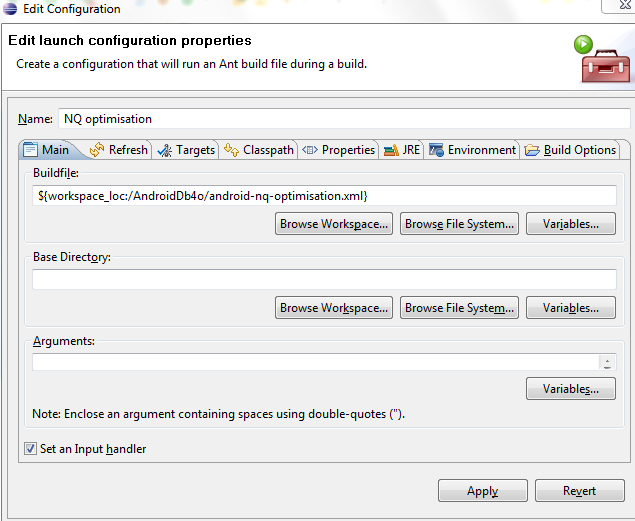
\includegraphics[width=\maxwidth]{images/ref-platform-specific-issues-android-ant-main.png}
\end{center}
Then go to the 'Properties'-tab. There add a new property 'android.platform' which points to the right Android-platform and version-path. You can find the platforms in you Android-SDK. The platforms are in the folder 'platforms' in the Android SDK. For example when your using the API-level 7 the platform is in the folder 'AndroidSDK/platforms/android-7'

\begin{center}
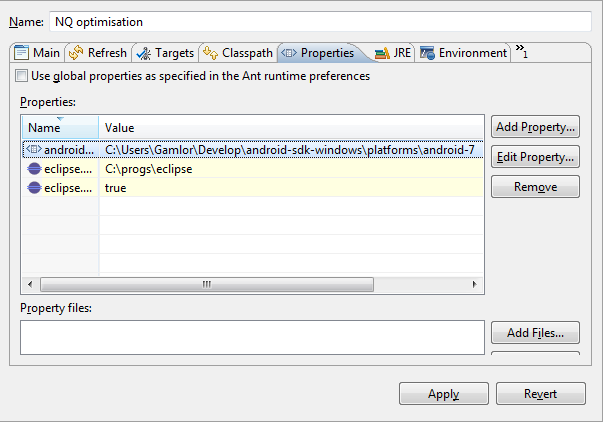
\includegraphics[width=\maxwidth]{images/ref-platform-specific-issues-android-ant-propeties.png}
\end{center}
Apply all settings. The last step is to place the new created builder between the 'Java Builder' and the 'Android Package Builder':

\begin{center}
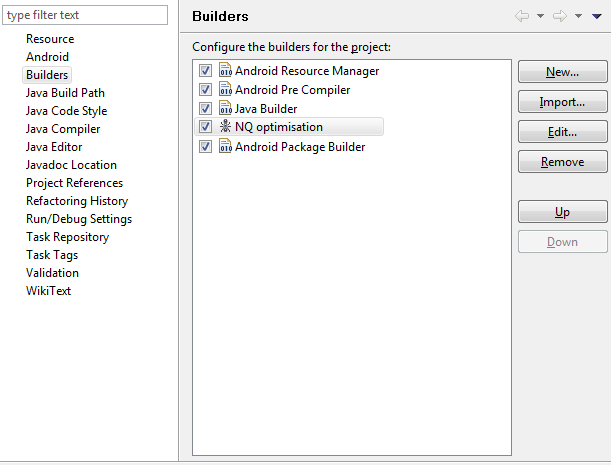
\includegraphics[width=\maxwidth]{images/ref-platform-specific-issues-android-builders.png}
\end{center}
\subsubsection*{Integrating in the Regular Build}

You simply can include the enhancer step into the regular Android build. For that include the enhancer Ant script in the build.xml and let it run during the compilation phase:

\begin{lstlisting}
<import file="${sdk.dir}/tools/ant/build.xml" />

<!-- Add the db4o step below the predefined android targets -->
<import file="android-db4o-optimisation.xml" />

<target name="-post-compile" depends="enhance">
</target>
\end{lstlisting}

{\small\itshape build.xml: Run the enhancer step during the build\par}
\medskip

\subsection{Comparison With SQLite}
\label{ref:platform-specific-issues-android-comparison-with-sqlite}

\href{http://code.google.com/android/}{Android} is a new complete, open and free mobile platform. Android offers developers a Java based software developer kit with lots of helpful APIs, including geolocational services. Of course, there is a database support as well: Android has a built-in support for SQLite database. The basic API is similar to standard JDBC API, with some additional helpful methods\newline{}

It may look better than SQL, but if you look closer it still has the same issues. Queries are specified as strings, so we still stay with a problem of run-time checking instead of compile-time. Furthermore you still need to map between your object-model and the relational SQLite database.

Luckily even for this very early Android release we already have an alternative - db4o. db4o runs on Android out of the box and produces very competitive results as well. The following examples compare db4o and SQLite usage for basic operations.

\begin{itemize}
\item \hyperref[ref:platform-specific-issues-android-general-info]{General Info} (p.~\pageref{ref:platform-specific-issues-android-general-info})
\item \hyperref[ref:platform-specific-issues-android-opening-a-database]{Opening A Database} (p.~\pageref{ref:platform-specific-issues-android-opening-a-database})
\item \hyperref[ref:platform-specific-issues-android-storing-data]{Storing Data} (p.~\pageref{ref:platform-specific-issues-android-storing-data})
\item \hyperref[ref:platform-specific-issues-android-retrieving-data]{Retrieving Data} (p.~\pageref{ref:platform-specific-issues-android-retrieving-data})
\item \hyperref[ref:platform-specific-issues-android-changing-data]{Changing Data} (p.~\pageref{ref:platform-specific-issues-android-changing-data})
\item \hyperref[ref:platform-specific-issues-android-deleting-data]{Deleting Data} (p.~\pageref{ref:platform-specific-issues-android-deleting-data})
\item \hyperref[ref:platform-specific-issues-android-backup]{Backup} (p.~\pageref{ref:platform-specific-issues-android-backup})
\item \hyperref[ref:platform-specific-issues-android-closing-a-database]{Closing A Database} (p.~\pageref{ref:platform-specific-issues-android-closing-a-database})
\item \hyperref[ref:platform-specific-issues-android-schema-evolution]{Schema Evolution} (p.~\pageref{ref:platform-specific-issues-android-schema-evolution})
\end{itemize}

\subsubsection{General Info}
\label{ref:platform-specific-issues-android-general-info}

Both db4o and SQLite are embedded databases, i.e. they run within an application process, removing the overhead associated with a client-server configuration, although db4o can also be used in client-server mode. Both db4o and SQLite offer zero-configuration run modes, which allows to get the database up and running immediately.

\paragraph*{Access Control}

SQLite relies solely on the file system for its database permissions and has no concept of user accounts. SQLite has database-level locks and does not support client/server mode.

db4o can use encryption or client/server mode for user access control. Client/server can also be used in embedded mode, i.e on the same device.

\paragraph*{Referential Integrity}

Traditionally referential integrity in relational databases is implemented with the help of foreign keys. However SQLite \href{http://www.sqlite.org/omitted.htm}{does not support} this feature. In db4o referential integrity is imposed by the object model, i.e. you can't reference an object that does not exist.

\paragraph*{Transactions}

Both db4o and SQLite support ACID transactions.

In db4o all the work is transactional: transaction is implicitly started when the database is open and closed either by explicit commit() call or by close() call through implicit commit. Data is protected from system crash during all application lifecycle. If a crash occurs during commit itself, the commit will be restarted when the system is up again if the system had enough time to write the list of changes, otherwise the transaction will be rolled back to the last safe state.

In SQLite autocommit feature is used by default: transaction is started when a SQL command other than SELECT is executed and commit is executed as soon as pending operation is finished. Explicit BEGIN and END TRANSACTION(COMMIT) or ROLLBACK can be used alternatively to specify user-defined transaction limits. Database crash always results in pending transaction rollback. Nested transactions are not supported.

\paragraph*{Database Size}

Though embeddable db4o and SQLite support big database files:

\begin{itemize}
\item db4o up to 256 GB
\item SQLite up to 2TB
\end{itemize}

all the data is stored in a single database file. db4o also supports clustered databases.

\subsubsection{Opening a Database}
\label{ref:platform-specific-issues-android-opening-a-database}

Opening the database is very similar.

\paragraph*{SQLite}

Opening a SQLite database is very easy. However is necessary to generate the schema for the database.

\begin{lstlisting}
SQLiteDatabase db = _context.openOrCreateDatabase(DATABASE_NAME,
        Context.MODE_PRIVATE, null);
\end{lstlisting}

{\small\itshape SqlExample.java: opening SQLite database\par}
\medskip

\begin{lstlisting}
db.execSQL("CREATE TABLE IF NOT EXISTS " + DB_TABLE_PILOT + " ("
        + "id INTEGER PRIMARY KEY AUTOINCREMENT, "
        + "name TEXT NOT NULL, points INTEGER NOT NULL);");
// Foreign key constraint is parsed but not enforced
// Here it is used for documentation purposes
db.execSQL("CREATE TABLE IF NOT EXISTS " + DB_TABLE_CAR + " ("
        + "id INTEGER PRIMARY KEY AUTOINCREMENT, "
        + "model TEXT NOT NULL, pilot INTEGER NOT NULL,"
        + "FOREIGN KEY (pilot)"
        + "REFERENCES pilot(id) ON DELETE CASCADE);");
db.execSQL("CREATE INDEX IF NOT EXISTS CAR_PILOT ON " + DB_TABLE_CAR
        + " (pilot);");
\end{lstlisting}

{\small\itshape SqlExample.java: SQLite create the schema\par}
\medskip

\paragraph*{db4o}

Opening a db4o database is easy. First you need to create a file which is in the context of the application. Then you can open the database. To be faster, we configure additional indexes.

\begin{lstlisting}
String filePath = context.getFilesDir() + "/android.db4o";
ObjectContainer db = Db4oEmbedded.openFile(configure(), filePath);
\end{lstlisting}

{\small\itshape Db4oExample.java: open a db4o database\par}
\medskip

\begin{lstlisting}
EmbeddedConfiguration configuration = Db4oEmbedded.newConfiguration();
      configuration.common().add(new AndroidSupport());
configuration.common().objectClass(Car.class).objectField("pilot").indexed(true);
configuration.common().objectClass(Pilot.class).objectField("points").indexed(true);
\end{lstlisting}

{\small\itshape Db4oExample.java: configure db4o\par}
\medskip

\paragraph*{Conclusion}

db4o code is a bit more compact, but the main advantage of db4o is in the fact that all APIs are pure java, they are compile-time checked and can be transferred into IDE templates (database opening should be a template as it most probably be the same for all your db4o applications including tests).

\subsubsection{Storing Data}
\label{ref:platform-specific-issues-android-storing-data}

Storing a car-object in is very-different in SQLite and db4o.

\paragraph*{SQLite}

\begin{lstlisting}
ContentValues initialValues = new ContentValues();

initialValues.put("id", number);
initialValues.put("name", "Tester");
initialValues.put("points", number);
db.insert(DB_TABLE_PILOT, null, initialValues);

initialValues = new ContentValues();

initialValues.put("model", "BMW");
initialValues.put("pilot", number);
db.insert(DB_TABLE_CAR, null, initialValues);
\end{lstlisting}

{\small\itshape SqlExample.java: store a car in SQLite\par}
\medskip

\paragraph*{db4o}

\begin{lstlisting}
Car car = new Car("BMW");
car.setPilot(new Pilot("Tester", points));
container.store(car);
\end{lstlisting}

{\small\itshape Db4oExample.java: store a car in db4o\par}
\medskip

\paragraph*{Conclusion}

You can see that db4o handles adding objects to the database in a much more elegant way - \#store(object) method is enough. In SQLite case it is much more difficult as you mush store different objects into different tables. Some of the additional work that SQLite developer will have to do is not visible in this example, i.e:

\begin{itemize}
\item the developer will have to ensure that the sequence of insert commands starts from children objects and goes up to the parent (this can be a really difficult task for relational models including lots of foreign key dependencies);
\item in most cases the data for insertion will come from business objects, which will mean that the object model will have to be transferred to relational model.
\end{itemize}

\subsubsection{Retrieving Data}
\label{ref:platform-specific-issues-android-retrieving-data}

In order to test the retrieval abilities of both databases we will try to select a car with a pilot having15 points:

\paragraph*{SQLite}

\begin{lstlisting}
SQLiteDatabase db = database();
Cursor cursor = db.rawQuery(
        "SELECT c.model, p.name, p.points, r.id, r.year" + " FROM "
                + DB_TABLE_CAR + " c, " + DB_TABLE_PILOT + " p "
                + "WHERE c.pilot = p.id AND p.points = ?;",
        new String[] { "15" });
cursor.moveToFirst();

Pilot pilot = new Pilot();
pilot.setName(cursor.getString(1));
pilot.setPoints(cursor.getInt(2));

Car car = new Car();
car.setModel(cursor.getString(0));
car.setPilot(pilot);
\end{lstlisting}

{\small\itshape SqlExample.java: select a car from SQLite\par}
\medskip

\paragraph*{db4o}

\begin{lstlisting}
ObjectContainer db = database();
ObjectSet<Car> cars = db.query(new Predicate<Car>() {
    @Override
    public boolean match(Car car) {
        return car.getPilot().getPoints() == 15;
    }
});

Car car = cars.get(0);
\end{lstlisting}

{\small\itshape Db4oExample.java: select a car from db4o\par}
\medskip

\paragraph*{Conclusion}

The db4o native queries are typesafe. This is a huge benefit, since the compiler can detect errors and the IDE help you with the refactoring. In the example above you can see that SQLite needs a lot of additional code to transfer the retrieved data into application's objects, whereas db4o does not need this code at all, as the result is already a collection of objects.

\subsubsection{Changing Data}
\label{ref:platform-specific-issues-android-changing-data}

For this test we will select and update a car with a new pilot, where existing pilot has 15 points:

\paragraph*{SQLite}

\begin{lstlisting}
SQLiteDatabase db = database();
db.execSQL("INSERT INTO REG_RECORDS (id,year) VALUES ('A1', DATETIME('NOW'))");

ContentValues updateValues = new ContentValues();
updateValues.put("reg_record", "A1");
int count = db.update(DB_TABLE_CAR, updateValues,
        "pilot IN (SELECT id FROM " + DB_TABLE_PILOT
                + " WHERE points = 15)", null);
if (count == 0) {
    logToConsole(0, "Car not found, refill the database to continue.",
            false);
} else {
    Cursor c = db.rawQuery("SELECT c.model, r.id, r.year from car c, "
            + "REG_RECORDS r, pilot p where c.reg_record = r.id "
            + "AND c.pilot = p.id AND p.points = 15;", null);
    if (c.getCount() == 0) {
        logToConsole(0,
                "Car not found, refill the database to continue.",
                false);
        return;
    }
    c.moveToFirst();
    String date = c.getString(2);
    
    Date dt = parseDate(date);
    RegistrationRecord record = new RegistrationRecord(c.getString(1),dt);
    
    Car car = new Car();
    car.setModel(c.getString(0));
    car.setRegistration(record);
    logToConsole(startTime, "Updated Car (" + car + "): ", true);
}
\end{lstlisting}

{\small\itshape SqlExample.java: update a car with SQLite\par}
\medskip

\paragraph*{db4o}

\begin{lstlisting}
ObjectContainer container = database();
if (container != null){
    ObjectSet<Car>  result = container.query(new Predicate<Car>(){
        @Override
        public boolean match(Car car) {
            return car.getPilot().getPoints()==15;
        }
        
    });
    if (!result.hasNext()){
        logToConsole(0, "Car not found, refill the database to continue.", false);
    } else {
        Car car = result.next();
        logToConsole(startTime, "Selected Car (" + car + "): ", false);
        startTime = System.currentTimeMillis();
        car.setRegistration(new RegistrationRecord("A1", new Date()));
        logToConsole(startTime, "Updated Car (" + car + "): ", true);
    }            
}
\end{lstlisting}

{\small\itshape Db4oExample.java: update a car with db4o\par}
\medskip

\paragraph*{Conclusion}

In this example db4o and SQLite actually behave quite differently. For SQLite in order to update a pilot in an existing car in the database the following actions are needed:

\begin{enumerate}
\item A new pilot should be created and saved to the database.
\item New pilot's primary key (101) should be retrieved (not shown in this example, but is necessary for a real database application).
\item An update statement should be issued to replace pilot field in the car table.
\end{enumerate}

For db4o database the sequence will be the following:

\begin{enumerate}
\item Retrieve the car from the database
\item Update the car with a new pilot object
\end{enumerate}

As you can see the only benefit of SQLite API is that the car can be selected and updated in one statement. But in the same time there are serious disadvantages:

\begin{itemize}
\item A new pilot record should be created absolutely separately (in a real database will also include ORM)
\item The pilot's ID needs to be retrieved separately (we must sure that it is a correct id)
\end{itemize}

In db4o we avoid these disadvantages as creating new pilot and updating the car value are actually combined in one atomic operation.

\subsubsection{Deleting Data}
\label{ref:platform-specific-issues-android-deleting-data}

The following methods will delete a car with a pilot having 5 points from each database:

\paragraph*{SQLite}

\begin{lstlisting}
SQLiteDatabase db = database();
db.delete(DB_TABLE_CAR,
        "pilot in (select id from pilot where points = ?)",
        new String[]{"5"});
\end{lstlisting}

{\small\itshape SqlExample.java: delete a car with SQLite\par}
\medskip

\paragraph*{db4o}

\begin{lstlisting}
ObjectContainer db = database();
ObjectSet<Car> cars = db.query(new Predicate<Car>() {
    public boolean match(Car car) {
        return car.getPilot().getPoints()==5;
    }            
});
for(Car car : cars){
    db.delete(car);
}
\end{lstlisting}

{\small\itshape Db4oExample.java: delete a car with db4o\par}
\medskip

\paragraph*{Conclusion}

In this example db4o code looks much longer. But should we consider it a disadvantage? My opinion is - No. Of course, SQLite seems to handle the whole operation in just one statement: db.delete(). But if you look attentively you will see that basically this statement just transfers all the difficult job to SQL: SQL statement should select a pilot with a given condition, then find a car. Using SQL can look shorter but it has a great disadvantage - it uses strings. So what will happen if the statement is wrong? You will never notice it till somebody in the running application will cause this statement to execute. Even then you might not see the reason immediately. The same applies to the schema changes - you may not even notice that you are using wrong tables and fields.

db4o helps to avoid all the above mentioned problems: query syntax is completely compile-checked and schema evolution will be spotted immediately by the compiler, so that you would not need to rely on code search and replace tools.

\subsubsection{Backup}
\label{ref:platform-specific-issues-android-backup}

\paragraph*{SQLite}

SQLite does not support a special API to make a backup. However, as you remember SQLite database is stored in a single database file, so the backup can be simply a matter of copying the database file. Unfortunately, this can't be done if the database is in use. In this case you can use \href{http://code.google.com/android/reference/adb.htm}{Android Debug Bridge} (adb) tool to access sqlite3 command-line application, which has .dump command for backing up database contents while the database is in use:

\begin{lstlisting}
E:\>adb shell
# sqlite3 /data/data/com.db4odoc.android.compare/databases/android.db
sqlite3 /data/data/com.db4odoc.android.compare/databases/android.db
SQLite version 3.5.0
Enter ".help" for instructions
sqlite> .dump > android200711.dmp
.dump > android200711.dmp
BEGIN TRANSACTION;
COMMIT;
sqlite>.exit
.exit
# ^D
\end{lstlisting}

Ctrl+D command is used to close adb session.

\paragraph*{db4o}

On db4o a ExtObjectContainer\#backup call is used to backup a database in use. \hyperref[ref:advanced-topics-backup]{See "Backup"} (p.~\pageref{ref:advanced-topics-backup})

\subsubsection{Closing a Database}
\label{ref:platform-specific-issues-android-closing-a-database}

The following methods will close SQLite and db4o database accordingly:

\paragraph*{SQLite}

\begin{lstlisting}
_db.close();
\end{lstlisting}

{\small\itshape SqlExample.java: close SQLite\par}
\medskip

\paragraph*{db4o}

\begin{lstlisting}
container.close();
\end{lstlisting}

{\small\itshape Db4oExample.java: close db4o\par}
\medskip

\subsubsection{Schema Evolution}
\label{ref:platform-specific-issues-android-schema-evolution}

When a new application development is considered it is important to think about its evolution. What happens if your initial model does not suffice and you need changes or additions? Let's look how db4o and SQLite applications can handle it.

To keep the example simple, let's add a registration record to our car:

\begin{lstlisting}
private RegistrationRecord registration;
   
public RegistrationRecord getRegistration() {
    return registration;
}

public void setRegistration(RegistrationRecord registration) {
    this.registration = registration;
}
\end{lstlisting}

{\small\itshape Car.java: Add a new field to the car\par}
\medskip

Ok, the application is changed to take care for the new class. What about our databases?

\subparagraph*{Schema Evolution in db4o}

db4o supports such schema change on the fly: we can select values and update the new field too:

\begin{lstlisting}
ObjectContainer container = database();
if (container != null){
    ObjectSet<Car>  result = container.query(new Predicate<Car>(){
        @Override
        public boolean match(Car car) {
            return car.getPilot().getPoints()==15;
        }
        
    });
    if (!result.hasNext()){
        logToConsole(0, "Car not found, refill the database to continue.", false);
    } else {
        Car car = result.next();
        logToConsole(startTime, "Selected Car (" + car + "): ", false);
        startTime = System.currentTimeMillis();
        car.setRegistration(new RegistrationRecord("A1", new Date()));
        logToConsole(startTime, "Updated Car (" + car + "): ", true);
    }            
}
\end{lstlisting}

{\small\itshape Db4oExample.java: update a car with db4o\par}
\medskip

\subparagraph*{Schema Evolution in SQLite}

For SQLite database model should be synchronized with the object model:

\begin{lstlisting}
db.execSQL("CREATE TABLE IF NOT EXISTS REG_RECORDS ("
        + "id TEXT PRIMARY KEY, year DATE);");
db.execSQL("CREATE INDEX  IF NOT EXISTS  IDX_REG_RECORDS ON REG_RECORDS (id);");
db.execSQL("ALTER TABLE " + DB_TABLE_CAR + " ADD reg_record TEXT;");
\end{lstlisting}

{\small\itshape SqlExample.java: upgrade schema in SQLite\par}
\medskip

Now we can try to retrieve and update records:

\begin{lstlisting}
SQLiteDatabase db = database();
db.execSQL("INSERT INTO REG_RECORDS (id,year) VALUES ('A1', DATETIME('NOW'))");

ContentValues updateValues = new ContentValues();
updateValues.put("reg_record", "A1");
int count = db.update(DB_TABLE_CAR, updateValues,
        "pilot IN (SELECT id FROM " + DB_TABLE_PILOT
                + " WHERE points = 15)", null);
if (count == 0) {
    logToConsole(0, "Car not found, refill the database to continue.",
            false);
} else {
    Cursor c = db.rawQuery("SELECT c.model, r.id, r.year from car c, "
            + "REG_RECORDS r, pilot p where c.reg_record = r.id "
            + "AND c.pilot = p.id AND p.points = 15;", null);
    if (c.getCount() == 0) {
        logToConsole(0,
                "Car not found, refill the database to continue.",
                false);
        return;
    }
    c.moveToFirst();
    String date = c.getString(2);
    
    Date dt = parseDate(date);
    RegistrationRecord record = new RegistrationRecord(c.getString(1),dt);
    
    Car car = new Car();
    car.setModel(c.getString(0));
    car.setRegistration(record);
    logToConsole(startTime, "Updated Car (" + car + "): ", true);
}
\end{lstlisting}

{\small\itshape SqlExample.java: update a car with SQLite\par}
\medskip

\subparagraph*{Conclusion}

You can see that schema evolution is much easier with db4o. But the main difficulty that is not visible from the example is that schema evolution with SQLite database can potentially introduce a lot of bugs that will be difficult to spot. For more information see \hyperref[ref:advanced-topics-refactoring-and-schema-evolution]{Refactoring and Schema Evolution} (p.~\pageref{ref:advanced-topics-refactoring-and-schema-evolution}).

\subsection{Proguard}
\label{ref:platform-specific-issues-android-proguard}

The Android SDK includes Proguard to shrink the size of the application by removing unused stuff, shorting names and other optimisations.

db4o relies heavily on reflection, which can lead to major issues when code is processed with Proguard. db4o has not been tested under such a environment. When you're using Proguard you need to test yourself if your application is still working.

You should to exclude all persisted classes from the shrinking process, because db4o manages objects by their name. Therefore db4o will have issue when those name changes by the shrinking process. Read the \href{http://proguard.sourceforge.net/index.html\#/manual/usage.html}{Proguard documentation} for the right configuration. For example when your persisted classes in a certain package you can exclude them like this:

\begin{lstlisting}
########################
-keep class com.db4odoc.android.**
-keepnames class com.db4odoc.android.**
-keepclassmembers class com.db4odoc.android.** {
    !static !transient <fields>;
    !private <fields>;
    !private <methods>;
}
\end{lstlisting}

{\small\itshape proguard.cfg: Keep persisted classes intact\par}
\medskip

To be on the save side you should keep all db4o classes in the original state. Especially since db4o stores some internal data structures which shouldn't be renamed.

\begin{lstlisting}
########################
## Monitoring requires JMX, which is not available on Android
-dontwarn com.db4o.monitoring.*
-dontwarn com.db4o.cs.monitoring.*
-dontwarn com.db4o.internal.monitoring.*

## Ant is usually not used in a running app
-dontwarn com.db4o.instrumentation.ant.*
-dontwarn com.db4o.ta.instrumentation.ant.*

## Keep internal classes.
-keep class com.db4o.** { *; }
\end{lstlisting}

{\small\itshape proguard.cfg: keep db4o intact\par}
\medskip

\section{db4o On Java Platforms}
\label{ref:platform-specific-issues-db4o-on-java-platforms}

\subsection*{All Java}

\begin{itemize}
\item root package is com.db4o
\end{itemize}

\subsection*{JDK 1.5 or newer}

\begin{itemize}
\item Generics support introduced in JDK1.5 makes db4o Native Query syntax much simpler: \texttt{List \textless{}Pilot\textgreater{} pilots = db.query(new Predicate \textless{}Pilot\textgreater{} () \{ public boolean match(Pilot pilot) \{ return pilot.getPoints() == 100;\}\});}
\item following JDK5 annotations db4o introduces its own annotations.
\item you can use built-in enums
\item db4o for JDK5 also has replication support.
\end{itemize}

\subsection*{Android}

Read about how to use \hyperref[ref:platform-specific-issues-android]{db4o on Android here} (p.~\pageref{ref:platform-specific-issues-android}).

\section{Security Requirements On Java Platform}
\label{ref:platform-specific-issues-security-requirements-on-java-platform}

Java Security Manager can be used to specify Java application security permissions. It is usually provided by web-browsers and web-servers for applet and servlet execution, however any Java application can make use of a security manager. For example, to use the default security manager you will only need to pass \texttt{-Djava.security.manager} option to JVM command line. Custom security managers can be created and utilized as well (please refer to Java documentation for more information).

If you are going to use db4o in a Tomcat servlet container you will need to grant some additional permissions in \{CATALINA\_HOME\}/conf/catalina.policy file:

\begin{lstlisting}
// The permissions granted to the context 
WEB-INF/classes directory 
grant codeBase "file:${catalina.home}/webapps/{your_db4o_application}/WEB-INF/classes/-" 
{ 
    permission java.util.PropertyPermission "user.home", "read"; 
    permission java.util.PropertyPermission "java.fullversion", "read";    
    permission java.io.FilePermission "path_to_db4o_database_folder", "read";    
    permission java.io.FilePermission "path_to_db4o_database_file", "read, write"; 
}; 
// The permissions granted to the context WEB-INF/lib directory, containing db4o jar 
grant codeBase "file:${catalina.home}/webapps/{your_db4o_application}/WEB-INF/lib/-" 
{    
    permission java.io.FilePermission "path_to_db4o_database_file", "read, write"; 
};
            
\end{lstlisting}

An example catalina.policy file:

\begin{lstlisting}
// Licensed to the Apache Software Foundation (ASF) under one or more
// contributor license agreements.  See the NOTICE file distributed with
// this work for additional information regarding copyright ownership.
// The ASF licenses this file to You under the Apache License, Version 2.0
// (the "License"); you may not use this file except in compliance with
// the License.  You may obtain a copy of the License at
//
//     http://www.apache.org/licenses/LICENSE-2.0
//
// Unless required by applicable law or agreed to in writing, software
// distributed under the License is distributed on an "AS IS" BASIS,
// WITHOUT WARRANTIES OR CONDITIONS OF ANY KIND, either express or implied.
// See the License for the specific language governing permissions and
// limitations under the License.

// ============================================================================
// catalina.corepolicy - Security Policy Permissions for Tomcat 6
//
// This file contains a default set of security policies to be enforced (by the
// JVM) when Catalina is executed with the "-security" option.  In addition
// to the permissions granted here, the following additional permissions are
// granted to the codebase specific to each web application:
//
// * Read access to the document root directory
//
// $Id: catalina.policy 609294 2008-01-06 11:43:46Z markt $
// ============================================================================

// ========== SYSTEM CODE PERMISSIONS =========================================

// These permissions apply to javac
grant codeBase "file:${java.home}/lib/-" {
        permission java.security.AllPermission;
};

// These permissions apply to all shared system extensions
grant codeBase "file:${java.home}/jre/lib/ext/-" {
        permission java.security.AllPermission;
};

// These permissions apply to javac when ${java.home] points at $JAVA_HOME/jre
grant codeBase "file:${java.home}/../lib/-" {
        permission java.security.AllPermission;
};

// These permissions apply to all shared system extensions when
// ${java.home} points at $JAVA_HOME/jre
grant codeBase "file:${java.home}/lib/ext/-" {
        permission java.security.AllPermission;
};

// ========== CATALINA CODE PERMISSIONS =======================================

// These permissions apply to the daemon code
grant codeBase "file:${catalina.home}/bin/commons-daemon.jar" {
        permission java.security.AllPermission;
};

// These permissions apply to the logging API
grant codeBase "file:${catalina.home}/bin/tomcat-juli.jar" {
        permission java.security.AllPermission;

        permission java.util.PropertyPermission "java.util.logging.config.class", "read";
        permission java.util.PropertyPermission "java.util.logging.config.file", "read";
        permission java.lang.RuntimePermission "shutdownHooks";
        permission java.io.FilePermission "${catalina.base}${file.separator}conf${file.separator}logging.properties", "read";
        permission java.util.PropertyPermission "catalina.base", "read";
        permission java.util.logging.LoggingPermission "control";
        permission java.io.FilePermission "${catalina.base}${file.separator}logs", "read, write";
        permission java.io.FilePermission "${catalina.base}${file.separator}logs${file.separator}*", "read, write";
        permission java.lang.RuntimePermission "getClassLoader";
        // To enable per context logging configuration, permit read access to the appropriate file.
        // Be sure that the logging configuration is secure before enabling such access
        // eg for the examples web application:
        // permission java.io.FilePermission "${catalina.base}${file.separator}webapps${file.separator}examples${file.separator}WEB-INF${file.separator}classes${file.separator}logging.properties", "read";
};

// These permissions apply to the server startup code
grant codeBase "file:${catalina.home}/bin/bootstrap.jar" {
        permission java.security.AllPermission;
};

// These permissions apply to the servlet API classes
// and those that are shared across all class loaders
// located in the "lib" directory
grant codeBase "file:${catalina.home}/lib/-" {
        permission java.security.AllPermission;
};

// ========== WEB APPLICATION PERMISSIONS =====================================

// These permissions are granted by default to all web applications
// In addition, a web application will be given a read FilePermission
// and JndiPermission for all files and directories in its document root.
grant { 
    // Required for JNDI lookup of named JDBC DataSource's and
    // javamail named MimePart DataSource used to send mail
    permission java.util.PropertyPermission "java.home", "read";
    permission java.util.PropertyPermission "java.naming.*", "read";
    permission java.util.PropertyPermission "javax.sql.*", "read";

    // OS Specific properties to allow read access
    permission java.util.PropertyPermission "os.name", "read";
    permission java.util.PropertyPermission "os.version", "read";
    permission java.util.PropertyPermission "os.arch", "read";
    permission java.util.PropertyPermission "file.separator", "read";
    permission java.util.PropertyPermission "path.separator", "read";
    permission java.util.PropertyPermission "line.separator", "read";

    // JVM properties to allow read access
    permission java.util.PropertyPermission "java.version", "read";
    permission java.util.PropertyPermission "java.vendor", "read";
    permission java.util.PropertyPermission "java.vendor.url", "read";
    permission java.util.PropertyPermission "java.class.version", "read";
    permission java.util.PropertyPermission "java.specification.version", "read";
    permission java.util.PropertyPermission "java.specification.vendor", "read";
    permission java.util.PropertyPermission "java.specification.name", "read";

    permission java.util.PropertyPermission "java.vm.specification.version", "read";
    permission java.util.PropertyPermission "java.vm.specification.vendor", "read";
    permission java.util.PropertyPermission "java.vm.specification.name", "read";
    permission java.util.PropertyPermission "java.vm.version", "read";
    permission java.util.PropertyPermission "java.vm.vendor", "read";
    permission java.util.PropertyPermission "java.vm.name", "read";

    // Required for OpenJMX
    permission java.lang.RuntimePermission "getAttribute";

    // Allow read of JAXP compliant XML parser debug
    permission java.util.PropertyPermission "jaxp.debug", "read";

    // Precompiled JSPs need access to this package.
    permission java.lang.RuntimePermission "accessClassInPackage.org.apache.jasper.runtime";
    permission java.lang.RuntimePermission "accessClassInPackage.org.apache.jasper.runtime.*";
    
    // Precompiled JSPs need access to this system property.
    permission java.util.PropertyPermission "org.apache.jasper.runtime.BodyContentImpl.LIMIT_BUFFER", "read";

};

// The permissions granted to the context WEB-INF/classes directory
grant codeBase "file:${catalina.home}/webapps/Db4oSite/WEB-INF/classes/-" {
   permission java.util.PropertyPermission "user.home", "read";  
   permission java.util.PropertyPermission "java.fullversion", "read";
   permission java.io.FilePermission "${user.home}${file.separator}db4o${file.separator}data", "read";
   permission java.io.FilePermission "${user.home}${file.separator}db4o${file.separator}data${file.separator}test.db4o.yap", "read, write";
};

grant codeBase "file:${catalina.home}/webapps/Db4oSite/WEB-INF/lib/-" {
   permission java.io.FilePermission "${user.home}${file.separator}db4o${file.separator}data${file.separator}test.db4o.yap", "read, write";
};

// You can assign additional permissions to particular web applications by
// adding additional "grant" entries here, based on the code base for that
// application, /WEB-INF/classes/, or /WEB-INF/lib/ jar files.
//
// Different permissions can be granted to JSP pages, classes loaded from
// the /WEB-INF/classes/ directory, all jar files in the /WEB-INF/lib/
// directory, or even to individual jar files in the /WEB-INF/lib/ directory.
//
// For instance, assume that the standard "examples" application
// included a JDBC driver that needed to establish a network connection to the
// corresponding database and used the scrape taglib to get the weather from
// the NOAA web server.  You might create a "grant" entries like this:
//
// The permissions granted to the context root directory apply to JSP pages.
// grant codeBase "file:${catalina.home}/webapps/examples/-" {
//      permission java.net.SocketPermission "dbhost.mycompany.com:5432", "connect";
//      permission java.net.SocketPermission "*.noaa.gov:80", "connect";
// };
//
// The permissions granted to the context WEB-INF/classes directory
// grant codeBase "file:${catalina.home}/webapps/examples/WEB-INF/classes/-" {
// };
//
// The permission granted to your JDBC driver
// grant codeBase "jar:file:${catalina.home}/webapps/examples/WEB-INF/lib/driver.jar!/-" {
//      permission java.net.SocketPermission "dbhost.mycompany.com:5432", "connect";
// };
// The permission granted to the scrape taglib
// grant codeBase "jar:file:${catalina.home}/webapps/examples/WEB-INF/lib/scrape.jar!/-" {
//      permission java.net.SocketPermission "*.noaa.gov:80", "connect";
// };
\end{lstlisting}

In order to avoid db4o DatabaseFileLocked exception you will also need to add some configuration before opening the object container:\newline{}

\texttt{Configuration config = Db4o.newConfiguration();\newline{}}

\texttt{config.lockDatabaseFile(false);\newline{}}

\texttt{ObjectContainer container = Db4o.openFile(config, dbfile.getPath());\newline{}}

Having done that, you can package and deploy your application. To enable the security configuration start Tomcat with the following command:\newline{}

\{CATALINA\_HOME\}/bin/catalina start -security \newline{}

\section{XML Import-Export}
\label{ref:platform-specific-issues-xml-import-export}

One of the most widely used platform independent formats of data exchange today is xml.

db4o does not provide any specific API to be used for XML import/export, but with the variety of XML serialization libraries available.

All that you need to export your database/query results is:

\begin{enumerate}
\item Retrieve objects from the database.
\item Serialize them in XML format using your favorite serialization API/library
\item Save XML stream (to a disc location, into memory, into another database).
\end{enumerate}

Import process is just the reverse:

\begin{enumerate}
\item Read the XML stream.
\item Create an objects from XML.
\item Save objects to db4o.
\end{enumerate}

Let's go through a simple example. We will use XStream library (\href{http://xstream.codehaus.org/}{http://xstream.codehaus.org/}) for object serialization, but any other tool capable of serializing objects into XML will do as well.

\begin{lstlisting}
ObjectContainer container = Db4oEmbedded.openFile("database.db4o");
try {
    Pilot[] pilots = container.query(Pilot.class).toArray(new Pilot[0]);
    XStream xstream = new XStream();
    OutputStream stream = new FileOutputStream("pilots.xml");
    try {
        xstream.toXML(pilots, stream);
    } finally {
        stream.close();
    }
} finally {
    container.close();
}
\end{lstlisting}

{\small\itshape XMLSerialisationExamples.java: Serialize to XML\par}
\medskip

After the method executes all car objects from the database will be stored in the export file as an array. Note that child objects (Pilot) are stored as well without any additional settings. You can check the created XML file to see how it looks like.

Now we can clean the database and try to recreate it from the XML file:

\begin{lstlisting}
ObjectContainer container = Db4oEmbedded.openFile("database.db4o");
try {
    XStream xstream = new XStream();
    InputStream stream = new FileInputStream("pilots.xml");
    try {
        Pilot[] pilots = (Pilot[]) xstream.fromXML(stream);
        for (Pilot pilot : pilots) {
            container.store(pilot);
        }
    } finally {
        stream.close();
    }
} finally {
    container.close();
}
\end{lstlisting}

{\small\itshape XMLSerialisationExamples.java: Read objects from XML\par}
\medskip

Obviously there is much more to XML serialization: renaming fields, storing collections, selective persistence etc. You should be able to find detailed description together with the serialization library, which you will use.

\section{OSGi}
\label{ref:platform-specific-issues-database-for-osgi}

db4o can run in an OSGi environment. db4o jars have a OSGi manifest so that you can use them in your project.

\subsection*{Using db4o with OSGi}

In principal you can use db4o in OSGi without any special configuration, as long as the stored objects and db4o are loaded with the same OSGi classloader.

However as soon as you're using multiple bundles, and therefore multiple classloaders, you need to configure db4o. You can \hyperref[ref:configuration-common-reflector]{specify the class-loader explicitly} (p.~\pageref{ref:configuration-common-reflector}) for db4o, or even use multiple class-loaders. This way you can lookup in multiple class-loaders for your class. First write an implementation of the JdkLoader interface:

\begin{lstlisting}
class OSGiLoader implements JdkLoader{
    private final Bundle[] bundlesToLookIn;

    OSGiLoader(Bundle... bundlesToLookIn) {
        this.bundlesToLookIn = bundlesToLookIn;
    }

    public Class loadClass(String s) {
        for (Bundle bundle : bundlesToLookIn) {
            try {
                return bundle.loadClass(s);
            } catch (ClassNotFoundException e) {
                // just retry on other bundles
            }
        }
        try {
            return getClass().getClassLoader().loadClass(s);
        } catch (ClassNotFoundException e) {
            return null;
        }
    }

    public Object deepClone(Object o) {
        return new OSGiLoader(bundlesToLookIn);
    }
}
\end{lstlisting}

{\small\itshape UsingDb4oDirectly.java: Load classes from multiple bundles\par}
\medskip

After that you can use your implementation to load classes for db4o:

\begin{lstlisting}
// Specify the bundles from which the classes are used to store objects
Bundle[] bundles = new Bundle[]{bundleContext.getBundle()};
EmbeddedConfiguration configuration = Db4oEmbedded.newConfiguration();
configuration.common()
        .reflectWith(new JdkReflector(new OSGiLoader(bundles)));
\end{lstlisting}

{\small\itshape UsingDb4oDirectly.java: Db4o with a special OSGi loader\par}
\medskip

Note also that some db4o jars have a dependency on Ant and need an Ant bundle in your OSGi application to use all features.

\subsection*{Using the db4o OSGi package}

An alternative is to use the db4o OSGi package, which is in the db4o--X.XX-osgi.jar and includes all dependencies. \hyperref[ref:dependency-overview]{See "Dependency Overview"} (p.~\pageref{ref:dependency-overview}). This provides a OSGi service which creates a db4o instance for you. It configures db4o in such a way that classes are loaded from the requesting OSGi service.

\begin{lstlisting}
ServiceReference reference = bundleContext.getServiceReference("com.db4o.osgi.Db4oService");
Db4oService db4oService = (Db4oService) bundleContext.getService(reference);
ObjectContainer container = db4oService.openFile("database.db4o");
\end{lstlisting}

{\small\itshape UsingDb4oViaService.java: Get db4o osgi service\par}
\medskip


% Converted from reference/DB4OFlare (MadCap Flare, Java target)

\chapter{Usage Pitfalls}
\label{ref:usage-pitfalls}

The db4o team tries hard to make the db4o as easy to use as possible. However there are still some pitfalls.

When objects are only partially loaded and you run into null pointer exceptions, then you ran into not activated objects. This is a common issue. \hyperref[ref:usage-pitfalls-activation-depth]{See "The Activation Pitfall"} (p.~\pageref{ref:usage-pitfalls-activation-depth})

When updates are not stored then you have issues with the update-depth. \hyperref[ref:usage-pitfalls-update-depth]{See "Update Depth Pitfall"} (p.~\pageref{ref:usage-pitfalls-update-depth})

db4o tries hard to store every object without any mapping. However in practice the mapping is not perfect. For UUID you should add a configuration to support them propertly. \hyperref[ref:advanced-topics-type-handling-uuid-support]{See "UUID Support"} (p.~\pageref{ref:advanced-topics-type-handling-uuid-support}). For big math types you need some additional configuration \hyperref[ref:usage-pitfalls-storing-bigdecimal]{See "Storing BigDecimal And BigInteger"} (p.~\pageref{ref:usage-pitfalls-storing-bigdecimal}). Also be careful with collections and avoid SQL-Types. \hyperref[ref:usage-pitfalls-special-type-handling]{See "Special Type Handling"} (p.~\pageref{ref:usage-pitfalls-special-type-handling})

In more complex Java environments you may run into class loading issues. \hyperref[ref:usage-pitfalls-classloader-and-generic-classes]{See "Classloader And Generic Classes"} (p.~\pageref{ref:usage-pitfalls-classloader-and-generic-classes})

There are a few dangerous practices which you really should avoid. \hyperref[ref:usage-pitfalls-dangerous-practices]{See "Dangerous Practices"} (p.~\pageref{ref:usage-pitfalls-dangerous-practices})

db4o has database size limit, which is by default 2 GByte. See how you can increase it. \hyperref[ref:usage-pitfalls-working-with-large-amounts-of-data]{See "Working With Large Amounts Of Data"} (p.~\pageref{ref:usage-pitfalls-working-with-large-amounts-of-data})

\section{Activation Depth Pitfall}
\label{ref:usage-pitfalls-activation-depth}

In order to work effectively with db4o you should understand the concept of \hyperref[ref:basics-activation]{Activation} (p.~\pageref{ref:basics-activation}). Activation controls the amount of objects loaded into the memory. There are two main pitfalls that you should be aware about.

\subsection*{Accessing Not Activated Objects}

One common pitfall is to access unactivated objects. This usually results in null pointer exceptions or invalid values. This happens when you navigate beyond the activated object-graph area. For example, we have a complex relationships and follow them:

\begin{lstlisting}
final Person jodie = queryForJodie(container);
Person julia = jodie.mother().mother().mother().mother().mother();
// This will print null
// Because julia is not activated
// and therefore all fields are not set
System.out.println(julia.getName());
// This will throw a NullPointerException.
// Because julia is not activated
// and therefore all fields are not set
String joannaName = julia.mother().getName();
\end{lstlisting}

{\small\itshape ActivationDepthPitfall.java: Run into not activated objects\par}
\medskip

This will result in a exception. Because by default db4o only activates objects up the a depth of 5. This means that when you load an object, that object and all objects which are reachable via 4 references are activated.

There are multiple solutions to this issue.

\begin{itemize}
\item Activate the object explicitly as you dive deeper into the object graph.
\item Increase the \hyperref[ref:configuration-common-activation-depth]{global activation-depth} (p.~\pageref{ref:configuration-common-activation-depth}).
\item Increase the activation-depth \hyperref[ref:configuration-objectclass-minimum-activation-depth]{for certain types} (p.~\pageref{ref:configuration-objectclass-minimum-activation-depth}).
\item Use wisely the \hyperref[ref:configuration-objectclass-cascade-on-activate]{cascading activation} (p.~\pageref{ref:configuration-objectclass-cascade-on-activate}).
\item The most elegant solution is \hyperref[ref:basics-activation-concept-transparent-activation-framework]{transparent activation} (p.~\pageref{ref:basics-activation-concept-transparent-activation-framework}). With transparent activation db4o takes care of activating object as you access them.
\end{itemize}

\subsection*{To High Activation Depth Or Two Many Cascade Activation}

Having a high activation-depth makes working with db4o much easier. However activation can take a long time with deeper object graphs and become a serious performance bottleneck. The same applies when using cascade activation on almost all types. To reduce the time spend on activating objects, you need to be more selective about what to activate and what not.

\begin{itemize}
\item Activate the object explicitly as you dive deeper into the object graph.
\item The most elegant solution is \hyperref[ref:basics-activation-concept-transparent-activation-framework]{transparent activation} (p.~\pageref{ref:basics-activation-concept-transparent-activation-framework}). With transparent activation db4o takes care of activating object as you access them.
\end{itemize}

\section{Update Depth Pitfall}
\label{ref:usage-pitfalls-update-depth}

db4o update behavior is regulated by \hyperref[ref:basics-update-concept]{Update Depth} (p.~\pageref{ref:basics-update-concept}). Understanding update depth will help you to improve performance and avoid unnecessary memory usage. A common pitfall is that the update-depth is to small and that the objects are not updated. In such cases you either need to explicitly store the related objects individually or \hyperref[ref:configuration-common-update-depth]{increase the update-depth} (p.~\pageref{ref:configuration-common-update-depth}).

For example in this code we add a new friend and store the object. Since a collection is also handled like a regular object, it is affected by the update-depth. In this example we only store the person-object, but not the friend-collection-object. Therefore with the default-update depth of one the update isn't store. In order to update this properly, you either need to set the update depth to two or store the friend-list explicitly.

\begin{lstlisting}
ObjectContainer container = Db4oEmbedded.openFile(DATABASE_FILE);
try {
    Person jodie = queryForJodie(container);
    jodie.add(new Person("Jamie"));
    // Remember that a collection is also a regular object
    // so with the default-update depth of one, only the changes
    // on the person-object are stored, but not the changes on
    // the friend-list.
    container.store(jodie);
} finally {
    container.close();
}
container = Db4oEmbedded.openFile(DATABASE_FILE);
try {
    Person jodie = queryForJodie(container);
    for (Person person : jodie.getFriends()) {
        // the added friend is gone, because the update-depth is to low
        System.out.println("Friend="+person.getName());
    }
} finally {
    container.close();
}
\end{lstlisting}

{\small\itshape UpdateDepthPitfall.java: Update doesn't work on collection\par}
\medskip

So for this example setting the update-depth to two will fix the issue. For lots of operation a update-depth of two is pretty reasonable. This allows you to update collections without storing them explicitly.

\begin{lstlisting}
EmbeddedConfiguration config = Db4oEmbedded.newConfiguration();
config.common().updateDepth(2);
ObjectContainer container = Db4oEmbedded.openFile(config,DATABASE_FILE);
\end{lstlisting}

{\small\itshape UpdateDepthPitfall.java: A higher update depth fixes the issue\par}
\medskip

When the update depth is set to a big value on objects with a deep reference hierarchy it will cause each update on the top-level object to trigger updates on the lower-level objects, which can impose a huge performance penalty.

Try \hyperref[ref:basics-update-concept-transparent-persistence]{transparent persistence} (p.~\pageref{ref:basics-update-concept-transparent-persistence}), which removes the issue of the update-depth completly.

\section{Storing BigDecimal And BigInteger}
\label{ref:usage-pitfalls-storing-bigdecimal}

\subsection*{Problem}

BigDecimal or BigInteger objects can't be stored by db4o with the default configuration because those object contains some transient state. You need to add big decimal support to db4o to store a BigDecimal or a BigInteger. \hyperref[ref:advanced-topics-type-handling-bigmath]{See "BigMath"} (p.~\pageref{ref:advanced-topics-type-handling-bigmath})

\section{Special Type Handling}
\label{ref:usage-pitfalls-special-type-handling}

For some often used types db4o implements a special type-handling. This can inflict some issues.

\subsection*{SQL-Date cannot be stored properly}

The java.sql.Date extends the standard java.util.Date-type. The date-type is treated like other value-types such as strings, integers etc. Unfortunatly this isn't true for the java.sql.Date-type. This also means that the SQL-date type cannot be store correctly. When you retrieve a SQL-Date type it will contain the wrong date.

The solution is to use only the normal JDK-Date. Theirs no reason to use the java.sql.Date-type.

\subsection*{Be Careful with own Collection-Types}

db4o uses \hyperref[ref:advanced-topics-type-handling-typehandlers]{special type-handlers} (p.~\pageref{ref:advanced-topics-type-handling-typehandlers}) for collections to improve efficiency. This also means that db4o makes some assumptions about the collection. It assumes that all collection-methods are implemented and work properly. This isn't true for special collections like the JDK unemployable collections or maybe for you own special collection.

For example this simple collection which doesn't implement all methods:

\begin{lstlisting}
class MyFixedSizeCollection<E> extends AbstractCollection<E>{
    private E[] items;

    public MyFixedSizeCollection(E[] items) {
        this.items = items;
    }

    @Override
    public Iterator<E> iterator() {
        return Arrays.asList(items).iterator();
    }

    @Override
    public int size() {
        return items.length;
    }
}
\end{lstlisting}

{\small\itshape MyFixedSizeCollection.java: This collection doesn't implement all collection methods\par}
\medskip

This collection will create exceptions when you try to load it. Because db4o uses the clear and add-methods on the collection.

\begin{lstlisting}
try {
    ObjectSet<CollectionHolder> holders = container.query(CollectionHolder.class);
    MyFixedSizeCollection<String> collection = holders.get(0).getNames();
} catch (Exception e) {
    // this will fail! The db4o collection-storage
    // assumes that collections support all operations of the collection interface.
    // db4o uses the regular collection-methods to restore the instance.
    e.printStackTrace();
}
\end{lstlisting}

{\small\itshape TypeHandlingEdgeCases.java: db4o fails to load partially implemented collections\par}
\medskip

\section{Classloader And Generic Classes}
\label{ref:usage-pitfalls-classloader-and-generic-classes}

db4o uses class information available from the classloader to store and recreate class objects. When a class definition is not available from the classloader db4o resolves to \hyperref[ref:advanced-topics-db4o-reflection-api-genericreflector]{Generic Objects} (p.~\pageref{ref:advanced-topics-db4o-reflection-api-genericreflector}), which represent the class information stored in object arrays. With this approach db4o is ready to function both with and without \hyperref[ref:client-server-server-without-persistent-classes-deployed]{class definitions available} (p.~\pageref{ref:client-server-server-without-persistent-classes-deployed}). However, the problem can appear when your application and db4o use different classloaders, because in this case db4o won't match objects in the database to their definitions in the runtime. In order to avoid this:

\begin{enumerate}
\item Make sure that your db4o lib is not in JRE or JDK lib folder. Libraries in these folders get a special classloader, which is unaware of your application classes. Instead put db4o library into any other suitable for you location and make it available to your application through CLASSPATH or using IDE provided methods.
\item If your application design does not guarantee that application classes and db4o will be loaded by the same classloader, specify the right classloader with setting \hyperref[ref:configuration-common-reflector]{the reflector explicitly.} (p.~\pageref{ref:configuration-common-reflector})
\end{enumerate}

The above-mentioned cases should be distinguished from a case when Java application uses a db4o database created from a .NET application. In this particular case .NET class definitions should be replaced by Java class definitions with the help of \hyperref[ref:configuration-common-alias]{Aliases} (p.~\pageref{ref:configuration-common-alias}).

\section{Dangerous Practices}
\label{ref:usage-pitfalls-dangerous-practices}

Db4o databases are well protected against corruption. However some specific configurations can make your database file vulnerable.

\begin{itemize}
\item \hyperref[ref:configuration-file-lock-database]{Disabling the file-lock} (p.~\pageref{ref:configuration-file-lock-database}). When two db4o instance write to the same database file at the same time, the database will be corrupted. Therefore you should avoid disabling this setting. You can safely disable the file-lock, when you're using the database in a \hyperref[ref:configuration-file-read-only]{read-only} (p.~\pageref{ref:configuration-file-read-only}) mode.
\item Using the \hyperref[ref:configuration-file-storage-nonflushingstorage]{non-flushing storage} (p.~\pageref{ref:configuration-file-storage-nonflushingstorage}). This storage will disable the flush-operation to the disk. While this improves the performance, it endangers consistent commits in a crash.
\item db4o cannot deal with some class-hierarchy-changes. You cannot add a class between two existing classes in the class-hierarchy. Or remove a class from the top of the class-hierarchy. \hyperref[ref:advanced-topics-refactoring-and-schema-evolution-refactoring-class-hierarchy]{See "Refactoring Class Hierarchy"} (p.~\pageref{ref:advanced-topics-refactoring-and-schema-evolution-refactoring-class-hierarchy})
\item You cannot change a field from a array to a simple field of the same type and back.This only applies when you change it from a type to the same array-type. So for example from a string to an array of strings. A change from string to an array of integer is fine. \hyperref[ref:advanced-topics-refactoring-and-schema-evolution-field-refactoring-limitation]{See "Field Refactoring Limitation"} (p.~\pageref{ref:advanced-topics-refactoring-and-schema-evolution-field-refactoring-limitation})
\end{itemize}

\section{Working With Large Amounts Of Data}
\label{ref:usage-pitfalls-working-with-large-amounts-of-data}

The following paragraphs highlight some information important for using db4o with large data.

\subsection*{Size of Database Files}

In the default setting, the maximum database file size is 2GB. You can increase this value by \hyperref[ref:configuration-file-block-size]{configuring the internal db4o block size} (p.~\pageref{ref:configuration-file-block-size}). The maximum possible size is 254GB.

You cannot change this setting for an existing database. In order to change it for an existing database, you need to \hyperref[ref:troubleshoot-increasing-the-maximum-database-file-size]{defragment the database} (p.~\pageref{ref:troubleshoot-increasing-the-maximum-database-file-size}).


% Converted from reference/DB4OFlare (MadCap Flare, Java target)

\chapter{Troubleshooting}
\label{ref:trouble-shooting}

Here are a few tips on troubleshooting issues with db4o.

\section{General Diagnostics}
\label{ref:trouble-shooting:general}

To get more diagnostics information you can register diagnostics listeners.

\begin{itemize}
\item \hyperref[ref:advanced-topics-diagnostics]{See "Diagnostics"} (p.~\pageref{ref:advanced-topics-diagnostics})
\item \hyperref[ref:advanced-topics-runtime-statistics]{See "Runtime Monitoring"} (p.~\pageref{ref:advanced-topics-runtime-statistics})
\end{itemize}

\section*{Investigate a Corrupt Database}

Take a look at this small guide which gives tips on how to deal with a corrupt database. \hyperref[ref:troubleshoot-corrupt-db]{See "Deal With a Corrupt Database"} (p.~\pageref{ref:troubleshoot-corrupt-db})

\section*{Performance and Scalability Issues}

If you experience issues with the performance of db4o take a look at this topic: \hyperref[ref:troubleshoot-speed-issues-html]{See "Performance and Scalability Issues"} (p.~\pageref{ref:troubleshoot-speed-issues-html})

\section{Ask for Help and Advice}
\label{ref:trouble-shooting:ask}

The original db4o forums no longer exist. If you hit a problem, see the db4o repository at \href{https://github.com/blakemcbride/db4o}{\nolinkurl{github.com/blakemcbride/db4o}}.

\section{Investigate a Corrupt Database}
\label{ref:troubleshoot-corrupt-db}

In general you should do regular \hyperref[ref:advanced-topics-backup]{backups} (p.~\pageref{ref:advanced-topics-backup}) of your database. db4o tries to do its best to never corrupt the database. However due to bugs or external reasons corruption can occur. Check also your configuration to not use \hyperref[ref:basics-acid-and-transactions-dangerous-practises]{any risky settings} (p.~\pageref{ref:basics-acid-and-transactions-dangerous-practises}).

If you have a corrupted database you may think about reporting it: \hyperref[ref:community-report-bugs]{See "Report Bugs"} (p.~\pageref{ref:community-report-bugs})

The fist step is to run the consistency check on your database. If the database is really corrupt you can try to restore at least some your data.

\subsection*{Consistency Check}

To run consistency checks use the com.db4o.consistency.ConsistencyChecker class, like this:

\begin{lstlisting}
java -cp db4o-8.1-all.jar com.db4o.consistency.ConsistencyChecker databaseFile.db4o
\end{lstlisting}

This consistency check doesn't check the content of objects. It only checks if the overall structure of the database file is still intact. Also it doesn't offer any repair functionality. It only tells you if the file is corrupted or not.

When the tool reports inconsistencies you've defiantly have a corrupted database. Then you should fall back to the latest backup or try to recover parts of the database.

In case the tool doesn't report any issues you maybe still have a corrupted object in your database. In that case you usually can read all intact objects and copy them to a new database.

\subsection*{Try to Restore Intact Objects}

When you cannot read some particular object then you can try to read and copy the intact objects over to a new database. You can get the id of all objects for a certain type. With these ids you then can load each single object. When loading an object fails then that object is lost. However you still can store the intact objects to another storage.

\begin{lstlisting}
final long[] idsOfPersons = container.ext().storedClass(Person.class).getIDs();
for (long id : idsOfPersons) {
    try{
        final Person person = (Person)container.ext().getByID(id);
        container.ext().activate(person,1);
        // store the person to another database
        System.out.println("This object is ok "+person);
    } catch (Exception e){
        System.out.println("We couldn't read the object with the id "+id +" anymore." +
                " It is lost");
        e.printStackTrace();
    }
}
\end{lstlisting}

{\small\itshape TryToReadSingleObjects.java: Try to read the intact objects\par}
\medskip

\section{Speed and Scalability Issues}
\label{ref:troubleshoot-speed-issues-html}

You are experiencing speed or scalability problems with db4o? In this section gives an overview of the common issues.

\subsection{Understand db4o's Limits}
\label{ref:troubleshoot-speed-issues-html:limits}

db4o is built for embedded use cases with small databases. It isn't optimized for database larger than a few gigabytes. \hyperref[ref:troubleshoot-increasing-the-maximum-database-file-size]{See "Increasing The Maximum Database File Size"} (p.~\pageref{ref:troubleshoot-increasing-the-maximum-database-file-size})

db4o is explicitly single-threaded. Concurrent accesses will be synchronized against a global database lock. That means db4o cannot deal with a highly concurrent access, since it blocks on all operations. When you expect a high load and concurrent access, then you should consider a larger database system.

\subsection{Loading-Performance: Monitor Your Activation}
\label{ref:troubleshoot-speed-issues-html:loadingissues}

One of the most common performance issues is that too many objects are \hyperref[ref:basics-activation]{activated} (p.~\pageref{ref:basics-activation}). You should try to keep activation to a minimum. You can monitor activation of your objects either by installing a \hyperref[ref:advanced-topics-callbacks]{event handler} (p.~\pageref{ref:advanced-topics-callbacks}) or by using the \hyperref[ref:advanced-topics-runtime-statistics]{monitoring capabilities} (p.~\pageref{ref:advanced-topics-runtime-statistics}).

Check your configuration for the \hyperref[ref:configuration-common-activation-depth]{global activation} (p.~\pageref{ref:configuration-common-activation-depth}) depth and \hyperref[ref:configuration-objectclass-cascade-on-activate]{cascading activations} (p.~\pageref{ref:configuration-objectclass-cascade-on-activate}). These settings are often responsible for activating too many objects. In general consider \hyperref[ref:basics-transparent-persistence]{transparent activation} (p.~\pageref{ref:basics-transparent-persistence}) to avoid activating unnecessary objects.

\subsection*{Query Performance}

If you have trouble with query performance take \hyperref[ref:troubleshoot-queries]{a look here} (p.~\pageref{ref:troubleshoot-queries}).

\subsection*{Degrading Performance over Time}

If your performance degrades over time you might need to defragement your database. \hyperref[ref:advanced-topics-defragment]{See "Defragment"} (p.~\pageref{ref:advanced-topics-defragment})

\subsection*{Database Size Issues.}

By default db4o databases can only grow up to two Gigabytes. For increasing that size take a look \hyperref[ref:troubleshoot-increasing-the-maximum-database-file-size]{here} (p.~\pageref{ref:troubleshoot-increasing-the-maximum-database-file-size}). Also take a look what contributes to the \hyperref[ref:troubleshoot-database-size]{database file size} (p.~\pageref{ref:troubleshoot-database-size}).

\subsection*{Tune Storage Adapters}

A big performance point is how db4o stores the data to disk. By default db4o uses a relatively small file cache. A \hyperref[ref:configuration-file-storage-cachingstorage]{bigger cache} (p.~\pageref{ref:configuration-file-storage-cachingstorage}) might improve the performance. In general choosing the \hyperref[ref:configuration-file-storage]{right storage} (p.~\pageref{ref:configuration-file-storage}) can increase performance significantly.

\subsection*{In Client-Server Mode: Tune Prefetching Options}

In client server mode a major performance bottleneck are network roundtrip's. You can reduce these by prefetching objects. Try to tune the \hyperref[ref:configuration-client-configuration]{prefetch options} (p.~\pageref{ref:configuration-client-configuration}) on the client settings.

\subsection*{Tune B-Tree Node Size}

Another parameter which can influences performance quite bit is the size of the B-tree nodes. You can tune this parameter in the \hyperref[ref:configuration-common-btree-node-size]{common-configuration} (p.~\pageref{ref:configuration-common-btree-node-size}).

\subsection{Query Performance}
\label{ref:troubleshoot-queries}

\subsubsection*{Native Queries}

\paragraph*{Check the Required Dependencies}

When you are using  native queries you should ensure that the query is optimized. First check that the required jars are referenced.

For native queries you need to add these jars: db4o-8.1-nqopt.jar, db4o-8.1-instrumentation.jar, db4o-8.1-bloat.jar. \hyperref[ref:dependency-overview]{See "Dependency Overview"} (p.~\pageref{ref:dependency-overview})

\paragraph*{Check that the Query is Optimized}

Native queries try to translate the original query to a SODA query. If this optimization fails the query runs an order of magnitude slower, because it cannot use indexes and instantiates all objects.

For the native queries see: \hyperref[ref:basics-querying-native-queries-native-query-optimization]{See "Native Query Optimization"} (p.~\pageref{ref:basics-querying-native-queries-native-query-optimization})

\paragraph*{Avoid Calling Methods in Queries}

The optimizer only can optimize simple access patterns. When you call a complex method within a query the optimization almost certainly fails and the query runs slowly. For example when you call your equals method on your objects. Only calling the equals method of built in types will be recognized by the optimizer. However the optimizer almost certainly cannot find out what your equals method does.

\paragraph*{Overview of Fast/Slow Queries}

Also take a look at this overview to see which kind of queries run fast and which ones slowly \hyperref[ref:basics-querying-native-queries-nq-performance-characteristics]{See "Native Queries Performance Characteristics"} (p.~\pageref{ref:basics-querying-native-queries-nq-performance-characteristics}).

\subsubsection*{Check That Fields Are Indexed}

Ensure that fields which you are using in queries are  \hyperref[ref:basics-indexing]{indexed} (p.~\pageref{ref:basics-indexing}). Without an index db4o has to scan through all objects in order to find the right object.

Note also that currently you cannot index arrays and collections. That means that queries which do checks on array or collection members will be slow.

Also db4o currently cannot use the index for advanced operations on strings, like end-with, contains or start-with comparisons.

\subsubsection*{SODA-Queries}

Take a look at this overview to see which kind of queries run fast and which ones slowly. \hyperref[ref:basics-querying-soda-soda-performance-characteristics]{See "SODA Performance Characteristics"} (p.~\pageref{ref:basics-querying-soda-soda-performance-characteristics})

\subsection{Increasing The Maximum Database File Size}
\label{ref:troubleshoot-increasing-the-maximum-database-file-size}

To increase the database size you need to increase the block size. This configuration setting has only an effect when you create a new database or when you defragment an existing database. \hyperref[ref:configuration-file-block-size]{See "Block Size"} (p.~\pageref{ref:configuration-file-block-size})

When you want to know what contributes to the \hyperref[ref:troubleshoot-database-size]{database file size see here} (p.~\pageref{ref:troubleshoot-database-size}).

\begin{lstlisting}
EmbeddedConfiguration configuration = Db4oEmbedded.newConfiguration();
configuration.file().blockSize(8);
\end{lstlisting}

{\small\itshape FileConfiguration.java: Increase block size for larger databases\par}
\medskip

\subsubsection*{Advantage}

Increasing the block size from the default of one to a higher value permits you to store more data in a db4o database.

\subsubsection*{Effect}

By default db4o databases can have a maximum size of 2GB. By increasing the block size, the upper limit for database files sizes can be raised to multiples of 2GB. Any value between 1 byte (2GB) to 127 bytes (254GB) can be chosen as the block size.

Because of possible padding for objects that are not exact multiples in length of the block size, database files will naturally tend to be bigger when a higher value is chosen. It may also leads to more file cache misses and therefore can decrease performance.

A very good choice for this value is 8, because that corresponds to the slot length of the pointers (address + length) that db4o internally uses.

\subsubsection{What Contributes to the Database Size}
\label{ref:troubleshoot-database-size}

If you are concerned about the size of your database file, it is important to understand what contributes to it and what the strategies to keep it down are.

\paragraph*{Object Overhead}

When you create a new db4o database file it contains only the header. As soon as you start storing information the file will grow. The size overhead per object depends on the object type.

In general an object consists of value types, i.e. integers, arrays and references to other objects. If you decide to use UUIDs and version number for your objects, you will get an additional overhead.

\paragraph*{Your Objects Data}

Of course your objects consume the space which is needed to store the data. For strings this space heavily depends on the encoding. If you want to keep the database size down consider using the \hyperref[ref:configuration-common-string-encoding]{UTF8 encoding} (p.~\pageref{ref:configuration-common-string-encoding}).

\paragraph*{Indexes}

Indexes consume additional space. Therefore you should only index fields which you actually use in queries. Furthermore you might want to remove a \hyperref[ref:configuration-objectclass-diable-class-index]{class-index} (p.~\pageref{ref:configuration-objectclass-diable-class-index}) when you never query for that type.

\paragraph*{Block Size}

Block Size is a configurable value, which defines the way information is stored in db4o database. Using bigger block sizes can result in unnecessary growth of the database. For more information see \hyperref[ref:troubleshoot-increasing-the-maximum-database-file-size]{Increasing The Maximum Database File Size} (p.~\pageref{ref:troubleshoot-increasing-the-maximum-database-file-size})

\paragraph*{Freespace}

Freespace appears in db4o database after unneeded objects have been deleted. The amount of the freespace can be controlled from the configuration. Another option to get rid of the freespace is \hyperref[ref:advanced-topics-defragment]{Defragment} (p.~\pageref{ref:advanced-topics-defragment}). It is a good practice to run Defragment regularly to maintain the minimum database file size.

\paragraph*{Lost Space on Crash / Process Killed}

When you are using the default freespace manager the \hyperref[ref:configuration-file-freespace-configuration]{free space is lost} (p.~\pageref{ref:configuration-file-freespace-configuration}) when the database crashes or the process is killed. This is especially true when you kill your process with the debugger while developing. In regular operations you should always try to close the database regularly. When you \hyperref[ref:advanced-topics-defragment]{defragment} (p.~\pageref{ref:advanced-topics-defragment}) the database the lost freespace is reclaimed.

\subsection{Commit Strategies}
\label{ref:troubleshoot-commit-strategies}

Objects stored or updated within one db4o transaction are written to a temporary transaction area in the database file and are only durable after the transaction is committed.

Commit is a costly operation as it includes disk writes and flushes caches. Too many commits can decrease your application's performance. On the other hand long transaction increases the risk of losing your data in case of a system or a hardware failure.

\subsubsection*{Best Strategies}

\begin{itemize}
\item You should call commit() at the end of every logical operation, at a point where you want to make sure that all the changes are permanently stored to the database.
\item When you are doing a bulk insert of many (say \textgreater{}100 000) objects, it is a good idea to commit after every few thousand inserts, depending on the complexity of your objects. If you don't do that, there is not only a risk of losing the objects in a case of a failure, but also a good chance of running out of memory. The exact amount of inserts that can be done safely and effectively within one transaction should be tested for the concrete system and will depend on available system resources, size and complexity of objects.
\item Don't forget to close db4o object container before the application exits to make sure that all the changes will be saved to disk during implicit commit.
\end{itemize}


% Converted from reference/DB4OFlare (MadCap Flare, Java target)

\chapter{Object Manager Enterprise}
\label{ref:object-manager-enterprise}

Object Manager Enterprise (OME) is an object browser for db4o databases. OME installation can be found in /ome folder of the distribution. The zip file in this folder contains the Eclipse plugin version of OME. To install the plugin, you need to have a version of Eclipse \textgreater{}= 3.3 installed. Unzip the file to a folder of your choice. Then open Eclipse, select 'Help' -\textgreater{} 'Software Updates...' -\textgreater{} 'Available Software' from the menu. Choose 'Add Site...' -\textgreater{} 'Local...' and select the unzipped folder. Follow the Eclipse Update Manager instructions for the OME feature from here on. The actual menu structure may vary over Eclipse versions. (The above applies to Eclipse 3.4 Ganymede.) When in doubt, please refer to the Eclipse documentation on Software Updates. Alternatively, you can install the plugin manually by simply copying the contents of the 'plugins' and 'features' folders from the unzipped folder to the corresponding subfolders in the root folder of your Eclipse installation.

More Reading:

\begin{itemize}
\item \hyperref[ref:object-manager-enterprise-ome-for-eclipse-ome-interface]{OME Interface} (p.~\pageref{ref:object-manager-enterprise-ome-for-eclipse-ome-interface})
\item \hyperref[ref:object-manager-enterprise-ome-for-eclipse-browsing-a-database]{Browsing A Database} (p.~\pageref{ref:object-manager-enterprise-ome-for-eclipse-browsing-a-database})
\item \hyperref[ref:object-manager-enterprise-ome-for-eclipse-querying]{Querying} (p.~\pageref{ref:object-manager-enterprise-ome-for-eclipse-querying})
\end{itemize}

\section{OME Interface}
\label{ref:object-manager-enterprise-ome-for-eclipse-ome-interface}

Once the Object Manager (OM) is installed you can see it in Eclipse by selecting Window-\textgreater{}Open Perspective-\textgreater{}Other and choosing "OME". Typically, OME window should look similar to this:

\begin{center}
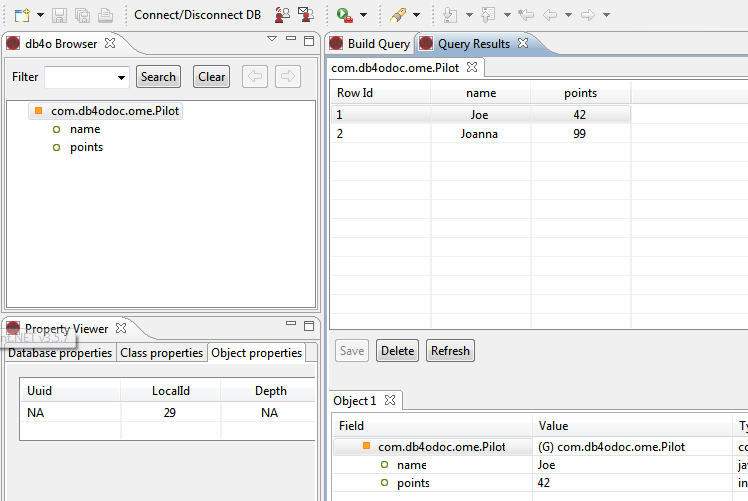
\includegraphics[width=\maxwidth]{images/ref-object-manager-enterprise-ome-for-eclipse-ome1.png}
\end{center}
In the OME perspective you can see:

\begin{itemize}
\item OME menu:

\begin{center}
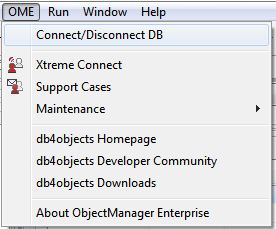
\includegraphics[width=\maxwidth]{images/ref-object-manager-enterprise-ome-for-eclipse-ome-menu.png}
\end{center}
\item OME toolbar buttons to access the frequently used functionality fast
\item Db4o Browser: window displaying the contents of the open db4o database
\item Property Viewer: window displaying the properties of the open database or the properties of the selected database class
\item Build Query: windows allowing to build a query using drag\&drop functionality
\item Query Results: window to browse the results of the query execution
\end{itemize}

\section{Browsing a Database}
\label{ref:object-manager-enterprise-ome-for-eclipse-browsing-a-database}

Suppose you have a simple database file containing Pilot and Car objects. Please select OME-\textgreater{}Connect/Disconnect DB (or use a shortcut button from the toolbar menu) and browse to your database file.

Once you've connected you will see a screen similar to this:

\begin{center}
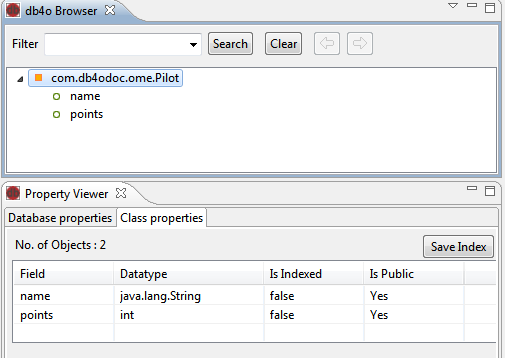
\includegraphics[width=\maxwidth]{images/ref-object-manager-enterprise-ome-for-eclipse-ome-pilot.png}
\end{center}
The db4o Browser window in the picture above shows that there is 1 class in the database (Pilot), which contains 2 fields: name and points. In the Property Viewer you can see more information about the class fields. You can also change "Is indexed" field and add the index to the database by pressing "Save Index" button.

The filter panel on the top of the view allows easier navigation through the database with lots of different classes. You can use wildcard searches and benefit from the search history to make the selection faster.

\section{Querying}
\label{ref:object-manager-enterprise-ome-for-eclipse-querying}

It is easy to retrieve all of the Pilot instances from the database: just right-click the Pilot class in db4o Browser and select "View All Objects". The list of the Pilot objects will be shown in the Query Result view:

\begin{center}
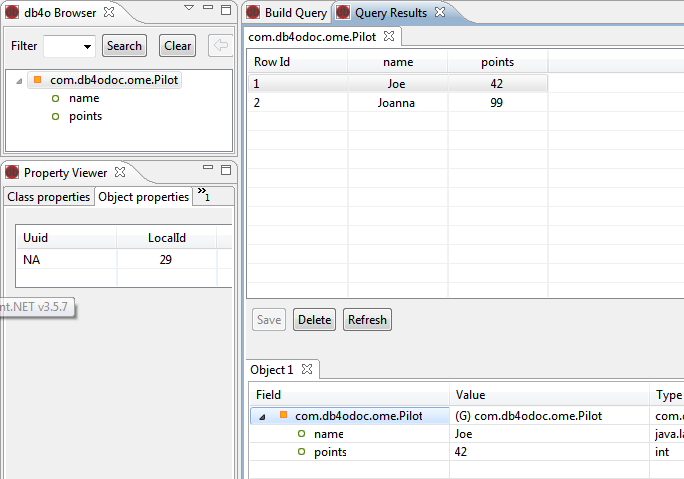
\includegraphics[width=\maxwidth]{images/ref-object-manager-enterprise-ome-for-eclipse-ome-result.png}
\end{center}
You can see object details in the detailed view below. Try to change any values and use Save button to persist the changes to the database. You can also use Delete button to delete objects from the database. For the objects containing field objects you will be prompted to use cascade on delete.

More complex queries can be done by using Build Query view:

\begin{center}
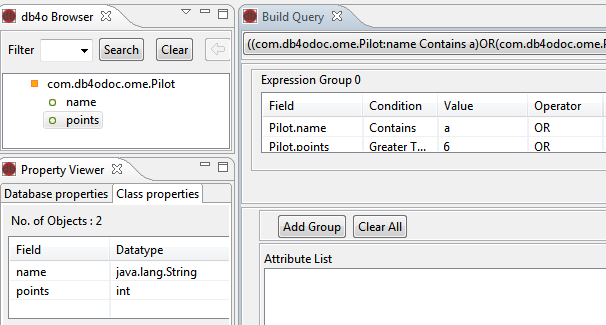
\includegraphics[width=\maxwidth]{images/ref-object-manager-enterprise-ome-for-eclipse-ome-query.png}
\end{center}
Drag "points" field from the db4oBrowser view into the Build Query view, set condition "Greater Than", put a value "99" and run the query. You can return to the Built Query tab and modify the query later on again. For example: add "AND" operator, drag "name" field and set the value to "Michael Schumacher". Re-run the query.

When the new query is created, the previous query is stored and can be selected from the history drop-down:

\begin{center}
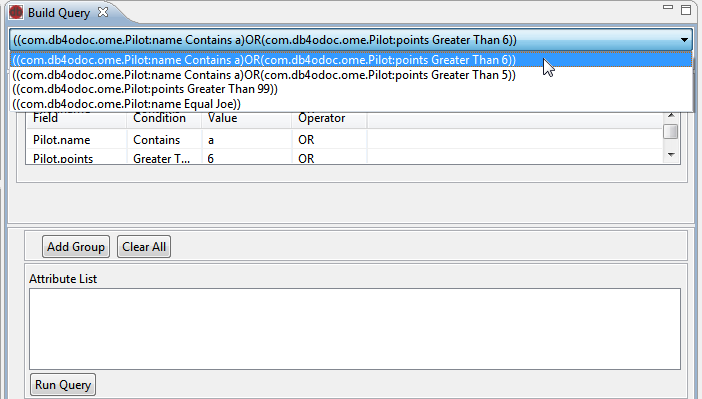
\includegraphics[width=\maxwidth]{images/ref-object-manager-enterprise-ome-for-eclipse-ome-qhistory.png}
\end{center}
More sophisticated queries can be build by joining grouped constraints using "Add Group" button.

When you are done working with the database in OME, you can close the connection by using OME-\textgreater{}Connect/Disconnect DB menu command or by using the equivalent button on the toolbar.

\section{Custom Configuration}
\label{ref:object-manager-enterprise-ome-for-eclipse-custom-config}

When the database cannot be opened with OMJ you should try to pass your configuration to OMJ. This ensures that OMJ opens the database the same way as your application does.

\subsection*{Prepare Configuration Jar File}

First you need to prepare a jar-file which contains code to configure OMJ. You do this by implementing the EmbeddedConfigurationItem-interface or implementing ClientConfigurationItem-interface.

In the implementation you can apply all the configuration settings to the object container which you use in your application.

\begin{lstlisting}
public class ConfigureDBForOmj implements EmbeddedConfigurationItem{
    public void prepare(EmbeddedConfiguration embeddedConfiguration) {
        // Your configuration goes here.
        // For example:
        embeddedConfiguration.common().add(new UuidSupport());
    }

    public void apply(EmbeddedObjectContainer embeddedObjectContainer) {
    }
}
\end{lstlisting}

{\small\itshape ConfigureDBForOmj.java: A configuration item for Java\par}
\medskip

Then create the file 'com.db4o.config.EmbeddedConfigurationItem' in the 'META-INF/services' folder of your jar. Add the fully qualified name of your EmbeddedConfigurationItem/ClientConfigurationItem-implementation. You can list as many implementations as you want.

\begin{lstlisting}
com.db4odoc.omj.ConfigureDBForOmj
\end{lstlisting}

{\small\itshape com.db4o.config.EmbeddedConfigurationItem: List all configuration items for OMJ\par}
\medskip

Finally you need to package the compiled code and the 'META-INF/service' folder into a jar-file. The jar-layout should be like this:

\begin{center}
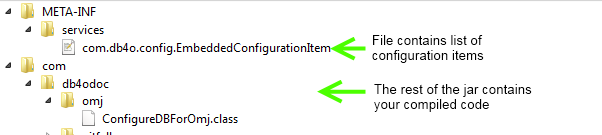
\includegraphics[width=\maxwidth]{images/ref-object-manager-enterprise-ome-for-eclipse-jar-overview.png}
\end{center}
\subsection*{Using the Configuration in OMJ}

After that you can choose the 'Custom config...' option on the open-dialog. There add the jar-file you've build previously. On the right all configuration-items are listed. Select the appropriate configuration items for your database.

\begin{center}
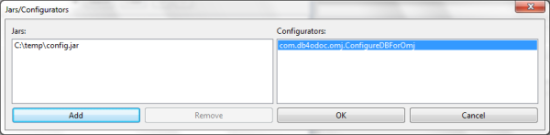
\includegraphics[width=\maxwidth]{images/ref-object-manager-enterprise-ome-for-eclipse-custom-config.png}
\end{center}
\section{Problems?}
\label{ref:object-manager-enterprise-ome-for-eclipse-problems}

Are you experiencing problems with the object manager? You can take a look at the error log in the Eclipse workspace. The log is located here: "workspace/.metadata/.log". Maybe you need to first clean up the log and then reproduce the issue.

When you are using advanced configuration features like type handlers, special string encoding etc. you should \hyperref[ref:object-manager-enterprise-ome-for-eclipse-custom-config]{add your configuration} (p.~\pageref{ref:object-manager-enterprise-ome-for-eclipse-custom-config}) to the object manager.

Otherwise ask for help in the \href{http://community.versant.com/Forums.aspx}{db4o forums}. When you see errors in the log please include them in your post.


% Converted from reference/DB4OFlare (MadCap Flare, Java target)

\chapter{Community}
\label{ref:community}

Participate in the db4o community and help to improve db4o. The main community website for db4o is \href{http://community.versant.com/}{http://community.versant.com/}. There you can find the db4o forums, blog posts additional resources and the newest db4o releases.

\section{Forums}
\label{ref:community:db4o}

The best place to ask questions about db4o, discuss and make suggestions are the db4o forums. You can find the db4o forums here:\href{http://community.versant.com/Forums.aspx}{http://community.versant.com/Forums.aspx}

\section{Resources \& News}
\label{ref:community:addition}

To stay informed about new features, community activity and other news subscribe to the different db4o blogs: \href{http://community.versant.com/Blogs.aspx}{http://community.versant.com/Blogs.aspx}

Or follow us on Twitter: \href{http://twitter.com/db4objects}{http://twitter.com/db4objects}

\section*{Report Bugs}

Every software contains bugs and so does db4o. If you find bugs please report them to us. In case you're not sure if you really found a bug, you maybe want to discuss your issue first on the \href{http://community.versant.com/Forums.aspx}{db4o forum}. As soon as you're sure that you found a bug it best to report in \href{http://tracker.db4o.com/}{our bug-tracking system}. The login is the same as in the db4o forums. Read more on tips and tricks for reporting bugs \hyperref[ref:community-report-bugs]{here} (p.~\pageref{ref:community-report-bugs}).

When possible include a small test program which reproduces the issue with the bug report. A test case avoids confusion and effort to reproduce the bug.

\section*{Working with the Source Code}

\hyperref[ref:community-working-with-source-code]{See "Working With Source Code"} (p.~\pageref{ref:community-working-with-source-code})

\section{Report Bugs}
\label{ref:community-report-bugs}

Found a bug in db4o? Here are a few tips and tricks for reporting bugs.

\subsection*{Where Do I Report Bugs?}

The best way to report a bug is to report it on our issue \href{http://tracker.db4o.com/}{tracking system}. The login for the bug tracker is the same as in the db4o community page and db4o forums. If you don't have a login yet you can register \href{http://community.versant.com/register.aspx}{here}.

In cases you are not sure if the issue is an bug or another problem you maybe want to discuss it in the \href{http://community.versant.com/register.aspx}{db4o forums}.

\subsection*{What Should the Bug Report Contain?}

The bug report should be as specific as possible, so that the room for interpretation is very small:

\begin{itemize}
\item Steps to reproduce the bug. In order to fix the bug a step by step instruction on how to reproduce the issue is essential.
\item When possible include a the test-code which reproduces the issue.
\item Include the db4o version in your bug report. The complete version of db4o is included in the jar-name.
\item Include information about your platform. Which Java Version and what kind of device (like Android).  Which .NET version and what kind of device (for example a embedded system)
\item In case of exceptions, please add also the stack trace.
\end{itemize}

\section{Working With Source Code}
\label{ref:community-working-with-source-code}

db4o is an open-source project. The source is available for reviewing, modifying for own needs or contributing your modifications. You can use the \hyperref[ref:community-working-with-source-using-the-sources-from-db4o-distribution]{source code from the downloaded distribution} (p.~\pageref{ref:community-working-with-source-using-the-sources-from-db4o-distribution}) package or you may use our \hyperref[ref:community-working-with-source-using-the-repository]{SVN repository} (p.~\pageref{ref:community-working-with-source-using-the-repository}) to get the latest modifications.

More Reading:

\begin{itemize}
\item \hyperref[ref:community-working-with-source-db4o-testing-framework]{Unit Tests for db4o} (p.~\pageref{ref:community-working-with-source-db4o-testing-framework})
\item \hyperref[ref:community-working-with-source-sharpen]{Sharpen: Converting Java to C\#} (p.~\pageref{ref:community-working-with-source-sharpen})
\item \hyperref[ref:community-working-with-source-using-the-sources-from-db4o-distribution]{Using The Sources From db4o Distribution} (p.~\pageref{ref:community-working-with-source-using-the-sources-from-db4o-distribution})
\item \hyperref[ref:community-working-with-source-using-the-repository]{Using The Repository} (p.~\pageref{ref:community-working-with-source-using-the-repository})
\item \hyperref[ref:community-working-with-source-building-full-distribution]{Building Full Distribution} (p.~\pageref{ref:community-working-with-source-building-full-distribution})
\item Building Java Version
\item \hyperref[ref:community-working-with-source-patch-submission]{Patch Submission} (p.~\pageref{ref:community-working-with-source-patch-submission})
\end{itemize}

\subsection{Sharpen}
\label{ref:community-working-with-source-sharpen}

Sharpen is an tool that allows you to convert your Java db4o project into C\#. The difference between sharpen and other java-to-C\# converters is the native support for db4o, .NET naming conventions and customization options.

More Reading:

\begin{itemize}
\item \hyperref[ref:community-working-with-source-sharpen-how-to-setup-sharpen]{How To Setup Sharpen} (p.~\pageref{ref:community-working-with-source-sharpen-how-to-setup-sharpen})
\item \hyperref[ref:community-working-with-source-sharpen-example-conversion]{Doing a Sharpen Conversion} (p.~\pageref{ref:community-working-with-source-sharpen-example-conversion})
\item \hyperref[ref:community-working-with-source-sharpen-sharpen-command-line-arguments]{Sharpen Command-Line Arguments} (p.~\pageref{ref:community-working-with-source-sharpen-sharpen-command-line-arguments})
\item \hyperref[ref:community-working-with-source-sharpen-sharpen-annotations]{Sharpen Annotations} (p.~\pageref{ref:community-working-with-source-sharpen-sharpen-annotations})
\end{itemize}

\subsubsection{How To Setup Sharpen}
\label{ref:community-working-with-source-sharpen-how-to-setup-sharpen}

You can obtain sharpen source from db4o svn repository at:

\href{https://source.db4o.com/db4o/trunk/sharpen}{https://source.db4o.com/db4o/trunk/sharpen}

For the ease of use check-out sharpen projects:

\begin{itemize}
\item sharpen.builder
\item sharpen.core
\item sharpen.ui
\item sharpen.ui.tests
\end{itemize}

Additionally Sharpen requires a valid \href{http://eclipse.org/}{Eclipse} installation to run. Install Eclipse on your machine or reuse an existing installation. Check out the four projects into the same workspace as your java project which you want to convert. This is not required is easier to use and maintain.

The first step is to build sharpen. For that we can use Apache Ant:

\begin{lstlisting}
<target name="build-sharpen">
    <property name="sharpen.core.dir" location="${dir.workspace}/sharpen.core"/>
    <reset-dir dir="${dir.dist.classes.sharp}"/>

    <javac fork="true"
           debug="true"
           target="1.5"
           source="1.5"
           destdir="${dir.dist.classes.sharp}"
           srcdir="${sharpen.core.dir}/src"
           encoding="UTF-8">
        <classpath>
            <fileset dir="${eclipse.home}/plugins">
                <include name="org.eclipse.osgi_*.jar"/>
                <include name="org.eclipse.core.resources_*.jar"/>
                <include name="org.eclipse.core.runtime_*.jar"/>
                <include name="org.eclipse.jdt.core_*.jar"/>
                <include name="org.eclipse.jdt.launching_*.jar"/>
                <include name="org.eclipse.equinox.*.jar"/>
                <include name="org.eclipse.core.jobs_*.jar"/>
            </fileset>
        </classpath>
    </javac>
    <jar destfile="${dir.dist.classes.sharp}/sharpen.core_1.0.0.jar" basedir="${dir.dist.classes.sharp}">
        <fileset dir="${sharpen.core.dir}">
            <include name="plugin.xml"/>
        </fileset>
    </jar>
</target>
\end{lstlisting}

{\small\itshape sharpen-install.xml: Build Sharpen\par}
\medskip

To run Sharpen you should install it to an Eclipse instance:

\begin{lstlisting}
<target name="install-sharpen-plugin" depends="build-sharpen">
    <copyfile src="${dir.dist.classes.sharp}/sharpen.core_1.0.0.jar" dest="${plugins.home}/sharpen.core_1.0.0.jar"/>
</target>
\end{lstlisting}

{\small\itshape sharpen-install.xml: Install Sharpen to Eclipse\par}
\medskip

Put the paths for the build in a property file, so that you can easily change them. Here's a example of the property file. You have to configure the JDK-path, the Eclipse path and the path to the Sharpen source.

\begin{lstlisting}
#The workspace where the sharpen projects are
dir.workspace=C:/Users/Gamlor/Develop/db4o/sharpenProject
# Java executable
jdk.home=${env.JAVA_HOME}
jdk.home.java=${jdk.home}/bin/java.exe
# Eclipse home directory
eclipse.home=C:/progs/eclipse
# Sandcastle can be used to convert javadoc to .NET xml comments
# dir.lib.sandcastle=e:/sandcastle/
# sharpen compile directory
dir.dist.classes.sharp=${dir.workspace}/dist/
# Eclipse plugins home
plugins.home=${eclipse.home}/plugins
\end{lstlisting}

{\small\itshape sharpen.properties: The configuration for building sharpen\par}
\medskip

After that Sharpen is set up to run.

\subsubsection{Doing a Sharpen Conversion}
\label{ref:community-working-with-source-sharpen-example-conversion}

Ensure that you've installed sharpen to an existing eclipse installation as explained \hyperref[ref:community-working-with-source-sharpen-how-to-setup-sharpen]{here} (p.~\pageref{ref:community-working-with-source-sharpen-how-to-setup-sharpen}).

Use Ant scripts to run Sharpen and translate your Java code to C\#. The best way for this is to define an Ant macro which you then can reuse. This task takes two arguments. The first argument is the path to a valid Eclipse workspace which contains the project to translate. The second parameter is the project in the workspace which you want to translate.

\begin{lstlisting}
<macrodef name="sharpen">
    <attribute name="workspace"/>
    <attribute name="resource"/>

    <element name="args" optional="yes"/>

    <sequential>
        <java taskname="sharpen"
              fork="true"
              classname="org.eclipse.core.launcher.Main"
              failonerror="true" timeout="1800000">

            <classpath>
                <fileset dir="${eclipse.home}/plugins">
                    <include name="org.eclipse.equinox.launcher_*.jar"/>
                </fileset>
            </classpath>

            <arg value="-clean"/>
            <arg value="-data"/>
            <arg file="@{workspace}"/>
            <arg value="-application"/>
            <arg value="sharpen.core.application"/>
            <arg value="@{resource}"/>
            <args/>
        </java>
    </sequential>
</macrodef>
\end{lstlisting}

{\small\itshape sharpen-install.xml: The sharpen task\par}
\medskip

Now you can use this task to sharpen your project. First ensure that your project is in a valid Eclipse workspace. Then you specify the workspace and the sources of the project:

\begin{lstlisting}
<target name="sharpen">
    <sharpen
        workspace="C:\temp\sharpenExamples\"
        resource="example/src">
        <args>
            <arg value="@sharpen-config"/>
        </args>
        </sharpen>
</target>
\end{lstlisting}

{\small\itshape sharpen-example.xml: Sharpen a example project\par}
\medskip

Additionally you can pass the sharpen configuration as a file-name. When you add a '@' in front of the file-name sharpen will read that file and use all configuration flags of that. For example:

\begin{lstlisting}
-pascalCase+
-nativeTypeSystem
-nativeInterfaces
\end{lstlisting}

You can find a list of all Sharpen \hyperref[ref:community-working-with-source-sharpen-sharpen-command-line-arguments]{configuration flags here} (p.~\pageref{ref:community-working-with-source-sharpen-sharpen-command-line-arguments}) and a list of all \hyperref[ref:community-working-with-source-sharpen-sharpen-annotations]{Sharpen annotations here} (p.~\pageref{ref:community-working-with-source-sharpen-sharpen-annotations}).

\subsubsection{Sharpen Command-Line Arguments}
\label{ref:community-working-with-source-sharpen-sharpen-command-line-arguments}

Sharpen command-line arguments can be defined in an options file

\begin{lstlisting}
<sharpen workspace="${target.dir}" resource="sharpened_examples/src">
   <args>
      <!-- Sharpen options are defined in a separate file -->
      <arg value="@sharpen-all-options" />
    </args>
 </sharpen>      
\end{lstlisting}

Here sharpen-all-options file contains all command-line options needed to convert current project. For an example of command-line options file see the \hyperref[ref:community-working-with-source-sharpen-example-conversion]{previous topic} (p.~\pageref{ref:community-working-with-source-sharpen-example-conversion}).

Command-line arguments can also be specified directly in an ant script:

\begin{lstlisting}
<sharpen workspace="${dir.sharpen}" resource="db4oj/core/src">
    <args>
        <arg value="-xmldoc"/>
        <arg file="config/sharpen/ApiOverlay.xml" />       
        <arg value="@sharpen-all-options" />
     </args>
 </sharpen>
        
\end{lstlisting}

The following table shows available command-line options, their meaning and example usage:

{\small
\begin{longtable}{|p{\dimexpr(\linewidth-3\arrayrulewidth)*1/2-2\tabcolsep\relax}|p{\dimexpr(\linewidth-3\arrayrulewidth)*1/2-2\tabcolsep\relax}|}
\hline
\textbf{Argument} & \textbf{Usage} \\ \hline
-pascalCase & Convert Java identifiers to Pascal case \\ \hline
-pascalCase+ & Convert Java indentifiers and package names (namespaces) to Pascal case \\ \hline
-cp & Adds a new entry to classpath:\par \textless{}arg value="-cp" /\textgreater{}\par \textless{}arg path="lib/db4o-7.2.37.10417-java5.jar" /\textgreater{} \\ \hline
-srcFolder & Adds a new source folder for sharpening \\ \hline
-nativeTypeSystem & Map java classes to .NET classes with a similar functionality. For example: java.lang.Class - System.Type \\ \hline
-nativeInterfaces & Adds an "I" in front of the interface name \\ \hline
-organizeUsings & Adds "using" for the types used \\ \hline
-fullyQualify & Converts to a fully-qualified name:\par -fullyQualify File \\ \hline
-namespaceMapping & Maps a java package name to a .NET namespace. For example:\par -namespaceMapping com.db4o Db4objects.Db4o \\ \hline
-methodMapping & Maps a java method name to a .NET method (can be method in another class). For example:\par -methodMapping java.util.Date.getTime Sharpen.Runtime.ToJavaMilliseconds \\ \hline
-typeMapping & Maps a java class to .NET type:\par -typeMapping com.db4o.Db4o Db4objects.Db4o.Db4oFactory \\ \hline
-propertyMapping & Maps a java method to .NET property:\par -propertyMapping com.db4odoc.structured.Car.getPilot Pilot \\ \hline
-runtimeTypeName & Name of the runtime class. The runtime class provides implementation for methods that don't have a direct mapping or that are simpler to map at the language level than at the sharpen level. For instance: String.substring, String.valueOf, Exception.printStackTrace, etc.\par For a complete list of all the method that can be mapped to the runtime class see Configuration\#runtimeMethod call hierarchy. \\ \hline
-header & Header comment to be added to all converted files.\par -header config/copyright\_comment.txt \\ \hline
-xmldoc & Specifies an xml-overlay file, which overrides javadoc documentation for specific classes:\par -xmldoc config/sharpen/ApiOverlay.xml \\ \hline
-eventMapping & Converts the methods to an event. \\ \hline
-eventAddMapping & Marks the method as an event subscription method. Invocations to the method in the form \textless{}target\textgreater{}.method(\textless{}argument\textgreater{}) will be replaced by the c\# event subscription idiom: \textless{}target\textgreater{} += \textless{}argument\textgreater{} \\ \hline
-conditionalCompilation & Add a condition when to translate the Java code\par - -conditionalCompilation com.db4o.db4ounit.common.cs !SILVERLIGHT \\ \hline
-configurationClass & Change the configuration class. The default is 'sharpen.core.DefaultConfiguration' \\ \hline
\end{longtable}}

\subsubsection{Sharpen Annotations}
\label{ref:community-working-with-source-sharpen-sharpen-annotations}

Sharpen annotations decorate java source code and are used to notify sharpener about how the code should be processed and converted. Annotations can be used to specify how a code element should be converted (for example class to enum), to skip conversion of some code elements, to rename classes, to change visibility etc.

The following table shows existing annotations, their meaning and examples.

{\small
\begin{longtable}{|p{\dimexpr(\linewidth-3\arrayrulewidth)*1/2-2\tabcolsep\relax}|p{\dimexpr(\linewidth-3\arrayrulewidth)*1/2-2\tabcolsep\relax}|}
\hline
\textbf{Annotation} & \textbf{Meaning} \\ \hline
@sharpen.enum & Mark java class to be processed as a .NET enum \\ \hline
@sharpen.rename & Specifies a different name for the converted type, takes a single name argument. For example:\par @sharpen.rename Db4oFactory \\ \hline
@sharpen.private & Specifies that the element must be declared private in the converted file, though it can be not private in the java source:\par \begin{lstlisting}
/*
* @sharpen.private
*/
\end{lstlisting}\par public List4 \_first; \\ \hline
@sharpen.internal & Specifies that the element must be declared internal in the converted file:\par \begin{lstlisting}
/**
 * @sharpen.internal
*/
\end{lstlisting}\par public abstract int size(); \\ \hline
@sharpen.protected & Specifies that the element must be declared protected in the converted file:\par \begin{lstlisting}
/**
 * @sharpen.protected
*/
\end{lstlisting}\par public abstract int size(); \\ \hline
@sharpen.new & Adds the C\#-'new' modifier to the translated code. \\ \hline
@sharpen.event & Links an event to its arguments. For example:\par Java:\par \begin{lstlisting}
/**
* @sharpen.event com.db4o.events.QueryEventArgs
*/
public Event4 queryStarted();
\end{lstlisting}\par is converted to:\par \begin{lstlisting}
public delegate void QueryEventHandler(
  object sender,
  Db4objects.Db4o.Events.QueryEventArgs args);
.......
event Db4objects.Db4o.Events.QueryEventHandler QueryStarted;
\end{lstlisting} \\ \hline
@sharpen.event.add & Marks the method as an event subscription method. Invocations to the method in the form \textless{}target\textgreater{}.method(\textless{}argument\textgreater{}) will be replaced by the c\# event subscription idiom: \textless{}target\textgreater{} += \textless{}argument\textgreater{} \\ \hline
@sharpen.event.onAdd & Valid for event declaration only (SHARPEN\_EVENT). Configures the method to be invoked whenever a new event handler is subscribed to the event. \\ \hline
@sharpen.if & Add \#if \textless{}expression\textgreater{}\#endif declaration:\par @sharpen.if \textless{}expression\textgreater{} \\ \hline
@sharpen.property & Convert a java method as a property:\par \begin{lstlisting}
/**
 * @sharpen.property
*/
\end{lstlisting}\par public abstract int size(); \\ \hline
@sharpen.indexer & Marks an element as an indexer property \\ \hline
@sharpen.ignore & Skip the element while converting \\ \hline
@sharpen.ignore.extends & Ignore the extends clause in Java class definition \\ \hline
@sharpen.ignore.implements & Ignore the implements clause in Java class definition \\ \hline
@sharpen.extends & Adds an extends clause to the converted class definition. For example:\par Java:\par \begin{lstlisting}
/**
* @sharpen.extends System.Collections.IList
*/
public interface ObjectSet {...
\end{lstlisting}\par converts to\par \begin{lstlisting}
public interface IObjectSet : System.Collections.IList
\end{lstlisting} \\ \hline
@sharpen.partial & Marks the converted class as partial \\ \hline
@sharpen.remove & Marks a method invocation that should be removed \\ \hline
@sharpen.remove.first & Removes the first line of the method/constructor when converting to C\#:\par \begin{lstlisting}
/**
* @sharpen.remove.first
*/
public void doSomething(){
    System.out.println("Java");
    NextMethod();
}
\end{lstlisting}\par converts to:\par \begin{lstlisting}
public void DoSomething(){
    NextMethod();
}
\end{lstlisting} \\ \hline
@sharpen.struct & Marks class to be converted as c\# struct \\ \hline
@sharpen.unwrap & When a method is marked with this annotation \newline{}all method calls are removed. This is useful for removing conversion methods when their aren't required in C\#.\par \begin{lstlisting}
/*
* @sharpen.unwrap
*/
public Iterable toIterable(Object[] array){
   return Arrays.asList(array);
}
public void doSomething(Object[] objs){
  Iterable iterable = toIterable(objs);
  // do something with the iterable
}
\end{lstlisting}\par Is converted to:\par \begin{lstlisting}
public IEnumerable ToIterable(object[] array){
    return Arrays.AsList(array);
}
public void doSomething(object[] objs){
   Iterable iterable = objs;
   // do something with the iterable
}
\end{lstlisting} \\ \hline
@sharpen.attribute & Adds an attribute to the converted code:\par \begin{lstlisting}
/*
* @sharpen.attribute TheAttribute
*/
public void doSomething(){}
\end{lstlisting}\par Will be converted to:\par \begin{lstlisting}
[TheAttribute]
public void DoSomething(){}
\end{lstlisting} \\ \hline
@sharpen.macro & Add a replace-pattern macro to your code. \\ \hline
\end{longtable}}

\subsection{db4o Testing Framework}
\label{ref:community-working-with-source-db4o-testing-framework}

db4ounit is a minimal xUnit (jUnit, NUnit) style testing framework. The db4ounit framework was created to fulfill the following requirements:

\begin{itemize}
\item The core tests should be run against JDK1.1
\item It should be possible to automatically convert test cases from Java to .NET.
\end{itemize}

db4ounit design deviates from vanilla xUnit in some respect, but if you know xUnit, db4ounit should look very familiar.

db4ounit itself is completely agnostic of db4o, but there is the db4ounit.extensions module which provides a base class for db4o specific test cases with different fixtures, etc.

Db4ounit and db4ounit.extensions are supplied as a source code for both java and .NET. Java version also comes with a compiled library: db4o-X.XX-db4ounit.jar, which allows you to run your tests from a separate package.

If you've found a bug and want to supply a test case to help db4o to fix the issue quickly, the best option would be to supply your code in the java db4ounit format. This format allows very easy integration of a new test case into db4o test suite: only copy/paste is required to put your test class code into the framework using Eclipse.

More Reading:

\begin{itemize}
\item \hyperref[ref:community-working-with-source-db4o-testing-framework-creating-a-sample-test]{Creating A Sample Test} (p.~\pageref{ref:community-working-with-source-db4o-testing-framework-creating-a-sample-test})
\item \hyperref[ref:community-working-with-source-db4o-testing-framework-db4ounit-methods]{Db4ounit Methods} (p.~\pageref{ref:community-working-with-source-db4o-testing-framework-db4ounit-methods})
\end{itemize}

\subsubsection{Creating A Sample Test}
\label{ref:community-working-with-source-db4o-testing-framework-creating-a-sample-test}

Let's create the a extremely simple test case. The first step is to setup db4ounit. The best way is to use db4ounit directly from the source. db4ounit is in the db4o source code folder of the distribution.

Open the db4o source-code of the db4o test-projects in Eclipse (or another IDE). The db4ounit projects are called 'db4ounit' and 'db4ounit.extensions'. Then create a new project which references the db4ounit projects.

After that we're ready to write our first db4ounit test. Create a new class which inherits from AbstractDb4oTestCase. Then add a test-method. Any method which starts with the prefix 'test' is a test method. Then add a main method which starts the test.

\begin{lstlisting}
public class ExampleTestCase extends AbstractDb4oTestCase{

    public static void main(String[] args) {
        new ExampleTestCase().runEmbedded();
    }

    public void testStoresElement(){
        db().store(new TestItem());
        ObjectSet<TestItem> result = db().query(TestItem.class);
        Assert.areEqual(1, result.size());
    }

    static class TestItem{

    }
}
\end{lstlisting}

{\small\itshape ExampleTestCase.java: Basic test case\par}
\medskip

\subsubsection{db4ounit Methods}
\label{ref:community-working-with-source-db4o-testing-framework-db4ounit-methods}

Let's look through the basic API , which will help you to build your own test. This document is not a complete API reference and its intention is to give you a general idea of the methods usage and availability.

\paragraph*{AbstractDb4oTestCase}

AbstractDb4oTestCase is a base class for creating test cases. It will setup a db4o instance for you which you can use in your tests. Additionally it provides different utility methods for configuring, querying and modifying the database.

Additionally it contains methods to run the test. You can create new instance of a class which extends AbstractDb4oTestCase and run the test in different environments. For example the method 'runSolo' will run the test with an embedded local container.

\paragraph*{TestCase}

This interface provides the basic for a unit test in the db4ounit framework. When you implement this interface the class is a valid unit test. All methods starting with 'test' will be executed as test.

For most tests it is more continent to use the AbstractDb4oTestCase.

\paragraph*{TestLifeCycle}

This interface provides a test case with additional setup and tear down methods. Those will be called before and after each test method

\paragraph*{ConsoleTestRunner}

A test-runner which runs the tests as console application.

Usually it's more convenient to extend the AbstractDb4oTestCase class and use the provided run methods instead of the console test runner.

\paragraph*{Db4ounit.Assert}

This class provides a variety of methods for asserting certain conditions

\subsection{Using The Sources From db4o Distribution}
\label{ref:community-working-with-source-using-the-sources-from-db4o-distribution}

The sources for db4o are in the 'src' subdirectory of the db4o distribution. You simply can open these projects in Eclipse (or another IDE). Compile and use the db4o projects like any other Eclipse project.

Following projects are shipped with db4o:

\begin{itemize}
\item bloat: The bytecode manipulation library used by db4o.
\item db4o.cs: The db4o client server mode.
\item db4o.cs.optional: Optional additions for the db4o client server mode.
\item db4o.instrumentation: The base for different instrumentations provided by db4o.
\item db4o\_osgi: The db4o OSGi service
\item db4o\_osgi\_test: The test cases for the db4o OSGi service.
\item db4oj: The db4o core.
\item db4oj.optional: Optional features for db4o.
\item db4oj.tests: The db4o test-suite.
\item db4onqopt: The db4o native query optimization.
\item db4otaj: Transparent activation/persistence enhancers.
\item db4otools: Tooling for db4o like Ant-tasks
\item db4ounit: The db4o unit test framework.
\item db4ounit.extensions: Utilities and extensions for the db4o unit test framework.
\end{itemize}

\subsection{Using The Repository}
\label{ref:community-working-with-source-using-the-repository}

If you enjoy being on the "cutting edge" and want to follow up with the development process, you can use our SVN repository to get the most up-to-date db4o source code.

Access to the public projects on our Subversion server is available under the following public URL. No login is required.

\href{https://source.db4o.com/db4o/trunk/}{https://source.db4o.com/db4o/trunk/}

The following projects are currently available.

Projects may be under constant development. Source code is not guaranteed to be stable.

Most top-level modules in svn directly map to Eclipse projects, i.e. the root folder contains the Eclipse project metadata.

\begin{itemize}
\item bloat: The byte code manipulation library db4o uses.
\item db4o.cs: The client server implementation for db4o.
\item db4o.cs.optional: Optional client server features for db4o.
\item db4o.instrumentation: The instrumentation basic functionality for db4o.
\item db4o.net: The .NET version of db4o.
\item db4obuild: The build scripts for db4o.
\item db4onqopt: The db4o native query optimizer.
\item db4otaj: The db4o transparent activation/persistence enhancer.
\item db4otools: The db4o tools like Ant scripts.
\item db4ounit: The db4o test project.
\item db4ounit.extensions: Additional unit test functionality.
\item decaf: The Java 1.5 to Java 1.4 converter. You need to checkout all sub-projects on the same level as other db4o projects.
\item drs: The db4o replication system.
\item sharpen: The Java to C\# converter. You need to checkout all sub-projects on the same level as other db4o projects.
\end{itemize}

\subsection{Building Full Distribution}
\label{ref:community-working-with-source-building-full-distribution}

Building full distribution will allow you to get the same db4o packages as you can get from db4o download center. However, the flexibility of the build project also allows you to get only parts of it, like only java distro, only documentation, only tests etc.

The following documentation explains how to build a full distribution using Eclipse version 3.4 Ganymede. It is assumed that you have \href{http://ant.apache.org/}{ant} and one of Eclipse SVN clients (\href{http://subclipse.tigris.org/}{Subclipse} or \href{http://www.eclipse.org/subversive/}{Subversive}) installed.

\subsubsection*{Projects Required}

In order to build db4o you will need to check out the following projects.

\begin{itemize}
\item bloat: The byte code manipulation library db4o uses.
\item db4o.cs: The client server implementation for db4o.
\item db4o.cs.optional: Optional client server features for db4o.
\item db4o.instrumentation: The instrumentation basic functionality for db4o.
\item db4o.net: The .NET version of db4o.
\item db4obuild: The build scripts for db4o.
\item db4onqopt: The db4o native query optimizer.
\item db4otaj: The db4o transparent activation/persistence enhancer.
\item db4otools: The db4o tools like Ant scripts.
\item db4ounit: The db4o test project.
\item db4ounit.extensions: Additional unit test functionality.
\item decaf: The Java 1.5 to Java 1.4 converter. You need to checkout all sub-projects on the same level as other db4o projects.
\item drs: The db4o replication system.
\item sharpen: The Java to C\# converter. You need to checkout all sub-projects on the same level as other db4o projects.
\item doctor: A tool for building the tutorial.
\item tutorial: The db4o tutorial
\end{itemize}

\paragraph*{machine.properties}

You will need to create machine.properties file in db4obuild folder. The contents of the file can be copied from build.xml (see the comments at the beginning of the file). Modify the paths where applicable to set the build variables for your environment.

Read the instructions at top of the build.xml to find out what options are available. Here's an example:

\begin{lstlisting}
file.compiler.jdk1.3=%JAVA_HOME%/bin/javac.exe
file.compiler.jdk1.3.args.optional=-source 1.3
file.jvm.jdk1.5=%JAVA_HOME%/bin/java.exe
dir.workspace=C:/Users/Gamlor/Develop/db4o/db4o-src/
eclipse.home=C:/progs/eclipse
msbuild.executable="C:/Windows/Microsoft.NET/Framework/v4.0.30319/MSBuild.exe" 
\end{lstlisting}

\subsubsection*{Build Preparation}

First you will need to run some preparation scripts. This is done only once per workspace and should not be repeated in the future.

Run build-db4obuild.xml, this will compile some of the tools used in the build process.

You will need to generate a key to sign the tutorial applet. Use the following commands:

keytool -genkey -alias db4objects -keyalg rsa

keytool -export -alias db4objects -file [path]/db4obuild/config/db4objects.crt

Use "kistoa" (without quotes) as your keypass and storepass.

Replace [path] with the path to db4obuild project on your system and make sure that db4objects.crt file is created in db4obuild/config folder.

If you've already generated db4objects key pair before, you will need to delete it before re-generating:

keytool -delete -alias db4objects

You will need to add ant-contrib.jar to your eclipse ant. You can download ant-contib.jar at:

\href{http://sourceforge.net/projects/ant-contrib/}{http://sourceforge.net/projects/ant-contrib}

\begin{itemize}
\item Add ant-contib jar to ant folder in eclipse/plugins.
\item After this is done go to Window-\textgreater{}Preferences menu in Eclipse.
\item Select Ant-\textgreater{}Runtime in the list.
\item Then select "Ant Home Entries".
\item Press "Add External Jar" and select ant-contib.jar location in the plugins folder.
\end{itemize}

\subsubsection*{Running The Build}

Now everything is ready to run db4o build. Right-click build.xml file and select "Run As/Ant Build". You will need to run "buildall" target to generate java and .NET distribution.

\subsection{Patch Submission}
\label{ref:community-working-with-source-patch-submission}

This topic explains how to prepare your patch.

Before writing a patch, please, familiarize yourself with our Coding Style conventions.

You can create a patch using "Create Patch" SVN command.

If you are using \href{http://www.polarion.org/index.php?page=overview&project=subversive}{Subversive} plugin you can use the following steps:

\begin{itemize}
\item select the project in Package Explorer;
\item right-click and select Team/Create Patch;
\item select "Save In File System" and choose the file name;
\item click "Next" and "Finish";
\item check unversioned resources that should be included in the patch;
\item click "OK"
\end{itemize}

Once the patch is created you should register the functionality provided with our \href{http://tracker.db4o.com/secure/Dashboard.jspa}{Jira tracking system} by creating new issue, submitting the description, patch and \hyperref[ref:community-working-with-source-db4o-testing-framework]{test case} (p.~\pageref{ref:community-working-with-source-db4o-testing-framework}) if applicable.


% Converted from reference/DB4OFlare (MadCap Flare, Java target)

\chapter{Dependency Overview}
\label{ref:dependency-overview}

The different functionality of db4o is implemented in multiple jar s. You need to include only the jar which are required for you're application. Here's an overview:

\begin{center}
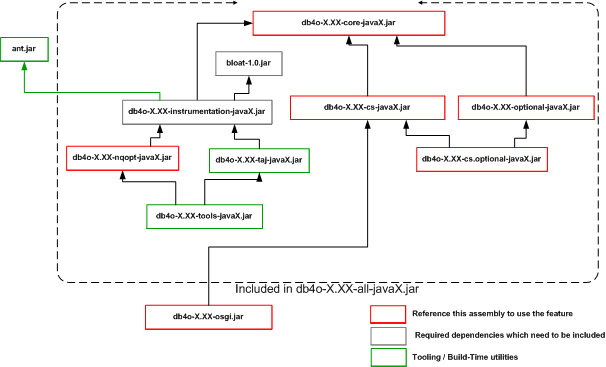
\includegraphics[width=\maxwidth]{images/ref-depedency-overview-java.png}
\end{center}
\section*{db4o-X.XX-core-javaX.jar}

This jar contains the \hyperref[ref:basics]{core functionality} (p.~\pageref{ref:basics}) of db4o. It doesn't have any dependencies to other jars.

\section*{db4o-X.XX-cs-javaX.jar}

This jar contains the \hyperref[ref:client-server]{client server mode} (p.~\pageref{ref:client-server}) of db4o. It only depends on the db4o-core jar.

\section*{db4o-X.XX-nqopt-javax.jar}

This jar contains the \hyperref[ref:basics-querying-native-queries]{native query optimizations} (p.~\pageref{ref:basics-querying-native-queries}) for db4o. Make sure that you include this jar when you use native queries. It depends on the db4o-core, db4o-instrumentation and the bloat jar for the runtime optimization.

When you use the \hyperref[ref:advanced-topics-enhancement-tools]{compile-time optimization} (p.~\pageref{ref:advanced-topics-enhancement-tools}) instead of the runtime optimization, it also requires the Ant library. However when you do compile-time optimization, you don't need this jar and its dependencies at runtime.

Note that the native queries work also without this jar in the classpath. However the queries cannot be optimized without this jar and will run a lot slower.

\section*{db4o-X.XX-optional-javaX.jar}

This jar contains some additional features and functionality for db4o, like \hyperref[ref:advanced-topics-runtime-statistics]{monitoring capabilities} (p.~\pageref{ref:advanced-topics-runtime-statistics}), \hyperref[ref:advanced-topics-type-handling-bigmath]{BigMath-support} (p.~\pageref{ref:advanced-topics-type-handling-bigmath}) and .NET support. It depends on the db4o-core jar.

\section*{db4o-X.XX-cs.optional-javaX.jar}

This jar contains additional features for the client-server-mode, like \hyperref[ref:client-server-pluggable-sockets-using-ssl-for-client-server-communication]{SSL} (p.~\pageref{ref:client-server-pluggable-sockets-using-ssl-for-client-server-communication}) and monitoring support. It depends on the db4o-cs, db4o-optional and the db4o-core jar.

\section*{db4o-X.XX-taj-javaX.jar}

This jar contains the utilities to enhance your classes with \hyperref[ref:advanced-topics-enhancement-tools]{transparent activation} (p.~\pageref{ref:advanced-topics-enhancement-tools}). It is normally used at compile time, but its possible to use it also at runtime. It depends on the db4o-core, db4o-instrumentation and the bloat-jar. Since the enhancement is usually done with Ant, it also requires the Ant-library.

\section*{db4o-X.XX-tools-javaX.jar}

This jar contains the \hyperref[ref:advanced-topics-enhancement-tools]{high level functionality for enhancing your classes} (p.~\pageref{ref:advanced-topics-enhancement-tools}). It requires the db4o-core, db4o-instrumentation, db4o-taj, db4o-nqopt and the bloat-jar. Additionally it needs the Ant-library.

\section*{db4o-X.XX-osgi.jar}

This jar contains a db4o OSGI service. It depends on the db4o-core and the db4o-cs jars.

\section*{db4o-X.XX-all-javaX.jar}

This jar contains all db4o functionality with all dependencies, except the Ant-library and the db4o-osgi library. If you just want to use db4o and aren't limited by space constrains use this jar only.


% Converted from reference/DB4OFlare (MadCap Flare, Java target)

\chapter{License}
\label{ref:license}

\section*{Licensing the db4o Engine}

db4o is free software, available under the \href{https://www.gnu.org/licenses/gpl-3.0.html}{GNU General Public License (GPL) version 3}. A copy of the license is in the LICENSE file of the \href{https://github.com/blakemcbride/db4o}{db4o repository}. Under the GPL, db4o can be used:

\begin{itemize}
\item for development
\item in-house as long as no deployment to third parties takes place
\item together with works that are placed under the GPL themselves
\end{itemize}

If you have questions whether the GPL is the right license for you, read the \href{https://www.gnu.org/licenses/gpl-faq.html}{GPL FAQ}.

Versant Corporation, the original developer, also offered db4o under a commercial license and under the db4o Opensource Compatibility License (dOCL) for open source projects under other licenses. Versant has discontinued db4o, and these licenses are no longer offered.

\section*{3rd Party Licenses}

The db4o source code includes the following 3rd party software:

\begin{itemize}
\item \href{https://ant.apache.org/}{Apache Ant} (Apache Software License)

Files: db4o.instrumentation/lib/ant.jar, ant-launcher.jar, ant.license.html

Ant is used for the enhancer's Ant tasks and can be used as a make tool for class file based optimization of native queries at compile time.

This product includes software developed by the Apache Software Foundation (\href{https://www.apache.org/}{\nolinkurl{https://www.apache.org/}}).
\item BLOAT (GNU LGPL), from Purdue University

Files: bloat/src, bloat/lgpl.license.txt; built into db4o-8.1-bloat.jar

BLOAT is used for bytecode analysis during native queries optimization. It needs to be on the classpath during runtime at load time or query execution time for just-in-time optimization. Preoptimized class files are not dependent on BLOAT at runtime.
\end{itemize}

These products are not part of db4o's licensed core and are licensed directly from their respective owners.

% Converted from reference/DB4OFlare (MadCap Flare, Java target)

\chapter{Contacts}
\label{ref:contacts}

\section*{Join The db4o Community}

Join the \href{http://community.versant.com/}{db4o community} for help, tips and tricks. Ask for help in the \href{http://community.versant.com/Forums.aspx}{db4o forums} at any time. If you want to stay informed, subscribe to \href{http://community.versant.com/Blogs.aspx}{db4o blogs}. \newline{}

\section*{Address and Contact Information}

\textbf{Versant Corporation}255 Shoreline Drive, Suite 450\newline{}Redwood City, CA 94065\newline{}USA

\textbf{Phone:}

+1 (650) 232-2436

\textbf{Fax:}

+1 (650) 232-2401

\textbf{Sales:}

Fill out our \href{http://www.db4o.com/commercial/purchase/enquiry.aspx}{sales contact form} on the db4o website or mail to \href{mailto:sales@db4o.com}{sales@db4o.com}

\textbf{Careers}

\href{mailto:career@db4o.com}{career@db4o.com}

\textbf{Partnering}

\href{mailto:partner@db4o.com}{partner@db4o.com}


\part{Replication (dRS)}
% Converted from reference/DRSFlare (MadCap Flare, Java target)

\chapter{db4o Replication System}
\label{drs:welcome}

The db4o Replication System provides functionality to periodically synchronize databases that work disconnected from each other. For example mobile devices synchronizing to a central server or desktop application.

The dRS can replicate between any number of db4o-databases. \hyperref[drs:db4o-replication-system-drs-db4o-databases-replication]{See "db4o to db4o Replication"} (p.~\pageref{drs:db4o-replication-system-drs-db4o-databases-replication})

Another feature is to replicate between VOD and db4o. \hyperref[drs:db4o-replication-system-drs-vod-replication]{See "Replication With VOD"} (p.~\pageref{drs:db4o-replication-system-drs-vod-replication})

Utilizing Hibernate dRS can also replicate between db4o and a RDBMS. \hyperref[drs:db4o-replication-system-drs-replication-with-rdbms]{See "Replication With Hibernate"} (p.~\pageref{drs:db4o-replication-system-drs-replication-with-rdbms})

\begin{center}
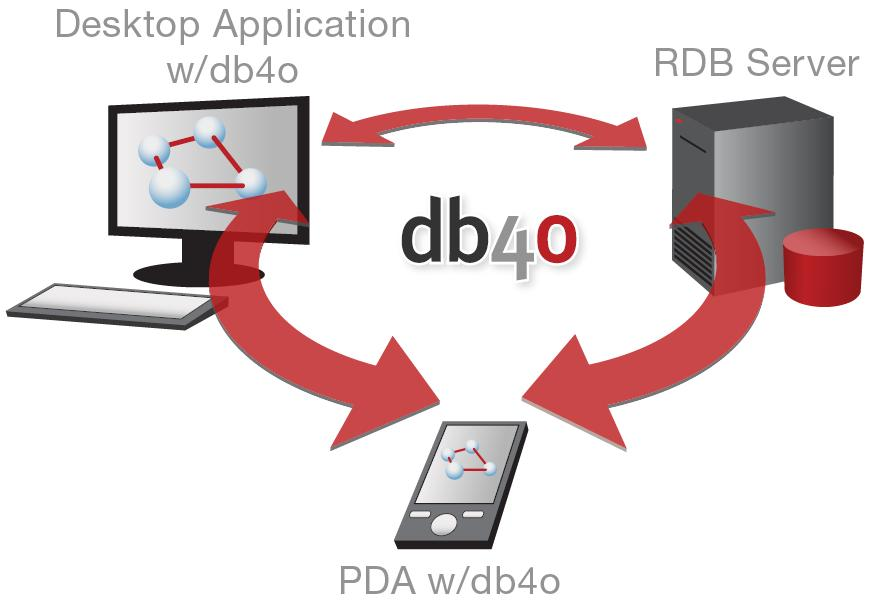
\includegraphics[width=\maxwidth]{images/drs-drsoverview.jpg}
\end{center}
The dRS source code is in the drs directory of the db4o repository at \href{https://github.com/blakemcbride/db4o}{\nolinkurl{github.com/blakemcbride/db4o}}.


% Converted from reference/DRSFlare (MadCap Flare, Java target)

\chapter{Getting Started}
\label{drs:db4o-replication-system-drs-getting-started}

This topic will give you some initial information about dRS and will help to get your environment ready to work with dRS.

\section*{Source Code}

The dRS source code, its libraries and its Ant build file (build.xml) are in the drs directory of the \href{https://github.com/blakemcbride/db4o}{db4o repository}. dRS is not built by the db4o build (BUILD.md); this manual is its documentation.

\section*{Requirements}

The dRS version corresponds to the db4o version. Ensure that the db4o and the dRS version are the same.

The dRS system depends on the JDK 5 version of db4o and therefore requires Java 5 or newer.

In order to use the \hyperref[drs:db4o-replication-system-drs-replication-with-rdbms]{Hibernate-Replication} (p.~\pageref{drs:db4o-replication-system-drs-replication-with-rdbms}) functionality the Hibernate core version 3.1 is required. The Hibernate dependencies are included in the drs/lib directory of the repository for your convenience. When you require more complex Hibernate Mappings or what to benefit from additional Hibernate features, feel free to download the entire Hibernate-distribution on the \href{http://www.hibernate.org/}{Hibernate project website}.

To run the provided ant-scripts \href{http://ant.apache.org/}{Apache Ant 1.6} or later is required.

\section*{Installation}

The dRS functionality is delivered in a single jar file. If you add dRS-8.1-core.jar to your CLASSPATH, dRS is installed. For using db4o replication to another database (RDBMS) you will also need the Hibernate library, which is included in the drs/lib directory of the repository.

Here is how to add the dRS library to an Eclipse project

\begin{itemize}
\item Create a folder named "lib" under your project directory, if it doesn't exist yet
\item Copy dRS-8.1-core.jar to this folder
\item Right-click on your project in the Package Explorer and choose "refresh"
\item Right-click on your project in the Package Explorer again and choose "properties"
\item Select "Java Build Path" in the tree view on the left
\item Select the "Libraries" tab page.
\item Click "Add Jar"
\item The "lib" folder should appear below your project
\item Choose dRS-8.1-core.jar in this folder
\item Hit "OK" twice
\item You might need to repeat the same for hibernate3.jar
\end{itemize}


% Converted from reference/DRSFlare (MadCap Flare, Java target)

\chapter{db4o Databases Replication}
\label{drs:db4o-replication-system-drs-db4o-databases-replication}

The db4o to db4o replication allows you the keep multiple, independent db4o -databases in sync. A typical scenario is when a mobile device is synchronized periodically with the central server or a desktop application

dRS supports simple unidirectional replication where changes are replicated in one direction. \hyperref[drs:db4o-replication-system-drs-db4o-databases-replication-simple-example]{See "Simple Example"} (p.~\pageref{drs:db4o-replication-system-drs-db4o-databases-replication-simple-example})

In addition dRS support bidirectional replication, where changes are replicated in both directions. \hyperref[drs:db4o-replication-system-drs-db4o-databases-replication-bi-directional-replication]{See "Bidirectional Replication"} (p.~\pageref{drs:db4o-replication-system-drs-db4o-databases-replication-bi-directional-replication})

To avoid replicating the whole database, dRS support also partial replication, where only a subset of all objects are replicated. \hyperref[drs:db4o-replication-system-drs-db4o-databases-replication-selective-replication]{See "Selective Replication"} (p.~\pageref{drs:db4o-replication-system-drs-db4o-databases-replication-selective-replication})

Furthermore dRS can also replicate deletions of objects. \hyperref[drs:db4o-replication-system-drs-db4o-databases-replication-deleted-objects-replication]{See "Replicate Deletions"} (p.~\pageref{drs:db4o-replication-system-drs-db4o-databases-replication-deleted-objects-replication})

\section{Simple Example}
\label{drs:db4o-replication-system-drs-db4o-databases-replication-simple-example}

A db4o-to-db4o replication is easy to use and easy to set up. There are only two steps required to get the replication started.

First ensure that you have added the dRS-jar to your project. \hyperref[drs:db4o-replication-system-drs-getting-started]{See "Getting Started"} (p.~\pageref{drs:db4o-replication-system-drs-getting-started})

The replication process needs two things. An UUID for each object to identify it across multiple databases. Furthermore every object needs a version-number to detect updates. By default db4o doesn't generate a UUID nor keeps timestamps. So you need to configure this explicitly:

\begin{lstlisting}
configuration.file().generateUUIDs(ConfigScope.GLOBALLY);
configuration.file().generateCommitTimestamps(true);
\end{lstlisting}

{\small\itshape Db4oReplicationExamples.java: Configure db4o to generate UUIDs and commit timestamps\par}
\medskip

After this preparation you can store, retrieve and update normally. To start the replication-process open the two databases which take part in the replication. Then create an replication-session by passing the replication partners to the replication factory.

\begin{lstlisting}
ObjectContainer desktopDatabase = openDatabase(DESKTOP_DATABASE_NAME);
ObjectContainer mobileDatabase = openDatabase(MOBILE_DATABASE_NAME);

Db4oEmbeddedReplicationProvider providerA = new Db4oEmbeddedReplicationProvider(desktopDatabase);
Db4oEmbeddedReplicationProvider providerB = new Db4oEmbeddedReplicationProvider(mobileDatabase);

ReplicationSession replicationSession = Replication.begin(providerA, providerB);

// set the replication-direction from the desktop database to the mobile database. 
replicationSession.setDirection(replicationSession.providerA(), replicationSession.providerB());
\end{lstlisting}

{\small\itshape Db4oReplicationExamples.java: Prepare unidirectional replication\par}
\medskip

Now the system is ready for replication. First request all changes from a replication partner. The replication session will return all objects which have been created or updated since the last replication. Then iterate over the returned objects and replicate object by object.

\begin{lstlisting}
ObjectSet changes = replicationSession.providerA().objectsChangedSinceLastReplication();
for (Object changedObject : changes) { 
    replicationSession.replicate(changedObject);
}
replicationSession.commit();
\end{lstlisting}

{\small\itshape Db4oReplicationExamples.java: One direction replication\par}
\medskip

To complete the replication, call commit on the replication session. This commit stores all changes in replication partners and finishes the running transactions. Furthermore it marks the objects as replicated to ensure that future replications only include the new changes. Without the commit call the replication-changes will be discarded!

\section{Bidirectional Replication}
\label{drs:db4o-replication-system-drs-db4o-databases-replication-bi-directional-replication}

It's quite often the case that you need replication in both directions. For example when you have a mobile device which keeps the data in sync with a desktop PC. Changes on the both partners have to be replicated to the other partner.

First, make sure that you've prepared and configured db4o properly. \hyperref[drs:db4o-replication-system-drs-db4o-databases-replication-simple-example]{See "Simple Example"} (p.~\pageref{drs:db4o-replication-system-drs-db4o-databases-replication-simple-example})

Start a replication-session with the two replication partners. Note that no replication direction is set.

\begin{lstlisting}
ObjectContainer desktopDatabase = openDatabase(DESKTOP_DATABASE_NAME);
ObjectContainer mobileDatabase = openDatabase(MOBILE_DATABASE_NAME);

Db4oEmbeddedReplicationProvider providerA = new Db4oEmbeddedReplicationProvider(desktopDatabase);
Db4oEmbeddedReplicationProvider providerB = new Db4oEmbeddedReplicationProvider(mobileDatabase);

ReplicationSession replicationSession = Replication.begin(providerA, providerB);
\end{lstlisting}

{\small\itshape Db4oReplicationExamples.java: Prepare bidirectional replication\par}
\medskip

Then get the changed objects from both replication partners. Each replication partner returns the updated and created object in a object-set. Then iterate over both object-sets and replicate the changes.

\begin{lstlisting}
// First get the changes of the two replication-partners
ObjectSet changesOnDesktop = replicationSession.providerA().objectsChangedSinceLastReplication();
ObjectSet changesOnMobile = replicationSession.providerB().objectsChangedSinceLastReplication();

// then iterate over both change-sets and replicate it
for (Object changedObjectOnDesktop : changesOnDesktop) {
    replicationSession.replicate(changedObjectOnDesktop);
}

for (Object changedObjectOnMobile : changesOnMobile) {
    replicationSession.replicate(changedObjectOnMobile);
}

replicationSession.commit();
\end{lstlisting}

{\small\itshape Db4oReplicationExamples.java: Bidirectional replication\par}
\medskip

\section{Selective Replication}
\label{drs:db4o-replication-system-drs-db4o-databases-replication-selective-replication}

What if the mobile device doesn't have enough memory to store all objects? Or if only a subset of the object need to be in both databases? In this case you can replicate only a subset of all objects.

\subsection*{Filter by Class}

You can ask the dRS to replicate only the objects of a certain class. Instead of getting the change-set with all objects, it will return only the changed objects of that class.

\begin{lstlisting}
ObjectSet changesOnDesktop =
    replicationSession.providerA().objectsChangedSinceLastReplication(Pilot.class);

for (Object changedObjectOnDesktop : changesOnDesktop) {
    replicationSession.replicate(changedObjectOnDesktop);
}

replicationSession.commit();
\end{lstlisting}

{\small\itshape Db4oReplicationExamples.java: Selective replication by class\par}
\medskip

\subsection*{Filter With a Condition}

For more complex cases a simple condition can be a solution. Add a simple condition within the replication loop to select which objects are replicated and which ones not.

\begin{lstlisting}
ObjectSet changesOnDesktop = replicationSession.providerA().objectsChangedSinceLastReplication();

for (Object changedObjectOnDesktop : changesOnDesktop) {
    if (changedObjectOnDesktop instanceof Car) {
        if (((Car) changedObjectOnDesktop).getName().startsWith("M")) {
            replicationSession.replicate(changedObjectOnDesktop);
        }
    }            
}

replicationSession.commit();
\end{lstlisting}

{\small\itshape Db4oReplicationExamples.java: Selective replication with a condition\par}
\medskip

\subsection*{Filter With a Query}

It's also possible to query for the objects and the replicate those objects. However in this case, also unchanged objects are replicated again.

\begin{lstlisting}
ObjectSet<Car> changesOnDesktop = desktopDatabase.query(new Predicate<Car>() {
    public boolean match(Car p) {
        return p.getName().startsWith("M");
    }
});

for (Car changedObjectOnDesktop  : changesOnDesktop) {
    replicationSession.replicate(changedObjectOnDesktop);
}

replicationSession.commit();
\end{lstlisting}

{\small\itshape Db4oReplicationExamples.java: Selective replication with a query\par}
\medskip

\subsection*{Combination}

Of course it possible to use a combination of these three possibilities. For example you can request the changes for a certain class and then filter with a condition.

\section{Replicate Deletions}
\label{drs:db4o-replication-system-drs-db4o-databases-replication-deleted-objects-replication}

In addition to replicate new and changed objects, dRS is also able to replicate deletions of objects. By default deletions are not replicated across the databases. When an object is deleted since last replication in one database and you would like to replicate these changes to another database you can use the following method to do this.

\begin{lstlisting}
Db4oEmbeddedReplicationProvider providerA = new Db4oEmbeddedReplicationProvider(desktopDatabase);
Db4oEmbeddedReplicationProvider providerB = new Db4oEmbeddedReplicationProvider(mobileDatabase);

ReplicationSession replicationSession = Replication.begin(providerA, providerB);
replicationSession.replicateDeletions(Car.class);
replicationSession.commit();
\end{lstlisting}

{\small\itshape Db4oReplicationExamples.java: Replicate deletions\par}
\medskip

dRS traverses every Car object in both providers. For instance, if a deleted object is found in one provider, the object will be deleted as well in the other provider.By default the deletion replication is bidirectional. For unidirectional replication set the direction on the replication-session.

Note, that the deletions of a Parent will not be cascaded to child objects. For example, if a Car object is deleted, the Pilots referenced by that Car won't be deleted.


% Converted from reference/DRSFlare (MadCap Flare, Java target)

\chapter{Replication With RDBMS}
\label{drs:db4o-replication-system-drs-replication-with-rdbms}

The Java version of the db4o replication system allows you to replicate to a relational database using \href{http://www.hibernate.org/}{Hibernate}.

Note that dRS needs event handlers which are added to the Hibernate session. It only works when you persist your data through Hibernate.

First you need to setup Hibernate and db4o to support replication. \hyperref[drs:db4o-replication-system-drs-db4o-rdbms-getting-started]{See "Getting Started"} (p.~\pageref{drs:db4o-replication-system-drs-db4o-rdbms-getting-started})

The simplest use case is to replicate from db4o to Hibernate. \hyperref[drs:db4o-replication-system-drs-db4o-rdbms-db4o-to-rdbms]{See "Replicate From db4o To Hibernate"} (p.~\pageref{drs:db4o-replication-system-drs-db4o-rdbms-db4o-to-rdbms}). However most of the time bidirectional replication is the interesting scenario. \hyperref[drs:db4o-replication-system-drs-db4o-rdbms-bi-directional]{See "Bidirectional Replication"} (p.~\pageref{drs:db4o-replication-system-drs-db4o-rdbms-bi-directional})

The enable replication the system has to store additional meta data. \hyperref[drs:db4o-replication-system-drs-db4o-rdbms-drs-internals]{See "dRS Internals"} (p.~\pageref{drs:db4o-replication-system-drs-db4o-rdbms-drs-internals})

Note that the db4o to Hibernate replication has still major limitations. \hyperref[drs:db4o-replication-system-drs-db4o-rdbms-limitations]{See "Limitations"} (p.~\pageref{drs:db4o-replication-system-drs-db4o-rdbms-limitations})

\section{Getting Started}
\label{drs:db4o-replication-system-drs-db4o-rdbms-getting-started}

First you need to add Hibernate. Read the \href{http://www.hibernate.org/docs}{Hibernate documentation} to configure Hibernate properly. This reference documentation only shows the essentials to get started.

\subsection*{Adding The Dependencies}

In order to replicate against Hibernate you need to add the Hibernate jars. The drs/lib directory of the repository contains a copy of Hibernate. dRS is only tested against that Hibernate version. You need to add following dependencies to your project.

\begin{itemize}
\item db4o-8.1-core.jar or db4o-8.1-all.jar
\item dRS-8.1-core.jar
\item All Hibernate dependencies: hibernate3.jar, antlr-2.7.7.jar, jta.jar, commons-logging.jar, commons-collections.jar, dom4j.jar. All other jars are for optional Hibernate features.
\end{itemize}

\subsection*{Configure Hibernate}

Hibernate needs some configuration. You need to configure the database-driver, the database-connection and the SQL dialect. Read more on the \href{https://hibernate.org/orm/documentation/}{official Hibernate documentation}.

\begin{lstlisting}
<hibernate-configuration>
    <session-factory>
        <!-- Specify the database driver -->
        <property name="hibernate.connection.driver_class">org.hsqldb.jdbcDriver</property>

        <!-- The JDBC connection string -->
        <property name="hibernate.connection.url">jdbc:hsqldb:mem:database.hsql</property>

        <!-- User name an password for the database -->
        <property name="hibernate.connection.username">sa</property>
        <property name="hibernate.connection.password"></property>

        <!-- Specify the SQl-dialect -->
        <property name="hibernate.dialect">org.hibernate.dialect.HSQLDialect</property>

        <property name="hibernate.show_sql">true</property>
        <!-- Update the database schema if out of date -->
        <property name="hibernate.hbm2ddl.auto">update</property>

        <!-- Add the mapping files for your classes -->
        <mapping resource="com/db4odoc/drs/rdms/Car.cfg.xml"/>
        <mapping resource="com/db4odoc/drs/rdms/Pilot.cfg.xml"/>

    </session-factory>
</hibernate-configuration>
\end{lstlisting}

{\small\itshape hibernate.cfg.xml: Example Hibernate Configuration\par}
\medskip

\subsection*{Configure The Object Relation Mapping}

In order to store objects in Hibernate, you need define the mapping between the tables and the objects you store. There's only one requirement for the db4o replication: Each object needs a long field for the id. This id is used by dRS to recognize the object. For example we map the Pilot class to the pilots tables. Read more on the \href{https://hibernate.org/orm/documentation/}{official Hibernate documentation}.

\begin{lstlisting}
<hibernate-mapping default-access="field" default-lazy="false" default-cascade="save-update">
    <class name="com.db4odoc.drs.rdms.Pilot" table="pilots">
        <id column="typed_id" type="long">
            <generator class="native"/>
        </id>

        <property name="name"/>
        <property name="points"/>

    </class>
</hibernate-mapping>
\end{lstlisting}

{\small\itshape Pilot.cfg.xml: Mapping the Pilot class\par}
\medskip

\section{Replicate From db4o To Hibernate}
\label{drs:db4o-replication-system-drs-db4o-rdbms-db4o-to-rdbms}

After \hyperref[drs:db4o-replication-system-drs-db4o-rdbms-getting-started]{setting up} (p.~\pageref{drs:db4o-replication-system-drs-db4o-rdbms-getting-started}) Hibernate you can start replicating objects. First you need to configure Hibernate to support the replication system. Additionally you need to enable UUIDs and version numbers on the db4o side.

\begin{lstlisting}
Configuration hibernateConfig
        = new Configuration().configure("com/db4odoc/drs/rdms/hibernate.cfg.xml");
ReplicationConfigurator.configure(hibernateConfig);
\end{lstlisting}

{\small\itshape Db4oRDBMSReplicationExamples.java: Prepare the Hibernate configuration\par}
\medskip

\begin{lstlisting}
configuration.file().generateUUIDs(ConfigScope.GLOBALLY);
configuration.file().generateCommitTimestamps(true);
\end{lstlisting}

{\small\itshape Db4oRDBMSReplicationExamples.java: Configure db4o to generate UUIDs and commit timestamps\par}
\medskip

\subsection*{Start The Replication}

After configuring Hibernate and db4o, the system is ready for replication. Like the \hyperref[drs:db4o-replication-system-drs-db4o-databases-replication-simple-example]{db4o to db4o} (p.~\pageref{drs:db4o-replication-system-drs-db4o-databases-replication-simple-example}) replication you start by creating a replication-session.

\begin{lstlisting}
ObjectContainer container = openDB();

Db4oEmbeddedReplicationProvider providerA = new Db4oEmbeddedReplicationProvider(container);
HibernateReplicationProvider providerB = new HibernateReplicationProvider(hibernateConfig);

ReplicationSession replicationSession = Replication.begin(providerA, providerB);
replicationSession.setDirection(replicationSession.providerA(),replicationSession.providerB());
\end{lstlisting}

{\small\itshape Db4oRDBMSReplicationExamples.java: Prepare replication\par}
\medskip

After that you can request for the changed objects and replicate object by object to Hibernate:

\begin{lstlisting}
final ObjectSet changesInHibernate =
        replicationSession.providerA().objectsChangedSinceLastReplication();
for (Object changedObject : changesInHibernate) {
    replicationSession.replicate(changedObject);
}

replicationSession.commit();
\end{lstlisting}

{\small\itshape Db4oRDBMSReplicationExamples.java: Replicate from db4o to Hibernate\par}
\medskip

\section{Bidirectional Replication}
\label{drs:db4o-replication-system-drs-db4o-rdbms-bi-directional}

In order to replicate objects from Hibernate to db4o you need to do some additional work. dRS needs to know which objects have changed since the last replication. For this some \hyperref[drs:db4o-replication-system-drs-db4o-rdbms-drs-internals]{meta data} (p.~\pageref{drs:db4o-replication-system-drs-db4o-rdbms-drs-internals}) is maintained.You need to register a dRS event handler on every Hibernate-session you're using. This listener will maintain the meta-data. If an object is stored on a session without this listener, the update is not replicated. That also means dRS replication only works when you persist all object through Hibernate

\begin{lstlisting}
SessionFactory sessionFactory = hibernateConfig.buildSessionFactory();
Session session = sessionFactory.openSession();
ReplicationConfigurator.install(session, hibernateConfig);
\end{lstlisting}

{\small\itshape Db4oRDBMSReplicationExamples.java: Install the listeners to the session\par}
\medskip

After that dRS is ready to replicate in both directions. Again, set up the replication-session. After that you can replicate the changes of the two providers in both directions.

\begin{lstlisting}
Configuration hibernateConfig
        = new Configuration().configure("com/db4odoc/drs/rdms/hibernate.cfg.xml");
ObjectContainer container = openDB();

Db4oEmbeddedReplicationProvider providerA = new Db4oEmbeddedReplicationProvider(container);
HibernateReplicationProvider providerB = new HibernateReplicationProvider(hibernateConfig);

ReplicationSession replicationSession = Replication.begin(providerA, providerB);

final ObjectSet changesInDb4o = replicationSession.providerA()
        .objectsChangedSinceLastReplication();
for (Object changedObject : changesInDb4o) {
    replicationSession.replicate(changedObject);
}
final ObjectSet changesInHibernate = replicationSession.providerB()
        .objectsChangedSinceLastReplication();
for (Object changedObject : changesInHibernate) {
    replicationSession.replicate(changedObject);
}
\end{lstlisting}

{\small\itshape Db4oRDBMSReplicationExamples.java: Bidirectional replication\par}
\medskip

\section{dRS Internals}
\label{drs:db4o-replication-system-drs-db4o-rdbms-drs-internals}

How does dRS work to replicate between Hibernate and db4o? This topic gives some insights.

\subsection*{Meta Data}

In order to know which version the objects have and the state of the replication peers dRS needs additional information. For this the dRS system adds extra tables which contain this meta data. These meta data has to maintained, otherwise dRS doesn't replicate the changes. To enable this meta-data tracking you need to add a listener to every Hibernate session:

\begin{lstlisting}
SessionFactory sessionFactory = hibernateConfig.buildSessionFactory();
Session session = sessionFactory.openSession();
ReplicationConfigurator.install(session, hibernateConfig);
\end{lstlisting}

{\small\itshape Db4oRDBMSReplicationExamples.java: Install the listeners to the session\par}
\medskip

\subsubsection*{The Providers}

The providers are the peers which replicate to each others. Each database has a unique identity so that the different providers can be distinguished. This data is kept in the 'drs\_providers' table.

{\small
\begin{longtable}{|p{\dimexpr(\linewidth-4\arrayrulewidth)*1/3-2\tabcolsep\relax}|p{\dimexpr(\linewidth-4\arrayrulewidth)*1/3-2\tabcolsep\relax}|p{\dimexpr(\linewidth-4\arrayrulewidth)*1/3-2\tabcolsep\relax}|}
\hline
\textbf{Column} & \textbf{Type} & \textbf{Purpose} \\ \hline
id & long & Synthetic, auto-increment primary key. \\ \hline
is\_my\_sig & char(1) & 't' when MySignature, 'f' when PeerSignature. \\ \hline
signature & binary & Holds the unique identifier - byte array. \\ \hline
created & long & Legacy field for older versions. \\ \hline
\end{longtable}}

\paragraph*{The History}

The dRS keeps a history of replication with each pair. This history is used to find out when the last replication took place and which objects have changed since the last replication. This data is kept in the 'drs\_history' table.

{\small
\begin{longtable}{|p{\dimexpr(\linewidth-4\arrayrulewidth)*1/3-2\tabcolsep\relax}|p{\dimexpr(\linewidth-4\arrayrulewidth)*1/3-2\tabcolsep\relax}|p{\dimexpr(\linewidth-4\arrayrulewidth)*1/3-2\tabcolsep\relax}|}
\hline
\textbf{Column} & \textbf{Type} & \textbf{Purpose} \\ \hline
provider\_id & long & Primary key, same as the primary key of a provider. \\ \hline
time & long & The last version of the last replication session. \\ \hline
\end{longtable}}

\subsubsection*{The Object Meta Data}

For each object there's meta data. This meta data contains a UUID, the version and some additional information. This data is kept in the 'drs\_objects' table.

{\small
\begin{longtable}{|p{\dimexpr(\linewidth-4\arrayrulewidth)*1/3-2\tabcolsep\relax}|p{\dimexpr(\linewidth-4\arrayrulewidth)*1/3-2\tabcolsep\relax}|p{\dimexpr(\linewidth-4\arrayrulewidth)*1/3-2\tabcolsep\relax}|}
\hline
\textbf{Column} & \textbf{Type} & \textbf{Purpose} \\ \hline
id & long & Synthetic, auto-increment primary key. \\ \hline
created & long & The UUID long part of this ObjectReference. \\ \hline
provider\_id & long & Specifies the originating replication provider of this object. \\ \hline
class\_name & varchar & The type of the referenced object. \\ \hline
typed\_id & long & The id used by Hibernate, which is only unique within its type. \\ \hline
modified & long & The version of the referenced object \\ \hline
\end{longtable}}

\subsection*{Collections}

db4o treats collections like regular objects which have a identity. Hibernate however maps collections to joins and therefore collections don't have an identity. To bridge this gap, dRS treats collections as special objects and does not assign UUIDs to them. However this also means that dRS cannot detect changed collections. So currently you cannot replicate collection-updates between db4o and Hibernate.

\section{Limitations}
\label{drs:db4o-replication-system-drs-db4o-rdbms-limitations}

\subsection*{Collections Limitation}

Collections are treated differently by Hibernate and db4o. In db4o a collection is a regular object. In Hibernate collections are representation of join-operations. This means that collections in Hibernate don't have a identity. That why dRS currently doesn't not track updates on collections when replicating against Hibernate. You only can replicate a collection initially, but cannot replicate updates.


% Converted from reference/DRSFlare (MadCap Flare, Java target)

\chapter{Replication With VOD}
\label{drs:db4o-replication-system-drs-vod-replication}

The Versant Object Database is the 'big brother' of db4o. It's an object database which can deal with a huge amount of data. Because it is also an object database it is a good partner for db4o. For scenarios where you have mobile devices which are synchronized against a big central datastore combining VOD and db4o makes sense. db4o for the mobile end device and VOD on the central server. The Java version of dRS supports therefore this replication between db4o and VOD.

\textbf{Note: Replication with VOD requires at least VOD version 8.0.1.3 with JVI installed.}

The VOD replication partner has to be prepared to be ready for replication. The replication is based on the JDO-interface. Therefore you need to setup and use JDO for the replication. \hyperref[drs:db4o-replication-system-drs-vod-setup]{See "Setup JDO for VOD"} (p.~\pageref{drs:db4o-replication-system-drs-vod-setup})

Additionally a special event processor has to be installed which is responsible to keep track of changes for upcoming replications. \hyperref[drs:db4o-replication-system-drs-vod-setup-event-processing]{See "Setup Event Processing"} (p.~\pageref{drs:db4o-replication-system-drs-vod-setup-event-processing})

After everything is up and running you can start to replicate between db4o and VOD. \hyperref[drs:db4o-replication-system-drs-vod-vod-replication]{See "VOD Replication"} (p.~\pageref{drs:db4o-replication-system-drs-vod-vod-replication})

\section{Setup JDO for VOD}
\label{drs:db4o-replication-system-drs-vod-setup}

This guide shows how to setup JDO for VOD.

This topic assumes that you've already installed the VOD database. VOD is a separate, commercial product, now sold by Actian; follow its installation guide.

\subsection{Create A Database}
\label{drs:db4o-replication-system-drs-vod-setup:createdb}

The first step is to create the database. If you already have a database you can skip this step. The official documentation on managing the VOD database can be found in the VOD installation-folder.

You can create the database with the 'Administration Console' which is shipped with VOD. Start the 'Administration Console', choose 'File'-\textgreater{}'Create Database...' and follow the wizard to create a new database.

As alternative you can create a new database in the command line with these commands:

\begin{lstlisting}
makedb databaseName@localhost
createdb databaseName@localhost
startdb databaseName@localhost
\end{lstlisting}

\subsection{JDO Setup}
\label{drs:db4o-replication-system-drs-vod-setup:jdosetup}

The replication system uses the JDO API to replicate objects between db4o and VOD. Therefore you need to setup the VOD JDO implementation. Again the official documentation is part of the VOD installation. This is just a very short guide to setting JDO up and doesn't cover all details.

First you need to add the JDO-libraries to you project. The JDO-libraries are in the VOD-directory under the 'lib'-subdirectory. You need to add at least these jars.

\begin{itemize}
\item jdo2-api-2.1.jar
\item vodjdo.jar
\item asm-all-3.1.jar
\item jta-1.1.jar
\end{itemize}

Second you need to provide the JDO configuration. You can keep this information in a property file. For example in a versant.properties-file which is stored along with your code. There are three important configuration settings you need to set, the factory-class, the connection-URL and information which classes are enhanced.

For more properties and settings read the JDO and VOD documentation. The example property-file looks like this:

\begin{lstlisting}
## The implementation of the JDO standard
javax.jdo.PersistenceManagerFactoryClass=com.versant.core.jdo.BootstrapPMF
# The connection-string
javax.jdo.option.ConnectionURL=versant:dRSVodExample
# Files which contain a list of meta information for the persistent
# classes. You can list more with versant.metadata.1= versant.metadata.2= ... versant.metadata.n
versant.metadata.0=com/db4odoc/drs/vod/package.jdo
\end{lstlisting}

{\small\itshape versant.properties: JDO configuration for VOD\par}
\medskip

Additionally you need to have a package description where you declare all persistent classes:

\begin{lstlisting}
<jdo>
    <package name="com.db4odoc.drs.vod">
        <class name="com.db4odoc.drs.vod.Car"/>
        <class name="com.db4odoc.drs.vod.Pilot"/>
    </package>
</jdo>
\end{lstlisting}

{\small\itshape package.jdo: List all persistent classes of this package\par}
\medskip

The last preparation step is to get the enhancer in place. JDO requires that classes implements the PersistenceCapable interface. Implementing this by hand would be extremely painful. That's why you can use an enhancer which does this for you. Create an Ant build script which does that.

\begin{lstlisting}
<project name="tutorial" default="build-and-enhance" basedir=".">

    <property file="machine.properties"/>
    <!--The location of the build-result (the compiled class-files).
     Depends on you're build-system / IDE.
     For plain Eclipse projects it's usually "./bin" -->
    <property name="dir.build.output" value="./bin"/>
    <property name="dir.build.source" value="./src"/>
    <property name="dir.lib" value="./lib"/>

    <property name="dir.jdo.lib" value="${dir.vod.install.location}\lib"/>
    <property name="dir.jdo.sdklib" value="${dir.vod.install.location}\sdk\lib"/>

    <path id="enhancerClassPath">
        <pathelement  path="${dir.build.output}"/>
        <fileset dir="${dir.jdo.lib}" includes="**/*.jar"/>
        <fileset dir="${dir.jdo.sdklib}" includes="**/*.jar"/>
    </path>

    <target name="build-and-enhance" depends="compile, enhance"/>

    <target name="enhance" description="Enhance the JOD classes">
        <taskdef resource="versant.tasks">
            <classpath>
                <path refid="enhancerClassPath"/>
            </classpath>
        </taskdef>

        <jdo-enhance outputdir="${dir.build.output}"
                     classpathref="enhancerClassPath" >
            <persistentaware dir="${dir.build.output}"/>
        </jdo-enhance>
    </target>

    <target name="compile">
        <mkdir dir="${dir.build.output}"  />
        <javac srcdir="${dir.build.source}"
            destdir="${dir.build.output}"
            target="6"
            source="6"
            debug="on"
            encoding="UTF-8">
                <classpath>
                    <pathelement path="${dir.jdo.lib}/jdo2-api-2.1.jar"/>
                    <pathelement path="${dir.jdo.lib}/vodjdo.jar"/>
                    <pathelement path="${dir.jdo.lib}/asm-all-3.1.jar"/>
                    <pathelement path="${dir.lib}/*"/>
                </classpath>
            </javac>
        <copy todir="${dir.build.output}">
            <fileset dir="${dir.build.source}" casesensitive="yes">
              <include name="**/*.*"/>
              <exclude name="**/*.java"/>
            </fileset>
        </copy>
    </target>
</project>
\end{lstlisting}

{\small\itshape build.xml: Enhancer script\par}
\medskip

Along to the Ant-script add a machine.properties-file, which contains the installation specific information. Like the installation-location of VOD.

\begin{lstlisting}
# The installation folder of VOD
dir.vod.install.location=C:/progs/Versant/8
\end{lstlisting}

{\small\itshape machine.properties: The properties for our project\par}
\medskip

\subsection{Using JDO}
\label{drs:db4o-replication-system-drs-vod-setup:usingjdo}

After running the enhancer you can start using JDO. First you need to create a PersistenceManagerFactory-instance. This can be created with the static helper methods from the JDOHelper-class:

\begin{lstlisting}
InputStream propertySource = Thread.currentThread()
        .getContextClassLoader().getResourceAsStream(VERSANT_PROPERTY_FILE);
if (null == propertySource) {
    throw new RuntimeException("Couldn't find resource '" + VERSANT_PROPERTY_FILE + "' in the classpath");
}
try {
    return JDOHelper.getPersistenceManagerFactory(propertySource);
} finally {
    try {
        propertySource.close();
    } catch (IOException ignored) {
    }
}
\end{lstlisting}

{\small\itshape JDOUtilities.java: Opening the persistence factory\par}
\medskip

After that you can create persistence manager with the factory and use it to store, query and update objects with JDO:

\begin{lstlisting}
PersistenceManagerFactory factory = JDOUtilities.createPersistenceFactory();

PersistenceManager persistence = factory.getPersistenceManager();
persistence.currentTransaction().begin();

Pilot john = new Pilot("John",42);
Car car = new Car(john,"Fiat Punto");

persistence.makePersistent(car);

persistence.currentTransaction().commit();
persistence.close();
\end{lstlisting}

{\small\itshape StoreObjectsWithJDO.java: Use the persistence manager to store objects\par}
\medskip

For more information and help on JDO read the official VOD documentation and take a look the \href{https://www.datanucleus.org/products/accessplatform/jdo/}{JOD API}.

\section{Setup Event Processing}
\label{drs:db4o-replication-system-drs-vod-setup-event-processing}

The replication system needs to know which objects have been changed in order to replicate these changes. To do so it uses VOD's event system. You need to setup the event processing and keep it running for this purpose.

\textbf{Note: Replication with VOD requires at least VOD version 8.0.1.3 with JVI installed.}

\subsection*{The Classpath}

For the replication operations some additional libraries are required besides the JDO ones. This includes the db4o related libraries and additional VOD libraries.

From the VOD distribution

\begin{itemize}
\item jdo2-api-2.1.jar
\item vodjdo.jar
\item asm-all-3.1.jar
\item antlr-3.1.1-runtime.jar
\item jta-1.1.jar
\item jvi80.jar
\end{itemize}

From db4o / dRS

\begin{itemize}
\item db4o-8.1-core.jar (or db4o-8.1-all.jar)
\item dRS-8.1-core.jar
\end{itemize}

\begin{itemize}
\item commons-cli-1.2.jar
\end{itemize}

\subsection{Creating the Event Schema}
\label{drs:db4o-replication-system-drs-vod-setup-event-processing:eventschema}

The event processing needs special schema's to work correctly. Therefore you need to setup the event schema. You can do this by running the CreateEventSchema-class which does this for you. Pass the database name as argument to that class. You can execute this from the command line, where the classpath contains the libraries from above.

Windows:

\begin{lstlisting}
java -classpath %CLASSPATH% com.db4o.drs.versant.eventprocessor.CreateEventSchema %DATABASE_NAME%
\end{lstlisting}

Unix/Linux:

\begin{lstlisting}
java -classpath $CLASSPATH com.db4o.drs.versant.eventprocessor.CreateEventSchema $DATABASE_NAME
\end{lstlisting}

\subsection{Running The Event Driver}
\label{drs:db4o-replication-system-drs-vod-setup-event-processing:eventdriver}

The next step is to run the VOD event driver. The event driver is a small service application for processing database events. You need to keep the event driver running all the time when you're using replication. Without a running event driver modifications are not replicated. You need to create a configuration file for the event driver.

Windows config.ved.win:

\begin{lstlisting}
ChannelServicePort    4000
LogFile eventdb.log
LogLevel 2
<EngineLibs>
vedse.dll
</EngineLibs>
\end{lstlisting}

Unix/Linux config.ved.linux:

\begin{lstlisting}
ChannelServicePort    4000
LogFile eventdb.log
LogLevel 2
<EngineLibs>
libvedse.so
</EngineLibs>
\end{lstlisting}

With this configuration you can run the event driver. Execute the veddriver command where the first argument is the database name and the second argument is the configuration-file:

\begin{lstlisting}
veddriver %DATABASE_NAME% %VED_CONFIGFILE%
\end{lstlisting}

When veddriver executable is in the 'bin'-subdirectory of your VOD installation.

\subsection{Running The Event Processor}
\label{drs:db4o-replication-system-drs-vod-setup-event-processing:eventprocessor}

After the event driver is up and running we finally can start to process the events. This event processing is there to maintain additional meta-information for the replication process. Ensure that the event processor it always up and running. If it isn't running changes are not replicated.

The event processor is part of the db4o replication system. It's in the EventProcessorApplication-class. This class needs these parameters:

{\small
\begin{longtable}{|p{\dimexpr(\linewidth-4\arrayrulewidth)*1/3-2\tabcolsep\relax}|p{\dimexpr(\linewidth-4\arrayrulewidth)*1/3-2\tabcolsep\relax}|p{\dimexpr(\linewidth-4\arrayrulewidth)*1/3-2\tabcolsep\relax}|}
\hline
-database &  & The name of the database which is replicated \\ \hline
-server & Optional & The host name of the machine where the VOD event driver is running.This a optional parameter. If it's not specified it assumes that the event driver is running on the localhost. \\ \hline
-servertport &  & The port of the VOD event driver. It's the port specified in the event driver configuration. In this example it's 4000 \\ \hline
-client & Optional & The VOD event driver contacts the event processor on certain events. With this parameter you specify the host-name on which the event processor runs. It this parameter is not set localhost will be used. \\ \hline
-clientport &  & The port which is used for the client. It can be any free port. \\ \hline
-eventProcessorPort &  & The port on which the event processor listens for replication processes. The replication process connects to this port. \\ \hline
-logfile &  & Specifies the log file. \\ \hline
-verbose & Optional & Enable the verbose messages \\ \hline
\end{longtable}}

To start the event processor you can use this command. Use the classpath-variable refers to the classpath listed above.

Windows:

\begin{lstlisting}
java -cp %CLASSPATH% com.db4o.drs.versant.eventprocessor.EventProcessorApplication -clientport 4100 -database %DATABASE_NAME% -eventProcessorPort 4088 -logfile %LOG_FILE% -serverport 4000
\end{lstlisting}

Linux:

\begin{lstlisting}
java -cp $CLASSPATH com.db4o.drs.versant.eventprocessor.EventProcessorApplication -clientport 4100 -database $DATABASE_NAME -eventProcessorPort 4088 -logfile $LOG_FILE  -serverport 4000
\end{lstlisting}

\subsection{Example Scripts}
\label{drs:db4o-replication-system-drs-vod-setup-event-processing:examplescripts}

You can use scripts to do this tasks described above. .

You need to adopt the setEnviroment-script to you environment. Specify the path where dRS and db4o jars are. Additionally it expects that the JAVA\_HOME and the VERSANT\_ROOT environment variables are set. The JAVA\_HOME should point to your java-installation. The VERSANT\_ROOT should point to the VOD installation directory.

Windows:

\begin{lstlisting}
REM Specify the directory where the DRS and db4o jars are
REM This directory should contain the db4o and dRS jars.
REM Or more specific it needs the dRS-8.1-core.jar, 
REM db4o-8.1-core.jar or db4o-8.1-core.jar, commons-cli-1.2.jar
SET LIB_DIR=./lib

REM Specify the VOD database name
SET DATABASE_NAME=dRSVodExample

REM Set the directory where VOD is installed. For example "C:\Program Files\Versant\8"
SET VERSANT_ROOT=%VERSANT_ROOT%

REM This should work if the JAVA_HOME variable is set. 
REM Otherwise change the command to point to the java executatble or set the JAVA_HOME variable
SET JAVA=java
JAVA_HOME=$JAVA_HOME
\end{lstlisting}

{\small\itshape setEnvironment.bat: The imporatent configuration items\par}
\medskip

Linux:

\begin{lstlisting}
# Specify the directory where the DRS and db4o jars are
# This directory should contain the db4o and dRS jars.
# Or more specific it needs the dRS-8.1-core.jar, 
# db4o-8.1-core.jar or db4o-8.1-core.jar, commons-cli-1.2.jar
LIB_DIR=./lib

# Specify the VOD database name
DATABASE_NAME=dRSVodExample

# Set the directory where VOD is installed. For example "C:\Program Files\Versant\8"
VERSANT_ROOT=$VERSANT_ROOT

# This should work if the JAVA_HOME variable is set. 
# Otherwise change the command to point to the java executatble or set the JAVA_HOME variable
JAVA=java.exe
JAVA_HOME=$JAVA_HOME
\end{lstlisting}

{\small\itshape setEnvironment.sh: The imporatent configuration items\par}
\medskip

After that you can use the provided scripts to do the steps above.

\begin{itemize}
\item createDatabase: This scripts creates a database with the name configured in DATABASE\_NAME
\item createEventSchema: This script creates the schema for the event processing
\item startEventDriver: This script starts the event driver
\item startEventProcessor: This script starts the event processor
\end{itemize}

\subsection*{Start the Event Driver and Event Processor With Your Database}

In a production environment the event driver and event processor have to run all the time. Therefore it makes sense to start up these two processes together with your database.

You can do this by adding startup entries to your database configuration.

First copy the scripts for starting the event processor to your VOD database directory. Edit the script so that it works from the new location. In the example scripts you probably have to change the directory where the libraries reside.

Second add two new configuration entries to the profile.be file:

\begin{lstlisting}
event_daemon veddriver  the/path/to/config.ved.win
startup_script startEventProcessor.bat
\end{lstlisting}

Then restart the database. These configuration entries should ensure that the event driver and processor are started together with the VOD database.

\section{VOD Replication}
\label{drs:db4o-replication-system-drs-vod-vod-replication}

After setting up \hyperref[drs:db4o-replication-system-drs-vod-setup]{JDO} (p.~\pageref{drs:db4o-replication-system-drs-vod-setup}) and the \hyperref[drs:db4o-replication-system-drs-vod-setup-event-processing]{event processing} (p.~\pageref{drs:db4o-replication-system-drs-vod-setup-event-processing}) we're ready to start the replication.

\textbf{Note: Replication with VOD requires at least VOD version 8.0.1.3 with JVI installed.}

\subsection*{Classpath}

For the VOD replication following libraries need to be in the class-path:

From the VOD distribution

\begin{itemize}
\item jdo2-api-2.1.jar
\item vodjdo.jar
\item asm-all-3.1.jar
\item antlr-3.1.1-runtime.jar
\item jta-1.1.jar
\item jvi80.jar
\end{itemize}

From db4o / dRS

\begin{itemize}
\item db4o-8.1-core.jar (or db4o-8.1-all.jar)
\item dRS-8.1-core.jar
\end{itemize}

\subsection{Prepare db4o}
\label{drs:db4o-replication-system-drs-vod-vod-replication:prepare}

The first thing you need to do is preparing db4o for replication. Enable the UUID and version-number support for your database. UUID's are used to recognize objects across the database boundary. The version number is used the track changes.

Because classes are enhanced for JDO they have additional fields. To avoid that these artificial fields are stored in the db4o database you need to use the JDOReflector. This reflector recognized JDO -aware objects and treats them differently.

\begin{lstlisting}
EmbeddedConfiguration config = Db4oEmbedded.newConfiguration();
config.file().generateUUIDs(ConfigScope.GLOBALLY);
config.file().generateCommitTimestamps(true);
config.common().reflectWith(
        new JdoReflector(Thread.currentThread().getContextClassLoader()));
\end{lstlisting}

{\small\itshape SimpleReplication.java: Enable UUIDs and commit timestamps use the JDO reflector\par}
\medskip

\subsection{Replication From db4o To VOD}
\label{drs:db4o-replication-system-drs-vod-vod-replication:db4otovod}

After this preparation you can store, retrieve and update normally. To start the replication-process you need to create the two replication partners. Open a replication partner for db4o like this:

\begin{lstlisting}
ReplicationProvider mobileDatabase
        = new Db4oEmbeddedReplicationProvider(container);
\end{lstlisting}

{\small\itshape SimpleReplication.java: Open the db4o replication provider\par}
\medskip

Then open a replication provider for VOD. First create a new VodDatabase instance by passing the JDO PersistenceManagerFactory or the \hyperref[drs:db4o-replication-system-drs-vod-setup]{configuration properties} (p.~\pageref{drs:db4o-replication-system-drs-vod-setup}) to the constructor.

Second configure the host and port of the event processor with the configureEventProcessor method. Use the port which you've configured when setting up the \hyperref[drs:db4o-replication-system-drs-vod-setup-event-processing]{event processor} (p.~\pageref{drs:db4o-replication-system-drs-vod-setup-event-processing}). It's the port you've configured with the '-eventProcessorPort'-configuration.

Then create the VOD replication provider. For the VOD replication provider you should additionally add all classes which you want to replicate. Why is this necessary? In VOD you usually have a huge database and you only want to replicate parts of it to db4o. Therefore you can specify which classes are replicated. In case you don't specify anything only the types which have been already replicate once are replicated.

\begin{lstlisting}
VodDatabase vodDatabase = new VodDatabase(factory);
vodDatabase.configureEventProcessor("localhost",4088);
VodReplicationProvider centralDatabase
        = new VodReplicationProvider(vodDatabase);
centralDatabase.listenForReplicationEvents(Car.class, Pilot.class);
\end{lstlisting}

{\small\itshape SimpleReplication.java: Open the VOD replication provider\par}
\medskip

After that you can start the replication. Request the changes from the db4o replication provider. Then iterate over the changed objects and replicate them. Commit to complete the replication process.

\begin{lstlisting}
ReplicationSession replicationSession =
        Replication.begin(mobileDatabase, centralDatabase);

ObjectSet changesOnMobileDB = mobileDatabase.objectsChangedSinceLastReplication();
for (Object changedObject : changesOnMobileDB) {
    replicationSession.replicate(changedObject);
}
replicationSession.commit();
\end{lstlisting}

{\small\itshape SimpleReplication.java: Start replication\par}
\medskip

After this we've replicated the objects from db4o to VOD.

\subsection{Replicate From VOD To db4o}
\label{drs:db4o-replication-system-drs-vod-vod-replication:vodtodb4o}

To replicate from VOD to db4o ensure that you have configured the VOD replication provider properly. You need to add the types which you're going to replicate.

\begin{lstlisting}
VodDatabase vodDatabase = new VodDatabase(factory);
vodDatabase.configureEventProcessor("localhost",4088);
VodReplicationProvider centralDatabase
        = new VodReplicationProvider(vodDatabase);
centralDatabase.listenForReplicationEvents(Car.class, Pilot.class);
\end{lstlisting}

{\small\itshape SimpleReplication.java: Open the VOD replication provider\par}
\medskip

To replicate from VOD to db4o you just need to change the replication direction. Take the changes from the VOD database and replicate them to db4o.

\begin{lstlisting}
ReplicationSession replicationSession =
        Replication.begin(mobileDatabase, centralDatabase);

ObjectSet changesOnVOD = centralDatabase.objectsChangedSinceLastReplication();
for (Object changedObject : changesOnVOD) {
    replicationSession.replicate(changedObject);
}
replicationSession.commit();
\end{lstlisting}

{\small\itshape SimpleReplication.java: From VOD to db4o\par}
\medskip

\subsection{Bidirectional Replication}
\label{drs:db4o-replication-system-drs-vod-vod-replication:bidirectional}

To replicate bidirectional you need to get the changes from both databases and then replicate those changes.

\begin{lstlisting}
ReplicationSession replicationSession =
        Replication.begin(mobileDatabase, centralDatabase);

ObjectSet changesOnDB4O = mobileDatabase.objectsChangedSinceLastReplication();
for (Object changedObject : changesOnDB4O) {
    replicationSession.replicate(changedObject);
}

ObjectSet changesOnVOD = centralDatabase.objectsChangedSinceLastReplication();
for (Object changedObject : changesOnVOD) {
    replicationSession.replicate(changedObject);
}
replicationSession.commit();
\end{lstlisting}

{\small\itshape SimpleReplication.java: Bidirectional replication\par}
\medskip

\section{Replicating to a Mobile Device}
\label{drs:db4o-replication-system-drs-vod-replicating-to-mobile-device}

To replicate against VOD you need all the dependencies for VOD which also includes some native libraries. How can you avoid these extra dependencies?

\subsection{The Workaround}
\label{drs:db4o-replication-system-drs-vod-replicating-to-mobile-device:workaround}

Currently there is one work-around. You can start up a db4o server, which acts an intermediate replication server. The clients replicate against that db4o server and the server then replicates to the VOD server. These are the steps which you need to do:

\begin{enumerate}
\item Setup a db4o server.
\item Setup a periodic replication between the db4o server and VOD.
\item Create the clients, which replicate against the db4o server.
\end{enumerate}

\begin{center}
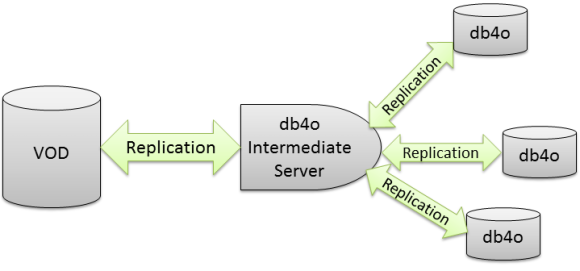
\includegraphics[width=\maxwidth]{images/drs-db4o-replication-system-drs-vod-mobile-replication.png}
\end{center}
\subsection{Setup the Intermediate db4o Server}
\label{drs:db4o-replication-system-drs-vod-replicating-to-mobile-device:intermediate}

The intermediate db4o server will act as replication server. It needs following dependencies:

From the VOD distribution

\begin{itemize}
\item jdo2-api-2.1.jar
\item vodjdo.jar
\item asm-all-3.1.jar
\item antlr-3.1.1-runtime.jar
\item jta-1.1.jar
\item jvi80.jar
\end{itemize}

From db4o / dRS

\begin{itemize}
\item db4o-8.1-core.jar (or db4o-8.1-all.jar)
\item dRS-8.1-core.jar
\end{itemize}

\begin{itemize}
\item db4o-8.1-cs.jar (not needed when you use the db4o-8.1-all.jar)
\end{itemize}

After that you can start a db4o server. Note that it is a pure in memory server, since it does not act a persistent store. For more details take a look at the db4o reference documentation.

\begin{lstlisting}
ServerConfiguration config = Db4oClientServer.newServerConfiguration();
config.file().generateUUIDs(ConfigScope.GLOBALLY);
config.file().generateCommitTimestamps(true);
config.file().storage(new PagingMemoryStorage());
config.common().reflectWith(new JdoReflector(Thread.currentThread().getContextClassLoader()));
ObjectServer server = Db4oClientServer.openServer(config, "!In:Memory!", 8080);
server.grantAccess("sa", "sa");
\end{lstlisting}

{\small\itshape IntermediateDb4oServer.java: Setup server\par}
\medskip

\subsection{Setup Periodic Replication}
\label{drs:db4o-replication-system-drs-vod-replicating-to-mobile-device:periodic}

The next step is to setup periodic replication between the VOD server and the db4o server. Take a look at how to replicate \hyperref[drs:db4o-replication-system-drs-vod-vod-replication]{against VOD here} (p.~\pageref{drs:db4o-replication-system-drs-vod-vod-replication}). The only difference is that it is executed periodically against the intermediate db4o server.

\begin{lstlisting}
final Timer timer = new Timer(true);
timer.schedule(new TimerTask() {
            @Override
            public void run() {
                runReplication();
            }
        },0, TEN_SECONDS_IN_MILLISEC);
\end{lstlisting}

{\small\itshape IntermediateDb4oServer.java: Schedule every 10 seconds\par}
\medskip

The replication against VOD is the same \hyperref[drs:db4o-replication-system-drs-vod-vod-replication]{like here} (p.~\pageref{drs:db4o-replication-system-drs-vod-vod-replication}), but with a db4o client.

\begin{lstlisting}
private void runReplication() {
    ClientConfiguration config = Db4oClientServer.newClientConfiguration();
    config.common().reflectWith(new JdoReflector(Thread.currentThread().getContextClassLoader()));
    ObjectContainer intermediate = Db4oClientServer.openClient(config,"localhost",8080,"sa","sa");
        ReplicationProvider mobileDatabase
            = new Db4oClientServerReplicationProvider(intermediate);
    // The rest is just the regular replication stuff
\end{lstlisting}

{\small\itshape IntermediateDb4oServer.java: Replicate with the db4o server\par}
\medskip

\subsection{The Client}
\label{drs:db4o-replication-system-drs-vod-replicating-to-mobile-device:client}

Now the client doesn't need any VOD dependencies, since we replicate via a db4o server. It needs these dependencies:

\begin{itemize}
\item db4o-8.1-core.jar (or db4o-8.1-all.jar)
\item dRS-8.1-core.jar
\item db4o-8.1-cs.jar (not needed when you use the db4o-8.1-all.jar)
\end{itemize}

Additionally the client needs the classes of the stored objects, but the not enhanced version of the classes. So you have to make sure that you've the original classes on the client and the enhanced classes on the server.

After that the replication is very easy. You just connect to the db4o server and replicate the objects. \hyperref[drs:db4o-replication-system-drs-db4o-databases-replication-bi-directional-replication]{See "Bidirectional Replication"} (p.~\pageref{drs:db4o-replication-system-drs-db4o-databases-replication-bi-directional-replication})

\begin{lstlisting}
EmbeddedConfiguration config = Db4oEmbedded.newConfiguration();
config.file().generateUUIDs(ConfigScope.GLOBALLY);
config.file().generateCommitTimestamps(true);
ObjectContainer theMobileDatabase = Db4oEmbedded.openFile(config, "mobileDatabase.db4o");
ObjectContainer db4oServer = Db4oClientServer.openClient("localhost", 8080, "sa", "sa");
try {
    ReplicationProvider localProvider = new Db4oEmbeddedReplicationProvider(theMobileDatabase);
    ReplicationProvider remoteProvider = new Db4oClientServerReplicationProvider(db4oServer);

    final ReplicationSession replicationSession = Replication.begin(localProvider, remoteProvider);

    replicateAll(replicationSession,localProvider.objectsChangedSinceLastReplication());
    replicateAll(replicationSession,remoteProvider.objectsChangedSinceLastReplication());

    replicationSession.commit();

} catch (Exception e){
    throw new RuntimeException(e);
} finally{
    db4oServer.close();
    theMobileDatabase.close();
}
\end{lstlisting}

{\small\itshape ClientReplicator.java: Replicate against the db4o intermediate server\par}
\medskip


% Converted from reference/DRSFlare (MadCap Flare, Java target)

\chapter{Advanced Replication Strategies}
\label{drs:db4o-replication-system-drs-advanced-replication-strategies}

This topic deals with more complex replication scenarios:

dRS supports events, which you can use to integrate additional logic into the replication. \hyperref[drs:db4o-replication-system-drs-advanced-replication-strategies-events]{See "Events"} (p.~\pageref{drs:db4o-replication-system-drs-advanced-replication-strategies-events})

Sometimes changes on different databases result in a conflict. Then you need to take care it. \hyperref[drs:db4o-replication-system-drs-advanced-replication-strategies-dealing-with-conflicts]{See "Dealing with Conflicts"} (p.~\pageref{drs:db4o-replication-system-drs-advanced-replication-strategies-dealing-with-conflicts})

Maybe you have an existing database which you want to replicate. \hyperref[drs:db4o-replication-system-drs-advanced-replication-strategies-prepare-old-databases-for-replication]{See "Prepare Old Databases for Replication"} (p.~\pageref{drs:db4o-replication-system-drs-advanced-replication-strategies-prepare-old-databases-for-replication})

\section{Events}
\label{drs:db4o-replication-system-drs-advanced-replication-strategies-events}

Often you need more information about the replication process or even need to intervene it. dRS allows the registration of a event listener in order to perform such tasks.

When you create the replication session you can pass such a listener instance. The listener will be called for each object which is replicated.

\begin{lstlisting}
ReplicationSession replicationSession = Replication.begin(providerA, providerB,
        new ReplicationEventListener() {
            public void onReplicate(ReplicationEvent replicationEvent) {
                ObjectState stateInDesktop = replicationEvent.stateInProviderA();
                if (stateInDesktop.isNew()) {
                    System.out.println("Object '"
                            + stateInDesktop.getObject()
                            + "' is new on desktop database");
                }
                if (stateInDesktop.wasModified()) {
                    System.out.println("Object '"
                            + stateInDesktop.getObject()
                            + "' was modified on desktop database");
                }
            }
        });
\end{lstlisting}

{\small\itshape AdvancedReplicationExamples.java: Register a listener for information about the replication process\par}
\medskip

\section{Dealing with Conflicts}
\label{drs:db4o-replication-system-drs-advanced-replication-strategies-dealing-with-conflicts}

When replicated objects are changed independent and the replicated again, conflict are inevitable. The default behavior of dRS is to throw a ReplicationConflictException in such a situation. This prevents corruption, but doesn't help to resolve the conflict. Fortunately dRS allows you to handle such a conflict situation properly.

To deal with conflicts you use a event listener. \hyperref[drs:db4o-replication-system-drs-advanced-replication-strategies-events]{See "Events"} (p.~\pageref{drs:db4o-replication-system-drs-advanced-replication-strategies-events}) . The event has also information about conflicts. When a change conflicts with another change, the conflict flag is set on the replication event. Then you can decide which state is actually replicated. For example: When a conflict occurs you could always take the state of one replication partner.

\begin{lstlisting}
ReplicationSession replicationSession = Replication.begin(providerA, providerB,
        new ReplicationEventListener() {
            public void onReplicate(ReplicationEvent replicationEvent) {
                if (replicationEvent.isConflict()) {
                    ObjectState stateOfTheDesktop = replicationEvent.stateInProviderA();
                    replicationEvent.overrideWith(stateOfTheDesktop);
                }
            }
        });
\end{lstlisting}

{\small\itshape AdvancedReplicationExamples.java: Deal with conflicts\par}
\medskip

Of course there are more advanced strategies possible. For example can compare the timestamp's of the conflicting changes and take the newer change. Note that the clocks of disconnected devices are not perfectly synchronized.

\begin{lstlisting}
ReplicationSession replicationSession = Replication.begin(providerA, providerB,
        new ReplicationEventListener() {
            public void onReplicate(ReplicationEvent replicationEvent) {
                if (replicationEvent.isConflict()) {
                    ObjectState stateDesktop = replicationEvent.stateInProviderA();
                    ObjectState stateMobile = replicationEvent.stateInProviderB();

                    if (stateDesktop.modificationDate() >= stateMobile.modificationDate()) {
                        replicationEvent.overrideWith(stateDesktop);
                    } else {
                        replicationEvent.overrideWith(stateMobile);
                    }
                }
            }
        });
\end{lstlisting}

{\small\itshape AdvancedReplicationExamples.java: Take latest change\par}
\medskip

\section{Prepare Old Databases for Replication}
\label{drs:db4o-replication-system-drs-advanced-replication-strategies-prepare-old-databases-for-replication}

Sometimes replication is a new requirement for a existing application. Therefore existing databases have to be replicated. However the required UUIDs and timestamps haven't been enabled so far. How do you migrate the older databases to enable replication?

The first step is to enable the UUIDs and timestamps.

\begin{lstlisting}
configuration.file().generateUUIDs(ConfigScope.GLOBALLY);
configuration.file().generateCommitTimestamps(true);
\end{lstlisting}

{\small\itshape Db4oReplicationExamples.java: Configure db4o to generate UUIDs and commit timestamps\par}
\medskip

The next issue is that the all objects stored don't have a UUID nor a version numbers. The easiest way to have such a number is to load and update each object in the database. Because when you update a object the new configuration takes effect.

\begin{lstlisting}
ObjectSet<Object> allObjects = desktopDatabase.query(Object.class);
for (Object objectToUpdate : allObjects) {
    desktopDatabase.store(objectToUpdate);
}
desktopDatabase.commit();
\end{lstlisting}

{\small\itshape AdvancedReplicationExamples.java: Updating all objects ensures that it has a UUID and timestamp\par}
\medskip

Updating all object is maybe not an option. It's also possible to do this during the first replication. First query the objects which are target of the replication. Then do the replication. When a object doesn't have a UUID yet, update the object to ensure it has an UUID. Make also sure that the update-depth is high enough so that child objects also have an UUID.

\begin{lstlisting}
Db4oEmbeddedReplicationProvider providerA = new Db4oClientServerReplicationProvider(desktopDatabase);
Db4oEmbeddedReplicationProvider providerB = new Db4oEmbeddedReplicationProvider(mobileDatabase);

ReplicationSession replicationSession = Replication.begin(providerA, providerB);
ObjectSet initialReplication = desktopDatabase.query(Car.class);

for (Object changedObjectOnDesktop : initialReplication) {
    ObjectInfo infoAboutObject = desktopDatabase.ext().getObjectInfo(changedObjectOnDesktop);
    if (null == infoAboutObject.getUUID()) {
        desktopDatabase.ext().store(changedObjectOnDesktop, 2);
    }
    replicationSession.replicate(changedObjectOnDesktop);
}
replicationSession.commit();
\end{lstlisting}

{\small\itshape AdvancedReplicationExamples.java: Migrate on the fly\par}
\medskip


% Converted from reference/DRSFlare (MadCap Flare, Java target)

\chapter{Deployment Instructions}
\label{drs:db4o-replication-system-drs-deployment-instructions}

The dRS version corresponds to the db4o version. Ensure that the db4o and the dRS version are the same.

\section*{db4o to db4o Replication Only}

For a simple db4o to db4o replication scenario you will only need the add the \textbf{dRS-8.1-core.jar.} to the classpath.

\section*{RDBMS Replication}

The RDBMS Replication needs dRS, Hibernate and its dependencies. You need to add the following jars to the classpath:

\begin{itemize}
\item \textbf{dRS-8.1}-core.jar.\textbf{}
\item hibernate3.jar
\item antlr-2.7.6.jar
\item asm.jar
\item asm-attrs.jar
\item cglib-2.1.3.jar
\item commons-collections-2.1.1.jar
\item commons-logging-1.0.4.jar
\item dom4j-1.6.1.jar
\item ehcache-1.2.jar
\item jta.jar
\item log4j-1.2.13.jar
\item xerces-2.6.2.jar
\end{itemize}

Please, refer to the \href{http://www.hibernate.org/}{Hibernate} documentation for an explanation of these dependencies.

If you are going to use dRS with HSQLDB you will need hsqldb-1.8.0.7.jar in addition to Hibernate.


% Converted from reference/DRSFlare (MadCap Flare, Java target)

\chapter{License}
\label{drs:db4o-replication-system-drs-license}

\section*{dRS}

The db4o Replication System (dRS) is available under the General Public License (GPL). Under the GPL dRS is free to be used:

\begin{itemize}
\item for development,
\item in-house as long as no deployment to third parties takes place,
\item together with works that are placed under the GPL themselves.
\end{itemize}

A copy of the GPL is in the file drs/drs.license.html of the \href{https://github.com/blakemcbride/db4o}{db4o repository}.

\section*{Bundled 3rd Party Licenses}

dRS uses several 3rd party libraries, located in the drs/lib directory of the repository together with the respective license files.



\end{document}
